%filename Graphiques-asclepiade
% ltex: language=fr
\documentclass{bio}
\author{Harout CHOULGIAN, Akira LAFOREST et Nicolas LANDUCCI}
\title{Analyse de base de données\\Graphiques préliminaires à titre indicatif}
\teacher{Louis-Philippe Précourt}
\course{BIO-N02}
\group{2}
\department{Biologie}
\date{4 novembre 2025}

\addbibresource{monarques.bib}

\newcommand{\resize}[1]{\resizebox{\textwidth}{!}{#1}}

\begin{document}
\maketitle
%\tocpage


%\section{Introduction}
    CSR: Complètement spatialement aléatoire \textit{Completely spatially random}\nocite{gbif.orgGBIFOccurrenceDownload2025}
    \begin{figure}[H]
        \centering
        \caption{Occurrences de diverses espèces végétales et de lépidoptères à Montréal depuis 2020}
        \resize{%
            % Created by tikzDevice version 0.12.6 on 2025-10-11 22:32:44
% !TEX encoding = UTF-8 Unicode
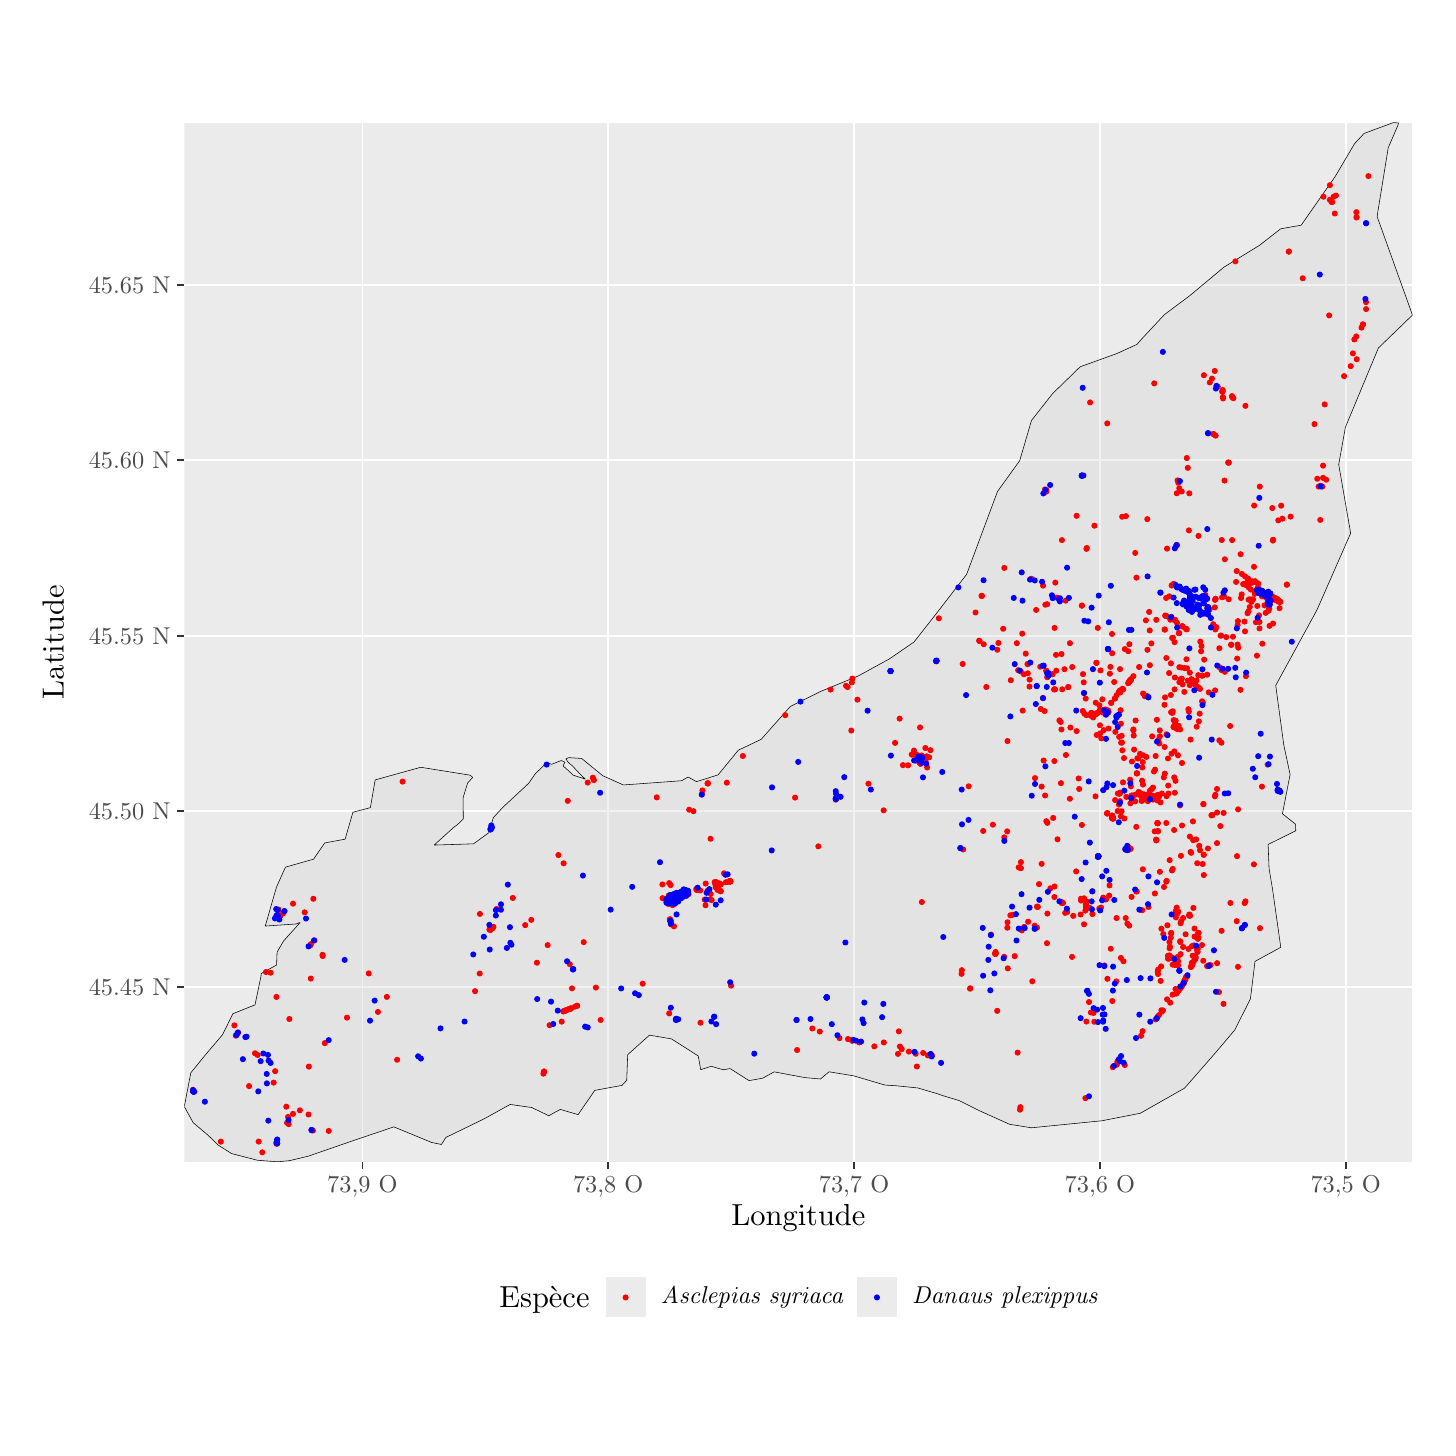
\begin{tikzpicture}[x=1pt,y=1pt]
\definecolor{fillColor}{RGB}{255,255,255}
\path[use as bounding box,fill=fillColor,fill opacity=0.00] (0,0) rectangle (505.89,505.89);
\begin{scope}
\path[clip] (  0.00, 28.82) rectangle (505.89,477.07);
\definecolor{drawColor}{RGB}{255,255,255}
\definecolor{fillColor}{RGB}{255,255,255}

\path[draw=drawColor,line width= 0.6pt,line join=round,line cap=round,fill=fillColor] (  0.00, 28.82) rectangle (505.89,477.07);
\end{scope}
\begin{scope}
\path[clip] ( 56.60, 96.08) rectangle (500.39,471.57);
\definecolor{fillColor}{gray}{0.92}

\path[fill=fillColor] ( 56.60, 96.08) rectangle (500.39,471.57);
\definecolor{drawColor}{RGB}{255,255,255}

\path[draw=drawColor,line width= 0.6pt,line join=round,line cap=round] (120.96, 96.08) --
	(120.96, 99.75) --
	(120.96,103.59) --
	(120.96,107.44) --
	(120.96,111.28) --
	(120.96,115.12) --
	(120.96,118.97) --
	(120.96,122.81) --
	(120.96,126.65) --
	(120.96,130.50) --
	(120.96,134.34) --
	(120.96,138.18) --
	(120.96,142.03) --
	(120.96,145.87) --
	(120.96,149.72) --
	(120.96,153.56) --
	(120.96,157.40) --
	(120.96,161.25) --
	(120.96,165.09) --
	(120.96,168.93) --
	(120.96,172.78) --
	(120.96,176.62) --
	(120.96,180.46) --
	(120.96,184.31) --
	(120.96,188.15) --
	(120.96,191.99) --
	(120.96,195.84) --
	(120.96,199.68) --
	(120.96,203.52) --
	(120.96,207.37) --
	(120.96,211.21) --
	(120.96,215.06) --
	(120.96,218.90) --
	(120.96,222.74) --
	(120.96,226.59) --
	(120.96,230.43) --
	(120.96,234.27) --
	(120.96,238.12) --
	(120.96,241.96) --
	(120.96,245.80) --
	(120.96,249.65) --
	(120.96,253.49) --
	(120.96,257.33) --
	(120.96,261.18) --
	(120.96,265.02) --
	(120.96,268.87) --
	(120.96,272.71) --
	(120.96,276.55) --
	(120.96,280.40) --
	(120.96,284.24) --
	(120.96,288.08) --
	(120.96,291.93) --
	(120.96,295.77) --
	(120.96,299.61) --
	(120.96,303.46) --
	(120.96,307.30) --
	(120.96,311.14) --
	(120.96,314.99) --
	(120.96,318.83) --
	(120.96,322.68) --
	(120.96,326.52) --
	(120.96,330.36) --
	(120.96,334.21) --
	(120.96,338.05) --
	(120.96,341.89) --
	(120.96,345.74) --
	(120.96,349.58) --
	(120.96,353.42) --
	(120.96,357.27) --
	(120.96,361.11) --
	(120.96,364.95) --
	(120.96,368.80) --
	(120.96,372.64) --
	(120.96,376.48) --
	(120.96,380.33) --
	(120.96,384.17) --
	(120.96,388.02) --
	(120.96,391.86) --
	(120.96,395.70) --
	(120.96,399.55) --
	(120.96,403.39) --
	(120.96,407.23) --
	(120.96,411.08) --
	(120.96,414.92) --
	(120.96,418.76) --
	(120.96,422.61) --
	(120.96,426.45) --
	(120.96,430.29) --
	(120.96,434.14) --
	(120.96,437.98) --
	(120.96,441.83) --
	(120.96,445.67) --
	(120.96,449.51) --
	(120.96,453.36) --
	(120.96,457.20) --
	(120.96,461.04) --
	(120.96,464.89) --
	(120.96,468.73) --
	(120.96,471.57);

\path[draw=drawColor,line width= 0.6pt,line join=round,line cap=round] (209.79, 96.08) --
	(209.79, 99.75) --
	(209.79,103.59) --
	(209.79,107.44) --
	(209.79,111.28) --
	(209.79,115.12) --
	(209.79,118.97) --
	(209.79,122.81) --
	(209.79,126.65) --
	(209.79,130.50) --
	(209.79,134.34) --
	(209.79,138.18) --
	(209.79,142.03) --
	(209.79,145.87) --
	(209.79,149.72) --
	(209.79,153.56) --
	(209.79,157.40) --
	(209.79,161.25) --
	(209.79,165.09) --
	(209.79,168.93) --
	(209.79,172.78) --
	(209.79,176.62) --
	(209.79,180.46) --
	(209.79,184.31) --
	(209.79,188.15) --
	(209.79,191.99) --
	(209.79,195.84) --
	(209.79,199.68) --
	(209.79,203.52) --
	(209.79,207.37) --
	(209.79,211.21) --
	(209.79,215.06) --
	(209.79,218.90) --
	(209.79,222.74) --
	(209.79,226.59) --
	(209.79,230.43) --
	(209.79,234.27) --
	(209.79,238.12) --
	(209.79,241.96) --
	(209.79,245.80) --
	(209.79,249.65) --
	(209.79,253.49) --
	(209.79,257.33) --
	(209.79,261.18) --
	(209.79,265.02) --
	(209.79,268.87) --
	(209.79,272.71) --
	(209.79,276.55) --
	(209.79,280.40) --
	(209.79,284.24) --
	(209.79,288.08) --
	(209.79,291.93) --
	(209.79,295.77) --
	(209.79,299.61) --
	(209.79,303.46) --
	(209.79,307.30) --
	(209.79,311.14) --
	(209.79,314.99) --
	(209.79,318.83) --
	(209.79,322.68) --
	(209.79,326.52) --
	(209.79,330.36) --
	(209.79,334.21) --
	(209.79,338.05) --
	(209.79,341.89) --
	(209.79,345.74) --
	(209.79,349.58) --
	(209.79,353.42) --
	(209.79,357.27) --
	(209.79,361.11) --
	(209.79,364.95) --
	(209.79,368.80) --
	(209.79,372.64) --
	(209.79,376.48) --
	(209.79,380.33) --
	(209.79,384.17) --
	(209.79,388.02) --
	(209.79,391.86) --
	(209.79,395.70) --
	(209.79,399.55) --
	(209.79,403.39) --
	(209.79,407.23) --
	(209.79,411.08) --
	(209.79,414.92) --
	(209.79,418.76) --
	(209.79,422.61) --
	(209.79,426.45) --
	(209.79,430.29) --
	(209.79,434.14) --
	(209.79,437.98) --
	(209.79,441.83) --
	(209.79,445.67) --
	(209.79,449.51) --
	(209.79,453.36) --
	(209.79,457.20) --
	(209.79,461.04) --
	(209.79,464.89) --
	(209.79,468.73) --
	(209.79,471.57);

\path[draw=drawColor,line width= 0.6pt,line join=round,line cap=round] (298.61, 96.08) --
	(298.61, 99.75) --
	(298.61,103.59) --
	(298.61,107.44) --
	(298.61,111.28) --
	(298.61,115.12) --
	(298.61,118.97) --
	(298.61,122.81) --
	(298.61,126.65) --
	(298.61,130.50) --
	(298.61,134.34) --
	(298.61,138.18) --
	(298.61,142.03) --
	(298.61,145.87) --
	(298.61,149.72) --
	(298.61,153.56) --
	(298.61,157.40) --
	(298.61,161.25) --
	(298.61,165.09) --
	(298.61,168.93) --
	(298.61,172.78) --
	(298.61,176.62) --
	(298.61,180.46) --
	(298.61,184.31) --
	(298.61,188.15) --
	(298.61,191.99) --
	(298.61,195.84) --
	(298.61,199.68) --
	(298.61,203.52) --
	(298.61,207.37) --
	(298.61,211.21) --
	(298.61,215.06) --
	(298.61,218.90) --
	(298.61,222.74) --
	(298.61,226.59) --
	(298.61,230.43) --
	(298.61,234.27) --
	(298.61,238.12) --
	(298.61,241.96) --
	(298.61,245.80) --
	(298.61,249.65) --
	(298.61,253.49) --
	(298.61,257.33) --
	(298.61,261.18) --
	(298.61,265.02) --
	(298.61,268.87) --
	(298.61,272.71) --
	(298.61,276.55) --
	(298.61,280.40) --
	(298.61,284.24) --
	(298.61,288.08) --
	(298.61,291.93) --
	(298.61,295.77) --
	(298.61,299.61) --
	(298.61,303.46) --
	(298.61,307.30) --
	(298.61,311.14) --
	(298.61,314.99) --
	(298.61,318.83) --
	(298.61,322.68) --
	(298.61,326.52) --
	(298.61,330.36) --
	(298.61,334.21) --
	(298.61,338.05) --
	(298.61,341.89) --
	(298.61,345.74) --
	(298.61,349.58) --
	(298.61,353.42) --
	(298.61,357.27) --
	(298.61,361.11) --
	(298.61,364.95) --
	(298.61,368.80) --
	(298.61,372.64) --
	(298.61,376.48) --
	(298.61,380.33) --
	(298.61,384.17) --
	(298.61,388.02) --
	(298.61,391.86) --
	(298.61,395.70) --
	(298.61,399.55) --
	(298.61,403.39) --
	(298.61,407.23) --
	(298.61,411.08) --
	(298.61,414.92) --
	(298.61,418.76) --
	(298.61,422.61) --
	(298.61,426.45) --
	(298.61,430.29) --
	(298.61,434.14) --
	(298.61,437.98) --
	(298.61,441.83) --
	(298.61,445.67) --
	(298.61,449.51) --
	(298.61,453.36) --
	(298.61,457.20) --
	(298.61,461.04) --
	(298.61,464.89) --
	(298.61,468.73) --
	(298.61,471.57);

\path[draw=drawColor,line width= 0.6pt,line join=round,line cap=round] (387.44, 96.08) --
	(387.44, 99.75) --
	(387.44,103.59) --
	(387.44,107.44) --
	(387.44,111.28) --
	(387.44,115.12) --
	(387.44,118.97) --
	(387.44,122.81) --
	(387.44,126.65) --
	(387.44,130.50) --
	(387.44,134.34) --
	(387.44,138.18) --
	(387.44,142.03) --
	(387.44,145.87) --
	(387.44,149.72) --
	(387.44,153.56) --
	(387.44,157.40) --
	(387.44,161.25) --
	(387.44,165.09) --
	(387.44,168.93) --
	(387.44,172.78) --
	(387.44,176.62) --
	(387.44,180.46) --
	(387.44,184.31) --
	(387.44,188.15) --
	(387.44,191.99) --
	(387.44,195.84) --
	(387.44,199.68) --
	(387.44,203.52) --
	(387.44,207.37) --
	(387.44,211.21) --
	(387.44,215.06) --
	(387.44,218.90) --
	(387.44,222.74) --
	(387.44,226.59) --
	(387.44,230.43) --
	(387.44,234.27) --
	(387.44,238.12) --
	(387.44,241.96) --
	(387.44,245.80) --
	(387.44,249.65) --
	(387.44,253.49) --
	(387.44,257.33) --
	(387.44,261.18) --
	(387.44,265.02) --
	(387.44,268.87) --
	(387.44,272.71) --
	(387.44,276.55) --
	(387.44,280.40) --
	(387.44,284.24) --
	(387.44,288.08) --
	(387.44,291.93) --
	(387.44,295.77) --
	(387.44,299.61) --
	(387.44,303.46) --
	(387.44,307.30) --
	(387.44,311.14) --
	(387.44,314.99) --
	(387.44,318.83) --
	(387.44,322.68) --
	(387.44,326.52) --
	(387.44,330.36) --
	(387.44,334.21) --
	(387.44,338.05) --
	(387.44,341.89) --
	(387.44,345.74) --
	(387.44,349.58) --
	(387.44,353.42) --
	(387.44,357.27) --
	(387.44,361.11) --
	(387.44,364.95) --
	(387.44,368.80) --
	(387.44,372.64) --
	(387.44,376.48) --
	(387.44,380.33) --
	(387.44,384.17) --
	(387.44,388.02) --
	(387.44,391.86) --
	(387.44,395.70) --
	(387.44,399.55) --
	(387.44,403.39) --
	(387.44,407.23) --
	(387.44,411.08) --
	(387.44,414.92) --
	(387.44,418.76) --
	(387.44,422.61) --
	(387.44,426.45) --
	(387.44,430.29) --
	(387.44,434.14) --
	(387.44,437.98) --
	(387.44,441.83) --
	(387.44,445.67) --
	(387.44,449.51) --
	(387.44,453.36) --
	(387.44,457.20) --
	(387.44,461.04) --
	(387.44,464.89) --
	(387.44,468.73) --
	(387.44,471.57);

\path[draw=drawColor,line width= 0.6pt,line join=round,line cap=round] (476.26, 96.08) --
	(476.26, 99.75) --
	(476.26,103.59) --
	(476.26,107.44) --
	(476.26,111.28) --
	(476.26,115.12) --
	(476.26,118.97) --
	(476.26,122.81) --
	(476.26,126.65) --
	(476.26,130.50) --
	(476.26,134.34) --
	(476.26,138.18) --
	(476.26,142.03) --
	(476.26,145.87) --
	(476.26,149.72) --
	(476.26,153.56) --
	(476.26,157.40) --
	(476.26,161.25) --
	(476.26,165.09) --
	(476.26,168.93) --
	(476.26,172.78) --
	(476.26,176.62) --
	(476.26,180.46) --
	(476.26,184.31) --
	(476.26,188.15) --
	(476.26,191.99) --
	(476.26,195.84) --
	(476.26,199.68) --
	(476.26,203.52) --
	(476.26,207.37) --
	(476.26,211.21) --
	(476.26,215.06) --
	(476.26,218.90) --
	(476.26,222.74) --
	(476.26,226.59) --
	(476.26,230.43) --
	(476.26,234.27) --
	(476.26,238.12) --
	(476.26,241.96) --
	(476.26,245.80) --
	(476.26,249.65) --
	(476.26,253.49) --
	(476.26,257.33) --
	(476.26,261.18) --
	(476.26,265.02) --
	(476.26,268.87) --
	(476.26,272.71) --
	(476.26,276.55) --
	(476.26,280.40) --
	(476.26,284.24) --
	(476.26,288.08) --
	(476.26,291.93) --
	(476.26,295.77) --
	(476.26,299.61) --
	(476.26,303.46) --
	(476.26,307.30) --
	(476.26,311.14) --
	(476.26,314.99) --
	(476.26,318.83) --
	(476.26,322.68) --
	(476.26,326.52) --
	(476.26,330.36) --
	(476.26,334.21) --
	(476.26,338.05) --
	(476.26,341.89) --
	(476.26,345.74) --
	(476.26,349.58) --
	(476.26,353.42) --
	(476.26,357.27) --
	(476.26,361.11) --
	(476.26,364.95) --
	(476.26,368.80) --
	(476.26,372.64) --
	(476.26,376.48) --
	(476.26,380.33) --
	(476.26,384.17) --
	(476.26,388.02) --
	(476.26,391.86) --
	(476.26,395.70) --
	(476.26,399.55) --
	(476.26,403.39) --
	(476.26,407.23) --
	(476.26,411.08) --
	(476.26,414.92) --
	(476.26,418.76) --
	(476.26,422.61) --
	(476.26,426.45) --
	(476.26,430.29) --
	(476.26,434.14) --
	(476.26,437.98) --
	(476.26,441.83) --
	(476.26,445.67) --
	(476.26,449.51) --
	(476.26,453.36) --
	(476.26,457.20) --
	(476.26,461.04) --
	(476.26,464.89) --
	(476.26,468.73) --
	(476.26,471.57);

\path[draw=drawColor,line width= 0.6pt,line join=round,line cap=round] ( 56.60,159.32) --
	( 59.05,159.32) --
	( 64.44,159.32) --
	( 69.82,159.32) --
	( 75.20,159.32) --
	( 80.59,159.32) --
	( 85.97,159.32) --
	( 91.35,159.32) --
	( 96.74,159.32) --
	(102.12,159.32) --
	(107.50,159.32) --
	(112.89,159.32) --
	(118.27,159.32) --
	(123.65,159.32) --
	(129.04,159.32) --
	(134.42,159.32) --
	(139.80,159.32) --
	(145.19,159.32) --
	(150.57,159.32) --
	(155.95,159.32) --
	(161.34,159.32) --
	(166.72,159.32) --
	(172.10,159.32) --
	(177.49,159.32) --
	(182.87,159.32) --
	(188.25,159.32) --
	(193.64,159.32) --
	(199.02,159.32) --
	(204.40,159.32) --
	(209.79,159.32) --
	(215.17,159.32) --
	(220.55,159.32) --
	(225.94,159.32) --
	(231.32,159.32) --
	(236.70,159.32) --
	(242.09,159.32) --
	(247.47,159.32) --
	(252.85,159.32) --
	(258.24,159.32) --
	(263.62,159.32) --
	(269.00,159.32) --
	(274.39,159.32) --
	(279.77,159.32) --
	(285.15,159.32) --
	(290.54,159.32) --
	(295.92,159.32) --
	(301.31,159.32) --
	(306.69,159.32) --
	(312.07,159.32) --
	(317.46,159.32) --
	(322.84,159.32) --
	(328.22,159.32) --
	(333.61,159.32) --
	(338.99,159.32) --
	(344.37,159.32) --
	(349.76,159.32) --
	(355.14,159.32) --
	(360.52,159.32) --
	(365.91,159.32) --
	(371.29,159.32) --
	(376.67,159.32) --
	(382.06,159.32) --
	(387.44,159.32) --
	(392.82,159.32) --
	(398.21,159.32) --
	(403.59,159.32) --
	(408.97,159.32) --
	(414.36,159.32) --
	(419.74,159.32) --
	(425.12,159.32) --
	(430.51,159.32) --
	(435.89,159.32) --
	(441.27,159.32) --
	(446.66,159.32) --
	(452.04,159.32) --
	(457.42,159.32) --
	(462.81,159.32) --
	(468.19,159.32) --
	(473.57,159.32) --
	(478.96,159.32) --
	(484.34,159.32) --
	(489.72,159.32) --
	(495.11,159.32) --
	(500.39,159.32);

\path[draw=drawColor,line width= 0.6pt,line join=round,line cap=round] ( 56.60,222.74) --
	( 59.05,222.74) --
	( 64.44,222.74) --
	( 69.82,222.74) --
	( 75.20,222.74) --
	( 80.59,222.74) --
	( 85.97,222.74) --
	( 91.35,222.74) --
	( 96.74,222.74) --
	(102.12,222.74) --
	(107.50,222.74) --
	(112.89,222.74) --
	(118.27,222.74) --
	(123.65,222.74) --
	(129.04,222.74) --
	(134.42,222.74) --
	(139.80,222.74) --
	(145.19,222.74) --
	(150.57,222.74) --
	(155.95,222.74) --
	(161.34,222.74) --
	(166.72,222.74) --
	(172.10,222.74) --
	(177.49,222.74) --
	(182.87,222.74) --
	(188.25,222.74) --
	(193.64,222.74) --
	(199.02,222.74) --
	(204.40,222.74) --
	(209.79,222.74) --
	(215.17,222.74) --
	(220.55,222.74) --
	(225.94,222.74) --
	(231.32,222.74) --
	(236.70,222.74) --
	(242.09,222.74) --
	(247.47,222.74) --
	(252.85,222.74) --
	(258.24,222.74) --
	(263.62,222.74) --
	(269.00,222.74) --
	(274.39,222.74) --
	(279.77,222.74) --
	(285.15,222.74) --
	(290.54,222.74) --
	(295.92,222.74) --
	(301.31,222.74) --
	(306.69,222.74) --
	(312.07,222.74) --
	(317.46,222.74) --
	(322.84,222.74) --
	(328.22,222.74) --
	(333.61,222.74) --
	(338.99,222.74) --
	(344.37,222.74) --
	(349.76,222.74) --
	(355.14,222.74) --
	(360.52,222.74) --
	(365.91,222.74) --
	(371.29,222.74) --
	(376.67,222.74) --
	(382.06,222.74) --
	(387.44,222.74) --
	(392.82,222.74) --
	(398.21,222.74) --
	(403.59,222.74) --
	(408.97,222.74) --
	(414.36,222.74) --
	(419.74,222.74) --
	(425.12,222.74) --
	(430.51,222.74) --
	(435.89,222.74) --
	(441.27,222.74) --
	(446.66,222.74) --
	(452.04,222.74) --
	(457.42,222.74) --
	(462.81,222.74) --
	(468.19,222.74) --
	(473.57,222.74) --
	(478.96,222.74) --
	(484.34,222.74) --
	(489.72,222.74) --
	(495.11,222.74) --
	(500.39,222.74);

\path[draw=drawColor,line width= 0.6pt,line join=round,line cap=round] ( 56.60,286.16) --
	( 59.05,286.16) --
	( 64.44,286.16) --
	( 69.82,286.16) --
	( 75.20,286.16) --
	( 80.59,286.16) --
	( 85.97,286.16) --
	( 91.35,286.16) --
	( 96.74,286.16) --
	(102.12,286.16) --
	(107.50,286.16) --
	(112.89,286.16) --
	(118.27,286.16) --
	(123.65,286.16) --
	(129.04,286.16) --
	(134.42,286.16) --
	(139.80,286.16) --
	(145.19,286.16) --
	(150.57,286.16) --
	(155.95,286.16) --
	(161.34,286.16) --
	(166.72,286.16) --
	(172.10,286.16) --
	(177.49,286.16) --
	(182.87,286.16) --
	(188.25,286.16) --
	(193.64,286.16) --
	(199.02,286.16) --
	(204.40,286.16) --
	(209.79,286.16) --
	(215.17,286.16) --
	(220.55,286.16) --
	(225.94,286.16) --
	(231.32,286.16) --
	(236.70,286.16) --
	(242.09,286.16) --
	(247.47,286.16) --
	(252.85,286.16) --
	(258.24,286.16) --
	(263.62,286.16) --
	(269.00,286.16) --
	(274.39,286.16) --
	(279.77,286.16) --
	(285.15,286.16) --
	(290.54,286.16) --
	(295.92,286.16) --
	(301.31,286.16) --
	(306.69,286.16) --
	(312.07,286.16) --
	(317.46,286.16) --
	(322.84,286.16) --
	(328.22,286.16) --
	(333.61,286.16) --
	(338.99,286.16) --
	(344.37,286.16) --
	(349.76,286.16) --
	(355.14,286.16) --
	(360.52,286.16) --
	(365.91,286.16) --
	(371.29,286.16) --
	(376.67,286.16) --
	(382.06,286.16) --
	(387.44,286.16) --
	(392.82,286.16) --
	(398.21,286.16) --
	(403.59,286.16) --
	(408.97,286.16) --
	(414.36,286.16) --
	(419.74,286.16) --
	(425.12,286.16) --
	(430.51,286.16) --
	(435.89,286.16) --
	(441.27,286.16) --
	(446.66,286.16) --
	(452.04,286.16) --
	(457.42,286.16) --
	(462.81,286.16) --
	(468.19,286.16) --
	(473.57,286.16) --
	(478.96,286.16) --
	(484.34,286.16) --
	(489.72,286.16) --
	(495.11,286.16) --
	(500.39,286.16);

\path[draw=drawColor,line width= 0.6pt,line join=round,line cap=round] ( 56.60,349.58) --
	( 59.05,349.58) --
	( 64.44,349.58) --
	( 69.82,349.58) --
	( 75.20,349.58) --
	( 80.59,349.58) --
	( 85.97,349.58) --
	( 91.35,349.58) --
	( 96.74,349.58) --
	(102.12,349.58) --
	(107.50,349.58) --
	(112.89,349.58) --
	(118.27,349.58) --
	(123.65,349.58) --
	(129.04,349.58) --
	(134.42,349.58) --
	(139.80,349.58) --
	(145.19,349.58) --
	(150.57,349.58) --
	(155.95,349.58) --
	(161.34,349.58) --
	(166.72,349.58) --
	(172.10,349.58) --
	(177.49,349.58) --
	(182.87,349.58) --
	(188.25,349.58) --
	(193.64,349.58) --
	(199.02,349.58) --
	(204.40,349.58) --
	(209.79,349.58) --
	(215.17,349.58) --
	(220.55,349.58) --
	(225.94,349.58) --
	(231.32,349.58) --
	(236.70,349.58) --
	(242.09,349.58) --
	(247.47,349.58) --
	(252.85,349.58) --
	(258.24,349.58) --
	(263.62,349.58) --
	(269.00,349.58) --
	(274.39,349.58) --
	(279.77,349.58) --
	(285.15,349.58) --
	(290.54,349.58) --
	(295.92,349.58) --
	(301.31,349.58) --
	(306.69,349.58) --
	(312.07,349.58) --
	(317.46,349.58) --
	(322.84,349.58) --
	(328.22,349.58) --
	(333.61,349.58) --
	(338.99,349.58) --
	(344.37,349.58) --
	(349.76,349.58) --
	(355.14,349.58) --
	(360.52,349.58) --
	(365.91,349.58) --
	(371.29,349.58) --
	(376.67,349.58) --
	(382.06,349.58) --
	(387.44,349.58) --
	(392.82,349.58) --
	(398.21,349.58) --
	(403.59,349.58) --
	(408.97,349.58) --
	(414.36,349.58) --
	(419.74,349.58) --
	(425.12,349.58) --
	(430.51,349.58) --
	(435.89,349.58) --
	(441.27,349.58) --
	(446.66,349.58) --
	(452.04,349.58) --
	(457.42,349.58) --
	(462.81,349.58) --
	(468.19,349.58) --
	(473.57,349.58) --
	(478.96,349.58) --
	(484.34,349.58) --
	(489.72,349.58) --
	(495.11,349.58) --
	(500.39,349.58);

\path[draw=drawColor,line width= 0.6pt,line join=round,line cap=round] ( 56.60,413.00) --
	( 59.05,413.00) --
	( 64.44,413.00) --
	( 69.82,413.00) --
	( 75.20,413.00) --
	( 80.59,413.00) --
	( 85.97,413.00) --
	( 91.35,413.00) --
	( 96.74,413.00) --
	(102.12,413.00) --
	(107.50,413.00) --
	(112.89,413.00) --
	(118.27,413.00) --
	(123.65,413.00) --
	(129.04,413.00) --
	(134.42,413.00) --
	(139.80,413.00) --
	(145.19,413.00) --
	(150.57,413.00) --
	(155.95,413.00) --
	(161.34,413.00) --
	(166.72,413.00) --
	(172.10,413.00) --
	(177.49,413.00) --
	(182.87,413.00) --
	(188.25,413.00) --
	(193.64,413.00) --
	(199.02,413.00) --
	(204.40,413.00) --
	(209.79,413.00) --
	(215.17,413.00) --
	(220.55,413.00) --
	(225.94,413.00) --
	(231.32,413.00) --
	(236.70,413.00) --
	(242.09,413.00) --
	(247.47,413.00) --
	(252.85,413.00) --
	(258.24,413.00) --
	(263.62,413.00) --
	(269.00,413.00) --
	(274.39,413.00) --
	(279.77,413.00) --
	(285.15,413.00) --
	(290.54,413.00) --
	(295.92,413.00) --
	(301.31,413.00) --
	(306.69,413.00) --
	(312.07,413.00) --
	(317.46,413.00) --
	(322.84,413.00) --
	(328.22,413.00) --
	(333.61,413.00) --
	(338.99,413.00) --
	(344.37,413.00) --
	(349.76,413.00) --
	(355.14,413.00) --
	(360.52,413.00) --
	(365.91,413.00) --
	(371.29,413.00) --
	(376.67,413.00) --
	(382.06,413.00) --
	(387.44,413.00) --
	(392.82,413.00) --
	(398.21,413.00) --
	(403.59,413.00) --
	(408.97,413.00) --
	(414.36,413.00) --
	(419.74,413.00) --
	(425.12,413.00) --
	(430.51,413.00) --
	(435.89,413.00) --
	(441.27,413.00) --
	(446.66,413.00) --
	(452.04,413.00) --
	(457.42,413.00) --
	(462.81,413.00) --
	(468.19,413.00) --
	(473.57,413.00) --
	(478.96,413.00) --
	(484.34,413.00) --
	(489.72,413.00) --
	(495.11,413.00) --
	(500.39,413.00);
\definecolor{drawColor}{RGB}{0,0,0}
\definecolor{fillColor}{RGB}{211,211,211}

\path[draw=drawColor,line width= 0.2pt,line join=round,fill=fillColor,fill opacity=0.30,even odd rule]
	(101.38, 98.10) --
	( 98.88, 97.50) --
	( 97.78, 97.24) --
	( 96.63, 96.97) --
	( 95.12, 96.61) --
	( 94.55, 96.47) --
	( 92.38, 96.27) --
	( 90.71, 96.11) --
	( 90.34, 96.08) --
	( 90.23, 96.09) --
	( 89.25, 96.16) --
	( 85.00, 96.48) --
	( 83.83, 96.57) --
	( 83.09, 96.62) --
	( 73.70, 99.04) --
	( 72.52, 99.78) --
	( 68.74,102.18) --
	( 66.74,104.14) --
	( 66.31,104.57) --
	( 65.20,105.65) --
	( 61.20,109.03) --
	( 59.80,110.22) --
	( 58.71,112.21) --
	( 56.60,116.04) --
	( 56.89,117.54) --
	( 57.52,120.83) --
	( 58.36,125.16) --
	( 58.95,128.23) --
	( 64.34,134.86) --
	( 70.39,141.97) --
	( 71.16,143.54) --
	( 71.38,143.97) --
	( 73.02,147.28) --
	( 74.15,149.58) --
	( 76.25,150.42) --
	( 76.36,150.46) --
	( 76.51,150.52) --
	( 82.15,152.78) --
	( 84.27,162.97) --
	( 84.31,163.35) --
	( 84.41,164.12) --
	( 85.63,164.80) --
	( 87.54,165.86) --
	( 89.02,166.68) --
	( 89.94,167.19) --
	( 89.98,168.26) --
	( 90.07,170.47) --
	( 90.12,171.82) --
	( 92.44,175.83) --
	( 94.21,177.80) --
	( 97.53,181.49) --
	( 98.43,182.48) --
	( 97.87,182.39) --
	( 97.47,182.21) --
	( 97.41,182.18) --
	( 97.05,182.01) --
	( 85.85,181.26) --
	( 88.14,189.21) --
	( 88.28,189.71) --
	( 88.81,191.54) --
	( 89.90,195.30) --
	( 92.19,200.42) --
	( 93.15,202.54) --
	(103.31,205.44) --
	(105.03,207.95) --
	(107.33,211.29) --
	(110.40,211.86) --
	(111.65,212.09) --
	(114.71,212.65) --
	(116.31,218.19) --
	(117.52,222.37) --
	(119.19,222.82) --
	(123.83,224.04) --
	(125.57,234.07) --
	(127.70,234.66) --
	(142.05,238.63) --
	(157.73,236.12) --
	(159.88,235.77) --
	(160.82,234.99) --
	(160.63,234.78) --
	(159.26,233.25) --
	(158.99,232.95) --
	(158.61,231.75) --
	(158.13,230.19) --
	(157.35,227.70) --
	(157.38,223.47) --
	(157.39,221.65) --
	(157.41,220.02) --
	(157.06,219.62) --
	(156.84,219.38) --
	(156.74,219.27) --
	(156.41,218.93) --
	(156.33,218.85) --
	(156.24,218.77) --
	(156.07,218.60) --
	(155.77,218.33) --
	(155.67,218.25) --
	(155.35,217.97) --
	(154.97,217.68) --
	(154.79,217.54) --
	(154.66,217.44) --
	(154.59,217.39) --
	(154.38,217.25) --
	(154.28,217.18) --
	(154.19,217.13) --
	(146.88,210.52) --
	(151.70,210.67) --
	(155.52,210.79) --
	(157.65,210.86) --
	(157.85,210.87) --
	(161.12,210.97) --
	(162.59,212.05) --
	(164.83,213.68) --
	(166.70,215.04) --
	(166.89,215.68) --
	(167.08,216.36) --
	(167.83,218.94) --
	(168.26,220.44) --
	(169.98,222.30) --
	(171.67,224.13) --
	(175.70,227.88) --
	(177.16,229.23) --
	(181.04,232.84) --
	(183.41,236.28) --
	(185.14,237.96) --
	(187.52,240.27) --
	(189.31,239.72) --
	(190.83,240.30) --
	(192.76,241.05) --
	(193.37,240.85) --
	(194.10,240.46) --
	(193.72,239.67) --
	(193.51,239.10) --
	(196.40,236.48) --
	(197.15,235.76) --
	(198.42,235.36) --
	(201.46,234.37) --
	(199.29,236.51) --
	(196.77,239.21) --
	(196.22,239.63) --
	(195.39,240.34) --
	(194.84,241.09) --
	(194.84,241.24) --
	(194.68,241.41) --
	(194.44,241.69) --
	(195.54,242.12) --
	(199.87,241.84) --
	(200.19,241.82) --
	(207.80,235.58) --
	(213.22,233.15) --
	(214.78,232.45) --
	(215.24,232.24) --
	(225.32,232.97) --
	(236.30,233.77) --
	(238.07,234.79) --
	(238.63,235.11) --
	(239.03,234.90) --
	(241.67,233.44) --
	(245.07,234.50) --
	(245.42,234.61) --
	(246.12,234.83) --
	(246.41,234.92) --
	(249.48,235.89) --
	(256.80,244.81) --
	(257.69,245.23) --
	(265.04,248.72) --
	(268.95,253.13) --
	(275.62,260.64) --
	(278.13,261.88) --
	(279.21,262.41) --
	(283.87,264.71) --
	(286.67,266.09) --
	(288.42,266.81) --
	(290.58,267.70) --
	(298.80,271.08) --
	(300.12,271.63) --
	(307.21,275.51) --
	(307.60,275.73) --
	(311.39,277.80) --
	(314.67,280.05) --
	(320.27,283.89) --
	(327.84,293.53) --
	(332.67,299.78) --
	(339.29,308.35) --
	(343.51,319.68) --
	(345.35,324.63) --
	(345.41,324.79) --
	(347.98,331.69) --
	(350.45,338.31) --
	(352.21,340.74) --
	(353.53,342.58) --
	(358.46,349.41) --
	(359.01,351.29) --
	(360.30,355.67) --
	(362.35,362.67) --
	(362.74,363.98) --
	(365.06,366.93) --
	(370.32,373.62) --
	(373.67,376.88) --
	(375.61,378.77) --
	(375.84,378.99) --
	(378.68,381.76) --
	(380.30,383.34) --
	(383.96,384.66) --
	(393.57,388.13) --
	(397.82,390.07) --
	(398.23,390.25) --
	(398.51,390.38) --
	(400.86,391.45) --
	(401.47,392.16) --
	(402.21,393.04) --
	(410.79,402.23) --
	(417.34,407.12) --
	(419.80,408.95) --
	(423.12,411.72) --
	(432.24,419.33) --
	(438.97,423.46) --
	(445.13,427.25) --
	(446.80,428.55) --
	(452.76,433.20) --
	(457.02,433.96) --
	(457.71,434.08) --
	(460.18,434.51) --
	(467.02,444.31) --
	(468.32,446.18) --
	(468.93,447.05) --
	(470.30,449.00) --
	(472.40,452.01) --
	(479.48,463.99) --
	(482.13,466.83) --
	(482.91,467.67) --
	(488.07,469.58) --
	(493.46,471.57) --
	(494.55,471.52) --
	(495.35,471.49) --
	(495.16,470.71) --
	(495.14,470.62) --
	(495.04,470.40) --
	(494.95,470.21) --
	(494.78,469.79) --
	(491.62,462.47) --
	(491.45,461.41) --
	(491.38,460.93) --
	(487.95,439.76) --
	(487.70,438.18) --
	(487.62,437.65) --
	(487.72,437.37) --
	(487.82,437.08) --
	(494.45,418.58) --
	(500.06,402.96) --
	(500.12,402.79) --
	(500.17,402.66) --
	(500.23,402.46) --
	(500.29,402.29) --
	(500.39,402.04) --
	(488.71,390.75) --
	(488.31,390.37) --
	(488.14,390.21) --
	(488.08,390.15) --
	(487.55,388.87) --
	(487.41,388.54) --
	(486.57,386.51) --
	(480.57,372.12) --
	(476.37,362.01) --
	(476.15,361.49) --
	(476.03,360.82) --
	(475.64,358.62) --
	(475.46,357.60) --
	(473.74,348.06) --
	(476.91,329.80) --
	(478.05,323.21) --
	(477.94,322.95) --
	(474.02,314.01) --
	(473.69,313.26) --
	(471.31,307.85) --
	(470.48,305.95) --
	(469.47,303.68) --
	(468.76,302.04) --
	(468.44,301.30) --
	(466.18,296.17) --
	(465.98,295.77) --
	(465.79,295.36) --
	(465.75,295.27) --
	(465.71,295.17) --
	(465.62,295.01) --
	(465.59,294.93) --
	(460.41,285.47) --
	(451.28,268.77) --
	(450.98,268.23) --
	(451.00,268.09) --
	(451.03,267.85) --
	(453.80,247.37) --
	(453.89,246.71) --
	(455.23,240.43) --
	(455.86,237.50) --
	(456.18,236.00) --
	(456.12,235.72) --
	(456.05,235.36) --
	(456.03,235.23) --
	(456.00,235.09) --
	(455.57,232.92) --
	(455.10,230.49) --
	(454.94,229.70) --
	(454.43,227.06) --
	(453.41,221.83) --
	(458.14,218.08) --
	(458.18,216.82) --
	(458.22,215.71) --
	(448.57,210.90) --
	(448.23,210.73) --
	(448.55,202.74) --
	(448.59,201.96) --
	(449.54,196.26) --
	(449.71,195.29) --
	(449.85,194.38) --
	(450.07,192.83) --
	(452.76,173.91) --
	(452.80,173.57) --
	(443.50,168.50) --
	(442.64,161.46) --
	(441.83,154.93) --
	(439.43,150.16) --
	(436.19,143.72) --
	(429.05,135.29) --
	(428.33,134.47) --
	(426.96,132.89) --
	(426.86,132.78) --
	(421.70,126.87) --
	(418.49,123.20) --
	(418.38,123.08) --
	(418.16,122.84) --
	(418.02,122.68) --
	(413.00,119.83) --
	(404.11,114.78) --
	(403.03,114.16) --
	(402.07,113.62) --
	(401.54,113.51) --
	(400.62,113.33) --
	(388.29,110.92) --
	(388.18,110.89) --
	(385.66,110.65) --
	(382.32,110.31) --
	(374.11,109.50) --
	(371.55,109.24) --
	(369.99,109.09) --
	(362.70,108.36) --
	(361.20,108.60) --
	(360.00,108.80) --
	(357.72,109.16) --
	(354.78,109.63) --
	(353.84,110.06) --
	(352.93,110.47) --
	(343.57,114.68) --
	(337.91,117.55) --
	(336.62,118.20) --
	(334.88,118.72) --
	(334.23,118.91) --
	(334.05,118.96) --
	(333.80,119.04) --
	(332.57,119.40) --
	(331.26,119.79) --
	(329.41,120.42) --
	(328.96,120.58) --
	(328.62,120.70) --
	(327.38,121.06) --
	(322.76,122.42) --
	(321.78,122.71) --
	(321.62,122.76) --
	(321.46,122.77) --
	(319.50,122.97) --
	(313.69,123.56) --
	(312.42,123.64) --
	(311.72,123.68) --
	(311.54,123.69) --
	(310.88,123.73) --
	(309.77,123.80) --
	(307.73,124.40) --
	(306.89,124.65) --
	(304.90,125.24) --
	(304.54,125.34) --
	(303.35,125.70) --
	(300.26,126.61) --
	(298.46,127.14) --
	(298.08,127.20) --
	(297.95,127.22) --
	(291.83,128.22) --
	(289.56,128.60) --
	(286.48,125.99) --
	(286.02,126.03) --
	(285.94,126.04) --
	(285.59,126.07) --
	(285.50,126.08) --
	(283.25,126.28) --
	(281.09,126.47) --
	(280.80,126.50) --
	(274.65,127.65) --
	(272.75,128.01) --
	(269.76,128.58) --
	(265.60,126.29) --
	(260.83,125.43) --
	(260.68,125.40) --
	(258.50,126.78) --
	(253.80,129.77) --
	(253.33,129.68) --
	(251.34,129.32) --
	(248.77,130.07) --
	(247.04,130.58) --
	(243.20,129.37) --
	(242.31,134.32) --
	(234.65,139.20) --
	(232.62,140.49) --
	(232.28,140.55) --
	(231.03,140.76) --
	(229.18,141.07) --
	(225.66,141.67) --
	(224.69,141.84) --
	(218.02,135.86) --
	(216.82,134.78) --
	(216.72,132.43) --
	(216.67,130.96) --
	(216.46,125.52) --
	(216.13,125.16) --
	(215.63,124.63) --
	(214.76,123.68) --
	(210.52,122.91) --
	(204.93,121.88) --
	(204.85,121.78) --
	(198.89,113.12) --
	(197.36,113.56) --
	(192.45,115.00) --
	(190.14,113.73) --
	(188.30,112.71) --
	(188.06,112.83) --
	(187.28,113.20) --
	(187.06,113.31) --
	(186.55,113.56) --
	(185.69,113.97) --
	(182.17,115.68) --
	(179.22,116.10) --
	(174.35,116.80) --
	(171.44,115.19) --
	(168.45,113.54) --
	(166.24,112.32) --
	(164.65,111.44) --
	(151.11,104.87) --
	(150.45,103.82) --
	(149.52,102.33) --
	(148.99,102.44) --
	(148.91,102.46) --
	(148.29,102.58) --
	(147.61,102.72) --
	(145.94,103.07) --
	(143.87,103.92) --
	(142.87,104.34) --
	(132.32,108.69) --
	(126.46,106.71) --
	(124.96,106.20) --
	(118.99,104.18) --
	(118.35,103.97) --
	(117.78,103.77) --
	(101.38, 98.10) --
	cycle;
\definecolor{drawColor}{RGB}{255,0,0}
\definecolor{fillColor}{RGB}{255,0,0}

\path[draw=drawColor,line width= 0.4pt,line join=round,fill=fillColor] (235.39,192.51) circle (  0.89);

\path[draw=drawColor,line width= 0.4pt,line join=round,fill=fillColor] (231.78,190.02) circle (  0.89);

\path[draw=drawColor,line width= 0.4pt,line join=round,fill=fillColor] (233.63,191.76) circle (  0.89);

\path[draw=drawColor,line width= 0.4pt,line join=round,fill=fillColor] (232.10,190.39) circle (  0.89);

\path[draw=drawColor,line width= 0.4pt,line join=round,fill=fillColor] (232.10,190.36) circle (  0.89);

\path[draw=drawColor,line width= 0.4pt,line join=round,fill=fillColor] (233.57,191.75) circle (  0.89);

\path[draw=drawColor,line width= 0.4pt,line join=round,fill=fillColor] (430.04,376.15) circle (  0.89);

\path[draw=drawColor,line width= 0.4pt,line join=round,fill=fillColor] (231.40,190.37) circle (  0.89);

\path[draw=drawColor,line width= 0.4pt,line join=round,fill=fillColor] (349.65,171.17) circle (  0.89);

\path[draw=drawColor,line width= 0.4pt,line join=round,fill=fillColor] (322.26,242.24) circle (  0.89);

\path[draw=drawColor,line width= 0.4pt,line join=round,fill=fillColor] (444.62,304.90) circle (  0.89);

\path[draw=drawColor,line width= 0.4pt,line join=round,fill=fillColor] (420.32,166.44) circle (  0.89);

\path[draw=drawColor,line width= 0.4pt,line join=round,fill=fillColor] (233.45,191.74) circle (  0.89);

\path[draw=drawColor,line width= 0.4pt,line join=round,fill=fillColor] (297.89,140.09) circle (  0.89);

\path[draw=drawColor,line width= 0.4pt,line join=round,fill=fillColor] (231.60,190.22) circle (  0.89);

\path[draw=drawColor,line width= 0.4pt,line join=round,fill=fillColor] (419.19,269.91) circle (  0.89);

\path[draw=drawColor,line width= 0.4pt,line join=round,fill=fillColor] (389.93,259.06) circle (  0.89);

\path[draw=drawColor,line width= 0.4pt,line join=round,fill=fillColor] (231.37,190.22) circle (  0.89);

\path[draw=drawColor,line width= 0.4pt,line join=round,fill=fillColor] (480.19,437.44) circle (  0.89);

\path[draw=drawColor,line width= 0.4pt,line join=round,fill=fillColor] (403.05,265.29) circle (  0.89);

\path[draw=drawColor,line width= 0.4pt,line join=round,fill=fillColor] (390.56,252.64) circle (  0.89);

\path[draw=drawColor,line width= 0.4pt,line join=round,fill=fillColor] (231.54,190.27) circle (  0.89);

\path[draw=drawColor,line width= 0.4pt,line join=round,fill=fillColor] (232.11,190.43) circle (  0.89);

\path[draw=drawColor,line width= 0.4pt,line join=round,fill=fillColor] (414.07,304.92) circle (  0.89);

\path[draw=drawColor,line width= 0.4pt,line join=round,fill=fillColor] (398.03,181.41) circle (  0.89);

\path[draw=drawColor,line width= 0.4pt,line join=round,fill=fillColor] (397.36,209.00) circle (  0.89);

\path[draw=drawColor,line width= 0.4pt,line join=round,fill=fillColor] (422.85,176.62) circle (  0.89);

\path[draw=drawColor,line width= 0.4pt,line join=round,fill=fillColor] (232.84,191.15) circle (  0.89);

\path[draw=drawColor,line width= 0.4pt,line join=round,fill=fillColor] (231.87,190.14) circle (  0.89);

\path[draw=drawColor,line width= 0.4pt,line join=round,fill=fillColor] (231.46,190.13) circle (  0.89);

\path[draw=drawColor,line width= 0.4pt,line join=round,fill=fillColor] (449.92,300.24) circle (  0.89);

\path[draw=drawColor,line width= 0.4pt,line join=round,fill=fillColor] (428.03,221.29) circle (  0.89);

\path[draw=drawColor,line width= 0.4pt,line join=round,fill=fillColor] (406.24,230.77) circle (  0.89);

\path[draw=drawColor,line width= 0.4pt,line join=round,fill=fillColor] (237.56,192.98) circle (  0.89);

\path[draw=drawColor,line width= 0.4pt,line join=round,fill=fillColor] (393.97,132.15) circle (  0.89);

\path[draw=drawColor,line width= 0.4pt,line join=round,fill=fillColor] (440.90,306.02) circle (  0.89);

\path[draw=drawColor,line width= 0.4pt,line join=round,fill=fillColor] (357.71,135.53) circle (  0.89);

\path[draw=drawColor,line width= 0.4pt,line join=round,fill=fillColor] (232.82,191.14) circle (  0.89);

\path[draw=drawColor,line width= 0.4pt,line join=round,fill=fillColor] (412.96,292.11) circle (  0.89);

\path[draw=drawColor,line width= 0.4pt,line join=round,fill=fillColor] (412.53,300.39) circle (  0.89);

\path[draw=drawColor,line width= 0.4pt,line join=round,fill=fillColor] (352.88,213.31) circle (  0.89);

\path[draw=drawColor,line width= 0.4pt,line join=round,fill=fillColor] (447.02,301.57) circle (  0.89);

\path[draw=drawColor,line width= 0.4pt,line join=round,fill=fillColor] (367.11,241.07) circle (  0.89);

\path[draw=drawColor,line width= 0.4pt,line join=round,fill=fillColor] (231.61,190.14) circle (  0.89);

\path[draw=drawColor,line width= 0.4pt,line join=round,fill=fillColor] (446.15,283.29) circle (  0.89);

\path[draw=drawColor,line width= 0.4pt,line join=round,fill=fillColor] (406.61,227.87) circle (  0.89);

\path[draw=drawColor,line width= 0.4pt,line join=round,fill=fillColor] (397.79,208.75) circle (  0.89);

\path[draw=drawColor,line width= 0.4pt,line join=round,fill=fillColor] (384.24,257.81) circle (  0.89);

\path[draw=drawColor,line width= 0.4pt,line join=round,fill=fillColor] (251.61,200.32) circle (  0.89);

\path[draw=drawColor,line width= 0.4pt,line join=round,fill=fillColor] (428.96,296.40) circle (  0.89);

\path[draw=drawColor,line width= 0.4pt,line join=round,fill=fillColor] (431.96,371.90) circle (  0.89);

\path[draw=drawColor,line width= 0.4pt,line join=round,fill=fillColor] (426.86,167.14) circle (  0.89);

\path[draw=drawColor,line width= 0.4pt,line join=round,fill=fillColor] (424.38,271.76) circle (  0.89);

\path[draw=drawColor,line width= 0.4pt,line join=round,fill=fillColor] (231.46,190.16) circle (  0.89);

\path[draw=drawColor,line width= 0.4pt,line join=round,fill=fillColor] (384.69,257.91) circle (  0.89);

\path[draw=drawColor,line width= 0.4pt,line join=round,fill=fillColor] (232.77,191.06) circle (  0.89);

\path[draw=drawColor,line width= 0.4pt,line join=round,fill=fillColor] (431.37,247.51) circle (  0.89);

\path[draw=drawColor,line width= 0.4pt,line join=round,fill=fillColor] (425.02,380.30) circle (  0.89);

\path[draw=drawColor,line width= 0.4pt,line join=round,fill=fillColor] (232.89,191.20) circle (  0.89);

\path[draw=drawColor,line width= 0.4pt,line join=round,fill=fillColor] (416.42,252.28) circle (  0.89);

\path[draw=drawColor,line width= 0.4pt,line join=round,fill=fillColor] (398.19,269.70) circle (  0.89);

\path[draw=drawColor,line width= 0.4pt,line join=round,fill=fillColor] (422.74,172.99) circle (  0.89);

\path[draw=drawColor,line width= 0.4pt,line join=round,fill=fillColor] (314.79,143.20) circle (  0.89);

\path[draw=drawColor,line width= 0.4pt,line join=round,fill=fillColor] (232.89,191.12) circle (  0.89);

\path[draw=drawColor,line width= 0.4pt,line join=round,fill=fillColor] (413.02,292.21) circle (  0.89);

\path[draw=drawColor,line width= 0.4pt,line join=round,fill=fillColor] (420.21,269.12) circle (  0.89);

\path[draw=drawColor,line width= 0.4pt,line join=round,fill=fillColor] (231.92,190.34) circle (  0.89);

\path[draw=drawColor,line width= 0.4pt,line join=round,fill=fillColor] (371.34,305.36) circle (  0.89);

\path[draw=drawColor,line width= 0.4pt,line join=round,fill=fillColor] (322.21,242.23) circle (  0.89);

\path[draw=drawColor,line width= 0.4pt,line join=round,fill=fillColor] (231.41,190.05) circle (  0.89);

\path[draw=drawColor,line width= 0.4pt,line join=round,fill=fillColor] (231.85,191.34) circle (  0.89);

\path[draw=drawColor,line width= 0.4pt,line join=round,fill=fillColor] (423.06,322.24) circle (  0.89);

\path[draw=drawColor,line width= 0.4pt,line join=round,fill=fillColor] (233.44,191.66) circle (  0.89);

\path[draw=drawColor,line width= 0.4pt,line join=round,fill=fillColor] (413.56,285.34) circle (  0.89);

\path[draw=drawColor,line width= 0.4pt,line join=round,fill=fillColor] (402.29,141.59) circle (  0.89);

\path[draw=drawColor,line width= 0.4pt,line join=round,fill=fillColor] (322.20,242.34) circle (  0.89);

\path[draw=drawColor,line width= 0.4pt,line join=round,fill=fillColor] (396.43,131.04) circle (  0.89);

\path[draw=drawColor,line width= 0.4pt,line join=round,fill=fillColor] (441.11,294.97) circle (  0.89);

\path[draw=drawColor,line width= 0.4pt,line join=round,fill=fillColor] (416.73,270.41) circle (  0.89);

\path[draw=drawColor,line width= 0.4pt,line join=round,fill=fillColor] (403.70,264.29) circle (  0.89);

\path[draw=drawColor,line width= 0.4pt,line join=round,fill=fillColor] (467.81,340.05) circle (  0.89);

\path[draw=drawColor,line width= 0.4pt,line join=round,fill=fillColor] (364.71,188.25) circle (  0.89);

\path[draw=drawColor,line width= 0.4pt,line join=round,fill=fillColor] (237.04,194.28) circle (  0.89);

\path[draw=drawColor,line width= 0.4pt,line join=round,fill=fillColor] (232.72,191.30) circle (  0.89);

\path[draw=drawColor,line width= 0.4pt,line join=round,fill=fillColor] (428.65,358.93) circle (  0.89);

\path[draw=drawColor,line width= 0.4pt,line join=round,fill=fillColor] (428.94,381.84) circle (  0.89);

\path[draw=drawColor,line width= 0.4pt,line join=round,fill=fillColor] (451.89,327.85) circle (  0.89);

\path[draw=drawColor,line width= 0.4pt,line join=round,fill=fillColor] (448.61,295.92) circle (  0.89);

\path[draw=drawColor,line width= 0.4pt,line join=round,fill=fillColor] (237.57,192.97) circle (  0.89);

\path[draw=drawColor,line width= 0.4pt,line join=round,fill=fillColor] (390.10,221.94) circle (  0.89);

\path[draw=drawColor,line width= 0.4pt,line join=round,fill=fillColor] (445.94,302.34) circle (  0.89);

\path[draw=drawColor,line width= 0.4pt,line join=round,fill=fillColor] (402.55,228.36) circle (  0.89);

\path[draw=drawColor,line width= 0.4pt,line join=round,fill=fillColor] (233.56,191.85) circle (  0.89);

\path[draw=drawColor,line width= 0.4pt,line join=round,fill=fillColor] (383.50,153.80) circle (  0.89);

\path[draw=drawColor,line width= 0.4pt,line join=round,fill=fillColor] (195.65,151.30) circle (  0.89);

\path[draw=drawColor,line width= 0.4pt,line join=round,fill=fillColor] (232.17,190.29) circle (  0.89);

\path[draw=drawColor,line width= 0.4pt,line join=round,fill=fillColor] (231.93,191.20) circle (  0.89);

\path[draw=drawColor,line width= 0.4pt,line join=round,fill=fillColor] (231.45,190.12) circle (  0.89);

\path[draw=drawColor,line width= 0.4pt,line join=round,fill=fillColor] (231.54,190.05) circle (  0.89);

\path[draw=drawColor,line width= 0.4pt,line join=round,fill=fillColor] (421.82,170.06) circle (  0.89);

\path[draw=drawColor,line width= 0.4pt,line join=round,fill=fillColor] (425.60,300.87) circle (  0.89);

\path[draw=drawColor,line width= 0.4pt,line join=round,fill=fillColor] (231.34,190.27) circle (  0.89);

\path[draw=drawColor,line width= 0.4pt,line join=round,fill=fillColor] (447.54,300.24) circle (  0.89);

\path[draw=drawColor,line width= 0.4pt,line join=round,fill=fillColor] (385.85,228.13) circle (  0.89);

\path[draw=drawColor,line width= 0.4pt,line join=round,fill=fillColor] (196.23,151.46) circle (  0.89);

\path[draw=drawColor,line width= 0.4pt,line join=round,fill=fillColor] (414.44,253.85) circle (  0.89);

\path[draw=drawColor,line width= 0.4pt,line join=round,fill=fillColor] (391.88,279.84) circle (  0.89);

\path[draw=drawColor,line width= 0.4pt,line join=round,fill=fillColor] (421.06,219.08) circle (  0.89);

\path[draw=drawColor,line width= 0.4pt,line join=round,fill=fillColor] (231.65,190.17) circle (  0.89);

\path[draw=drawColor,line width= 0.4pt,line join=round,fill=fillColor] (231.46,190.25) circle (  0.89);

\path[draw=drawColor,line width= 0.4pt,line join=round,fill=fillColor] (322.02,242.16) circle (  0.89);

\path[draw=drawColor,line width= 0.4pt,line join=round,fill=fillColor] (468.67,369.75) circle (  0.89);

\path[draw=drawColor,line width= 0.4pt,line join=round,fill=fillColor] (381.02,190.97) circle (  0.89);

\path[draw=drawColor,line width= 0.4pt,line join=round,fill=fillColor] (231.47,190.22) circle (  0.89);

\path[draw=drawColor,line width= 0.4pt,line join=round,fill=fillColor] (384.67,257.50) circle (  0.89);

\path[draw=drawColor,line width= 0.4pt,line join=round,fill=fillColor] (232.18,183.45) circle (  0.89);

\path[draw=drawColor,line width= 0.4pt,line join=round,fill=fillColor] (232.27,190.83) circle (  0.89);

\path[draw=drawColor,line width= 0.4pt,line join=round,fill=fillColor] (470.54,443.67) circle (  0.89);

\path[draw=drawColor,line width= 0.4pt,line join=round,fill=fillColor] (235.76,191.93) circle (  0.89);

\path[draw=drawColor,line width= 0.4pt,line join=round,fill=fillColor] (448.20,297.88) circle (  0.89);

\path[draw=drawColor,line width= 0.4pt,line join=round,fill=fillColor] (249.63,196.25) circle (  0.89);

\path[draw=drawColor,line width= 0.4pt,line join=round,fill=fillColor] (447.06,300.63) circle (  0.89);

\path[draw=drawColor,line width= 0.4pt,line join=round,fill=fillColor] (442.31,305.70) circle (  0.89);

\path[draw=drawColor,line width= 0.4pt,line join=round,fill=fillColor] (414.75,158.51) circle (  0.89);

\path[draw=drawColor,line width= 0.4pt,line join=round,fill=fillColor] (411.09,293.38) circle (  0.89);

\path[draw=drawColor,line width= 0.4pt,line join=round,fill=fillColor] (233.52,191.77) circle (  0.89);

\path[draw=drawColor,line width= 0.4pt,line join=round,fill=fillColor] (392.10,220.33) circle (  0.89);

\path[draw=drawColor,line width= 0.4pt,line join=round,fill=fillColor] (235.00,191.79) circle (  0.89);

\path[draw=drawColor,line width= 0.4pt,line join=round,fill=fillColor] (231.93,190.09) circle (  0.89);

\path[draw=drawColor,line width= 0.4pt,line join=round,fill=fillColor] (416.43,175.76) circle (  0.89);

\path[draw=drawColor,line width= 0.4pt,line join=round,fill=fillColor] (232.68,191.25) circle (  0.89);

\path[draw=drawColor,line width= 0.4pt,line join=round,fill=fillColor] (232.77,191.28) circle (  0.89);

\path[draw=drawColor,line width= 0.4pt,line join=round,fill=fillColor] (414.41,283.86) circle (  0.89);

\path[draw=drawColor,line width= 0.4pt,line join=round,fill=fillColor] (231.44,190.13) circle (  0.89);

\path[draw=drawColor,line width= 0.4pt,line join=round,fill=fillColor] (232.86,190.97) circle (  0.89);

\path[draw=drawColor,line width= 0.4pt,line join=round,fill=fillColor] (398.85,228.28) circle (  0.89);

\path[draw=drawColor,line width= 0.4pt,line join=round,fill=fillColor] (231.73,190.08) circle (  0.89);

\path[draw=drawColor,line width= 0.4pt,line join=round,fill=fillColor] (248.84,196.31) circle (  0.89);

\path[draw=drawColor,line width= 0.4pt,line join=round,fill=fillColor] (188.59,145.44) circle (  0.89);

\path[draw=drawColor,line width= 0.4pt,line join=round,fill=fillColor] (232.08,190.26) circle (  0.89);

\path[draw=drawColor,line width= 0.4pt,line join=round,fill=fillColor] (365.44,196.41) circle (  0.89);

\path[draw=drawColor,line width= 0.4pt,line join=round,fill=fillColor] (233.50,191.90) circle (  0.89);

\path[draw=drawColor,line width= 0.4pt,line join=round,fill=fillColor] (416.48,158.86) circle (  0.89);

\path[draw=drawColor,line width= 0.4pt,line join=round,fill=fillColor] (400.64,193.74) circle (  0.89);

\path[draw=drawColor,line width= 0.4pt,line join=round,fill=fillColor] (322.49,240.11) circle (  0.89);

\path[draw=drawColor,line width= 0.4pt,line join=round,fill=fillColor] (443.42,301.41) circle (  0.89);

\path[draw=drawColor,line width= 0.4pt,line join=round,fill=fillColor] (417.02,338.28) circle (  0.89);

\path[draw=drawColor,line width= 0.4pt,line join=round,fill=fillColor] (450.73,299.82) circle (  0.89);

\path[draw=drawColor,line width= 0.4pt,line join=round,fill=fillColor] (431.68,374.42) circle (  0.89);

\path[draw=drawColor,line width= 0.4pt,line join=round,fill=fillColor] (232.83,191.32) circle (  0.89);

\path[draw=drawColor,line width= 0.4pt,line join=round,fill=fillColor] (231.52,190.18) circle (  0.89);

\path[draw=drawColor,line width= 0.4pt,line join=round,fill=fillColor] (429.78,222.28) circle (  0.89);

\path[draw=drawColor,line width= 0.4pt,line join=round,fill=fillColor] (397.33,208.95) circle (  0.89);

\path[draw=drawColor,line width= 0.4pt,line join=round,fill=fillColor] (399.66,250.09) circle (  0.89);

\path[draw=drawColor,line width= 0.4pt,line join=round,fill=fillColor] (386.22,276.36) circle (  0.89);

\path[draw=drawColor,line width= 0.4pt,line join=round,fill=fillColor] (232.42,190.47) circle (  0.89);

\path[draw=drawColor,line width= 0.4pt,line join=round,fill=fillColor] (247.16,190.66) circle (  0.89);

\path[draw=drawColor,line width= 0.4pt,line join=round,fill=fillColor] (231.62,189.46) circle (  0.89);

\path[draw=drawColor,line width= 0.4pt,line join=round,fill=fillColor] (443.52,301.53) circle (  0.89);

\path[draw=drawColor,line width= 0.4pt,line join=round,fill=fillColor] (451.92,298.72) circle (  0.89);

\path[draw=drawColor,line width= 0.4pt,line join=round,fill=fillColor] (451.41,299.27) circle (  0.89);

\path[draw=drawColor,line width= 0.4pt,line join=round,fill=fillColor] (429.79,167.85) circle (  0.89);

\path[draw=drawColor,line width= 0.4pt,line join=round,fill=fillColor] (445.09,291.14) circle (  0.89);

\path[draw=drawColor,line width= 0.4pt,line join=round,fill=fillColor] (231.90,190.64) circle (  0.89);

\path[draw=drawColor,line width= 0.4pt,line join=round,fill=fillColor] (233.71,191.57) circle (  0.89);

\path[draw=drawColor,line width= 0.4pt,line join=round,fill=fillColor] (232.74,191.22) circle (  0.89);

\path[draw=drawColor,line width= 0.4pt,line join=round,fill=fillColor] (372.82,255.58) circle (  0.89);

\path[draw=drawColor,line width= 0.4pt,line join=round,fill=fillColor] (231.57,190.07) circle (  0.89);

\path[draw=drawColor,line width= 0.4pt,line join=round,fill=fillColor] (232.85,191.20) circle (  0.89);

\path[draw=drawColor,line width= 0.4pt,line join=round,fill=fillColor] (231.57,190.13) circle (  0.89);

\path[draw=drawColor,line width= 0.4pt,line join=round,fill=fillColor] (237.63,193.02) circle (  0.89);

\path[draw=drawColor,line width= 0.4pt,line join=round,fill=fillColor] (355.24,270.09) circle (  0.89);

\path[draw=drawColor,line width= 0.4pt,line join=round,fill=fillColor] (103.05,107.37) circle (  0.89);

\path[draw=drawColor,line width= 0.4pt,line join=round,fill=fillColor] ( 74.69,145.36) circle (  0.89);

\path[draw=drawColor,line width= 0.4pt,line join=round,fill=fillColor] (231.48,190.33) circle (  0.89);

\path[draw=drawColor,line width= 0.4pt,line join=round,fill=fillColor] (231.41,190.15) circle (  0.89);

\path[draw=drawColor,line width= 0.4pt,line join=round,fill=fillColor] (232.78,190.93) circle (  0.89);

\path[draw=drawColor,line width= 0.4pt,line join=round,fill=fillColor] (384.15,257.41) circle (  0.89);

\path[draw=drawColor,line width= 0.4pt,line join=round,fill=fillColor] (231.34,190.19) circle (  0.89);

\path[draw=drawColor,line width= 0.4pt,line join=round,fill=fillColor] (237.56,192.96) circle (  0.89);

\path[draw=drawColor,line width= 0.4pt,line join=round,fill=fillColor] (402.16,229.10) circle (  0.89);

\path[draw=drawColor,line width= 0.4pt,line join=round,fill=fillColor] (426.49,209.29) circle (  0.89);

\path[draw=drawColor,line width= 0.4pt,line join=round,fill=fillColor] (448.36,295.18) circle (  0.89);

\path[draw=drawColor,line width= 0.4pt,line join=round,fill=fillColor] (447.56,301.38) circle (  0.89);

\path[draw=drawColor,line width= 0.4pt,line join=round,fill=fillColor] (237.54,192.85) circle (  0.89);

\path[draw=drawColor,line width= 0.4pt,line join=round,fill=fillColor] (232.56,191.98) circle (  0.89);

\path[draw=drawColor,line width= 0.4pt,line join=round,fill=fillColor] (232.71,191.03) circle (  0.89);

\path[draw=drawColor,line width= 0.4pt,line join=round,fill=fillColor] (233.48,191.90) circle (  0.89);

\path[draw=drawColor,line width= 0.4pt,line join=round,fill=fillColor] (382.76,190.08) circle (  0.89);

\path[draw=drawColor,line width= 0.4pt,line join=round,fill=fillColor] (445.95,302.11) circle (  0.89);

\path[draw=drawColor,line width= 0.4pt,line join=round,fill=fillColor] (231.74,190.14) circle (  0.89);

\path[draw=drawColor,line width= 0.4pt,line join=round,fill=fillColor] (429.26,358.47) circle (  0.89);

\path[draw=drawColor,line width= 0.4pt,line join=round,fill=fillColor] (322.49,242.13) circle (  0.89);

\path[draw=drawColor,line width= 0.4pt,line join=round,fill=fillColor] (420.68,173.98) circle (  0.89);

\path[draw=drawColor,line width= 0.4pt,line join=round,fill=fillColor] (314.48,135.06) circle (  0.89);

\path[draw=drawColor,line width= 0.4pt,line join=round,fill=fillColor] (231.37,190.20) circle (  0.89);

\path[draw=drawColor,line width= 0.4pt,line join=round,fill=fillColor] (232.76,191.24) circle (  0.89);

\path[draw=drawColor,line width= 0.4pt,line join=round,fill=fillColor] (231.44,190.22) circle (  0.89);

\path[draw=drawColor,line width= 0.4pt,line join=round,fill=fillColor] (231.62,190.12) circle (  0.89);

\path[draw=drawColor,line width= 0.4pt,line join=round,fill=fillColor] (194.10,150.62) circle (  0.89);

\path[draw=drawColor,line width= 0.4pt,line join=round,fill=fillColor] (232.23,191.59) circle (  0.89);

\path[draw=drawColor,line width= 0.4pt,line join=round,fill=fillColor] (233.66,191.60) circle (  0.89);

\path[draw=drawColor,line width= 0.4pt,line join=round,fill=fillColor] (440.09,304.52) circle (  0.89);

\path[draw=drawColor,line width= 0.4pt,line join=round,fill=fillColor] (406.61,231.31) circle (  0.89);

\path[draw=drawColor,line width= 0.4pt,line join=round,fill=fillColor] (186.53,128.65) circle (  0.89);

\path[draw=drawColor,line width= 0.4pt,line join=round,fill=fillColor] (448.11,298.96) circle (  0.89);

\path[draw=drawColor,line width= 0.4pt,line join=round,fill=fillColor] (232.90,191.21) circle (  0.89);

\path[draw=drawColor,line width= 0.4pt,line join=round,fill=fillColor] (233.03,188.80) circle (  0.89);

\path[draw=drawColor,line width= 0.4pt,line join=round,fill=fillColor] (231.96,190.29) circle (  0.89);

\path[draw=drawColor,line width= 0.4pt,line join=round,fill=fillColor] (234.15,191.18) circle (  0.89);

\path[draw=drawColor,line width= 0.4pt,line join=round,fill=fillColor] (232.21,190.89) circle (  0.89);

\path[draw=drawColor,line width= 0.4pt,line join=round,fill=fillColor] (400.21,226.33) circle (  0.89);

\path[draw=drawColor,line width= 0.4pt,line join=round,fill=fillColor] (388.32,263.20) circle (  0.89);

\path[draw=drawColor,line width= 0.4pt,line join=round,fill=fillColor] (248.45,196.36) circle (  0.89);

\path[draw=drawColor,line width= 0.4pt,line join=round,fill=fillColor] (355.08,185.13) circle (  0.89);

\path[draw=drawColor,line width= 0.4pt,line join=round,fill=fillColor] (401.95,229.08) circle (  0.89);

\path[draw=drawColor,line width= 0.4pt,line join=round,fill=fillColor] (237.60,194.04) circle (  0.89);

\path[draw=drawColor,line width= 0.4pt,line join=round,fill=fillColor] (431.05,286.19) circle (  0.89);

\path[draw=drawColor,line width= 0.4pt,line join=round,fill=fillColor] (231.39,190.42) circle (  0.89);

\path[draw=drawColor,line width= 0.4pt,line join=round,fill=fillColor] (231.34,190.23) circle (  0.89);

\path[draw=drawColor,line width= 0.4pt,line join=round,fill=fillColor] (231.75,190.09) circle (  0.89);

\path[draw=drawColor,line width= 0.4pt,line join=round,fill=fillColor] (231.34,190.29) circle (  0.89);

\path[draw=drawColor,line width= 0.4pt,line join=round,fill=fillColor] (482.51,398.66) circle (  0.89);

\path[draw=drawColor,line width= 0.4pt,line join=round,fill=fillColor] (233.67,191.44) circle (  0.89);

\path[draw=drawColor,line width= 0.4pt,line join=round,fill=fillColor] (231.65,190.21) circle (  0.89);

\path[draw=drawColor,line width= 0.4pt,line join=round,fill=fillColor] (232.67,191.18) circle (  0.89);

\path[draw=drawColor,line width= 0.4pt,line join=round,fill=fillColor] (231.29,190.32) circle (  0.89);

\path[draw=drawColor,line width= 0.4pt,line join=round,fill=fillColor] (440.40,305.10) circle (  0.89);

\path[draw=drawColor,line width= 0.4pt,line join=round,fill=fillColor] (232.10,190.52) circle (  0.89);

\path[draw=drawColor,line width= 0.4pt,line join=round,fill=fillColor] (231.94,191.55) circle (  0.89);

\path[draw=drawColor,line width= 0.4pt,line join=round,fill=fillColor] (418.72,277.66) circle (  0.89);

\path[draw=drawColor,line width= 0.4pt,line join=round,fill=fillColor] (480.12,439.21) circle (  0.89);

\path[draw=drawColor,line width= 0.4pt,line join=round,fill=fillColor] (398.62,231.75) circle (  0.89);

\path[draw=drawColor,line width= 0.4pt,line join=round,fill=fillColor] (232.48,181.90) circle (  0.89);

\path[draw=drawColor,line width= 0.4pt,line join=round,fill=fillColor] (252.62,233.06) circle (  0.89);

\path[draw=drawColor,line width= 0.4pt,line join=round,fill=fillColor] (399.07,228.40) circle (  0.89);

\path[draw=drawColor,line width= 0.4pt,line join=round,fill=fillColor] (236.96,193.33) circle (  0.89);

\path[draw=drawColor,line width= 0.4pt,line join=round,fill=fillColor] (231.63,191.35) circle (  0.89);

\path[draw=drawColor,line width= 0.4pt,line join=round,fill=fillColor] (391.36,173.06) circle (  0.89);

\path[draw=drawColor,line width= 0.4pt,line join=round,fill=fillColor] (408.34,218.41) circle (  0.89);

\path[draw=drawColor,line width= 0.4pt,line join=round,fill=fillColor] (231.81,190.16) circle (  0.89);

\path[draw=drawColor,line width= 0.4pt,line join=round,fill=fillColor] (232.78,191.09) circle (  0.89);

\path[draw=drawColor,line width= 0.4pt,line join=round,fill=fillColor] (231.32,189.88) circle (  0.89);

\path[draw=drawColor,line width= 0.4pt,line join=round,fill=fillColor] (397.69,280.56) circle (  0.89);

\path[draw=drawColor,line width= 0.4pt,line join=round,fill=fillColor] (401.97,229.14) circle (  0.89);

\path[draw=drawColor,line width= 0.4pt,line join=round,fill=fillColor] (424.83,225.38) circle (  0.89);

\path[draw=drawColor,line width= 0.4pt,line join=round,fill=fillColor] (232.97,191.25) circle (  0.89);

\path[draw=drawColor,line width= 0.4pt,line join=round,fill=fillColor] (232.32,190.85) circle (  0.89);

\path[draw=drawColor,line width= 0.4pt,line join=round,fill=fillColor] (403.29,228.56) circle (  0.89);

\path[draw=drawColor,line width= 0.4pt,line join=round,fill=fillColor] (231.70,190.20) circle (  0.89);

\path[draw=drawColor,line width= 0.4pt,line join=round,fill=fillColor] (445.87,302.28) circle (  0.89);

\path[draw=drawColor,line width= 0.4pt,line join=round,fill=fillColor] (386.68,289.00) circle (  0.89);

\path[draw=drawColor,line width= 0.4pt,line join=round,fill=fillColor] (349.76,171.90) circle (  0.89);

\path[draw=drawColor,line width= 0.4pt,line join=round,fill=fillColor] (231.41,190.45) circle (  0.89);

\path[draw=drawColor,line width= 0.4pt,line join=round,fill=fillColor] (232.60,190.34) circle (  0.89);

\path[draw=drawColor,line width= 0.4pt,line join=round,fill=fillColor] (401.96,229.05) circle (  0.89);

\path[draw=drawColor,line width= 0.4pt,line join=round,fill=fillColor] (415.20,318.92) circle (  0.89);

\path[draw=drawColor,line width= 0.4pt,line join=round,fill=fillColor] (368.39,297.55) circle (  0.89);

\path[draw=drawColor,line width= 0.4pt,line join=round,fill=fillColor] (303.81,232.70) circle (  0.89);

\path[draw=drawColor,line width= 0.4pt,line join=round,fill=fillColor] (404.84,228.88) circle (  0.89);

\path[draw=drawColor,line width= 0.4pt,line join=round,fill=fillColor] (232.78,191.16) circle (  0.89);

\path[draw=drawColor,line width= 0.4pt,line join=round,fill=fillColor] (232.26,190.73) circle (  0.89);

\path[draw=drawColor,line width= 0.4pt,line join=round,fill=fillColor] (231.84,190.26) circle (  0.89);

\path[draw=drawColor,line width= 0.4pt,line join=round,fill=fillColor] (417.95,265.87) circle (  0.89);

\path[draw=drawColor,line width= 0.4pt,line join=round,fill=fillColor] (231.81,190.22) circle (  0.89);

\path[draw=drawColor,line width= 0.4pt,line join=round,fill=fillColor] (429.20,299.49) circle (  0.89);

\path[draw=drawColor,line width= 0.4pt,line join=round,fill=fillColor] (231.42,190.23) circle (  0.89);

\path[draw=drawColor,line width= 0.4pt,line join=round,fill=fillColor] (233.55,191.82) circle (  0.89);

\path[draw=drawColor,line width= 0.4pt,line join=round,fill=fillColor] (416.10,287.14) circle (  0.89);

\path[draw=drawColor,line width= 0.4pt,line join=round,fill=fillColor] (429.75,230.79) circle (  0.89);

\path[draw=drawColor,line width= 0.4pt,line join=round,fill=fillColor] (413.77,201.90) circle (  0.89);

\path[draw=drawColor,line width= 0.4pt,line join=round,fill=fillColor] (237.64,194.21) circle (  0.89);

\path[draw=drawColor,line width= 0.4pt,line join=round,fill=fillColor] (419.96,268.28) circle (  0.89);

\path[draw=drawColor,line width= 0.4pt,line join=round,fill=fillColor] (232.32,191.79) circle (  0.89);

\path[draw=drawColor,line width= 0.4pt,line join=round,fill=fillColor] (415.21,337.64) circle (  0.89);

\path[draw=drawColor,line width= 0.4pt,line join=round,fill=fillColor] (416.59,182.27) circle (  0.89);

\path[draw=drawColor,line width= 0.4pt,line join=round,fill=fillColor] (416.36,158.79) circle (  0.89);

\path[draw=drawColor,line width= 0.4pt,line join=round,fill=fillColor] (231.38,190.42) circle (  0.89);

\path[draw=drawColor,line width= 0.4pt,line join=round,fill=fillColor] (371.24,266.82) circle (  0.89);

\path[draw=drawColor,line width= 0.4pt,line join=round,fill=fillColor] (455.72,424.99) circle (  0.89);

\path[draw=drawColor,line width= 0.4pt,line join=round,fill=fillColor] (446.45,301.54) circle (  0.89);

\path[draw=drawColor,line width= 0.4pt,line join=round,fill=fillColor] (232.00,190.31) circle (  0.89);

\path[draw=drawColor,line width= 0.4pt,line join=round,fill=fillColor] (445.76,301.30) circle (  0.89);

\path[draw=drawColor,line width= 0.4pt,line join=round,fill=fillColor] (231.46,190.13) circle (  0.89);

\path[draw=drawColor,line width= 0.4pt,line join=round,fill=fillColor] (231.69,190.46) circle (  0.89);

\path[draw=drawColor,line width= 0.4pt,line join=round,fill=fillColor] (232.16,190.24) circle (  0.89);

\path[draw=drawColor,line width= 0.4pt,line join=round,fill=fillColor] (237.61,192.98) circle (  0.89);

\path[draw=drawColor,line width= 0.4pt,line join=round,fill=fillColor] (227.31,227.77) circle (  0.89);

\path[draw=drawColor,line width= 0.4pt,line join=round,fill=fillColor] (409.68,180.32) circle (  0.89);

\path[draw=drawColor,line width= 0.4pt,line join=round,fill=fillColor] (248.84,196.32) circle (  0.89);

\path[draw=drawColor,line width= 0.4pt,line join=round,fill=fillColor] (231.74,190.15) circle (  0.89);

\path[draw=drawColor,line width= 0.4pt,line join=round,fill=fillColor] (358.69,115.81) circle (  0.89);

\path[draw=drawColor,line width= 0.4pt,line join=round,fill=fillColor] (349.67,171.24) circle (  0.89);

\path[draw=drawColor,line width= 0.4pt,line join=round,fill=fillColor] (389.08,167.02) circle (  0.89);

\path[draw=drawColor,line width= 0.4pt,line join=round,fill=fillColor] (322.32,241.96) circle (  0.89);

\path[draw=drawColor,line width= 0.4pt,line join=round,fill=fillColor] (410.84,245.95) circle (  0.89);

\path[draw=drawColor,line width= 0.4pt,line join=round,fill=fillColor] (443.51,301.53) circle (  0.89);

\path[draw=drawColor,line width= 0.4pt,line join=round,fill=fillColor] (378.87,201.01) circle (  0.89);

\path[draw=drawColor,line width= 0.4pt,line join=round,fill=fillColor] (232.73,191.01) circle (  0.89);

\path[draw=drawColor,line width= 0.4pt,line join=round,fill=fillColor] (402.00,229.12) circle (  0.89);

\path[draw=drawColor,line width= 0.4pt,line join=round,fill=fillColor] (403.35,228.62) circle (  0.89);

\path[draw=drawColor,line width= 0.4pt,line join=round,fill=fillColor] (233.06,189.45) circle (  0.89);

\path[draw=drawColor,line width= 0.4pt,line join=round,fill=fillColor] (443.52,301.56) circle (  0.89);

\path[draw=drawColor,line width= 0.4pt,line join=round,fill=fillColor] (407.89,212.38) circle (  0.89);

\path[draw=drawColor,line width= 0.4pt,line join=round,fill=fillColor] (358.69,180.14) circle (  0.89);

\path[draw=drawColor,line width= 0.4pt,line join=round,fill=fillColor] (441.19,299.17) circle (  0.89);

\path[draw=drawColor,line width= 0.4pt,line join=round,fill=fillColor] (481.98,397.50) circle (  0.89);

\path[draw=drawColor,line width= 0.4pt,line join=round,fill=fillColor] (198.48,152.40) circle (  0.89);

\path[draw=drawColor,line width= 0.4pt,line join=round,fill=fillColor] (467.19,340.36) circle (  0.89);

\path[draw=drawColor,line width= 0.4pt,line join=round,fill=fillColor] (231.98,189.35) circle (  0.89);

\path[draw=drawColor,line width= 0.4pt,line join=round,fill=fillColor] (401.93,229.08) circle (  0.89);

\path[draw=drawColor,line width= 0.4pt,line join=round,fill=fillColor] (322.24,242.04) circle (  0.89);

\path[draw=drawColor,line width= 0.4pt,line join=round,fill=fillColor] (358.90,202.18) circle (  0.89);

\path[draw=drawColor,line width= 0.4pt,line join=round,fill=fillColor] (415.02,252.65) circle (  0.89);

\path[draw=drawColor,line width= 0.4pt,line join=round,fill=fillColor] (232.85,191.09) circle (  0.89);

\path[draw=drawColor,line width= 0.4pt,line join=round,fill=fillColor] (232.15,190.28) circle (  0.89);

\path[draw=drawColor,line width= 0.4pt,line join=round,fill=fillColor] (403.41,228.57) circle (  0.89);

\path[draw=drawColor,line width= 0.4pt,line join=round,fill=fillColor] (354.05,182.62) circle (  0.89);

\path[draw=drawColor,line width= 0.4pt,line join=round,fill=fillColor] (349.71,171.32) circle (  0.89);

\path[draw=drawColor,line width= 0.4pt,line join=round,fill=fillColor] (400.70,193.78) circle (  0.89);

\path[draw=drawColor,line width= 0.4pt,line join=round,fill=fillColor] (381.61,269.31) circle (  0.89);

\path[draw=drawColor,line width= 0.4pt,line join=round,fill=fillColor] (438.44,299.80) circle (  0.89);

\path[draw=drawColor,line width= 0.4pt,line join=round,fill=fillColor] (354.05,248.11) circle (  0.89);

\path[draw=drawColor,line width= 0.4pt,line join=round,fill=fillColor] (322.20,242.23) circle (  0.89);

\path[draw=drawColor,line width= 0.4pt,line join=round,fill=fillColor] (240.56,222.77) circle (  0.89);

\path[draw=drawColor,line width= 0.4pt,line join=round,fill=fillColor] (373.55,279.54) circle (  0.89);

\path[draw=drawColor,line width= 0.4pt,line join=round,fill=fillColor] (413.27,292.99) circle (  0.89);

\path[draw=drawColor,line width= 0.4pt,line join=round,fill=fillColor] (366.09,259.69) circle (  0.89);

\path[draw=drawColor,line width= 0.4pt,line join=round,fill=fillColor] (414.26,215.95) circle (  0.89);

\path[draw=drawColor,line width= 0.4pt,line join=round,fill=fillColor] (237.75,192.68) circle (  0.89);

\path[draw=drawColor,line width= 0.4pt,line join=round,fill=fillColor] (402.71,226.60) circle (  0.89);

\path[draw=drawColor,line width= 0.4pt,line join=round,fill=fillColor] (248.93,196.02) circle (  0.89);

\path[draw=drawColor,line width= 0.4pt,line join=round,fill=fillColor] (408.25,218.40) circle (  0.89);

\path[draw=drawColor,line width= 0.4pt,line join=round,fill=fillColor] (368.32,175.06) circle (  0.89);

\path[draw=drawColor,line width= 0.4pt,line join=round,fill=fillColor] (232.02,190.30) circle (  0.89);

\path[draw=drawColor,line width= 0.4pt,line join=round,fill=fillColor] (401.99,229.01) circle (  0.89);

\path[draw=drawColor,line width= 0.4pt,line join=round,fill=fillColor] (414.09,253.25) circle (  0.89);

\path[draw=drawColor,line width= 0.4pt,line join=round,fill=fillColor] (416.65,159.11) circle (  0.89);

\path[draw=drawColor,line width= 0.4pt,line join=round,fill=fillColor] (436.88,309.54) circle (  0.89);

\path[draw=drawColor,line width= 0.4pt,line join=round,fill=fillColor] (422.61,203.96) circle (  0.89);

\path[draw=drawColor,line width= 0.4pt,line join=round,fill=fillColor] (440.22,271.54) circle (  0.89);

\path[draw=drawColor,line width= 0.4pt,line join=round,fill=fillColor] (337.45,163.98) circle (  0.89);

\path[draw=drawColor,line width= 0.4pt,line join=round,fill=fillColor] (233.95,191.66) circle (  0.89);

\path[draw=drawColor,line width= 0.4pt,line join=round,fill=fillColor] (322.25,242.24) circle (  0.89);

\path[draw=drawColor,line width= 0.4pt,line join=round,fill=fillColor] (417.71,160.51) circle (  0.89);

\path[draw=drawColor,line width= 0.4pt,line join=round,fill=fillColor] (322.20,242.01) circle (  0.89);

\path[draw=drawColor,line width= 0.4pt,line join=round,fill=fillColor] (411.85,181.55) circle (  0.89);

\path[draw=drawColor,line width= 0.4pt,line join=round,fill=fillColor] (393.94,229.16) circle (  0.89);

\path[draw=drawColor,line width= 0.4pt,line join=round,fill=fillColor] (231.59,191.34) circle (  0.89);

\path[draw=drawColor,line width= 0.4pt,line join=round,fill=fillColor] (418.64,288.63) circle (  0.89);

\path[draw=drawColor,line width= 0.4pt,line join=round,fill=fillColor] (437.20,290.00) circle (  0.89);

\path[draw=drawColor,line width= 0.4pt,line join=round,fill=fillColor] (231.54,190.23) circle (  0.89);

\path[draw=drawColor,line width= 0.4pt,line join=round,fill=fillColor] ( 93.73,110.17) circle (  0.89);

\path[draw=drawColor,line width= 0.4pt,line join=round,fill=fillColor] (233.75,191.60) circle (  0.89);

\path[draw=drawColor,line width= 0.4pt,line join=round,fill=fillColor] (232.92,192.41) circle (  0.89);

\path[draw=drawColor,line width= 0.4pt,line join=round,fill=fillColor] (328.33,276.92) circle (  0.89);

\path[draw=drawColor,line width= 0.4pt,line join=round,fill=fillColor] (414.47,291.92) circle (  0.89);

\path[draw=drawColor,line width= 0.4pt,line join=round,fill=fillColor] (253.78,197.58) circle (  0.89);

\path[draw=drawColor,line width= 0.4pt,line join=round,fill=fillColor] (408.56,248.49) circle (  0.89);

\path[draw=drawColor,line width= 0.4pt,line join=round,fill=fillColor] (392.16,220.28) circle (  0.89);

\path[draw=drawColor,line width= 0.4pt,line join=round,fill=fillColor] (422.34,270.04) circle (  0.89);

\path[draw=drawColor,line width= 0.4pt,line join=round,fill=fillColor] (402.08,228.93) circle (  0.89);

\path[draw=drawColor,line width= 0.4pt,line join=round,fill=fillColor] (417.31,289.53) circle (  0.89);

\path[draw=drawColor,line width= 0.4pt,line join=round,fill=fillColor] ( 94.33,109.68) circle (  0.89);

\path[draw=drawColor,line width= 0.4pt,line join=round,fill=fillColor] (391.24,274.90) circle (  0.89);

\path[draw=drawColor,line width= 0.4pt,line join=round,fill=fillColor] (297.94,139.85) circle (  0.89);

\path[draw=drawColor,line width= 0.4pt,line join=round,fill=fillColor] (403.37,228.64) circle (  0.89);

\path[draw=drawColor,line width= 0.4pt,line join=round,fill=fillColor] (233.49,191.80) circle (  0.89);

\path[draw=drawColor,line width= 0.4pt,line join=round,fill=fillColor] (445.72,301.77) circle (  0.89);

\path[draw=drawColor,line width= 0.4pt,line join=round,fill=fillColor] (232.66,191.60) circle (  0.89);

\path[draw=drawColor,line width= 0.4pt,line join=round,fill=fillColor] (175.30,191.41) circle (  0.89);

\path[draw=drawColor,line width= 0.4pt,line join=round,fill=fillColor] (313.43,247.45) circle (  0.89);

\path[draw=drawColor,line width= 0.4pt,line join=round,fill=fillColor] (241.64,194.40) circle (  0.89);

\path[draw=drawColor,line width= 0.4pt,line join=round,fill=fillColor] (196.35,151.50) circle (  0.89);

\path[draw=drawColor,line width= 0.4pt,line join=round,fill=fillColor] (298.04,140.03) circle (  0.89);

\path[draw=drawColor,line width= 0.4pt,line join=round,fill=fillColor] (431.40,273.76) circle (  0.89);

\path[draw=drawColor,line width= 0.4pt,line join=round,fill=fillColor] (433.99,299.34) circle (  0.89);

\path[draw=drawColor,line width= 0.4pt,line join=round,fill=fillColor] (362.00,267.77) circle (  0.89);

\path[draw=drawColor,line width= 0.4pt,line join=round,fill=fillColor] (385.42,146.67) circle (  0.89);

\path[draw=drawColor,line width= 0.4pt,line join=round,fill=fillColor] (233.43,191.04) circle (  0.89);

\path[draw=drawColor,line width= 0.4pt,line join=round,fill=fillColor] (358.38,202.37) circle (  0.89);

\path[draw=drawColor,line width= 0.4pt,line join=round,fill=fillColor] (392.17,220.16) circle (  0.89);

\path[draw=drawColor,line width= 0.4pt,line join=round,fill=fillColor] (452.00,298.53) circle (  0.89);

\path[draw=drawColor,line width= 0.4pt,line join=round,fill=fillColor] (441.56,299.34) circle (  0.89);

\path[draw=drawColor,line width= 0.4pt,line join=round,fill=fillColor] (404.62,281.07) circle (  0.89);

\path[draw=drawColor,line width= 0.4pt,line join=round,fill=fillColor] (323.37,240.48) circle (  0.89);

\path[draw=drawColor,line width= 0.4pt,line join=round,fill=fillColor] (321.10,243.25) circle (  0.89);

\path[draw=drawColor,line width= 0.4pt,line join=round,fill=fillColor] (429.06,266.41) circle (  0.89);

\path[draw=drawColor,line width= 0.4pt,line join=round,fill=fillColor] (232.18,183.27) circle (  0.89);

\path[draw=drawColor,line width= 0.4pt,line join=round,fill=fillColor] (323.30,240.49) circle (  0.89);

\path[draw=drawColor,line width= 0.4pt,line join=round,fill=fillColor] (445.29,180.49) circle (  0.89);

\path[draw=drawColor,line width= 0.4pt,line join=round,fill=fillColor] (420.33,166.50) circle (  0.89);

\path[draw=drawColor,line width= 0.4pt,line join=round,fill=fillColor] (322.28,241.52) circle (  0.89);

\path[draw=drawColor,line width= 0.4pt,line join=round,fill=fillColor] (446.14,302.08) circle (  0.89);

\path[draw=drawColor,line width= 0.4pt,line join=round,fill=fillColor] (232.08,190.41) circle (  0.89);

\path[draw=drawColor,line width= 0.4pt,line join=round,fill=fillColor] (241.83,194.23) circle (  0.89);

\path[draw=drawColor,line width= 0.4pt,line join=round,fill=fillColor] (384.74,185.59) circle (  0.89);

\path[draw=drawColor,line width= 0.4pt,line join=round,fill=fillColor] (416.16,269.38) circle (  0.89);

\path[draw=drawColor,line width= 0.4pt,line join=round,fill=fillColor] ( 98.36,114.68) circle (  0.89);

\path[draw=drawColor,line width= 0.4pt,line join=round,fill=fillColor] (446.22,302.08) circle (  0.89);

\path[draw=drawColor,line width= 0.4pt,line join=round,fill=fillColor] (472.31,438.74) circle (  0.89);

\path[draw=drawColor,line width= 0.4pt,line join=round,fill=fillColor] (232.76,191.10) circle (  0.89);

\path[draw=drawColor,line width= 0.4pt,line join=round,fill=fillColor] (471.15,442.90) circle (  0.89);

\path[draw=drawColor,line width= 0.4pt,line join=round,fill=fillColor] (379.03,329.50) circle (  0.89);

\path[draw=drawColor,line width= 0.4pt,line join=round,fill=fillColor] (231.46,190.54) circle (  0.89);

\path[draw=drawColor,line width= 0.4pt,line join=round,fill=fillColor] (415.10,156.97) circle (  0.89);

\path[draw=drawColor,line width= 0.4pt,line join=round,fill=fillColor] (396.27,220.13) circle (  0.89);

\path[draw=drawColor,line width= 0.4pt,line join=round,fill=fillColor] (232.40,190.82) circle (  0.89);

\path[draw=drawColor,line width= 0.4pt,line join=round,fill=fillColor] (468.08,347.63) circle (  0.89);

\path[draw=drawColor,line width= 0.4pt,line join=round,fill=fillColor] (411.44,278.13) circle (  0.89);

\path[draw=drawColor,line width= 0.4pt,line join=round,fill=fillColor] (102.29,162.29) circle (  0.89);

\path[draw=drawColor,line width= 0.4pt,line join=round,fill=fillColor] (126.57,150.23) circle (  0.89);

\path[draw=drawColor,line width= 0.4pt,line join=round,fill=fillColor] (297.87,140.05) circle (  0.89);

\path[draw=drawColor,line width= 0.4pt,line join=round,fill=fillColor] (322.27,242.30) circle (  0.89);

\path[draw=drawColor,line width= 0.4pt,line join=round,fill=fillColor] (322.14,241.79) circle (  0.89);

\path[draw=drawColor,line width= 0.4pt,line join=round,fill=fillColor] (446.15,302.07) circle (  0.89);

\path[draw=drawColor,line width= 0.4pt,line join=round,fill=fillColor] (233.63,191.64) circle (  0.89);

\path[draw=drawColor,line width= 0.4pt,line join=round,fill=fillColor] (232.83,191.14) circle (  0.89);

\path[draw=drawColor,line width= 0.4pt,line join=round,fill=fillColor] (418.05,274.46) circle (  0.89);

\path[draw=drawColor,line width= 0.4pt,line join=round,fill=fillColor] (186.60,128.63) circle (  0.89);

\path[draw=drawColor,line width= 0.4pt,line join=round,fill=fillColor] (395.11,247.52) circle (  0.89);

\path[draw=drawColor,line width= 0.4pt,line join=round,fill=fillColor] (441.49,305.10) circle (  0.89);

\path[draw=drawColor,line width= 0.4pt,line join=round,fill=fillColor] (414.09,253.14) circle (  0.89);

\path[draw=drawColor,line width= 0.4pt,line join=round,fill=fillColor] (232.21,190.85) circle (  0.89);

\path[draw=drawColor,line width= 0.4pt,line join=round,fill=fillColor] (440.31,304.89) circle (  0.89);

\path[draw=drawColor,line width= 0.4pt,line join=round,fill=fillColor] (411.08,293.45) circle (  0.89);

\path[draw=drawColor,line width= 0.4pt,line join=round,fill=fillColor] (431.24,286.22) circle (  0.89);

\path[draw=drawColor,line width= 0.4pt,line join=round,fill=fillColor] (449.06,299.70) circle (  0.89);

\path[draw=drawColor,line width= 0.4pt,line join=round,fill=fillColor] (445.98,301.83) circle (  0.89);

\path[draw=drawColor,line width= 0.4pt,line join=round,fill=fillColor] (254.16,159.72) circle (  0.89);

\path[draw=drawColor,line width= 0.4pt,line join=round,fill=fillColor] (445.99,302.30) circle (  0.89);

\path[draw=drawColor,line width= 0.4pt,line join=round,fill=fillColor] (401.61,274.86) circle (  0.89);

\path[draw=drawColor,line width= 0.4pt,line join=round,fill=fillColor] (429.04,299.12) circle (  0.89);

\path[draw=drawColor,line width= 0.4pt,line join=round,fill=fillColor] (387.42,259.27) circle (  0.89);

\path[draw=drawColor,line width= 0.4pt,line join=round,fill=fillColor] (416.60,171.11) circle (  0.89);

\path[draw=drawColor,line width= 0.4pt,line join=round,fill=fillColor] (390.92,195.94) circle (  0.89);

\path[draw=drawColor,line width= 0.4pt,line join=round,fill=fillColor] (233.66,191.42) circle (  0.89);

\path[draw=drawColor,line width= 0.4pt,line join=round,fill=fillColor] (233.55,191.82) circle (  0.89);

\path[draw=drawColor,line width= 0.4pt,line join=round,fill=fillColor] (231.41,190.42) circle (  0.89);

\path[draw=drawColor,line width= 0.4pt,line join=round,fill=fillColor] (376.62,283.47) circle (  0.89);

\path[draw=drawColor,line width= 0.4pt,line join=round,fill=fillColor] (404.07,291.72) circle (  0.89);

\path[draw=drawColor,line width= 0.4pt,line join=round,fill=fillColor] (448.74,297.57) circle (  0.89);

\path[draw=drawColor,line width= 0.4pt,line join=round,fill=fillColor] (232.86,190.38) circle (  0.89);

\path[draw=drawColor,line width= 0.4pt,line join=round,fill=fillColor] (379.03,251.70) circle (  0.89);

\path[draw=drawColor,line width= 0.4pt,line join=round,fill=fillColor] (414.16,253.19) circle (  0.89);

\path[draw=drawColor,line width= 0.4pt,line join=round,fill=fillColor] (233.28,192.09) circle (  0.89);

\path[draw=drawColor,line width= 0.4pt,line join=round,fill=fillColor] (382.42,188.19) circle (  0.89);

\path[draw=drawColor,line width= 0.4pt,line join=round,fill=fillColor] (350.78,283.55) circle (  0.89);

\path[draw=drawColor,line width= 0.4pt,line join=round,fill=fillColor] (419.45,172.98) circle (  0.89);

\path[draw=drawColor,line width= 0.4pt,line join=round,fill=fillColor] (231.65,190.21) circle (  0.89);

\path[draw=drawColor,line width= 0.4pt,line join=round,fill=fillColor] (393.88,222.82) circle (  0.89);

\path[draw=drawColor,line width= 0.4pt,line join=round,fill=fillColor] (417.19,289.62) circle (  0.89);

\path[draw=drawColor,line width= 0.4pt,line join=round,fill=fillColor] (442.14,305.63) circle (  0.89);

\path[draw=drawColor,line width= 0.4pt,line join=round,fill=fillColor] (315.08,256.21) circle (  0.89);

\path[draw=drawColor,line width= 0.4pt,line join=round,fill=fillColor] (232.81,191.16) circle (  0.89);

\path[draw=drawColor,line width= 0.4pt,line join=round,fill=fillColor] (283.55,144.23) circle (  0.89);

\path[draw=drawColor,line width= 0.4pt,line join=round,fill=fillColor] (233.60,191.64) circle (  0.89);

\path[draw=drawColor,line width= 0.4pt,line join=round,fill=fillColor] (115.38,148.16) circle (  0.89);

\path[draw=drawColor,line width= 0.4pt,line join=round,fill=fillColor] (359.38,286.92) circle (  0.89);

\path[draw=drawColor,line width= 0.4pt,line join=round,fill=fillColor] (443.83,291.04) circle (  0.89);

\path[draw=drawColor,line width= 0.4pt,line join=round,fill=fillColor] (400.21,228.72) circle (  0.89);

\path[draw=drawColor,line width= 0.4pt,line join=round,fill=fillColor] (435.66,371.99) circle (  0.89);

\path[draw=drawColor,line width= 0.4pt,line join=round,fill=fillColor] (298.03,270.68) circle (  0.89);

\path[draw=drawColor,line width= 0.4pt,line join=round,fill=fillColor] (231.63,190.22) circle (  0.89);

\path[draw=drawColor,line width= 0.4pt,line join=round,fill=fillColor] (387.93,249.09) circle (  0.89);

\path[draw=drawColor,line width= 0.4pt,line join=round,fill=fillColor] (322.16,242.22) circle (  0.89);

\path[draw=drawColor,line width= 0.4pt,line join=round,fill=fillColor] (413.73,167.32) circle (  0.89);

\path[draw=drawColor,line width= 0.4pt,line join=round,fill=fillColor] (435.25,372.36) circle (  0.89);

\path[draw=drawColor,line width= 0.4pt,line join=round,fill=fillColor] (410.94,288.36) circle (  0.89);

\path[draw=drawColor,line width= 0.4pt,line join=round,fill=fillColor] (231.40,189.33) circle (  0.89);

\path[draw=drawColor,line width= 0.4pt,line join=round,fill=fillColor] (447.50,300.14) circle (  0.89);

\path[draw=drawColor,line width= 0.4pt,line join=round,fill=fillColor] (423.09,267.18) circle (  0.89);

\path[draw=drawColor,line width= 0.4pt,line join=round,fill=fillColor] (394.92,259.26) circle (  0.89);

\path[draw=drawColor,line width= 0.4pt,line join=round,fill=fillColor] (421.62,177.46) circle (  0.89);

\path[draw=drawColor,line width= 0.4pt,line join=round,fill=fillColor] (446.21,301.05) circle (  0.89);

\path[draw=drawColor,line width= 0.4pt,line join=round,fill=fillColor] (397.38,208.71) circle (  0.89);

\path[draw=drawColor,line width= 0.4pt,line join=round,fill=fillColor] (409.39,161.43) circle (  0.89);

\path[draw=drawColor,line width= 0.4pt,line join=round,fill=fillColor] (231.58,190.16) circle (  0.89);

\path[draw=drawColor,line width= 0.4pt,line join=round,fill=fillColor] (369.56,194.89) circle (  0.89);

\path[draw=drawColor,line width= 0.4pt,line join=round,fill=fillColor] (390.58,258.58) circle (  0.89);

\path[draw=drawColor,line width= 0.4pt,line join=round,fill=fillColor] (390.13,258.47) circle (  0.89);

\path[draw=drawColor,line width= 0.4pt,line join=round,fill=fillColor] (249.94,196.68) circle (  0.89);

\path[draw=drawColor,line width= 0.4pt,line join=round,fill=fillColor] (408.31,228.67) circle (  0.89);

\path[draw=drawColor,line width= 0.4pt,line join=round,fill=fillColor] (415.97,287.07) circle (  0.89);

\path[draw=drawColor,line width= 0.4pt,line join=round,fill=fillColor] (397.45,208.96) circle (  0.89);

\path[draw=drawColor,line width= 0.4pt,line join=round,fill=fillColor] (235.91,192.14) circle (  0.89);

\path[draw=drawColor,line width= 0.4pt,line join=round,fill=fillColor] (396.15,241.95) circle (  0.89);

\path[draw=drawColor,line width= 0.4pt,line join=round,fill=fillColor] (371.68,273.52) circle (  0.89);

\path[draw=drawColor,line width= 0.4pt,line join=round,fill=fillColor] (360.10,180.95) circle (  0.89);

\path[draw=drawColor,line width= 0.4pt,line join=round,fill=fillColor] (366.90,304.25) circle (  0.89);

\path[draw=drawColor,line width= 0.4pt,line join=round,fill=fillColor] (398.95,227.71) circle (  0.89);

\path[draw=drawColor,line width= 0.4pt,line join=round,fill=fillColor] (293.35,140.76) circle (  0.89);

\path[draw=drawColor,line width= 0.4pt,line join=round,fill=fillColor] (169.48,187.44) circle (  0.89);

\path[draw=drawColor,line width= 0.4pt,line join=round,fill=fillColor] ( 89.42,128.82) circle (  0.89);

\path[draw=drawColor,line width= 0.4pt,line join=round,fill=fillColor] (429.17,288.44) circle (  0.89);

\path[draw=drawColor,line width= 0.4pt,line join=round,fill=fillColor] (382.57,257.47) circle (  0.89);

\path[draw=drawColor,line width= 0.4pt,line join=round,fill=fillColor] (449.05,299.81) circle (  0.89);

\path[draw=drawColor,line width= 0.4pt,line join=round,fill=fillColor] (448.06,239.60) circle (  0.89);

\path[draw=drawColor,line width= 0.4pt,line join=round,fill=fillColor] (424.80,300.38) circle (  0.89);

\path[draw=drawColor,line width= 0.4pt,line join=round,fill=fillColor] (234.73,191.88) circle (  0.89);

\path[draw=drawColor,line width= 0.4pt,line join=round,fill=fillColor] (454.98,304.64) circle (  0.89);

\path[draw=drawColor,line width= 0.4pt,line join=round,fill=fillColor] (232.21,183.23) circle (  0.89);

\path[draw=drawColor,line width= 0.4pt,line join=round,fill=fillColor] (434.88,282.97) circle (  0.89);

\path[draw=drawColor,line width= 0.4pt,line join=round,fill=fillColor] (397.66,269.02) circle (  0.89);

\path[draw=drawColor,line width= 0.4pt,line join=round,fill=fillColor] (398.70,270.46) circle (  0.89);

\path[draw=drawColor,line width= 0.4pt,line join=round,fill=fillColor] (428.34,359.08) circle (  0.89);

\path[draw=drawColor,line width= 0.4pt,line join=round,fill=fillColor] (231.31,190.27) circle (  0.89);

\path[draw=drawColor,line width= 0.4pt,line join=round,fill=fillColor] (322.85,242.77) circle (  0.89);

\path[draw=drawColor,line width= 0.4pt,line join=round,fill=fillColor] (237.75,192.53) circle (  0.89);

\path[draw=drawColor,line width= 0.4pt,line join=round,fill=fillColor] (322.26,242.31) circle (  0.89);

\path[draw=drawColor,line width= 0.4pt,line join=round,fill=fillColor] (321.29,130.50) circle (  0.89);

\path[draw=drawColor,line width= 0.4pt,line join=round,fill=fillColor] (232.16,189.92) circle (  0.89);

\path[draw=drawColor,line width= 0.4pt,line join=round,fill=fillColor] (249.32,196.44) circle (  0.89);

\path[draw=drawColor,line width= 0.4pt,line join=round,fill=fillColor] (430.66,274.78) circle (  0.89);

\path[draw=drawColor,line width= 0.4pt,line join=round,fill=fillColor] (233.40,192.19) circle (  0.89);

\path[draw=drawColor,line width= 0.4pt,line join=round,fill=fillColor] (102.30,174.71) circle (  0.89);

\path[draw=drawColor,line width= 0.4pt,line join=round,fill=fillColor] (412.65,205.07) circle (  0.89);

\path[draw=drawColor,line width= 0.4pt,line join=round,fill=fillColor] (418.33,161.85) circle (  0.89);

\path[draw=drawColor,line width= 0.4pt,line join=round,fill=fillColor] (322.54,240.03) circle (  0.89);

\path[draw=drawColor,line width= 0.4pt,line join=round,fill=fillColor] (374.12,189.58) circle (  0.89);

\path[draw=drawColor,line width= 0.4pt,line join=round,fill=fillColor] (232.94,191.17) circle (  0.89);

\path[draw=drawColor,line width= 0.4pt,line join=round,fill=fillColor] (233.55,191.52) circle (  0.89);

\path[draw=drawColor,line width= 0.4pt,line join=round,fill=fillColor] (441.32,306.28) circle (  0.89);

\path[draw=drawColor,line width= 0.4pt,line join=round,fill=fillColor] (322.58,240.04) circle (  0.89);

\path[draw=drawColor,line width= 0.4pt,line join=round,fill=fillColor] (410.23,150.79) circle (  0.89);

\path[draw=drawColor,line width= 0.4pt,line join=round,fill=fillColor] (435.22,320.73) circle (  0.89);

\path[draw=drawColor,line width= 0.4pt,line join=round,fill=fillColor] (231.54,190.14) circle (  0.89);

\path[draw=drawColor,line width= 0.4pt,line join=round,fill=fillColor] (390.10,221.95) circle (  0.89);

\path[draw=drawColor,line width= 0.4pt,line join=round,fill=fillColor] (412.07,169.45) circle (  0.89);

\path[draw=drawColor,line width= 0.4pt,line join=round,fill=fillColor] (233.66,191.55) circle (  0.89);

\path[draw=drawColor,line width= 0.4pt,line join=round,fill=fillColor] (322.10,242.25) circle (  0.89);

\path[draw=drawColor,line width= 0.4pt,line join=round,fill=fillColor] (419.82,185.11) circle (  0.89);

\path[draw=drawColor,line width= 0.4pt,line join=round,fill=fillColor] (231.41,190.48) circle (  0.89);

\path[draw=drawColor,line width= 0.4pt,line join=round,fill=fillColor] (429.17,228.68) circle (  0.89);

\path[draw=drawColor,line width= 0.4pt,line join=round,fill=fillColor] (235.30,191.83) circle (  0.89);

\path[draw=drawColor,line width= 0.4pt,line join=round,fill=fillColor] (388.30,259.03) circle (  0.89);

\path[draw=drawColor,line width= 0.4pt,line join=round,fill=fillColor] (410.54,234.97) circle (  0.89);

\path[draw=drawColor,line width= 0.4pt,line join=round,fill=fillColor] (387.25,261.03) circle (  0.89);

\path[draw=drawColor,line width= 0.4pt,line join=round,fill=fillColor] (195.64,151.23) circle (  0.89);

\path[draw=drawColor,line width= 0.4pt,line join=round,fill=fillColor] (204.60,233.98) circle (  0.89);

\path[draw=drawColor,line width= 0.4pt,line join=round,fill=fillColor] (322.26,242.25) circle (  0.89);

\path[draw=drawColor,line width= 0.4pt,line join=round,fill=fillColor] (407.07,377.36) circle (  0.89);

\path[draw=drawColor,line width= 0.4pt,line join=round,fill=fillColor] (403.27,228.64) circle (  0.89);

\path[draw=drawColor,line width= 0.4pt,line join=round,fill=fillColor] (229.40,191.34) circle (  0.89);

\path[draw=drawColor,line width= 0.4pt,line join=round,fill=fillColor] (401.98,229.04) circle (  0.89);

\path[draw=drawColor,line width= 0.4pt,line join=round,fill=fillColor] (415.50,252.51) circle (  0.89);

\path[draw=drawColor,line width= 0.4pt,line join=round,fill=fillColor] (249.06,196.04) circle (  0.89);

\path[draw=drawColor,line width= 0.4pt,line join=round,fill=fillColor] (412.55,169.57) circle (  0.89);

\path[draw=drawColor,line width= 0.4pt,line join=round,fill=fillColor] (231.43,190.33) circle (  0.89);

\path[draw=drawColor,line width= 0.4pt,line join=round,fill=fillColor] (380.92,297.01) circle (  0.89);

\path[draw=drawColor,line width= 0.4pt,line join=round,fill=fillColor] (422.08,169.98) circle (  0.89);

\path[draw=drawColor,line width= 0.4pt,line join=round,fill=fillColor] (233.56,191.86) circle (  0.89);

\path[draw=drawColor,line width= 0.4pt,line join=round,fill=fillColor] (407.75,212.50) circle (  0.89);

\path[draw=drawColor,line width= 0.4pt,line join=round,fill=fillColor] (231.43,189.56) circle (  0.89);

\path[draw=drawColor,line width= 0.4pt,line join=round,fill=fillColor] (232.49,181.95) circle (  0.89);

\path[draw=drawColor,line width= 0.4pt,line join=round,fill=fillColor] (253.10,197.24) circle (  0.89);

\path[draw=drawColor,line width= 0.4pt,line join=round,fill=fillColor] (480.25,386.08) circle (  0.89);

\path[draw=drawColor,line width= 0.4pt,line join=round,fill=fillColor] (419.58,258.77) circle (  0.89);

\path[draw=drawColor,line width= 0.4pt,line join=round,fill=fillColor] (244.93,188.79) circle (  0.89);

\path[draw=drawColor,line width= 0.4pt,line join=round,fill=fillColor] (406.31,249.80) circle (  0.89);

\path[draw=drawColor,line width= 0.4pt,line join=round,fill=fillColor] (345.28,215.62) circle (  0.89);

\path[draw=drawColor,line width= 0.4pt,line join=round,fill=fillColor] (231.49,190.17) circle (  0.89);

\path[draw=drawColor,line width= 0.4pt,line join=round,fill=fillColor] (322.65,239.91) circle (  0.89);

\path[draw=drawColor,line width= 0.4pt,line join=round,fill=fillColor] (413.10,276.19) circle (  0.89);

\path[draw=drawColor,line width= 0.4pt,line join=round,fill=fillColor] (412.58,175.47) circle (  0.89);

\path[draw=drawColor,line width= 0.4pt,line join=round,fill=fillColor] (394.44,229.05) circle (  0.89);

\path[draw=drawColor,line width= 0.4pt,line join=round,fill=fillColor] (429.75,211.23) circle (  0.89);

\path[draw=drawColor,line width= 0.4pt,line join=round,fill=fillColor] (398.84,227.44) circle (  0.89);

\path[draw=drawColor,line width= 0.4pt,line join=round,fill=fillColor] (385.12,149.86) circle (  0.89);

\path[draw=drawColor,line width= 0.4pt,line join=round,fill=fillColor] (442.20,298.41) circle (  0.89);

\path[draw=drawColor,line width= 0.4pt,line join=round,fill=fillColor] (397.94,209.64) circle (  0.89);

\path[draw=drawColor,line width= 0.4pt,line join=round,fill=fillColor] (233.42,190.77) circle (  0.89);

\path[draw=drawColor,line width= 0.4pt,line join=round,fill=fillColor] (386.16,276.37) circle (  0.89);

\path[draw=drawColor,line width= 0.4pt,line join=round,fill=fillColor] (395.58,266.85) circle (  0.89);

\path[draw=drawColor,line width= 0.4pt,line join=round,fill=fillColor] (416.56,159.03) circle (  0.89);

\path[draw=drawColor,line width= 0.4pt,line join=round,fill=fillColor] (384.19,150.02) circle (  0.89);

\path[draw=drawColor,line width= 0.4pt,line join=round,fill=fillColor] (231.48,189.64) circle (  0.89);

\path[draw=drawColor,line width= 0.4pt,line join=round,fill=fillColor] (444.39,302.93) circle (  0.89);

\path[draw=drawColor,line width= 0.4pt,line join=round,fill=fillColor] (414.65,291.57) circle (  0.89);

\path[draw=drawColor,line width= 0.4pt,line join=round,fill=fillColor] (414.50,169.50) circle (  0.89);

\path[draw=drawColor,line width= 0.4pt,line join=round,fill=fillColor] (421.44,174.25) circle (  0.89);

\path[draw=drawColor,line width= 0.4pt,line join=round,fill=fillColor] (322.04,242.01) circle (  0.89);

\path[draw=drawColor,line width= 0.4pt,line join=round,fill=fillColor] (446.93,297.14) circle (  0.89);

\path[draw=drawColor,line width= 0.4pt,line join=round,fill=fillColor] (231.96,189.34) circle (  0.89);

\path[draw=drawColor,line width= 0.4pt,line join=round,fill=fillColor] (403.40,228.62) circle (  0.89);

\path[draw=drawColor,line width= 0.4pt,line join=round,fill=fillColor] (401.91,228.85) circle (  0.89);

\path[draw=drawColor,line width= 0.4pt,line join=round,fill=fillColor] (401.00,241.88) circle (  0.89);

\path[draw=drawColor,line width= 0.4pt,line join=round,fill=fillColor] (253.95,197.41) circle (  0.89);

\path[draw=drawColor,line width= 0.4pt,line join=round,fill=fillColor] (446.04,301.24) circle (  0.89);

\path[draw=drawColor,line width= 0.4pt,line join=round,fill=fillColor] (438.29,315.62) circle (  0.89);

\path[draw=drawColor,line width= 0.4pt,line join=round,fill=fillColor] (300.49,139.30) circle (  0.89);

\path[draw=drawColor,line width= 0.4pt,line join=round,fill=fillColor] (103.60,176.04) circle (  0.89);

\path[draw=drawColor,line width= 0.4pt,line join=round,fill=fillColor] (401.96,243.48) circle (  0.89);

\path[draw=drawColor,line width= 0.4pt,line join=round,fill=fillColor] (443.53,301.52) circle (  0.89);

\path[draw=drawColor,line width= 0.4pt,line join=round,fill=fillColor] (427.97,221.32) circle (  0.89);

\path[draw=drawColor,line width= 0.4pt,line join=round,fill=fillColor] (403.05,242.96) circle (  0.89);

\path[draw=drawColor,line width= 0.4pt,line join=round,fill=fillColor] (362.64,306.74) circle (  0.89);

\path[draw=drawColor,line width= 0.4pt,line join=round,fill=fillColor] (319.49,243.21) circle (  0.89);

\path[draw=drawColor,line width= 0.4pt,line join=round,fill=fillColor] (414.77,233.73) circle (  0.89);

\path[draw=drawColor,line width= 0.4pt,line join=round,fill=fillColor] (413.08,264.75) circle (  0.89);

\path[draw=drawColor,line width= 0.4pt,line join=round,fill=fillColor] (237.68,192.99) circle (  0.89);

\path[draw=drawColor,line width= 0.4pt,line join=round,fill=fillColor] (387.67,258.85) circle (  0.89);

\path[draw=drawColor,line width= 0.4pt,line join=round,fill=fillColor] (235.91,192.14) circle (  0.89);

\path[draw=drawColor,line width= 0.4pt,line join=round,fill=fillColor] (410.89,236.33) circle (  0.89);

\path[draw=drawColor,line width= 0.4pt,line join=round,fill=fillColor] (398.87,228.35) circle (  0.89);

\path[draw=drawColor,line width= 0.4pt,line join=round,fill=fillColor] (322.37,242.18) circle (  0.89);

\path[draw=drawColor,line width= 0.4pt,line join=round,fill=fillColor] (237.76,192.46) circle (  0.89);

\path[draw=drawColor,line width= 0.4pt,line join=round,fill=fillColor] (415.92,253.62) circle (  0.89);

\path[draw=drawColor,line width= 0.4pt,line join=round,fill=fillColor] (470.57,448.98) circle (  0.89);

\path[draw=drawColor,line width= 0.4pt,line join=round,fill=fillColor] (324.84,242.51) circle (  0.89);

\path[draw=drawColor,line width= 0.4pt,line join=round,fill=fillColor] (232.76,192.16) circle (  0.89);

\path[draw=drawColor,line width= 0.4pt,line join=round,fill=fillColor] (416.01,158.24) circle (  0.89);

\path[draw=drawColor,line width= 0.4pt,line join=round,fill=fillColor] (361.31,275.92) circle (  0.89);

\path[draw=drawColor,line width= 0.4pt,line join=round,fill=fillColor] (194.08,150.64) circle (  0.89);

\path[draw=drawColor,line width= 0.4pt,line join=round,fill=fillColor] (440.78,294.32) circle (  0.89);

\path[draw=drawColor,line width= 0.4pt,line join=round,fill=fillColor] (358.11,202.47) circle (  0.89);

\path[draw=drawColor,line width= 0.4pt,line join=round,fill=fillColor] (436.40,421.44) circle (  0.89);

\path[draw=drawColor,line width= 0.4pt,line join=round,fill=fillColor] (400.58,217.10) circle (  0.89);

\path[draw=drawColor,line width= 0.4pt,line join=round,fill=fillColor] (419.94,213.59) circle (  0.89);

\path[draw=drawColor,line width= 0.4pt,line join=round,fill=fillColor] (432.47,342.23) circle (  0.89);

\path[draw=drawColor,line width= 0.4pt,line join=round,fill=fillColor] (390.10,258.94) circle (  0.89);

\path[draw=drawColor,line width= 0.4pt,line join=round,fill=fillColor] (232.78,191.10) circle (  0.89);

\path[draw=drawColor,line width= 0.4pt,line join=round,fill=fillColor] (233.41,192.69) circle (  0.89);

\path[draw=drawColor,line width= 0.4pt,line join=round,fill=fillColor] (233.10,190.96) circle (  0.89);

\path[draw=drawColor,line width= 0.4pt,line join=round,fill=fillColor] (431.48,320.75) circle (  0.89);

\path[draw=drawColor,line width= 0.4pt,line join=round,fill=fillColor] (415.68,157.83) circle (  0.89);

\path[draw=drawColor,line width= 0.4pt,line join=round,fill=fillColor] (321.04,241.22) circle (  0.89);

\path[draw=drawColor,line width= 0.4pt,line join=round,fill=fillColor] (426.21,272.09) circle (  0.89);

\path[draw=drawColor,line width= 0.4pt,line join=round,fill=fillColor] (414.82,255.47) circle (  0.89);

\path[draw=drawColor,line width= 0.4pt,line join=round,fill=fillColor] (392.83,263.45) circle (  0.89);

\path[draw=drawColor,line width= 0.4pt,line join=round,fill=fillColor] (417.18,289.57) circle (  0.89);

\path[draw=drawColor,line width= 0.4pt,line join=round,fill=fillColor] (445.99,231.64) circle (  0.89);

\path[draw=drawColor,line width= 0.4pt,line join=round,fill=fillColor] (390.23,258.93) circle (  0.89);

\path[draw=drawColor,line width= 0.4pt,line join=round,fill=fillColor] (233.51,191.79) circle (  0.89);

\path[draw=drawColor,line width= 0.4pt,line join=round,fill=fillColor] (394.76,229.47) circle (  0.89);

\path[draw=drawColor,line width= 0.4pt,line join=round,fill=fillColor] (447.96,300.75) circle (  0.89);

\path[draw=drawColor,line width= 0.4pt,line join=round,fill=fillColor] (393.53,131.13) circle (  0.89);

\path[draw=drawColor,line width= 0.4pt,line join=round,fill=fillColor] (346.40,267.64) circle (  0.89);

\path[draw=drawColor,line width= 0.4pt,line join=round,fill=fillColor] (407.30,193.03) circle (  0.89);

\path[draw=drawColor,line width= 0.4pt,line join=round,fill=fillColor] (108.79,107.22) circle (  0.89);

\path[draw=drawColor,line width= 0.4pt,line join=round,fill=fillColor] (232.19,190.76) circle (  0.89);

\path[draw=drawColor,line width= 0.4pt,line join=round,fill=fillColor] (442.52,305.38) circle (  0.89);

\path[draw=drawColor,line width= 0.4pt,line join=round,fill=fillColor] (381.33,272.29) circle (  0.89);

\path[draw=drawColor,line width= 0.4pt,line join=round,fill=fillColor] (429.01,289.50) circle (  0.89);

\path[draw=drawColor,line width= 0.4pt,line join=round,fill=fillColor] (233.98,191.85) circle (  0.89);

\path[draw=drawColor,line width= 0.4pt,line join=round,fill=fillColor] (426.41,296.31) circle (  0.89);

\path[draw=drawColor,line width= 0.4pt,line join=round,fill=fillColor] (389.46,259.10) circle (  0.89);

\path[draw=drawColor,line width= 0.4pt,line join=round,fill=fillColor] (447.24,300.47) circle (  0.89);

\path[draw=drawColor,line width= 0.4pt,line join=round,fill=fillColor] (411.52,228.18) circle (  0.89);

\path[draw=drawColor,line width= 0.4pt,line join=round,fill=fillColor] (399.52,251.98) circle (  0.89);

\path[draw=drawColor,line width= 0.4pt,line join=round,fill=fillColor] (480.07,394.31) circle (  0.89);

\path[draw=drawColor,line width= 0.4pt,line join=round,fill=fillColor] (398.38,234.15) circle (  0.89);

\path[draw=drawColor,line width= 0.4pt,line join=round,fill=fillColor] (393.50,264.68) circle (  0.89);

\path[draw=drawColor,line width= 0.4pt,line join=round,fill=fillColor] (237.70,192.55) circle (  0.89);

\path[draw=drawColor,line width= 0.4pt,line join=round,fill=fillColor] (402.79,238.57) circle (  0.89);

\path[draw=drawColor,line width= 0.4pt,line join=round,fill=fillColor] (196.68,158.73) circle (  0.89);

\path[draw=drawColor,line width= 0.4pt,line join=round,fill=fillColor] (431.66,374.34) circle (  0.89);

\path[draw=drawColor,line width= 0.4pt,line join=round,fill=fillColor] (394.73,274.11) circle (  0.89);

\path[draw=drawColor,line width= 0.4pt,line join=round,fill=fillColor] (401.99,229.07) circle (  0.89);

\path[draw=drawColor,line width= 0.4pt,line join=round,fill=fillColor] (416.57,159.01) circle (  0.89);

\path[draw=drawColor,line width= 0.4pt,line join=round,fill=fillColor] (163.34,164.11) circle (  0.89);

\path[draw=drawColor,line width= 0.4pt,line join=round,fill=fillColor] (392.02,220.08) circle (  0.89);

\path[draw=drawColor,line width= 0.4pt,line join=round,fill=fillColor] (322.70,242.66) circle (  0.89);

\path[draw=drawColor,line width= 0.4pt,line join=round,fill=fillColor] (414.54,271.08) circle (  0.89);

\path[draw=drawColor,line width= 0.4pt,line join=round,fill=fillColor] (437.39,223.43) circle (  0.89);

\path[draw=drawColor,line width= 0.4pt,line join=round,fill=fillColor] (384.11,257.39) circle (  0.89);

\path[draw=drawColor,line width= 0.4pt,line join=round,fill=fillColor] (396.77,184.16) circle (  0.89);

\path[draw=drawColor,line width= 0.4pt,line join=round,fill=fillColor] (416.73,270.36) circle (  0.89);

\path[draw=drawColor,line width= 0.4pt,line join=round,fill=fillColor] (456.33,329.19) circle (  0.89);

\path[draw=drawColor,line width= 0.4pt,line join=round,fill=fillColor] (232.28,190.29) circle (  0.89);

\path[draw=drawColor,line width= 0.4pt,line join=round,fill=fillColor] (398.64,270.41) circle (  0.89);

\path[draw=drawColor,line width= 0.4pt,line join=round,fill=fillColor] (441.99,302.86) circle (  0.89);

\path[draw=drawColor,line width= 0.4pt,line join=round,fill=fillColor] (278.03,136.45) circle (  0.89);

\path[draw=drawColor,line width= 0.4pt,line join=round,fill=fillColor] (232.63,190.46) circle (  0.89);

\path[draw=drawColor,line width= 0.4pt,line join=round,fill=fillColor] (449.52,299.63) circle (  0.89);

\path[draw=drawColor,line width= 0.4pt,line join=round,fill=fillColor] (396.86,329.38) circle (  0.89);

\path[draw=drawColor,line width= 0.4pt,line join=round,fill=fillColor] (231.49,190.33) circle (  0.89);

\path[draw=drawColor,line width= 0.4pt,line join=round,fill=fillColor] (417.53,173.70) circle (  0.89);

\path[draw=drawColor,line width= 0.4pt,line join=round,fill=fillColor] (100.08,186.22) circle (  0.89);

\path[draw=drawColor,line width= 0.4pt,line join=round,fill=fillColor] (400.21,316.09) circle (  0.89);

\path[draw=drawColor,line width= 0.4pt,line join=round,fill=fillColor] (237.82,192.73) circle (  0.89);

\path[draw=drawColor,line width= 0.4pt,line join=round,fill=fillColor] (442.29,298.97) circle (  0.89);

\path[draw=drawColor,line width= 0.4pt,line join=round,fill=fillColor] (231.85,190.17) circle (  0.89);

\path[draw=drawColor,line width= 0.4pt,line join=round,fill=fillColor] (297.81,269.29) circle (  0.89);

\path[draw=drawColor,line width= 0.4pt,line join=round,fill=fillColor] (376.79,252.99) circle (  0.89);

\path[draw=drawColor,line width= 0.4pt,line join=round,fill=fillColor] (403.41,228.54) circle (  0.89);

\path[draw=drawColor,line width= 0.4pt,line join=round,fill=fillColor] (421.16,170.52) circle (  0.89);

\path[draw=drawColor,line width= 0.4pt,line join=round,fill=fillColor] (403.36,228.61) circle (  0.89);

\path[draw=drawColor,line width= 0.4pt,line join=round,fill=fillColor] (468.22,444.80) circle (  0.89);

\path[draw=drawColor,line width= 0.4pt,line join=round,fill=fillColor] (233.51,191.76) circle (  0.89);

\path[draw=drawColor,line width= 0.4pt,line join=round,fill=fillColor] (398.73,227.53) circle (  0.89);

\path[draw=drawColor,line width= 0.4pt,line join=round,fill=fillColor] (479.39,393.21) circle (  0.89);

\path[draw=drawColor,line width= 0.4pt,line join=round,fill=fillColor] (235.03,191.70) circle (  0.89);

\path[draw=drawColor,line width= 0.4pt,line join=round,fill=fillColor] (444.99,301.89) circle (  0.89);

\path[draw=drawColor,line width= 0.4pt,line join=round,fill=fillColor] (444.60,301.76) circle (  0.89);

\path[draw=drawColor,line width= 0.4pt,line join=round,fill=fillColor] (370.38,272.26) circle (  0.89);

\path[draw=drawColor,line width= 0.4pt,line join=round,fill=fillColor] (322.50,242.12) circle (  0.89);

\path[draw=drawColor,line width= 0.4pt,line join=round,fill=fillColor] (195.89,167.47) circle (  0.89);

\path[draw=drawColor,line width= 0.4pt,line join=round,fill=fillColor] (417.08,159.44) circle (  0.89);

\path[draw=drawColor,line width= 0.4pt,line join=round,fill=fillColor] (368.07,219.14) circle (  0.89);

\path[draw=drawColor,line width= 0.4pt,line join=round,fill=fillColor] (422.74,171.93) circle (  0.89);

\path[draw=drawColor,line width= 0.4pt,line join=round,fill=fillColor] (366.39,231.64) circle (  0.89);

\path[draw=drawColor,line width= 0.4pt,line join=round,fill=fillColor] (250.12,196.16) circle (  0.89);

\path[draw=drawColor,line width= 0.4pt,line join=round,fill=fillColor] (446.01,301.85) circle (  0.89);

\path[draw=drawColor,line width= 0.4pt,line join=round,fill=fillColor] (416.40,224.88) circle (  0.89);

\path[draw=drawColor,line width= 0.4pt,line join=round,fill=fillColor] (231.68,190.07) circle (  0.89);

\path[draw=drawColor,line width= 0.4pt,line join=round,fill=fillColor] (408.35,164.80) circle (  0.89);

\path[draw=drawColor,line width= 0.4pt,line join=round,fill=fillColor] (232.80,191.40) circle (  0.89);

\path[draw=drawColor,line width= 0.4pt,line join=round,fill=fillColor] (443.55,301.60) circle (  0.89);

\path[draw=drawColor,line width= 0.4pt,line join=round,fill=fillColor] (186.61,128.64) circle (  0.89);

\path[draw=drawColor,line width= 0.4pt,line join=round,fill=fillColor] (337.87,275.97) circle (  0.89);

\path[draw=drawColor,line width= 0.4pt,line join=round,fill=fillColor] (484.48,452.25) circle (  0.89);

\path[draw=drawColor,line width= 0.4pt,line join=round,fill=fillColor] (414.10,255.68) circle (  0.89);

\path[draw=drawColor,line width= 0.4pt,line join=round,fill=fillColor] (392.20,220.19) circle (  0.89);

\path[draw=drawColor,line width= 0.4pt,line join=round,fill=fillColor] (342.50,294.56) circle (  0.89);

\path[draw=drawColor,line width= 0.4pt,line join=round,fill=fillColor] (233.34,191.47) circle (  0.89);

\path[draw=drawColor,line width= 0.4pt,line join=round,fill=fillColor] (368.10,273.50) circle (  0.89);

\path[draw=drawColor,line width= 0.4pt,line join=round,fill=fillColor] (389.88,258.21) circle (  0.89);

\path[draw=drawColor,line width= 0.4pt,line join=round,fill=fillColor] (232.38,190.73) circle (  0.89);

\path[draw=drawColor,line width= 0.4pt,line join=round,fill=fillColor] (371.06,288.99) circle (  0.89);

\path[draw=drawColor,line width= 0.4pt,line join=round,fill=fillColor] (234.95,191.61) circle (  0.89);

\path[draw=drawColor,line width= 0.4pt,line join=round,fill=fillColor] (387.22,187.59) circle (  0.89);

\path[draw=drawColor,line width= 0.4pt,line join=round,fill=fillColor] ( 94.08,112.29) circle (  0.89);

\path[draw=drawColor,line width= 0.4pt,line join=round,fill=fillColor] (445.78,300.94) circle (  0.89);

\path[draw=drawColor,line width= 0.4pt,line join=round,fill=fillColor] (232.69,191.15) circle (  0.89);

\path[draw=drawColor,line width= 0.4pt,line join=round,fill=fillColor] (414.51,229.43) circle (  0.89);

\path[draw=drawColor,line width= 0.4pt,line join=round,fill=fillColor] (324.38,245.59) circle (  0.89);

\path[draw=drawColor,line width= 0.4pt,line join=round,fill=fillColor] (471.91,444.81) circle (  0.89);

\path[draw=drawColor,line width= 0.4pt,line join=round,fill=fillColor] (445.99,302.27) circle (  0.89);

\path[draw=drawColor,line width= 0.4pt,line join=round,fill=fillColor] (359.55,259.12) circle (  0.89);

\path[draw=drawColor,line width= 0.4pt,line join=round,fill=fillColor] (297.61,251.91) circle (  0.89);

\path[draw=drawColor,line width= 0.4pt,line join=round,fill=fillColor] (413.42,169.86) circle (  0.89);

\path[draw=drawColor,line width= 0.4pt,line join=round,fill=fillColor] (443.13,311.07) circle (  0.89);

\path[draw=drawColor,line width= 0.4pt,line join=round,fill=fillColor] (429.49,289.21) circle (  0.89);

\path[draw=drawColor,line width= 0.4pt,line join=round,fill=fillColor] (418.84,350.38) circle (  0.89);

\path[draw=drawColor,line width= 0.4pt,line join=round,fill=fillColor] (402.51,226.48) circle (  0.89);

\path[draw=drawColor,line width= 0.4pt,line join=round,fill=fillColor] (322.46,253.02) circle (  0.89);

\path[draw=drawColor,line width= 0.4pt,line join=round,fill=fillColor] (367.47,258.93) circle (  0.89);

\path[draw=drawColor,line width= 0.4pt,line join=round,fill=fillColor] (466.47,340.06) circle (  0.89);

\path[draw=drawColor,line width= 0.4pt,line join=round,fill=fillColor] (418.07,161.72) circle (  0.89);

\path[draw=drawColor,line width= 0.4pt,line join=round,fill=fillColor] (403.41,227.95) circle (  0.89);

\path[draw=drawColor,line width= 0.4pt,line join=round,fill=fillColor] (322.90,242.56) circle (  0.89);

\path[draw=drawColor,line width= 0.4pt,line join=round,fill=fillColor] (417.12,217.60) circle (  0.89);

\path[draw=drawColor,line width= 0.4pt,line join=round,fill=fillColor] (409.82,229.16) circle (  0.89);

\path[draw=drawColor,line width= 0.4pt,line join=round,fill=fillColor] (248.74,197.12) circle (  0.89);

\path[draw=drawColor,line width= 0.4pt,line join=round,fill=fillColor] (231.97,191.60) circle (  0.89);

\path[draw=drawColor,line width= 0.4pt,line join=round,fill=fillColor] (412.74,173.85) circle (  0.89);

\path[draw=drawColor,line width= 0.4pt,line join=round,fill=fillColor] (443.52,301.52) circle (  0.89);

\path[draw=drawColor,line width= 0.4pt,line join=round,fill=fillColor] (422.22,212.57) circle (  0.89);

\path[draw=drawColor,line width= 0.4pt,line join=round,fill=fillColor] (404.22,242.38) circle (  0.89);

\path[draw=drawColor,line width= 0.4pt,line join=round,fill=fillColor] (245.00,196.62) circle (  0.89);

\path[draw=drawColor,line width= 0.4pt,line join=round,fill=fillColor] (420.53,166.70) circle (  0.89);

\path[draw=drawColor,line width= 0.4pt,line join=round,fill=fillColor] (231.44,190.38) circle (  0.89);

\path[draw=drawColor,line width= 0.4pt,line join=round,fill=fillColor] (285.70,210.06) circle (  0.89);

\path[draw=drawColor,line width= 0.4pt,line join=round,fill=fillColor] (193.56,150.40) circle (  0.89);

\path[draw=drawColor,line width= 0.4pt,line join=round,fill=fillColor] (103.23,191.11) circle (  0.89);

\path[draw=drawColor,line width= 0.4pt,line join=round,fill=fillColor] (322.65,242.25) circle (  0.89);

\path[draw=drawColor,line width= 0.4pt,line join=round,fill=fillColor] (237.76,192.92) circle (  0.89);

\path[draw=drawColor,line width= 0.4pt,line join=round,fill=fillColor] (402.02,229.12) circle (  0.89);

\path[draw=drawColor,line width= 0.4pt,line join=round,fill=fillColor] (444.18,302.82) circle (  0.89);

\path[draw=drawColor,line width= 0.4pt,line join=round,fill=fillColor] (403.41,228.37) circle (  0.89);

\path[draw=drawColor,line width= 0.4pt,line join=round,fill=fillColor] (451.84,298.98) circle (  0.89);

\path[draw=drawColor,line width= 0.4pt,line join=round,fill=fillColor] (402.76,228.66) circle (  0.89);

\path[draw=drawColor,line width= 0.4pt,line join=round,fill=fillColor] (447.96,300.20) circle (  0.89);

\path[draw=drawColor,line width= 0.4pt,line join=round,fill=fillColor] (412.85,153.58) circle (  0.89);

\path[draw=drawColor,line width= 0.4pt,line join=round,fill=fillColor] (338.04,208.92) circle (  0.89);

\path[draw=drawColor,line width= 0.4pt,line join=round,fill=fillColor] (381.70,265.46) circle (  0.89);

\path[draw=drawColor,line width= 0.4pt,line join=round,fill=fillColor] (322.19,242.16) circle (  0.89);

\path[draw=drawColor,line width= 0.4pt,line join=round,fill=fillColor] (253.87,197.32) circle (  0.89);

\path[draw=drawColor,line width= 0.4pt,line join=round,fill=fillColor] (322.88,242.52) circle (  0.89);

\path[draw=drawColor,line width= 0.4pt,line join=round,fill=fillColor] (444.64,301.76) circle (  0.89);

\path[draw=drawColor,line width= 0.4pt,line join=round,fill=fillColor] (364.96,188.14) circle (  0.89);

\path[draw=drawColor,line width= 0.4pt,line join=round,fill=fillColor] (388.54,259.20) circle (  0.89);

\path[draw=drawColor,line width= 0.4pt,line join=round,fill=fillColor] (398.47,225.61) circle (  0.89);

\path[draw=drawColor,line width= 0.4pt,line join=round,fill=fillColor] ( 75.41,141.82) circle (  0.89);

\path[draw=drawColor,line width= 0.4pt,line join=round,fill=fillColor] (231.58,190.26) circle (  0.89);

\path[draw=drawColor,line width= 0.4pt,line join=round,fill=fillColor] (434.87,282.84) circle (  0.89);

\path[draw=drawColor,line width= 0.4pt,line join=round,fill=fillColor] (416.24,158.51) circle (  0.89);

\path[draw=drawColor,line width= 0.4pt,line join=round,fill=fillColor] (408.26,218.43) circle (  0.89);

\path[draw=drawColor,line width= 0.4pt,line join=round,fill=fillColor] (403.46,228.76) circle (  0.89);

\path[draw=drawColor,line width= 0.4pt,line join=round,fill=fillColor] (233.48,192.21) circle (  0.89);

\path[draw=drawColor,line width= 0.4pt,line join=round,fill=fillColor] (402.14,228.65) circle (  0.89);

\path[draw=drawColor,line width= 0.4pt,line join=round,fill=fillColor] (402.01,229.13) circle (  0.89);

\path[draw=drawColor,line width= 0.4pt,line join=round,fill=fillColor] (408.29,218.45) circle (  0.89);

\path[draw=drawColor,line width= 0.4pt,line join=round,fill=fillColor] (249.07,195.91) circle (  0.89);

\path[draw=drawColor,line width= 0.4pt,line join=round,fill=fillColor] (232.58,189.73) circle (  0.89);

\path[draw=drawColor,line width= 0.4pt,line join=round,fill=fillColor] (388.75,259.27) circle (  0.89);

\path[draw=drawColor,line width= 0.4pt,line join=round,fill=fillColor] (388.73,259.30) circle (  0.89);

\path[draw=drawColor,line width= 0.4pt,line join=round,fill=fillColor] (448.23,299.86) circle (  0.89);

\path[draw=drawColor,line width= 0.4pt,line join=round,fill=fillColor] ( 59.70,122.09) circle (  0.89);

\path[draw=drawColor,line width= 0.4pt,line join=round,fill=fillColor] (322.23,242.22) circle (  0.89);

\path[draw=drawColor,line width= 0.4pt,line join=round,fill=fillColor] (404.76,226.39) circle (  0.89);

\path[draw=drawColor,line width= 0.4pt,line join=round,fill=fillColor] (403.00,228.78) circle (  0.89);

\path[draw=drawColor,line width= 0.4pt,line join=round,fill=fillColor] (407.58,242.71) circle (  0.89);

\path[draw=drawColor,line width= 0.4pt,line join=round,fill=fillColor] (470.29,401.91) circle (  0.89);

\path[draw=drawColor,line width= 0.4pt,line join=round,fill=fillColor] (231.25,189.98) circle (  0.89);

\path[draw=drawColor,line width= 0.4pt,line join=round,fill=fillColor] (401.92,229.05) circle (  0.89);

\path[draw=drawColor,line width= 0.4pt,line join=round,fill=fillColor] (231.19,190.16) circle (  0.89);

\path[draw=drawColor,line width= 0.4pt,line join=round,fill=fillColor] (393.62,257.08) circle (  0.89);

\path[draw=drawColor,line width= 0.4pt,line join=round,fill=fillColor] (402.05,229.12) circle (  0.89);

\path[draw=drawColor,line width= 0.4pt,line join=round,fill=fillColor] (412.44,272.67) circle (  0.89);

\path[draw=drawColor,line width= 0.4pt,line join=round,fill=fillColor] (197.75,152.11) circle (  0.89);

\path[draw=drawColor,line width= 0.4pt,line join=round,fill=fillColor] (416.71,270.38) circle (  0.89);

\path[draw=drawColor,line width= 0.4pt,line join=round,fill=fillColor] ( 90.61,187.24) circle (  0.89);

\path[draw=drawColor,line width= 0.4pt,line join=round,fill=fillColor] (415.63,186.60) circle (  0.89);

\path[draw=drawColor,line width= 0.4pt,line join=round,fill=fillColor] (395.04,220.91) circle (  0.89);

\path[draw=drawColor,line width= 0.4pt,line join=round,fill=fillColor] (402.02,229.24) circle (  0.89);

\path[draw=drawColor,line width= 0.4pt,line join=round,fill=fillColor] (413.63,258.39) circle (  0.89);

\path[draw=drawColor,line width= 0.4pt,line join=round,fill=fillColor] (326.20,244.80) circle (  0.89);

\path[draw=drawColor,line width= 0.4pt,line join=round,fill=fillColor] (412.04,170.52) circle (  0.89);

\path[draw=drawColor,line width= 0.4pt,line join=round,fill=fillColor] (232.28,182.98) circle (  0.89);

\path[draw=drawColor,line width= 0.4pt,line join=round,fill=fillColor] (412.92,291.95) circle (  0.89);

\path[draw=drawColor,line width= 0.4pt,line join=round,fill=fillColor] (442.59,305.62) circle (  0.89);

\path[draw=drawColor,line width= 0.4pt,line join=round,fill=fillColor] (135.46,233.46) circle (  0.89);

\path[draw=drawColor,line width= 0.4pt,line join=round,fill=fillColor] (386.65,258.25) circle (  0.89);

\path[draw=drawColor,line width= 0.4pt,line join=round,fill=fillColor] (258.41,242.71) circle (  0.89);

\path[draw=drawColor,line width= 0.4pt,line join=round,fill=fillColor] (375.06,298.83) circle (  0.89);

\path[draw=drawColor,line width= 0.4pt,line join=round,fill=fillColor] (392.61,269.44) circle (  0.89);

\path[draw=drawColor,line width= 0.4pt,line join=round,fill=fillColor] (422.97,178.76) circle (  0.89);

\path[draw=drawColor,line width= 0.4pt,line join=round,fill=fillColor] ( 89.92,102.56) circle (  0.89);

\path[draw=drawColor,line width= 0.4pt,line join=round,fill=fillColor] (385.47,325.92) circle (  0.89);

\path[draw=drawColor,line width= 0.4pt,line join=round,fill=fillColor] (397.42,208.77) circle (  0.89);

\path[draw=drawColor,line width= 0.4pt,line join=round,fill=fillColor] (231.86,190.17) circle (  0.89);

\path[draw=drawColor,line width= 0.4pt,line join=round,fill=fillColor] (402.68,233.80) circle (  0.89);

\path[draw=drawColor,line width= 0.4pt,line join=round,fill=fillColor] (419.72,185.00) circle (  0.89);

\path[draw=drawColor,line width= 0.4pt,line join=round,fill=fillColor] (233.88,191.65) circle (  0.89);

\path[draw=drawColor,line width= 0.4pt,line join=round,fill=fillColor] (382.56,146.75) circle (  0.89);

\path[draw=drawColor,line width= 0.4pt,line join=round,fill=fillColor] (235.36,192.49) circle (  0.89);

\path[draw=drawColor,line width= 0.4pt,line join=round,fill=fillColor] (443.19,333.21) circle (  0.89);

\path[draw=drawColor,line width= 0.4pt,line join=round,fill=fillColor] (231.88,189.88) circle (  0.89);

\path[draw=drawColor,line width= 0.4pt,line join=round,fill=fillColor] (402.86,143.29) circle (  0.89);

\path[draw=drawColor,line width= 0.4pt,line join=round,fill=fillColor] (391.05,272.44) circle (  0.89);

\path[draw=drawColor,line width= 0.4pt,line join=round,fill=fillColor] (239.03,223.30) circle (  0.89);

\path[draw=drawColor,line width= 0.4pt,line join=round,fill=fillColor] (231.31,190.24) circle (  0.89);

\path[draw=drawColor,line width= 0.4pt,line join=round,fill=fillColor] (419.41,259.62) circle (  0.89);

\path[draw=drawColor,line width= 0.4pt,line join=round,fill=fillColor] (418.96,163.08) circle (  0.89);

\path[draw=drawColor,line width= 0.4pt,line join=round,fill=fillColor] (402.03,229.09) circle (  0.89);

\path[draw=drawColor,line width= 0.4pt,line join=round,fill=fillColor] (233.73,192.82) circle (  0.89);

\path[draw=drawColor,line width= 0.4pt,line join=round,fill=fillColor] (416.73,270.35) circle (  0.89);

\path[draw=drawColor,line width= 0.4pt,line join=round,fill=fillColor] (410.33,178.36) circle (  0.89);

\path[draw=drawColor,line width= 0.4pt,line join=round,fill=fillColor] (402.92,240.49) circle (  0.89);

\path[draw=drawColor,line width= 0.4pt,line join=round,fill=fillColor] (231.78,190.21) circle (  0.89);

\path[draw=drawColor,line width= 0.4pt,line join=round,fill=fillColor] (322.35,242.15) circle (  0.89);

\path[draw=drawColor,line width= 0.4pt,line join=round,fill=fillColor] (422.58,172.66) circle (  0.89);

\path[draw=drawColor,line width= 0.4pt,line join=round,fill=fillColor] (235.19,191.84) circle (  0.89);

\path[draw=drawColor,line width= 0.4pt,line join=round,fill=fillColor] (391.51,261.87) circle (  0.89);

\path[draw=drawColor,line width= 0.4pt,line join=round,fill=fillColor] ( 87.79,164.39) circle (  0.89);

\path[draw=drawColor,line width= 0.4pt,line join=round,fill=fillColor] ( 88.87,124.69) circle (  0.89);

\path[draw=drawColor,line width= 0.4pt,line join=round,fill=fillColor] (446.73,301.69) circle (  0.89);

\path[draw=drawColor,line width= 0.4pt,line join=round,fill=fillColor] (440.97,306.79) circle (  0.89);

\path[draw=drawColor,line width= 0.4pt,line join=round,fill=fillColor] (420.26,208.04) circle (  0.89);

\path[draw=drawColor,line width= 0.4pt,line join=round,fill=fillColor] (232.77,191.45) circle (  0.89);

\path[draw=drawColor,line width= 0.4pt,line join=round,fill=fillColor] (414.91,184.40) circle (  0.89);

\path[draw=drawColor,line width= 0.4pt,line join=round,fill=fillColor] (231.65,190.21) circle (  0.89);

\path[draw=drawColor,line width= 0.4pt,line join=round,fill=fillColor] (394.77,265.76) circle (  0.89);

\path[draw=drawColor,line width= 0.4pt,line join=round,fill=fillColor] (442.33,305.72) circle (  0.89);

\path[draw=drawColor,line width= 0.4pt,line join=round,fill=fillColor] (426.42,296.31) circle (  0.89);

\path[draw=drawColor,line width= 0.4pt,line join=round,fill=fillColor] (371.59,279.24) circle (  0.89);

\path[draw=drawColor,line width= 0.4pt,line join=round,fill=fillColor] (400.65,307.16) circle (  0.89);

\path[draw=drawColor,line width= 0.4pt,line join=round,fill=fillColor] ( 92.27,185.82) circle (  0.89);

\path[draw=drawColor,line width= 0.4pt,line join=round,fill=fillColor] (409.08,251.97) circle (  0.89);

\path[draw=drawColor,line width= 0.4pt,line join=round,fill=fillColor] (323.30,240.50) circle (  0.89);

\path[draw=drawColor,line width= 0.4pt,line join=round,fill=fillColor] (431.78,374.48) circle (  0.89);

\path[draw=drawColor,line width= 0.4pt,line join=round,fill=fillColor] (400.87,236.40) circle (  0.89);

\path[draw=drawColor,line width= 0.4pt,line join=round,fill=fillColor] (237.71,192.93) circle (  0.89);

\path[draw=drawColor,line width= 0.4pt,line join=round,fill=fillColor] (300.49,139.24) circle (  0.89);

\path[draw=drawColor,line width= 0.4pt,line join=round,fill=fillColor] (233.22,190.22) circle (  0.89);

\path[draw=drawColor,line width= 0.4pt,line join=round,fill=fillColor] (388.62,191.53) circle (  0.89);

\path[draw=drawColor,line width= 0.4pt,line join=round,fill=fillColor] (402.33,187.08) circle (  0.89);

\path[draw=drawColor,line width= 0.4pt,line join=round,fill=fillColor] (357.42,283.47) circle (  0.89);

\path[draw=drawColor,line width= 0.4pt,line join=round,fill=fillColor] (322.22,242.20) circle (  0.89);

\path[draw=drawColor,line width= 0.4pt,line join=round,fill=fillColor] (440.06,190.18) circle (  0.89);

\path[draw=drawColor,line width= 0.4pt,line join=round,fill=fillColor] (402.28,228.65) circle (  0.89);

\path[draw=drawColor,line width= 0.4pt,line join=round,fill=fillColor] (398.95,227.39) circle (  0.89);

\path[draw=drawColor,line width= 0.4pt,line join=round,fill=fillColor] (235.27,191.87) circle (  0.89);

\path[draw=drawColor,line width= 0.4pt,line join=round,fill=fillColor] (427.75,221.29) circle (  0.89);

\path[draw=drawColor,line width= 0.4pt,line join=round,fill=fillColor] (231.70,190.19) circle (  0.89);

\path[draw=drawColor,line width= 0.4pt,line join=round,fill=fillColor] (469.22,342.55) circle (  0.89);

\path[draw=drawColor,line width= 0.4pt,line join=round,fill=fillColor] (345.46,283.09) circle (  0.89);

\path[draw=drawColor,line width= 0.4pt,line join=round,fill=fillColor] (402.19,228.44) circle (  0.89);

\path[draw=drawColor,line width= 0.4pt,line join=round,fill=fillColor] (354.00,180.65) circle (  0.89);

\path[draw=drawColor,line width= 0.4pt,line join=round,fill=fillColor] (373.72,320.72) circle (  0.89);

\path[draw=drawColor,line width= 0.4pt,line join=round,fill=fillColor] (397.79,269.11) circle (  0.89);

\path[draw=drawColor,line width= 0.4pt,line join=round,fill=fillColor] (446.95,301.60) circle (  0.89);

\path[draw=drawColor,line width= 0.4pt,line join=round,fill=fillColor] (249.85,196.25) circle (  0.89);

\path[draw=drawColor,line width= 0.4pt,line join=round,fill=fillColor] (421.20,168.29) circle (  0.89);

\path[draw=drawColor,line width= 0.4pt,line join=round,fill=fillColor] (243.12,146.31) circle (  0.89);

\path[draw=drawColor,line width= 0.4pt,line join=round,fill=fillColor] (403.28,228.61) circle (  0.89);

\path[draw=drawColor,line width= 0.4pt,line join=round,fill=fillColor] (102.16,174.28) circle (  0.89);

\path[draw=drawColor,line width= 0.4pt,line join=round,fill=fillColor] (352.84,170.16) circle (  0.89);

\path[draw=drawColor,line width= 0.4pt,line join=round,fill=fillColor] (452.05,298.71) circle (  0.89);

\path[draw=drawColor,line width= 0.4pt,line join=round,fill=fillColor] (464.98,362.64) circle (  0.89);

\path[draw=drawColor,line width= 0.4pt,line join=round,fill=fillColor] (414.42,266.77) circle (  0.89);

\path[draw=drawColor,line width= 0.4pt,line join=round,fill=fillColor] (231.56,190.16) circle (  0.89);

\path[draw=drawColor,line width= 0.4pt,line join=round,fill=fillColor] (434.03,348.67) circle (  0.89);

\path[draw=drawColor,line width= 0.4pt,line join=round,fill=fillColor] (349.67,171.26) circle (  0.89);

\path[draw=drawColor,line width= 0.4pt,line join=round,fill=fillColor] (423.61,266.96) circle (  0.89);

\path[draw=drawColor,line width= 0.4pt,line join=round,fill=fillColor] (322.26,242.27) circle (  0.89);

\path[draw=drawColor,line width= 0.4pt,line join=round,fill=fillColor] (480.17,437.30) circle (  0.89);

\path[draw=drawColor,line width= 0.4pt,line join=round,fill=fillColor] (232.63,191.18) circle (  0.89);

\path[draw=drawColor,line width= 0.4pt,line join=round,fill=fillColor] (231.86,190.22) circle (  0.89);

\path[draw=drawColor,line width= 0.4pt,line join=round,fill=fillColor] (416.16,274.79) circle (  0.89);

\path[draw=drawColor,line width= 0.4pt,line join=round,fill=fillColor] (193.60,150.45) circle (  0.89);

\path[draw=drawColor,line width= 0.4pt,line join=round,fill=fillColor] (409.57,166.68) circle (  0.89);

\path[draw=drawColor,line width= 0.4pt,line join=round,fill=fillColor] (231.23,190.36) circle (  0.89);

\path[draw=drawColor,line width= 0.4pt,line join=round,fill=fillColor] (390.38,259.19) circle (  0.89);

\path[draw=drawColor,line width= 0.4pt,line join=round,fill=fillColor] (322.11,242.21) circle (  0.89);

\path[draw=drawColor,line width= 0.4pt,line join=round,fill=fillColor] (372.13,212.60) circle (  0.89);

\path[draw=drawColor,line width= 0.4pt,line join=round,fill=fillColor] (231.65,190.14) circle (  0.89);

\path[draw=drawColor,line width= 0.4pt,line join=round,fill=fillColor] (382.34,189.19) circle (  0.89);

\path[draw=drawColor,line width= 0.4pt,line join=round,fill=fillColor] (232.06,189.82) circle (  0.89);

\path[draw=drawColor,line width= 0.4pt,line join=round,fill=fillColor] (361.33,275.89) circle (  0.89);

\path[draw=drawColor,line width= 0.4pt,line join=round,fill=fillColor] (447.18,301.47) circle (  0.89);

\path[draw=drawColor,line width= 0.4pt,line join=round,fill=fillColor] (442.54,305.68) circle (  0.89);

\path[draw=drawColor,line width= 0.4pt,line join=round,fill=fillColor] (200.93,175.44) circle (  0.89);

\path[draw=drawColor,line width= 0.4pt,line join=round,fill=fillColor] (401.98,229.02) circle (  0.89);

\path[draw=drawColor,line width= 0.4pt,line join=round,fill=fillColor] (231.46,190.24) circle (  0.89);

\path[draw=drawColor,line width= 0.4pt,line join=round,fill=fillColor] (418.41,178.29) circle (  0.89);

\path[draw=drawColor,line width= 0.4pt,line join=round,fill=fillColor] (412.48,170.04) circle (  0.89);

\path[draw=drawColor,line width= 0.4pt,line join=round,fill=fillColor] (381.71,181.90) circle (  0.89);

\path[draw=drawColor,line width= 0.4pt,line join=round,fill=fillColor] (394.40,249.63) circle (  0.89);

\path[draw=drawColor,line width= 0.4pt,line join=round,fill=fillColor] (400.80,236.49) circle (  0.89);

\path[draw=drawColor,line width= 0.4pt,line join=round,fill=fillColor] (315.18,137.74) circle (  0.89);

\path[draw=drawColor,line width= 0.4pt,line join=round,fill=fillColor] (305.93,137.78) circle (  0.89);

\path[draw=drawColor,line width= 0.4pt,line join=round,fill=fillColor] (412.13,232.03) circle (  0.89);

\path[draw=drawColor,line width= 0.4pt,line join=round,fill=fillColor] (231.81,196.77) circle (  0.89);

\path[draw=drawColor,line width= 0.4pt,line join=round,fill=fillColor] (232.03,183.68) circle (  0.89);

\path[draw=drawColor,line width= 0.4pt,line join=round,fill=fillColor] (415.77,157.94) circle (  0.89);

\path[draw=drawColor,line width= 0.4pt,line join=round,fill=fillColor] (468.09,343.21) circle (  0.89);

\path[draw=drawColor,line width= 0.4pt,line join=round,fill=fillColor] (445.84,301.73) circle (  0.89);

\path[draw=drawColor,line width= 0.4pt,line join=round,fill=fillColor] (408.02,255.78) circle (  0.89);

\path[draw=drawColor,line width= 0.4pt,line join=round,fill=fillColor] (388.75,258.46) circle (  0.89);

\path[draw=drawColor,line width= 0.4pt,line join=round,fill=fillColor] (445.43,301.39) circle (  0.89);

\path[draw=drawColor,line width= 0.4pt,line join=round,fill=fillColor] (426.42,296.31) circle (  0.89);

\path[draw=drawColor,line width= 0.4pt,line join=round,fill=fillColor] (442.69,299.27) circle (  0.89);

\path[draw=drawColor,line width= 0.4pt,line join=round,fill=fillColor] (231.55,190.23) circle (  0.89);

\path[draw=drawColor,line width= 0.4pt,line join=round,fill=fillColor] (394.89,266.35) circle (  0.89);

\path[draw=drawColor,line width= 0.4pt,line join=round,fill=fillColor] (445.96,301.83) circle (  0.89);

\path[draw=drawColor,line width= 0.4pt,line join=round,fill=fillColor] (418.82,288.47) circle (  0.89);

\path[draw=drawColor,line width= 0.4pt,line join=round,fill=fillColor] (369.12,272.50) circle (  0.89);

\path[draw=drawColor,line width= 0.4pt,line join=round,fill=fillColor] (402.06,229.06) circle (  0.89);

\path[draw=drawColor,line width= 0.4pt,line join=round,fill=fillColor] (367.64,228.43) circle (  0.89);

\path[draw=drawColor,line width= 0.4pt,line join=round,fill=fillColor] (405.01,188.15) circle (  0.89);

\path[draw=drawColor,line width= 0.4pt,line join=round,fill=fillColor] (445.69,302.23) circle (  0.89);

\path[draw=drawColor,line width= 0.4pt,line join=round,fill=fillColor] (446.16,301.10) circle (  0.89);

\path[draw=drawColor,line width= 0.4pt,line join=round,fill=fillColor] (412.17,170.49) circle (  0.89);

\path[draw=drawColor,line width= 0.4pt,line join=round,fill=fillColor] (420.67,168.03) circle (  0.89);

\path[draw=drawColor,line width= 0.4pt,line join=round,fill=fillColor] (397.44,208.96) circle (  0.89);

\path[draw=drawColor,line width= 0.4pt,line join=round,fill=fillColor] (445.96,301.89) circle (  0.89);

\path[draw=drawColor,line width= 0.4pt,line join=round,fill=fillColor] (401.97,229.10) circle (  0.89);

\path[draw=drawColor,line width= 0.4pt,line join=round,fill=fillColor] (237.60,192.94) circle (  0.89);

\path[draw=drawColor,line width= 0.4pt,line join=round,fill=fillColor] (415.44,252.48) circle (  0.89);

\path[draw=drawColor,line width= 0.4pt,line join=round,fill=fillColor] (373.76,189.58) circle (  0.89);

\path[draw=drawColor,line width= 0.4pt,line join=round,fill=fillColor] (398.13,269.81) circle (  0.89);

\path[draw=drawColor,line width= 0.4pt,line join=round,fill=fillColor] (233.61,191.41) circle (  0.89);

\path[draw=drawColor,line width= 0.4pt,line join=round,fill=fillColor] (233.73,191.52) circle (  0.89);

\path[draw=drawColor,line width= 0.4pt,line join=round,fill=fillColor] (452.52,298.55) circle (  0.89);

\path[draw=drawColor,line width= 0.4pt,line join=round,fill=fillColor] (324.79,242.51) circle (  0.89);

\path[draw=drawColor,line width= 0.4pt,line join=round,fill=fillColor] (446.03,300.37) circle (  0.89);

\path[draw=drawColor,line width= 0.4pt,line join=round,fill=fillColor] (401.96,229.05) circle (  0.89);

\path[draw=drawColor,line width= 0.4pt,line join=round,fill=fillColor] (413.06,177.03) circle (  0.89);

\path[draw=drawColor,line width= 0.4pt,line join=round,fill=fillColor] (328.35,276.95) circle (  0.89);

\path[draw=drawColor,line width= 0.4pt,line join=round,fill=fillColor] (391.93,154.16) circle (  0.89);

\path[draw=drawColor,line width= 0.4pt,line join=round,fill=fillColor] (423.20,255.24) circle (  0.89);

\path[draw=drawColor,line width= 0.4pt,line join=round,fill=fillColor] (390.02,258.09) circle (  0.89);

\path[draw=drawColor,line width= 0.4pt,line join=round,fill=fillColor] (417.62,160.43) circle (  0.89);

\path[draw=drawColor,line width= 0.4pt,line join=round,fill=fillColor] (232.16,191.71) circle (  0.89);

\path[draw=drawColor,line width= 0.4pt,line join=round,fill=fillColor] (241.91,194.56) circle (  0.89);

\path[draw=drawColor,line width= 0.4pt,line join=round,fill=fillColor] (391.74,220.98) circle (  0.89);

\path[draw=drawColor,line width= 0.4pt,line join=round,fill=fillColor] (325.72,242.25) circle (  0.89);

\path[draw=drawColor,line width= 0.4pt,line join=round,fill=fillColor] (325.26,134.53) circle (  0.89);

\path[draw=drawColor,line width= 0.4pt,line join=round,fill=fillColor] (397.50,209.53) circle (  0.89);

\path[draw=drawColor,line width= 0.4pt,line join=round,fill=fillColor] (437.31,291.44) circle (  0.89);

\path[draw=drawColor,line width= 0.4pt,line join=round,fill=fillColor] (413.19,178.80) circle (  0.89);

\path[draw=drawColor,line width= 0.4pt,line join=round,fill=fillColor] (392.94,263.56) circle (  0.89);

\path[draw=drawColor,line width= 0.4pt,line join=round,fill=fillColor] (361.39,272.59) circle (  0.89);

\path[draw=drawColor,line width= 0.4pt,line join=round,fill=fillColor] (106.54,170.84) circle (  0.89);

\path[draw=drawColor,line width= 0.4pt,line join=round,fill=fillColor] (401.32,241.82) circle (  0.89);

\path[draw=drawColor,line width= 0.4pt,line join=round,fill=fillColor] (421.25,168.28) circle (  0.89);

\path[draw=drawColor,line width= 0.4pt,line join=round,fill=fillColor] (234.26,191.85) circle (  0.89);

\path[draw=drawColor,line width= 0.4pt,line join=round,fill=fillColor] (415.67,242.94) circle (  0.89);

\path[draw=drawColor,line width= 0.4pt,line join=round,fill=fillColor] (409.67,150.84) circle (  0.89);

\path[draw=drawColor,line width= 0.4pt,line join=round,fill=fillColor] (322.18,242.24) circle (  0.89);

\path[draw=drawColor,line width= 0.4pt,line join=round,fill=fillColor] (320.75,241.10) circle (  0.89);

\path[draw=drawColor,line width= 0.4pt,line join=round,fill=fillColor] (233.66,191.72) circle (  0.89);

\path[draw=drawColor,line width= 0.4pt,line join=round,fill=fillColor] (415.17,318.91) circle (  0.89);

\path[draw=drawColor,line width= 0.4pt,line join=round,fill=fillColor] (443.52,301.64) circle (  0.89);

\path[draw=drawColor,line width= 0.4pt,line join=round,fill=fillColor] (161.66,157.72) circle (  0.89);

\path[draw=drawColor,line width= 0.4pt,line join=round,fill=fillColor] (472.76,445.23) circle (  0.89);

\path[draw=drawColor,line width= 0.4pt,line join=round,fill=fillColor] (424.94,207.07) circle (  0.89);

\path[draw=drawColor,line width= 0.4pt,line join=round,fill=fillColor] (344.77,300.57) circle (  0.89);

\path[draw=drawColor,line width= 0.4pt,line join=round,fill=fillColor] (423.33,210.24) circle (  0.89);

\path[draw=drawColor,line width= 0.4pt,line join=round,fill=fillColor] (231.86,190.22) circle (  0.89);

\path[draw=drawColor,line width= 0.4pt,line join=round,fill=fillColor] (425.12,277.53) circle (  0.89);

\path[draw=drawColor,line width= 0.4pt,line join=round,fill=fillColor] (424.65,261.96) circle (  0.89);

\path[draw=drawColor,line width= 0.4pt,line join=round,fill=fillColor] (375.99,267.63) circle (  0.89);

\path[draw=drawColor,line width= 0.4pt,line join=round,fill=fillColor] (236.42,191.43) circle (  0.89);

\path[draw=drawColor,line width= 0.4pt,line join=round,fill=fillColor] (419.74,337.63) circle (  0.89);

\path[draw=drawColor,line width= 0.4pt,line join=round,fill=fillColor] (237.57,192.77) circle (  0.89);

\path[draw=drawColor,line width= 0.4pt,line join=round,fill=fillColor] (237.79,192.43) circle (  0.89);

\path[draw=drawColor,line width= 0.4pt,line join=round,fill=fillColor] (441.26,303.59) circle (  0.89);

\path[draw=drawColor,line width= 0.4pt,line join=round,fill=fillColor] (232.78,190.35) circle (  0.89);

\path[draw=drawColor,line width= 0.4pt,line join=round,fill=fillColor] ( 76.05,142.76) circle (  0.89);

\path[draw=drawColor,line width= 0.4pt,line join=round,fill=fillColor] (253.84,197.37) circle (  0.89);

\path[draw=drawColor,line width= 0.4pt,line join=round,fill=fillColor] (398.89,191.80) circle (  0.89);

\path[draw=drawColor,line width= 0.4pt,line join=round,fill=fillColor] (322.06,242.13) circle (  0.89);

\path[draw=drawColor,line width= 0.4pt,line join=round,fill=fillColor] (231.73,191.30) circle (  0.89);

\path[draw=drawColor,line width= 0.4pt,line join=round,fill=fillColor] ( 60.21,121.43) circle (  0.89);

\path[draw=drawColor,line width= 0.4pt,line join=round,fill=fillColor] (452.36,296.11) circle (  0.89);

\path[draw=drawColor,line width= 0.4pt,line join=round,fill=fillColor] (250.04,196.30) circle (  0.89);

\path[draw=drawColor,line width= 0.4pt,line join=round,fill=fillColor] (309.31,223.07) circle (  0.89);

\path[draw=drawColor,line width= 0.4pt,line join=round,fill=fillColor] (407.82,212.18) circle (  0.89);

\path[draw=drawColor,line width= 0.4pt,line join=round,fill=fillColor] (448.94,299.82) circle (  0.89);

\path[draw=drawColor,line width= 0.4pt,line join=round,fill=fillColor] (232.33,196.07) circle (  0.89);

\path[draw=drawColor,line width= 0.4pt,line join=round,fill=fillColor] (232.77,191.14) circle (  0.89);

\path[draw=drawColor,line width= 0.4pt,line join=round,fill=fillColor] (231.41,190.45) circle (  0.89);

\path[draw=drawColor,line width= 0.4pt,line join=round,fill=fillColor] (383.38,187.90) circle (  0.89);

\path[draw=drawColor,line width= 0.4pt,line join=round,fill=fillColor] (403.44,228.66) circle (  0.89);

\path[draw=drawColor,line width= 0.4pt,line join=round,fill=fillColor] (374.64,274.07) circle (  0.89);

\path[draw=drawColor,line width= 0.4pt,line join=round,fill=fillColor] (444.18,302.25) circle (  0.89);

\path[draw=drawColor,line width= 0.4pt,line join=round,fill=fillColor] (231.21,189.80) circle (  0.89);

\path[draw=drawColor,line width= 0.4pt,line join=round,fill=fillColor] (237.78,192.89) circle (  0.89);

\path[draw=drawColor,line width= 0.4pt,line join=round,fill=fillColor] (385.80,257.69) circle (  0.89);

\path[draw=drawColor,line width= 0.4pt,line join=round,fill=fillColor] (398.59,209.14) circle (  0.89);

\path[draw=drawColor,line width= 0.4pt,line join=round,fill=fillColor] (355.82,185.29) circle (  0.89);

\path[draw=drawColor,line width= 0.4pt,line join=round,fill=fillColor] (446.29,301.14) circle (  0.89);

\path[draw=drawColor,line width= 0.4pt,line join=round,fill=fillColor] (394.71,229.23) circle (  0.89);

\path[draw=drawColor,line width= 0.4pt,line join=round,fill=fillColor] (427.97,221.34) circle (  0.89);

\path[draw=drawColor,line width= 0.4pt,line join=round,fill=fillColor] (444.51,303.40) circle (  0.89);

\path[draw=drawColor,line width= 0.4pt,line join=round,fill=fillColor] (323.10,189.93) circle (  0.89);

\path[draw=drawColor,line width= 0.4pt,line join=round,fill=fillColor] (373.84,266.80) circle (  0.89);

\path[draw=drawColor,line width= 0.4pt,line join=round,fill=fillColor] (322.53,242.06) circle (  0.89);

\path[draw=drawColor,line width= 0.4pt,line join=round,fill=fillColor] (445.93,302.34) circle (  0.89);

\path[draw=drawColor,line width= 0.4pt,line join=round,fill=fillColor] (394.80,265.66) circle (  0.89);

\path[draw=drawColor,line width= 0.4pt,line join=round,fill=fillColor] (465.98,342.89) circle (  0.89);

\path[draw=drawColor,line width= 0.4pt,line join=round,fill=fillColor] (446.51,300.86) circle (  0.89);

\path[draw=drawColor,line width= 0.4pt,line join=round,fill=fillColor] (337.56,165.32) circle (  0.89);

\path[draw=drawColor,line width= 0.4pt,line join=round,fill=fillColor] (448.15,297.47) circle (  0.89);

\path[draw=drawColor,line width= 0.4pt,line join=round,fill=fillColor] (381.86,257.98) circle (  0.89);

\path[draw=drawColor,line width= 0.4pt,line join=round,fill=fillColor] (403.35,228.63) circle (  0.89);

\path[draw=drawColor,line width= 0.4pt,line join=round,fill=fillColor] (401.91,229.12) circle (  0.89);

\path[draw=drawColor,line width= 0.4pt,line join=round,fill=fillColor] (237.80,192.56) circle (  0.89);

\path[draw=drawColor,line width= 0.4pt,line join=round,fill=fillColor] (234.99,191.68) circle (  0.89);

\path[draw=drawColor,line width= 0.4pt,line join=round,fill=fillColor] (445.12,288.80) circle (  0.89);

\path[draw=drawColor,line width= 0.4pt,line join=round,fill=fillColor] (299.83,263.07) circle (  0.89);

\path[draw=drawColor,line width= 0.4pt,line join=round,fill=fillColor] (248.73,197.15) circle (  0.89);

\path[draw=drawColor,line width= 0.4pt,line join=round,fill=fillColor] (407.81,291.92) circle (  0.89);

\path[draw=drawColor,line width= 0.4pt,line join=round,fill=fillColor] (403.99,227.83) circle (  0.89);

\path[draw=drawColor,line width= 0.4pt,line join=round,fill=fillColor] (391.94,221.19) circle (  0.89);

\path[draw=drawColor,line width= 0.4pt,line join=round,fill=fillColor] (376.59,227.25) circle (  0.89);

\path[draw=drawColor,line width= 0.4pt,line join=round,fill=fillColor] (322.14,241.17) circle (  0.89);

\path[draw=drawColor,line width= 0.4pt,line join=round,fill=fillColor] (363.88,181.39) circle (  0.89);

\path[draw=drawColor,line width= 0.4pt,line join=round,fill=fillColor] (433.09,285.68) circle (  0.89);

\path[draw=drawColor,line width= 0.4pt,line join=round,fill=fillColor] (403.34,228.64) circle (  0.89);

\path[draw=drawColor,line width= 0.4pt,line join=round,fill=fillColor] (323.32,240.56) circle (  0.89);

\path[draw=drawColor,line width= 0.4pt,line join=round,fill=fillColor] (231.56,190.13) circle (  0.89);

\path[draw=drawColor,line width= 0.4pt,line join=round,fill=fillColor] (444.57,302.52) circle (  0.89);

\path[draw=drawColor,line width= 0.4pt,line join=round,fill=fillColor] (402.08,229.15) circle (  0.89);

\path[draw=drawColor,line width= 0.4pt,line join=round,fill=fillColor] (397.51,208.78) circle (  0.89);

\path[draw=drawColor,line width= 0.4pt,line join=round,fill=fillColor] (413.17,258.55) circle (  0.89);

\path[draw=drawColor,line width= 0.4pt,line join=round,fill=fillColor] (424.33,174.39) circle (  0.89);

\path[draw=drawColor,line width= 0.4pt,line join=round,fill=fillColor] (231.23,189.83) circle (  0.89);

\path[draw=drawColor,line width= 0.4pt,line join=round,fill=fillColor] (322.19,241.48) circle (  0.89);

\path[draw=drawColor,line width= 0.4pt,line join=round,fill=fillColor] (364.71,180.68) circle (  0.89);

\path[draw=drawColor,line width= 0.4pt,line join=round,fill=fillColor] (231.72,190.68) circle (  0.89);

\path[draw=drawColor,line width= 0.4pt,line join=round,fill=fillColor] (416.72,206.63) circle (  0.89);

\path[draw=drawColor,line width= 0.4pt,line join=round,fill=fillColor] (322.41,242.19) circle (  0.89);

\path[draw=drawColor,line width= 0.4pt,line join=round,fill=fillColor] (415.77,341.42) circle (  0.89);

\path[draw=drawColor,line width= 0.4pt,line join=round,fill=fillColor] (434.62,189.61) circle (  0.89);

\path[draw=drawColor,line width= 0.4pt,line join=round,fill=fillColor] (438.69,301.09) circle (  0.89);

\path[draw=drawColor,line width= 0.4pt,line join=round,fill=fillColor] (482.46,398.66) circle (  0.89);

\path[draw=drawColor,line width= 0.4pt,line join=round,fill=fillColor] (394.72,226.37) circle (  0.89);

\path[draw=drawColor,line width= 0.4pt,line join=round,fill=fillColor] (426.42,296.33) circle (  0.89);

\path[draw=drawColor,line width= 0.4pt,line join=round,fill=fillColor] (360.65,279.68) circle (  0.89);

\path[draw=drawColor,line width= 0.4pt,line join=round,fill=fillColor] (229.35,196.30) circle (  0.89);

\path[draw=drawColor,line width= 0.4pt,line join=round,fill=fillColor] (377.38,170.12) circle (  0.89);

\path[draw=drawColor,line width= 0.4pt,line join=round,fill=fillColor] (322.48,241.92) circle (  0.89);

\path[draw=drawColor,line width= 0.4pt,line join=round,fill=fillColor] (232.22,190.30) circle (  0.89);

\path[draw=drawColor,line width= 0.4pt,line join=round,fill=fillColor] (231.25,190.04) circle (  0.89);

\path[draw=drawColor,line width= 0.4pt,line join=round,fill=fillColor] (447.51,301.32) circle (  0.89);

\path[draw=drawColor,line width= 0.4pt,line join=round,fill=fillColor] (296.29,267.61) circle (  0.89);

\path[draw=drawColor,line width= 0.4pt,line join=round,fill=fillColor] (194.82,150.93) circle (  0.89);

\path[draw=drawColor,line width= 0.4pt,line join=round,fill=fillColor] (444.66,302.90) circle (  0.89);

\path[draw=drawColor,line width= 0.4pt,line join=round,fill=fillColor] (231.42,189.36) circle (  0.89);

\path[draw=drawColor,line width= 0.4pt,line join=round,fill=fillColor] (253.91,197.41) circle (  0.89);

\path[draw=drawColor,line width= 0.4pt,line join=round,fill=fillColor] (426.42,296.32) circle (  0.89);

\path[draw=drawColor,line width= 0.4pt,line join=round,fill=fillColor] (402.00,229.04) circle (  0.89);

\path[draw=drawColor,line width= 0.4pt,line join=round,fill=fillColor] (405.17,228.94) circle (  0.89);

\path[draw=drawColor,line width= 0.4pt,line join=round,fill=fillColor] (300.66,139.31) circle (  0.89);

\path[draw=drawColor,line width= 0.4pt,line join=round,fill=fillColor] (322.04,242.08) circle (  0.89);

\path[draw=drawColor,line width= 0.4pt,line join=round,fill=fillColor] (322.44,242.11) circle (  0.89);

\path[draw=drawColor,line width= 0.4pt,line join=round,fill=fillColor] (415.73,167.03) circle (  0.89);

\path[draw=drawColor,line width= 0.4pt,line join=round,fill=fillColor] (344.75,300.53) circle (  0.89);

\path[draw=drawColor,line width= 0.4pt,line join=round,fill=fillColor] (362.05,270.31) circle (  0.89);

\path[draw=drawColor,line width= 0.4pt,line join=round,fill=fillColor] (419.20,346.83) circle (  0.89);

\path[draw=drawColor,line width= 0.4pt,line join=round,fill=fillColor] (389.00,259.20) circle (  0.89);

\path[draw=drawColor,line width= 0.4pt,line join=round,fill=fillColor] (232.70,192.12) circle (  0.89);

\path[draw=drawColor,line width= 0.4pt,line join=round,fill=fillColor] (357.91,273.71) circle (  0.89);

\path[draw=drawColor,line width= 0.4pt,line join=round,fill=fillColor] (433.93,348.80) circle (  0.89);

\path[draw=drawColor,line width= 0.4pt,line join=round,fill=fillColor] (389.44,259.54) circle (  0.89);

\path[draw=drawColor,line width= 0.4pt,line join=round,fill=fillColor] (237.42,194.09) circle (  0.89);

\path[draw=drawColor,line width= 0.4pt,line join=round,fill=fillColor] (446.45,301.84) circle (  0.89);

\path[draw=drawColor,line width= 0.4pt,line join=round,fill=fillColor] (414.65,255.21) circle (  0.89);

\path[draw=drawColor,line width= 0.4pt,line join=round,fill=fillColor] (322.24,242.23) circle (  0.89);

\path[draw=drawColor,line width= 0.4pt,line join=round,fill=fillColor] (363.99,234.71) circle (  0.89);

\path[draw=drawColor,line width= 0.4pt,line join=round,fill=fillColor] (422.77,173.06) circle (  0.89);

\path[draw=drawColor,line width= 0.4pt,line join=round,fill=fillColor] (400.76,236.39) circle (  0.89);

\path[draw=drawColor,line width= 0.4pt,line join=round,fill=fillColor] (389.57,190.87) circle (  0.89);

\path[draw=drawColor,line width= 0.4pt,line join=round,fill=fillColor] (438.23,266.62) circle (  0.89);

\path[draw=drawColor,line width= 0.4pt,line join=round,fill=fillColor] (409.85,150.29) circle (  0.89);

\path[draw=drawColor,line width= 0.4pt,line join=round,fill=fillColor] (444.58,303.00) circle (  0.89);

\path[draw=drawColor,line width= 0.4pt,line join=round,fill=fillColor] (420.05,185.00) circle (  0.89);

\path[draw=drawColor,line width= 0.4pt,line join=round,fill=fillColor] (374.89,186.01) circle (  0.89);

\path[draw=drawColor,line width= 0.4pt,line join=round,fill=fillColor] (448.14,300.83) circle (  0.89);

\path[draw=drawColor,line width= 0.4pt,line join=round,fill=fillColor] (413.39,304.35) circle (  0.89);

\path[draw=drawColor,line width= 0.4pt,line join=round,fill=fillColor] (394.68,266.41) circle (  0.89);

\path[draw=drawColor,line width= 0.4pt,line join=round,fill=fillColor] (406.04,283.39) circle (  0.89);

\path[draw=drawColor,line width= 0.4pt,line join=round,fill=fillColor] (417.04,270.69) circle (  0.89);

\path[draw=drawColor,line width= 0.4pt,line join=round,fill=fillColor] (380.60,191.13) circle (  0.89);

\path[draw=drawColor,line width= 0.4pt,line join=round,fill=fillColor] (348.77,217.89) circle (  0.89);

\path[draw=drawColor,line width= 0.4pt,line join=round,fill=fillColor] (388.38,259.02) circle (  0.89);

\path[draw=drawColor,line width= 0.4pt,line join=round,fill=fillColor] (430.61,248.35) circle (  0.89);

\path[draw=drawColor,line width= 0.4pt,line join=round,fill=fillColor] (449.30,299.09) circle (  0.89);

\path[draw=drawColor,line width= 0.4pt,line join=round,fill=fillColor] (324.75,242.25) circle (  0.89);

\path[draw=drawColor,line width= 0.4pt,line join=round,fill=fillColor] (424.98,199.69) circle (  0.89);

\path[draw=drawColor,line width= 0.4pt,line join=round,fill=fillColor] (232.60,192.49) circle (  0.89);

\path[draw=drawColor,line width= 0.4pt,line join=round,fill=fillColor] (422.71,171.98) circle (  0.89);

\path[draw=drawColor,line width= 0.4pt,line join=round,fill=fillColor] (248.60,195.24) circle (  0.89);

\path[draw=drawColor,line width= 0.4pt,line join=round,fill=fillColor] (390.04,258.93) circle (  0.89);

\path[draw=drawColor,line width= 0.4pt,line join=round,fill=fillColor] (393.39,161.27) circle (  0.89);

\path[draw=drawColor,line width= 0.4pt,line join=round,fill=fillColor] (430.60,281.64) circle (  0.89);

\path[draw=drawColor,line width= 0.4pt,line join=round,fill=fillColor] (401.95,229.00) circle (  0.89);

\path[draw=drawColor,line width= 0.4pt,line join=round,fill=fillColor] (444.14,302.51) circle (  0.89);

\path[draw=drawColor,line width= 0.4pt,line join=round,fill=fillColor] (286.23,143.14) circle (  0.89);

\path[draw=drawColor,line width= 0.4pt,line join=round,fill=fillColor] (232.15,183.32) circle (  0.89);

\path[draw=drawColor,line width= 0.4pt,line join=round,fill=fillColor] (232.63,191.19) circle (  0.89);

\path[draw=drawColor,line width= 0.4pt,line join=round,fill=fillColor] (350.33,150.62) circle (  0.89);

\path[draw=drawColor,line width= 0.4pt,line join=round,fill=fillColor] (415.01,156.85) circle (  0.89);

\path[draw=drawColor,line width= 0.4pt,line join=round,fill=fillColor] (107.37,138.96) circle (  0.89);

\path[draw=drawColor,line width= 0.4pt,line join=round,fill=fillColor] (322.44,242.10) circle (  0.89);

\path[draw=drawColor,line width= 0.4pt,line join=round,fill=fillColor] (373.35,232.89) circle (  0.89);

\path[draw=drawColor,line width= 0.4pt,line join=round,fill=fillColor] (399.54,271.55) circle (  0.89);

\path[draw=drawColor,line width= 0.4pt,line join=round,fill=fillColor] (295.71,268.09) circle (  0.89);

\path[draw=drawColor,line width= 0.4pt,line join=round,fill=fillColor] (231.67,191.28) circle (  0.89);

\path[draw=drawColor,line width= 0.4pt,line join=round,fill=fillColor] (353.95,215.48) circle (  0.89);

\path[draw=drawColor,line width= 0.4pt,line join=round,fill=fillColor] (231.56,190.15) circle (  0.89);

\path[draw=drawColor,line width= 0.4pt,line join=round,fill=fillColor] (380.49,185.44) circle (  0.89);

\path[draw=drawColor,line width= 0.4pt,line join=round,fill=fillColor] (232.20,183.32) circle (  0.89);

\path[draw=drawColor,line width= 0.4pt,line join=round,fill=fillColor] (235.47,191.93) circle (  0.89);

\path[draw=drawColor,line width= 0.4pt,line join=round,fill=fillColor] (413.71,156.47) circle (  0.89);

\path[draw=drawColor,line width= 0.4pt,line join=round,fill=fillColor] (444.62,303.26) circle (  0.89);

\path[draw=drawColor,line width= 0.4pt,line join=round,fill=fillColor] (166.85,180.01) circle (  0.89);

\path[draw=drawColor,line width= 0.4pt,line join=round,fill=fillColor] ( 80.00,123.43) circle (  0.89);

\path[draw=drawColor,line width= 0.4pt,line join=round,fill=fillColor] (364.41,295.48) circle (  0.89);

\path[draw=drawColor,line width= 0.4pt,line join=round,fill=fillColor] (395.27,222.75) circle (  0.89);

\path[draw=drawColor,line width= 0.4pt,line join=round,fill=fillColor] (397.00,227.94) circle (  0.89);

\path[draw=drawColor,line width= 0.4pt,line join=round,fill=fillColor] (368.48,218.53) circle (  0.89);

\path[draw=drawColor,line width= 0.4pt,line join=round,fill=fillColor] (402.23,228.42) circle (  0.89);

\path[draw=drawColor,line width= 0.4pt,line join=round,fill=fillColor] (290.13,266.71) circle (  0.89);

\path[draw=drawColor,line width= 0.4pt,line join=round,fill=fillColor] (231.69,190.19) circle (  0.89);

\path[draw=drawColor,line width= 0.4pt,line join=round,fill=fillColor] (415.18,318.88) circle (  0.89);

\path[draw=drawColor,line width= 0.4pt,line join=round,fill=fillColor] (421.98,169.38) circle (  0.89);

\path[draw=drawColor,line width= 0.4pt,line join=round,fill=fillColor] (445.22,340.05) circle (  0.89);

\path[draw=drawColor,line width= 0.4pt,line join=round,fill=fillColor] (393.47,184.16) circle (  0.89);

\path[draw=drawColor,line width= 0.4pt,line join=round,fill=fillColor] (235.68,192.06) circle (  0.89);

\path[draw=drawColor,line width= 0.4pt,line join=round,fill=fillColor] (232.55,192.14) circle (  0.89);

\path[draw=drawColor,line width= 0.4pt,line join=round,fill=fillColor] (273.73,257.46) circle (  0.89);

\path[draw=drawColor,line width= 0.4pt,line join=round,fill=fillColor] (102.59,107.53) circle (  0.89);

\path[draw=drawColor,line width= 0.4pt,line join=round,fill=fillColor] (249.78,196.18) circle (  0.89);

\path[draw=drawColor,line width= 0.4pt,line join=round,fill=fillColor] (191.78,206.92) circle (  0.89);

\path[draw=drawColor,line width= 0.4pt,line join=round,fill=fillColor] (388.58,258.49) circle (  0.89);

\path[draw=drawColor,line width= 0.4pt,line join=round,fill=fillColor] (253.83,197.51) circle (  0.89);

\path[draw=drawColor,line width= 0.4pt,line join=round,fill=fillColor] (231.58,190.17) circle (  0.89);

\path[draw=drawColor,line width= 0.4pt,line join=round,fill=fillColor] (450.00,290.57) circle (  0.89);

\path[draw=drawColor,line width= 0.4pt,line join=round,fill=fillColor] (416.88,274.67) circle (  0.89);

\path[draw=drawColor,line width= 0.4pt,line join=round,fill=fillColor] (397.98,269.56) circle (  0.89);

\path[draw=drawColor,line width= 0.4pt,line join=round,fill=fillColor] (403.39,228.48) circle (  0.89);

\path[draw=drawColor,line width= 0.4pt,line join=round,fill=fillColor] (370.98,240.87) circle (  0.89);

\path[draw=drawColor,line width= 0.4pt,line join=round,fill=fillColor] (237.54,192.58) circle (  0.89);

\path[draw=drawColor,line width= 0.4pt,line join=round,fill=fillColor] (249.00,195.99) circle (  0.89);

\path[draw=drawColor,line width= 0.4pt,line join=round,fill=fillColor] (383.90,370.47) circle (  0.89);

\path[draw=drawColor,line width= 0.4pt,line join=round,fill=fillColor] (411.59,197.60) circle (  0.89);

\path[draw=drawColor,line width= 0.4pt,line join=round,fill=fillColor] (321.78,241.55) circle (  0.89);

\path[draw=drawColor,line width= 0.4pt,line join=round,fill=fillColor] (320.89,241.41) circle (  0.89);

\path[draw=drawColor,line width= 0.4pt,line join=round,fill=fillColor] (415.15,157.88) circle (  0.89);

\path[draw=drawColor,line width= 0.4pt,line join=round,fill=fillColor] (407.59,147.52) circle (  0.89);

\path[draw=drawColor,line width= 0.4pt,line join=round,fill=fillColor] (354.16,165.97) circle (  0.89);

\path[draw=drawColor,line width= 0.4pt,line join=round,fill=fillColor] (384.99,256.64) circle (  0.89);

\path[draw=drawColor,line width= 0.4pt,line join=round,fill=fillColor] (436.66,305.61) circle (  0.89);

\path[draw=drawColor,line width= 0.4pt,line join=round,fill=fillColor] (441.81,305.38) circle (  0.89);

\path[draw=drawColor,line width= 0.4pt,line join=round,fill=fillColor] (408.22,218.50) circle (  0.89);

\path[draw=drawColor,line width= 0.4pt,line join=round,fill=fillColor] (343.81,284.38) circle (  0.89);

\path[draw=drawColor,line width= 0.4pt,line join=round,fill=fillColor] (321.01,241.05) circle (  0.89);

\path[draw=drawColor,line width= 0.4pt,line join=round,fill=fillColor] (448.20,297.83) circle (  0.89);

\path[draw=drawColor,line width= 0.4pt,line join=round,fill=fillColor] (234.10,191.68) circle (  0.89);

\path[draw=drawColor,line width= 0.4pt,line join=round,fill=fillColor] (424.85,225.28) circle (  0.89);

\path[draw=drawColor,line width= 0.4pt,line join=round,fill=fillColor] (232.16,191.85) circle (  0.89);

\path[draw=drawColor,line width= 0.4pt,line join=round,fill=fillColor] (207.04,147.32) circle (  0.89);

\path[draw=drawColor,line width= 0.4pt,line join=round,fill=fillColor] (237.55,192.98) circle (  0.89);

\path[draw=drawColor,line width= 0.4pt,line join=round,fill=fillColor] (411.70,317.63) circle (  0.89);

\path[draw=drawColor,line width= 0.4pt,line join=round,fill=fillColor] ( 91.37,185.06) circle (  0.89);

\path[draw=drawColor,line width= 0.4pt,line join=round,fill=fillColor] (411.39,299.81) circle (  0.89);

\path[draw=drawColor,line width= 0.4pt,line join=round,fill=fillColor] ( 95.87,113.39) circle (  0.89);

\path[draw=drawColor,line width= 0.4pt,line join=round,fill=fillColor] (322.14,242.02) circle (  0.89);

\path[draw=drawColor,line width= 0.4pt,line join=round,fill=fillColor] (385.94,261.96) circle (  0.89);

\path[draw=drawColor,line width= 0.4pt,line join=round,fill=fillColor] (359.24,179.69) circle (  0.89);

\path[draw=drawColor,line width= 0.4pt,line join=round,fill=fillColor] (322.54,240.12) circle (  0.89);

\path[draw=drawColor,line width= 0.4pt,line join=round,fill=fillColor] (384.31,258.33) circle (  0.89);

\path[draw=drawColor,line width= 0.4pt,line join=round,fill=fillColor] (101.48,113.16) circle (  0.89);

\path[draw=drawColor,line width= 0.4pt,line join=round,fill=fillColor] (322.33,242.21) circle (  0.89);

\path[draw=drawColor,line width= 0.4pt,line join=round,fill=fillColor] (358.57,114.90) circle (  0.89);

\path[draw=drawColor,line width= 0.4pt,line join=round,fill=fillColor] ( 86.12,164.65) circle (  0.89);

\path[draw=drawColor,line width= 0.4pt,line join=round,fill=fillColor] (371.13,266.78) circle (  0.89);

\path[draw=drawColor,line width= 0.4pt,line join=round,fill=fillColor] (415.60,170.13) circle (  0.89);

\path[draw=drawColor,line width= 0.4pt,line join=round,fill=fillColor] (400.33,255.53) circle (  0.89);

\path[draw=drawColor,line width= 0.4pt,line join=round,fill=fillColor] (245.65,194.01) circle (  0.89);

\path[draw=drawColor,line width= 0.4pt,line join=round,fill=fillColor] (359.99,272.24) circle (  0.89);

\path[draw=drawColor,line width= 0.4pt,line join=round,fill=fillColor] (231.81,149.72) circle (  0.89);

\path[draw=drawColor,line width= 0.4pt,line join=round,fill=fillColor] (435.20,372.77) circle (  0.89);

\path[draw=drawColor,line width= 0.4pt,line join=round,fill=fillColor] (390.35,258.53) circle (  0.89);

\path[draw=drawColor,line width= 0.4pt,line join=round,fill=fillColor] (386.27,258.02) circle (  0.89);

\path[draw=drawColor,line width= 0.4pt,line join=round,fill=fillColor] (445.62,301.38) circle (  0.89);

\path[draw=drawColor,line width= 0.4pt,line join=round,fill=fillColor] (414.61,291.84) circle (  0.89);

\path[draw=drawColor,line width= 0.4pt,line join=round,fill=fillColor] (448.75,289.74) circle (  0.89);

\path[draw=drawColor,line width= 0.4pt,line join=round,fill=fillColor] (382.19,186.84) circle (  0.89);

\path[draw=drawColor,line width= 0.4pt,line join=round,fill=fillColor] (408.68,228.62) circle (  0.89);

\path[draw=drawColor,line width= 0.4pt,line join=round,fill=fillColor] (195.17,226.49) circle (  0.89);

\path[draw=drawColor,line width= 0.4pt,line join=round,fill=fillColor] (446.32,301.14) circle (  0.89);

\path[draw=drawColor,line width= 0.4pt,line join=round,fill=fillColor] (388.95,259.22) circle (  0.89);

\path[draw=drawColor,line width= 0.4pt,line join=round,fill=fillColor] (401.89,228.76) circle (  0.89);

\path[draw=drawColor,line width= 0.4pt,line join=round,fill=fillColor] (232.40,182.33) circle (  0.89);

\path[draw=drawColor,line width= 0.4pt,line join=round,fill=fillColor] ( 83.10,134.66) circle (  0.89);

\path[draw=drawColor,line width= 0.4pt,line join=round,fill=fillColor] (319.51,243.29) circle (  0.89);

\path[draw=drawColor,line width= 0.4pt,line join=round,fill=fillColor] (231.63,190.23) circle (  0.89);

\path[draw=drawColor,line width= 0.4pt,line join=round,fill=fillColor] (248.78,196.61) circle (  0.89);

\path[draw=drawColor,line width= 0.4pt,line join=round,fill=fillColor] (359.89,180.55) circle (  0.89);

\path[draw=drawColor,line width= 0.4pt,line join=round,fill=fillColor] (194.41,150.78) circle (  0.89);

\path[draw=drawColor,line width= 0.4pt,line join=round,fill=fillColor] (322.27,242.27) circle (  0.89);

\path[draw=drawColor,line width= 0.4pt,line join=round,fill=fillColor] (129.78,155.66) circle (  0.89);

\path[draw=drawColor,line width= 0.4pt,line join=round,fill=fillColor] (387.48,258.89) circle (  0.89);

\path[draw=drawColor,line width= 0.4pt,line join=round,fill=fillColor] (231.86,190.12) circle (  0.89);

\path[draw=drawColor,line width= 0.4pt,line join=round,fill=fillColor] (198.58,152.47) circle (  0.89);

\path[draw=drawColor,line width= 0.4pt,line join=round,fill=fillColor] (243.82,230.25) circle (  0.89);

\path[draw=drawColor,line width= 0.4pt,line join=round,fill=fillColor] (179.78,181.60) circle (  0.89);

\path[draw=drawColor,line width= 0.4pt,line join=round,fill=fillColor] ( 82.14,135.29) circle (  0.89);

\path[draw=drawColor,line width= 0.4pt,line join=round,fill=fillColor] (233.20,191.30) circle (  0.89);

\path[draw=drawColor,line width= 0.4pt,line join=round,fill=fillColor] (445.69,301.61) circle (  0.89);

\path[draw=drawColor,line width= 0.4pt,line join=round,fill=fillColor] (403.24,228.54) circle (  0.89);

\path[draw=drawColor,line width= 0.4pt,line join=round,fill=fillColor] (410.79,261.21) circle (  0.89);

\path[draw=drawColor,line width= 0.4pt,line join=round,fill=fillColor] (390.04,222.06) circle (  0.89);

\path[draw=drawColor,line width= 0.4pt,line join=round,fill=fillColor] (324.48,240.76) circle (  0.89);

\path[draw=drawColor,line width= 0.4pt,line join=round,fill=fillColor] (398.64,270.04) circle (  0.89);

\path[draw=drawColor,line width= 0.4pt,line join=round,fill=fillColor] (340.04,231.76) circle (  0.89);

\path[draw=drawColor,line width= 0.4pt,line join=round,fill=fillColor] (352.89,310.67) circle (  0.89);

\path[draw=drawColor,line width= 0.4pt,line join=round,fill=fillColor] (326.20,134.74) circle (  0.89);

\path[draw=drawColor,line width= 0.4pt,line join=round,fill=fillColor] (437.45,281.86) circle (  0.89);

\path[draw=drawColor,line width= 0.4pt,line join=round,fill=fillColor] (445.65,301.61) circle (  0.89);

\path[draw=drawColor,line width= 0.4pt,line join=round,fill=fillColor] (406.79,228.06) circle (  0.89);

\path[draw=drawColor,line width= 0.4pt,line join=round,fill=fillColor] (427.42,167.16) circle (  0.89);

\path[draw=drawColor,line width= 0.4pt,line join=round,fill=fillColor] (231.56,190.15) circle (  0.89);

\path[draw=drawColor,line width= 0.4pt,line join=round,fill=fillColor] (231.44,190.38) circle (  0.89);

\path[draw=drawColor,line width= 0.4pt,line join=round,fill=fillColor] (322.10,242.06) circle (  0.89);

\path[draw=drawColor,line width= 0.4pt,line join=round,fill=fillColor] (386.29,258.20) circle (  0.89);

\path[draw=drawColor,line width= 0.4pt,line join=round,fill=fillColor] (411.71,154.77) circle (  0.89);

\path[draw=drawColor,line width= 0.4pt,line join=round,fill=fillColor] (232.26,183.07) circle (  0.89);

\path[draw=drawColor,line width= 0.4pt,line join=round,fill=fillColor] (471.39,442.88) circle (  0.89);

\path[draw=drawColor,line width= 0.4pt,line join=round,fill=fillColor] (418.57,288.64) circle (  0.89);

\path[draw=drawColor,line width= 0.4pt,line join=round,fill=fillColor] (406.98,237.10) circle (  0.89);

\path[draw=drawColor,line width= 0.4pt,line join=round,fill=fillColor] (395.02,254.35) circle (  0.89);

\path[draw=drawColor,line width= 0.4pt,line join=round,fill=fillColor] (446.70,300.74) circle (  0.89);

\path[draw=drawColor,line width= 0.4pt,line join=round,fill=fillColor] ( 95.89,189.35) circle (  0.89);

\path[draw=drawColor,line width= 0.4pt,line join=round,fill=fillColor] (413.55,258.30) circle (  0.89);

\path[draw=drawColor,line width= 0.4pt,line join=round,fill=fillColor] (451.18,298.99) circle (  0.89);

\path[draw=drawColor,line width= 0.4pt,line join=round,fill=fillColor] (231.65,190.21) circle (  0.89);

\path[draw=drawColor,line width= 0.4pt,line join=round,fill=fillColor] (231.24,189.98) circle (  0.89);

\path[draw=drawColor,line width= 0.4pt,line join=round,fill=fillColor] (233.80,192.67) circle (  0.89);

\path[draw=drawColor,line width= 0.4pt,line join=round,fill=fillColor] (390.10,362.90) circle (  0.89);

\path[draw=drawColor,line width= 0.4pt,line join=round,fill=fillColor] (417.50,184.16) circle (  0.89);

\path[draw=drawColor,line width= 0.4pt,line join=round,fill=fillColor] (233.75,191.60) circle (  0.89);

\path[draw=drawColor,line width= 0.4pt,line join=round,fill=fillColor] (442.73,299.34) circle (  0.89);

\path[draw=drawColor,line width= 0.4pt,line join=round,fill=fillColor] (445.72,301.72) circle (  0.89);

\path[draw=drawColor,line width= 0.4pt,line join=round,fill=fillColor] (250.39,193.88) circle (  0.89);

\path[draw=drawColor,line width= 0.4pt,line join=round,fill=fillColor] (447.46,300.15) circle (  0.89);

\path[draw=drawColor,line width= 0.4pt,line join=round,fill=fillColor] (246.75,212.80) circle (  0.89);

\path[draw=drawColor,line width= 0.4pt,line join=round,fill=fillColor] (437.04,277.91) circle (  0.89);

\path[draw=drawColor,line width= 0.4pt,line join=round,fill=fillColor] (367.73,297.36) circle (  0.89);

\path[draw=drawColor,line width= 0.4pt,line join=round,fill=fillColor] (419.75,185.18) circle (  0.89);

\path[draw=drawColor,line width= 0.4pt,line join=round,fill=fillColor] (445.64,301.51) circle (  0.89);

\path[draw=drawColor,line width= 0.4pt,line join=round,fill=fillColor] (245.78,232.87) circle (  0.89);

\path[draw=drawColor,line width= 0.4pt,line join=round,fill=fillColor] (446.15,302.07) circle (  0.89);

\path[draw=drawColor,line width= 0.4pt,line join=round,fill=fillColor] (277.29,227.67) circle (  0.89);

\path[draw=drawColor,line width= 0.4pt,line join=round,fill=fillColor] (420.87,269.99) circle (  0.89);

\path[draw=drawColor,line width= 0.4pt,line join=round,fill=fillColor] (322.14,242.21) circle (  0.89);

\path[draw=drawColor,line width= 0.4pt,line join=round,fill=fillColor] (445.89,301.95) circle (  0.89);

\path[draw=drawColor,line width= 0.4pt,line join=round,fill=fillColor] (428.38,290.33) circle (  0.89);

\path[draw=drawColor,line width= 0.4pt,line join=round,fill=fillColor] (233.54,181.14) circle (  0.89);

\path[draw=drawColor,line width= 0.4pt,line join=round,fill=fillColor] (413.77,258.88) circle (  0.89);

\path[draw=drawColor,line width= 0.4pt,line join=round,fill=fillColor] (322.50,242.20) circle (  0.89);

\path[draw=drawColor,line width= 0.4pt,line join=round,fill=fillColor] (423.11,178.84) circle (  0.89);

\path[draw=drawColor,line width= 0.4pt,line join=round,fill=fillColor] (322.24,242.29) circle (  0.89);

\path[draw=drawColor,line width= 0.4pt,line join=round,fill=fillColor] (451.62,299.23) circle (  0.89);

\path[draw=drawColor,line width= 0.4pt,line join=round,fill=fillColor] (204.22,234.86) circle (  0.89);

\path[draw=drawColor,line width= 0.4pt,line join=round,fill=fillColor] (416.38,158.70) circle (  0.89);

\path[draw=drawColor,line width= 0.4pt,line join=round,fill=fillColor] (449.73,332.30) circle (  0.89);

\path[draw=drawColor,line width= 0.4pt,line join=round,fill=fillColor] (439.21,304.81) circle (  0.89);

\path[draw=drawColor,line width= 0.4pt,line join=round,fill=fillColor] (420.46,166.88) circle (  0.89);

\path[draw=drawColor,line width= 0.4pt,line join=round,fill=fillColor] (432.58,313.80) circle (  0.89);

\path[draw=drawColor,line width= 0.4pt,line join=round,fill=fillColor] (415.46,185.85) circle (  0.89);

\path[draw=drawColor,line width= 0.4pt,line join=round,fill=fillColor] (249.75,196.18) circle (  0.89);

\path[draw=drawColor,line width= 0.4pt,line join=round,fill=fillColor] (232.12,191.77) circle (  0.89);

\path[draw=drawColor,line width= 0.4pt,line join=round,fill=fillColor] (423.61,208.66) circle (  0.89);

\path[draw=drawColor,line width= 0.4pt,line join=round,fill=fillColor] (412.50,169.80) circle (  0.89);

\path[draw=drawColor,line width= 0.4pt,line join=round,fill=fillColor] (349.69,171.33) circle (  0.89);

\path[draw=drawColor,line width= 0.4pt,line join=round,fill=fillColor] (344.72,300.57) circle (  0.89);

\path[draw=drawColor,line width= 0.4pt,line join=round,fill=fillColor] (427.08,295.65) circle (  0.89);

\path[draw=drawColor,line width= 0.4pt,line join=round,fill=fillColor] (401.98,229.11) circle (  0.89);

\path[draw=drawColor,line width= 0.4pt,line join=round,fill=fillColor] (322.23,242.25) circle (  0.89);

\path[draw=drawColor,line width= 0.4pt,line join=round,fill=fillColor] (432.58,273.12) circle (  0.89);

\path[draw=drawColor,line width= 0.4pt,line join=round,fill=fillColor] (381.72,191.28) circle (  0.89);

\path[draw=drawColor,line width= 0.4pt,line join=round,fill=fillColor] (235.34,191.86) circle (  0.89);

\path[draw=drawColor,line width= 0.4pt,line join=round,fill=fillColor] (231.87,189.95) circle (  0.89);

\path[draw=drawColor,line width= 0.4pt,line join=round,fill=fillColor] (446.45,300.98) circle (  0.89);

\path[draw=drawColor,line width= 0.4pt,line join=round,fill=fillColor] (231.96,189.84) circle (  0.89);

\path[draw=drawColor,line width= 0.4pt,line join=round,fill=fillColor] (234.20,191.84) circle (  0.89);

\path[draw=drawColor,line width= 0.4pt,line join=round,fill=fillColor] (413.81,285.44) circle (  0.89);

\path[draw=drawColor,line width= 0.4pt,line join=round,fill=fillColor] (296.39,140.42) circle (  0.89);

\path[draw=drawColor,line width= 0.4pt,line join=round,fill=fillColor] (382.57,317.55) circle (  0.89);

\path[draw=drawColor,line width= 0.4pt,line join=round,fill=fillColor] (388.84,252.04) circle (  0.89);

\path[draw=drawColor,line width= 0.4pt,line join=round,fill=fillColor] (413.50,201.36) circle (  0.89);

\path[draw=drawColor,line width= 0.4pt,line join=round,fill=fillColor] (322.59,240.05) circle (  0.89);

\path[draw=drawColor,line width= 0.4pt,line join=round,fill=fillColor] (187.90,174.37) circle (  0.89);

\path[draw=drawColor,line width= 0.4pt,line join=round,fill=fillColor] (416.77,182.88) circle (  0.89);

\path[draw=drawColor,line width= 0.4pt,line join=round,fill=fillColor] (401.98,229.09) circle (  0.89);

\path[draw=drawColor,line width= 0.4pt,line join=round,fill=fillColor] (440.86,306.79) circle (  0.89);

\path[draw=drawColor,line width= 0.4pt,line join=round,fill=fillColor] (233.79,192.67) circle (  0.89);

\path[draw=drawColor,line width= 0.4pt,line join=round,fill=fillColor] (432.11,153.14) circle (  0.89);

\path[draw=drawColor,line width= 0.4pt,line join=round,fill=fillColor] ( 94.54,147.67) circle (  0.89);

\path[draw=drawColor,line width= 0.4pt,line join=round,fill=fillColor] (411.43,218.50) circle (  0.89);

\path[draw=drawColor,line width= 0.4pt,line join=round,fill=fillColor] (395.41,247.56) circle (  0.89);

\path[draw=drawColor,line width= 0.4pt,line join=round,fill=fillColor] (415.73,186.46) circle (  0.89);

\path[draw=drawColor,line width= 0.4pt,line join=round,fill=fillColor] (233.00,192.40) circle (  0.89);

\path[draw=drawColor,line width= 0.4pt,line join=round,fill=fillColor] (396.79,209.21) circle (  0.89);

\path[draw=drawColor,line width= 0.4pt,line join=round,fill=fillColor] (420.20,248.65) circle (  0.89);

\path[draw=drawColor,line width= 0.4pt,line join=round,fill=fillColor] (399.54,252.31) circle (  0.89);

\path[draw=drawColor,line width= 0.4pt,line join=round,fill=fillColor] (395.78,233.19) circle (  0.89);

\path[draw=drawColor,line width= 0.4pt,line join=round,fill=fillColor] (443.50,301.55) circle (  0.89);

\path[draw=drawColor,line width= 0.4pt,line join=round,fill=fillColor] (422.42,253.28) circle (  0.89);

\path[draw=drawColor,line width= 0.4pt,line join=round,fill=fillColor] (443.09,203.55) circle (  0.89);

\path[draw=drawColor,line width= 0.4pt,line join=round,fill=fillColor] (411.70,293.15) circle (  0.89);

\path[draw=drawColor,line width= 0.4pt,line join=round,fill=fillColor] (231.67,190.21) circle (  0.89);

\path[draw=drawColor,line width= 0.4pt,line join=round,fill=fillColor] (390.16,162.19) circle (  0.89);

\path[draw=drawColor,line width= 0.4pt,line join=round,fill=fillColor] (444.55,305.09) circle (  0.89);

\path[draw=drawColor,line width= 0.4pt,line join=round,fill=fillColor] (389.61,257.78) circle (  0.89);

\path[draw=drawColor,line width= 0.4pt,line join=round,fill=fillColor] (123.24,164.15) circle (  0.89);

\path[draw=drawColor,line width= 0.4pt,line join=round,fill=fillColor] (410.98,263.90) circle (  0.89);

\path[draw=drawColor,line width= 0.4pt,line join=round,fill=fillColor] (431.61,300.08) circle (  0.89);

\path[draw=drawColor,line width= 0.4pt,line join=round,fill=fillColor] (446.59,300.85) circle (  0.89);

\path[draw=drawColor,line width= 0.4pt,line join=round,fill=fillColor] (322.97,242.86) circle (  0.89);

\path[draw=drawColor,line width= 0.4pt,line join=round,fill=fillColor] (413.17,178.57) circle (  0.89);

\path[draw=drawColor,line width= 0.4pt,line join=round,fill=fillColor] (406.27,228.36) circle (  0.89);

\path[draw=drawColor,line width= 0.4pt,line join=round,fill=fillColor] (455.73,424.96) circle (  0.89);

\path[draw=drawColor,line width= 0.4pt,line join=round,fill=fillColor] (399.80,245.03) circle (  0.89);

\path[draw=drawColor,line width= 0.4pt,line join=round,fill=fillColor] (438.73,308.49) circle (  0.89);

\path[draw=drawColor,line width= 0.4pt,line join=round,fill=fillColor] (420.42,207.72) circle (  0.89);

\path[draw=drawColor,line width= 0.4pt,line join=round,fill=fillColor] (401.97,229.11) circle (  0.89);

\path[draw=drawColor,line width= 0.4pt,line join=round,fill=fillColor] (452.02,298.51) circle (  0.89);

\path[draw=drawColor,line width= 0.4pt,line join=round,fill=fillColor] (418.54,162.90) circle (  0.89);

\path[draw=drawColor,line width= 0.4pt,line join=round,fill=fillColor] (326.77,134.50) circle (  0.89);

\path[draw=drawColor,line width= 0.4pt,line join=round,fill=fillColor] (233.09,190.33) circle (  0.89);

\path[draw=drawColor,line width= 0.4pt,line join=round,fill=fillColor] (448.13,298.26) circle (  0.89);

\path[draw=drawColor,line width= 0.4pt,line join=round,fill=fillColor] (379.75,234.59) circle (  0.89);

\path[draw=drawColor,line width= 0.4pt,line join=round,fill=fillColor] (340.59,158.76) circle (  0.89);

\path[draw=drawColor,line width= 0.4pt,line join=round,fill=fillColor] (395.02,169.75) circle (  0.89);

\path[draw=drawColor,line width= 0.4pt,line join=round,fill=fillColor] (193.66,203.93) circle (  0.89);

\path[draw=drawColor,line width= 0.4pt,line join=round,fill=fillColor] (404.57,328.29) circle (  0.89);

\path[draw=drawColor,line width= 0.4pt,line join=round,fill=fillColor] (403.00,232.39) circle (  0.89);

\path[draw=drawColor,line width= 0.4pt,line join=round,fill=fillColor] (409.34,225.94) circle (  0.89);

\path[draw=drawColor,line width= 0.4pt,line join=round,fill=fillColor] (386.27,258.07) circle (  0.89);

\path[draw=drawColor,line width= 0.4pt,line join=round,fill=fillColor] (233.61,191.44) circle (  0.89);

\path[draw=drawColor,line width= 0.4pt,line join=round,fill=fillColor] (429.01,228.15) circle (  0.89);

\path[draw=drawColor,line width= 0.4pt,line join=round,fill=fillColor] (231.77,190.15) circle (  0.89);

\path[draw=drawColor,line width= 0.4pt,line join=round,fill=fillColor] (231.70,190.19) circle (  0.89);

\path[draw=drawColor,line width= 0.4pt,line join=round,fill=fillColor] (402.78,228.53) circle (  0.89);

\path[draw=drawColor,line width= 0.4pt,line join=round,fill=fillColor] (233.62,191.52) circle (  0.89);

\path[draw=drawColor,line width= 0.4pt,line join=round,fill=fillColor] (399.02,240.71) circle (  0.89);

\path[draw=drawColor,line width= 0.4pt,line join=round,fill=fillColor] (245.70,232.77) circle (  0.89);

\path[draw=drawColor,line width= 0.4pt,line join=round,fill=fillColor] (395.49,329.16) circle (  0.89);

\path[draw=drawColor,line width= 0.4pt,line join=round,fill=fillColor] (467.06,328.01) circle (  0.89);

\path[draw=drawColor,line width= 0.4pt,line join=round,fill=fillColor] (406.43,227.89) circle (  0.89);

\path[draw=drawColor,line width= 0.4pt,line join=round,fill=fillColor] (375.60,186.32) circle (  0.89);

\path[draw=drawColor,line width= 0.4pt,line join=round,fill=fillColor] (231.80,190.21) circle (  0.89);

\path[draw=drawColor,line width= 0.4pt,line join=round,fill=fillColor] (422.97,271.92) circle (  0.89);

\path[draw=drawColor,line width= 0.4pt,line join=round,fill=fillColor] (445.12,301.93) circle (  0.89);

\path[draw=drawColor,line width= 0.4pt,line join=round,fill=fillColor] (376.01,267.60) circle (  0.89);

\path[draw=drawColor,line width= 0.4pt,line join=round,fill=fillColor] (392.20,220.12) circle (  0.89);

\path[draw=drawColor,line width= 0.4pt,line join=round,fill=fillColor] (389.44,257.83) circle (  0.89);

\path[draw=drawColor,line width= 0.4pt,line join=round,fill=fillColor] (446.77,300.93) circle (  0.89);

\path[draw=drawColor,line width= 0.4pt,line join=round,fill=fillColor] (444.76,301.79) circle (  0.89);

\path[draw=drawColor,line width= 0.4pt,line join=round,fill=fillColor] (443.74,302.25) circle (  0.89);

\path[draw=drawColor,line width= 0.4pt,line join=round,fill=fillColor] (237.60,194.16) circle (  0.89);

\path[draw=drawColor,line width= 0.4pt,line join=round,fill=fillColor] (231.96,190.43) circle (  0.89);

\path[draw=drawColor,line width= 0.4pt,line join=round,fill=fillColor] (436.99,206.52) circle (  0.89);

\path[draw=drawColor,line width= 0.4pt,line join=round,fill=fillColor] (322.23,242.21) circle (  0.89);

\path[draw=drawColor,line width= 0.4pt,line join=round,fill=fillColor] (432.15,222.14) circle (  0.89);

\path[draw=drawColor,line width= 0.4pt,line join=round,fill=fillColor] (231.66,190.17) circle (  0.89);

\path[draw=drawColor,line width= 0.4pt,line join=round,fill=fillColor] (309.36,139.20) circle (  0.89);

\path[draw=drawColor,line width= 0.4pt,line join=round,fill=fillColor] (390.10,258.63) circle (  0.89);

\path[draw=drawColor,line width= 0.4pt,line join=round,fill=fillColor] (322.45,242.14) circle (  0.89);

\path[draw=drawColor,line width= 0.4pt,line join=round,fill=fillColor] (234.83,191.60) circle (  0.89);

\path[draw=drawColor,line width= 0.4pt,line join=round,fill=fillColor] (409.12,249.84) circle (  0.89);

\path[draw=drawColor,line width= 0.4pt,line join=round,fill=fillColor] (413.43,304.35) circle (  0.89);

\path[draw=drawColor,line width= 0.4pt,line join=round,fill=fillColor] (231.79,190.19) circle (  0.89);

\path[draw=drawColor,line width= 0.4pt,line join=round,fill=fillColor] (389.66,257.84) circle (  0.89);

\path[draw=drawColor,line width= 0.4pt,line join=round,fill=fillColor] (412.34,169.65) circle (  0.89);

\path[draw=drawColor,line width= 0.4pt,line join=round,fill=fillColor] (384.76,258.03) circle (  0.89);

\path[draw=drawColor,line width= 0.4pt,line join=round,fill=fillColor] (398.09,283.10) circle (  0.89);

\path[draw=drawColor,line width= 0.4pt,line join=round,fill=fillColor] (387.46,253.82) circle (  0.89);

\path[draw=drawColor,line width= 0.4pt,line join=round,fill=fillColor] (300.72,139.36) circle (  0.89);

\path[draw=drawColor,line width= 0.4pt,line join=round,fill=fillColor] (430.46,157.39) circle (  0.89);

\path[draw=drawColor,line width= 0.4pt,line join=round,fill=fillColor] ( 83.47,103.38) circle (  0.89);

\path[draw=drawColor,line width= 0.4pt,line join=round,fill=fillColor] (408.92,247.23) circle (  0.89);

\path[draw=drawColor,line width= 0.4pt,line join=round,fill=fillColor] (413.34,243.56) circle (  0.89);

\path[draw=drawColor,line width= 0.4pt,line join=round,fill=fillColor] (322.23,242.26) circle (  0.89);

\path[draw=drawColor,line width= 0.4pt,line join=round,fill=fillColor] (244.63,190.82) circle (  0.89);

\path[draw=drawColor,line width= 0.4pt,line join=round,fill=fillColor] (423.01,267.56) circle (  0.89);

\path[draw=drawColor,line width= 0.4pt,line join=round,fill=fillColor] (395.96,168.54) circle (  0.89);

\path[draw=drawColor,line width= 0.4pt,line join=round,fill=fillColor] (444.18,278.96) circle (  0.89);

\path[draw=drawColor,line width= 0.4pt,line join=round,fill=fillColor] (434.52,253.54) circle (  0.89);

\path[draw=drawColor,line width= 0.4pt,line join=round,fill=fillColor] (235.05,191.72) circle (  0.89);

\path[draw=drawColor,line width= 0.4pt,line join=round,fill=fillColor] (231.96,190.19) circle (  0.89);

\path[draw=drawColor,line width= 0.4pt,line join=round,fill=fillColor] (231.78,190.21) circle (  0.89);

\path[draw=drawColor,line width= 0.4pt,line join=round,fill=fillColor] (321.83,241.79) circle (  0.89);

\path[draw=drawColor,line width= 0.4pt,line join=round,fill=fillColor] (231.85,190.18) circle (  0.89);

\path[draw=drawColor,line width= 0.4pt,line join=round,fill=fillColor] (231.90,189.84) circle (  0.89);

\path[draw=drawColor,line width= 0.4pt,line join=round,fill=fillColor] (382.43,188.21) circle (  0.89);

\path[draw=drawColor,line width= 0.4pt,line join=round,fill=fillColor] (232.66,192.07) circle (  0.89);

\path[draw=drawColor,line width= 0.4pt,line join=round,fill=fillColor] (395.62,267.01) circle (  0.89);

\path[draw=drawColor,line width= 0.4pt,line join=round,fill=fillColor] (446.03,302.16) circle (  0.89);

\path[draw=drawColor,line width= 0.4pt,line join=round,fill=fillColor] (384.76,193.82) circle (  0.89);

\path[draw=drawColor,line width= 0.4pt,line join=round,fill=fillColor] (403.41,228.53) circle (  0.89);

\path[draw=drawColor,line width= 0.4pt,line join=round,fill=fillColor] (401.91,229.00) circle (  0.89);

\path[draw=drawColor,line width= 0.4pt,line join=round,fill=fillColor] (249.50,196.29) circle (  0.89);

\path[draw=drawColor,line width= 0.4pt,line join=round,fill=fillColor] (417.56,160.61) circle (  0.89);

\path[draw=drawColor,line width= 0.4pt,line join=round,fill=fillColor] (393.03,251.43) circle (  0.89);

\path[draw=drawColor,line width= 0.4pt,line join=round,fill=fillColor] (237.61,193.01) circle (  0.89);

\path[draw=drawColor,line width= 0.4pt,line join=round,fill=fillColor] (196.22,151.45) circle (  0.89);

\path[draw=drawColor,line width= 0.4pt,line join=round,fill=fillColor] (437.20,282.98) circle (  0.89);

\path[draw=drawColor,line width= 0.4pt,line join=round,fill=fillColor] (424.35,262.46) circle (  0.89);

\path[draw=drawColor,line width= 0.4pt,line join=round,fill=fillColor] ( 84.78, 99.49) circle (  0.89);

\path[draw=drawColor,line width= 0.4pt,line join=round,fill=fillColor] (394.34,225.15) circle (  0.89);

\path[draw=drawColor,line width= 0.4pt,line join=round,fill=fillColor] (323.60,135.41) circle (  0.89);

\path[draw=drawColor,line width= 0.4pt,line join=round,fill=fillColor] (238.79,192.75) circle (  0.89);

\path[draw=drawColor,line width= 0.4pt,line join=round,fill=fillColor] (237.87,192.47) circle (  0.89);

\path[draw=drawColor,line width= 0.4pt,line join=round,fill=fillColor] (377.45,274.85) circle (  0.89);

\path[draw=drawColor,line width= 0.4pt,line join=round,fill=fillColor] (439.87,287.73) circle (  0.89);

\path[draw=drawColor,line width= 0.4pt,line join=round,fill=fillColor] (349.70,171.24) circle (  0.89);

\path[draw=drawColor,line width= 0.4pt,line join=round,fill=fillColor] (381.26,258.97) circle (  0.89);

\path[draw=drawColor,line width= 0.4pt,line join=round,fill=fillColor] (402.04,229.06) circle (  0.89);

\path[draw=drawColor,line width= 0.4pt,line join=round,fill=fillColor] (405.45,288.07) circle (  0.89);

\path[draw=drawColor,line width= 0.4pt,line join=round,fill=fillColor] (429.25,299.48) circle (  0.89);

\path[draw=drawColor,line width= 0.4pt,line join=round,fill=fillColor] (445.87,301.94) circle (  0.89);

\path[draw=drawColor,line width= 0.4pt,line join=round,fill=fillColor] (430.96,217.39) circle (  0.89);

\path[draw=drawColor,line width= 0.4pt,line join=round,fill=fillColor] (421.95,268.46) circle (  0.89);

\path[draw=drawColor,line width= 0.4pt,line join=round,fill=fillColor] (361.51,182.82) circle (  0.89);

\path[draw=drawColor,line width= 0.4pt,line join=round,fill=fillColor] (243.63,228.85) circle (  0.89);

\path[draw=drawColor,line width= 0.4pt,line join=round,fill=fillColor] (414.55,167.18) circle (  0.89);

\path[draw=drawColor,line width= 0.4pt,line join=round,fill=fillColor] (322.37,242.05) circle (  0.89);

\path[draw=drawColor,line width= 0.4pt,line join=round,fill=fillColor] (106.60,170.44) circle (  0.89);

\path[draw=drawColor,line width= 0.4pt,line join=round,fill=fillColor] (233.67,191.52) circle (  0.89);

\path[draw=drawColor,line width= 0.4pt,line join=round,fill=fillColor] (382.71,317.86) circle (  0.89);

\path[draw=drawColor,line width= 0.4pt,line join=round,fill=fillColor] (370.57,220.32) circle (  0.89);

\path[draw=drawColor,line width= 0.4pt,line join=round,fill=fillColor] (368.47,185.77) circle (  0.89);

\path[draw=drawColor,line width= 0.4pt,line join=round,fill=fillColor] (452.61,298.34) circle (  0.89);

\path[draw=drawColor,line width= 0.4pt,line join=round,fill=fillColor] (371.04,195.56) circle (  0.89);

\path[draw=drawColor,line width= 0.4pt,line join=round,fill=fillColor] (395.86,266.78) circle (  0.89);

\path[draw=drawColor,line width= 0.4pt,line join=round,fill=fillColor] (231.66,190.21) circle (  0.89);

\path[draw=drawColor,line width= 0.4pt,line join=round,fill=fillColor] (368.40,271.16) circle (  0.89);

\path[draw=drawColor,line width= 0.4pt,line join=round,fill=fillColor] (231.25,189.97) circle (  0.89);

\path[draw=drawColor,line width= 0.4pt,line join=round,fill=fillColor] (395.30,250.01) circle (  0.89);

\path[draw=drawColor,line width= 0.4pt,line join=round,fill=fillColor] (231.56,190.17) circle (  0.89);

\path[draw=drawColor,line width= 0.4pt,line join=round,fill=fillColor] (420.51,270.48) circle (  0.89);

\path[draw=drawColor,line width= 0.4pt,line join=round,fill=fillColor] (368.04,273.51) circle (  0.89);

\path[draw=drawColor,line width= 0.4pt,line join=round,fill=fillColor] (439.75,189.56) circle (  0.89);

\path[draw=drawColor,line width= 0.4pt,line join=round,fill=fillColor] (348.11,178.19) circle (  0.89);

\path[draw=drawColor,line width= 0.4pt,line join=round,fill=fillColor] (245.77,232.78) circle (  0.89);

\path[draw=drawColor,line width= 0.4pt,line join=round,fill=fillColor] (424.58,203.68) circle (  0.89);

\path[draw=drawColor,line width= 0.4pt,line join=round,fill=fillColor] (380.96,297.08) circle (  0.89);

\path[draw=drawColor,line width= 0.4pt,line join=round,fill=fillColor] (237.56,193.06) circle (  0.89);

\path[draw=drawColor,line width= 0.4pt,line join=round,fill=fillColor] (444.44,303.19) circle (  0.89);

\path[draw=drawColor,line width= 0.4pt,line join=round,fill=fillColor] (248.26,197.16) circle (  0.89);

\path[draw=drawColor,line width= 0.4pt,line join=round,fill=fillColor] (447.77,300.19) circle (  0.89);

\path[draw=drawColor,line width= 0.4pt,line join=round,fill=fillColor] (231.26,189.98) circle (  0.89);

\path[draw=drawColor,line width= 0.4pt,line join=round,fill=fillColor] (250.32,193.85) circle (  0.89);

\path[draw=drawColor,line width= 0.4pt,line join=round,fill=fillColor] (381.50,190.93) circle (  0.89);

\path[draw=drawColor,line width= 0.4pt,line join=round,fill=fillColor] (423.71,284.05) circle (  0.89);

\path[draw=drawColor,line width= 0.4pt,line join=round,fill=fillColor] (168.32,180.94) circle (  0.89);

\path[draw=drawColor,line width= 0.4pt,line join=round,fill=fillColor] (460.73,415.34) circle (  0.89);

\path[draw=drawColor,line width= 0.4pt,line join=round,fill=fillColor] (389.63,259.11) circle (  0.89);

\path[draw=drawColor,line width= 0.4pt,line join=round,fill=fillColor] (373.76,189.89) circle (  0.89);

\path[draw=drawColor,line width= 0.4pt,line join=round,fill=fillColor] (408.44,215.46) circle (  0.89);

\path[draw=drawColor,line width= 0.4pt,line join=round,fill=fillColor] (419.79,185.44) circle (  0.89);

\path[draw=drawColor,line width= 0.4pt,line join=round,fill=fillColor] (237.45,194.23) circle (  0.89);

\path[draw=drawColor,line width= 0.4pt,line join=round,fill=fillColor] (388.76,258.44) circle (  0.89);

\path[draw=drawColor,line width= 0.4pt,line join=round,fill=fillColor] (232.48,190.86) circle (  0.89);

\path[draw=drawColor,line width= 0.4pt,line join=round,fill=fillColor] (451.11,299.08) circle (  0.89);

\path[draw=drawColor,line width= 0.4pt,line join=round,fill=fillColor] (450.72,299.37) circle (  0.89);

\path[draw=drawColor,line width= 0.4pt,line join=round,fill=fillColor] (431.40,179.55) circle (  0.89);

\path[draw=drawColor,line width= 0.4pt,line join=round,fill=fillColor] (445.99,302.29) circle (  0.89);

\path[draw=drawColor,line width= 0.4pt,line join=round,fill=fillColor] (424.78,168.72) circle (  0.89);

\path[draw=drawColor,line width= 0.4pt,line join=round,fill=fillColor] (167.19,179.79) circle (  0.89);

\path[draw=drawColor,line width= 0.4pt,line join=round,fill=fillColor] (324.83,242.45) circle (  0.89);

\path[draw=drawColor,line width= 0.4pt,line join=round,fill=fillColor] (391.55,261.97) circle (  0.89);

\path[draw=drawColor,line width= 0.4pt,line join=round,fill=fillColor] (415.15,318.87) circle (  0.89);

\path[draw=drawColor,line width= 0.4pt,line join=round,fill=fillColor] (441.89,305.27) circle (  0.89);

\path[draw=drawColor,line width= 0.4pt,line join=round,fill=fillColor] (324.72,242.14) circle (  0.89);

\path[draw=drawColor,line width= 0.4pt,line join=round,fill=fillColor] (340.54,158.64) circle (  0.89);

\path[draw=drawColor,line width= 0.4pt,line join=round,fill=fillColor] (444.51,303.27) circle (  0.89);

\path[draw=drawColor,line width= 0.4pt,line join=round,fill=fillColor] (445.86,302.24) circle (  0.89);

\path[draw=drawColor,line width= 0.4pt,line join=round,fill=fillColor] (241.63,194.71) circle (  0.89);

\path[draw=drawColor,line width= 0.4pt,line join=round,fill=fillColor] (231.80,190.20) circle (  0.89);

\path[draw=drawColor,line width= 0.4pt,line join=round,fill=fillColor] (235.14,191.73) circle (  0.89);

\path[draw=drawColor,line width= 0.4pt,line join=round,fill=fillColor] (443.53,305.87) circle (  0.89);

\path[draw=drawColor,line width= 0.4pt,line join=round,fill=fillColor] (426.16,166.79) circle (  0.89);

\path[draw=drawColor,line width= 0.4pt,line join=round,fill=fillColor] (364.96,188.26) circle (  0.89);

\path[draw=drawColor,line width= 0.4pt,line join=round,fill=fillColor] (391.81,221.14) circle (  0.89);

\path[draw=drawColor,line width= 0.4pt,line join=round,fill=fillColor] (411.51,250.55) circle (  0.89);

\path[draw=drawColor,line width= 0.4pt,line join=round,fill=fillColor] (322.14,242.24) circle (  0.89);

\path[draw=drawColor,line width= 0.4pt,line join=round,fill=fillColor] (421.21,187.82) circle (  0.89);

\path[draw=drawColor,line width= 0.4pt,line join=round,fill=fillColor] (297.93,139.84) circle (  0.89);

\path[draw=drawColor,line width= 0.4pt,line join=round,fill=fillColor] (406.66,226.95) circle (  0.89);

\path[draw=drawColor,line width= 0.4pt,line join=round,fill=fillColor] (391.83,286.80) circle (  0.89);

\path[draw=drawColor,line width= 0.4pt,line join=round,fill=fillColor] (232.21,183.40) circle (  0.89);

\path[draw=drawColor,line width= 0.4pt,line join=round,fill=fillColor] (449.95,320.55) circle (  0.89);

\path[draw=drawColor,line width= 0.4pt,line join=round,fill=fillColor] (392.08,130.25) circle (  0.89);

\path[draw=drawColor,line width= 0.4pt,line join=round,fill=fillColor] (388.77,259.24) circle (  0.89);

\path[draw=drawColor,line width= 0.4pt,line join=round,fill=fillColor] (391.75,220.28) circle (  0.89);

\path[draw=drawColor,line width= 0.4pt,line join=round,fill=fillColor] (234.31,192.81) circle (  0.89);

\path[draw=drawColor,line width= 0.4pt,line join=round,fill=fillColor] (202.37,233.11) circle (  0.89);

\path[draw=drawColor,line width= 0.4pt,line join=round,fill=fillColor] (231.52,190.28) circle (  0.89);

\path[draw=drawColor,line width= 0.4pt,line join=round,fill=fillColor] (371.94,299.94) circle (  0.89);

\path[draw=drawColor,line width= 0.4pt,line join=round,fill=fillColor] (408.86,228.14) circle (  0.89);

\path[draw=drawColor,line width= 0.4pt,line join=round,fill=fillColor] (427.93,379.08) circle (  0.89);

\path[draw=drawColor,line width= 0.4pt,line join=round,fill=fillColor] (415.18,187.93) circle (  0.89);

\path[draw=drawColor,line width= 0.4pt,line join=round,fill=fillColor] (441.61,296.57) circle (  0.89);

\path[draw=drawColor,line width= 0.4pt,line join=round,fill=fillColor] (402.95,201.77) circle (  0.89);

\path[draw=drawColor,line width= 0.4pt,line join=round,fill=fillColor] (205.32,159.03) circle (  0.89);

\path[draw=drawColor,line width= 0.4pt,line join=round,fill=fillColor] (375.16,243.07) circle (  0.89);

\path[draw=drawColor,line width= 0.4pt,line join=round,fill=fillColor] (432.33,300.34) circle (  0.89);

\path[draw=drawColor,line width= 0.4pt,line join=round,fill=fillColor] (231.63,190.24) circle (  0.89);

\path[draw=drawColor,line width= 0.4pt,line join=round,fill=fillColor] (412.06,241.81) circle (  0.89);

\path[draw=drawColor,line width= 0.4pt,line join=round,fill=fillColor] (249.04,195.99) circle (  0.89);

\path[draw=drawColor,line width= 0.4pt,line join=round,fill=fillColor] (402.74,186.97) circle (  0.89);

\path[draw=drawColor,line width= 0.4pt,line join=round,fill=fillColor] (449.15,300.71) circle (  0.89);

\path[draw=drawColor,line width= 0.4pt,line join=round,fill=fillColor] (416.59,270.28) circle (  0.89);

\path[draw=drawColor,line width= 0.4pt,line join=round,fill=fillColor] (368.08,338.22) circle (  0.89);

\path[draw=drawColor,line width= 0.4pt,line join=round,fill=fillColor] (163.41,185.63) circle (  0.89);

\path[draw=drawColor,line width= 0.4pt,line join=round,fill=fillColor] (407.37,237.77) circle (  0.89);

\path[draw=drawColor,line width= 0.4pt,line join=round,fill=fillColor] (322.56,239.93) circle (  0.89);

\path[draw=drawColor,line width= 0.4pt,line join=round,fill=fillColor] (370.87,266.76) circle (  0.89);

\path[draw=drawColor,line width= 0.4pt,line join=round,fill=fillColor] (412.63,170.12) circle (  0.89);

\path[draw=drawColor,line width= 0.4pt,line join=round,fill=fillColor] (410.80,288.43) circle (  0.89);

\path[draw=drawColor,line width= 0.4pt,line join=round,fill=fillColor] (396.70,208.83) circle (  0.89);

\path[draw=drawColor,line width= 0.4pt,line join=round,fill=fillColor] (424.48,271.74) circle (  0.89);

\path[draw=drawColor,line width= 0.4pt,line join=round,fill=fillColor] (423.07,177.06) circle (  0.89);

\path[draw=drawColor,line width= 0.4pt,line join=round,fill=fillColor] (396.77,209.02) circle (  0.89);

\path[draw=drawColor,line width= 0.4pt,line join=round,fill=fillColor] (445.90,302.23) circle (  0.89);

\path[draw=drawColor,line width= 0.4pt,line join=round,fill=fillColor] (235.26,191.77) circle (  0.89);

\path[draw=drawColor,line width= 0.4pt,line join=round,fill=fillColor] ( 92.79,186.66) circle (  0.89);

\path[draw=drawColor,line width= 0.4pt,line join=round,fill=fillColor] (250.51,196.32) circle (  0.89);

\path[draw=drawColor,line width= 0.4pt,line join=round,fill=fillColor] (413.03,169.98) circle (  0.89);

\path[draw=drawColor,line width= 0.4pt,line join=round,fill=fillColor] (448.12,298.24) circle (  0.89);

\path[draw=drawColor,line width= 0.4pt,line join=round,fill=fillColor] (415.27,290.85) circle (  0.89);

\path[draw=drawColor,line width= 0.4pt,line join=round,fill=fillColor] (396.45,281.34) circle (  0.89);

\path[draw=drawColor,line width= 0.4pt,line join=round,fill=fillColor] (418.08,161.74) circle (  0.89);

\path[draw=drawColor,line width= 0.4pt,line join=round,fill=fillColor] (373.55,252.29) circle (  0.89);

\path[draw=drawColor,line width= 0.4pt,line join=round,fill=fillColor] (420.85,167.23) circle (  0.89);

\path[draw=drawColor,line width= 0.4pt,line join=round,fill=fillColor] (424.15,282.43) circle (  0.89);

\path[draw=drawColor,line width= 0.4pt,line join=round,fill=fillColor] (445.03,301.90) circle (  0.89);

\path[draw=drawColor,line width= 0.4pt,line join=round,fill=fillColor] (322.52,242.06) circle (  0.89);

\path[draw=drawColor,line width= 0.4pt,line join=round,fill=fillColor] (410.60,195.38) circle (  0.89);

\path[draw=drawColor,line width= 0.4pt,line join=round,fill=fillColor] (405.55,230.25) circle (  0.89);

\path[draw=drawColor,line width= 0.4pt,line join=round,fill=fillColor] (365.88,274.96) circle (  0.89);

\path[draw=drawColor,line width= 0.4pt,line join=round,fill=fillColor] (371.00,191.74) circle (  0.89);

\path[draw=drawColor,line width= 0.4pt,line join=round,fill=fillColor] (415.73,168.52) circle (  0.89);

\path[draw=drawColor,line width= 0.4pt,line join=round,fill=fillColor] (403.34,228.65) circle (  0.89);

\path[draw=drawColor,line width= 0.4pt,line join=round,fill=fillColor] (232.95,192.41) circle (  0.89);

\path[draw=drawColor,line width= 0.4pt,line join=round,fill=fillColor] (320.90,135.11) circle (  0.89);

\path[draw=drawColor,line width= 0.4pt,line join=round,fill=fillColor] (391.80,221.07) circle (  0.89);

\path[draw=drawColor,line width= 0.4pt,line join=round,fill=fillColor] (382.19,119.07) circle (  0.89);

\path[draw=drawColor,line width= 0.4pt,line join=round,fill=fillColor] (392.22,220.12) circle (  0.89);

\path[draw=drawColor,line width= 0.4pt,line join=round,fill=fillColor] (401.96,229.13) circle (  0.89);

\path[draw=drawColor,line width= 0.4pt,line join=round,fill=fillColor] (402.05,228.98) circle (  0.89);

\path[draw=drawColor,line width= 0.4pt,line join=round,fill=fillColor] (483.61,406.70) circle (  0.89);

\path[draw=drawColor,line width= 0.4pt,line join=round,fill=fillColor] (233.58,191.46) circle (  0.89);

\path[draw=drawColor,line width= 0.4pt,line join=round,fill=fillColor] ( 69.79,103.35) circle (  0.89);

\path[draw=drawColor,line width= 0.4pt,line join=round,fill=fillColor] (231.14,190.29) circle (  0.89);

\path[draw=drawColor,line width= 0.4pt,line join=round,fill=fillColor] (321.90,242.29) circle (  0.89);

\path[draw=drawColor,line width= 0.4pt,line join=round,fill=fillColor] (237.48,192.90) circle (  0.89);

\path[draw=drawColor,line width= 0.4pt,line join=round,fill=fillColor] (379.96,230.80) circle (  0.89);

\path[draw=drawColor,line width= 0.4pt,line join=round,fill=fillColor] (406.75,228.27) circle (  0.89);

\path[draw=drawColor,line width= 0.4pt,line join=round,fill=fillColor] (231.74,190.63) circle (  0.89);

\path[draw=drawColor,line width= 0.4pt,line join=round,fill=fillColor] (424.99,206.99) circle (  0.89);

\path[draw=drawColor,line width= 0.4pt,line join=round,fill=fillColor] (383.82,187.81) circle (  0.89);

\path[draw=drawColor,line width= 0.4pt,line join=round,fill=fillColor] (232.39,190.47) circle (  0.89);

\path[draw=drawColor,line width= 0.4pt,line join=round,fill=fillColor] (443.62,301.75) circle (  0.89);

\path[draw=drawColor,line width= 0.4pt,line join=round,fill=fillColor] (343.97,284.24) circle (  0.89);

\path[draw=drawColor,line width= 0.4pt,line join=round,fill=fillColor] (390.79,192.26) circle (  0.89);

\path[draw=drawColor,line width= 0.4pt,line join=round,fill=fillColor] (451.26,299.48) circle (  0.89);

\path[draw=drawColor,line width= 0.4pt,line join=round,fill=fillColor] (426.43,296.36) circle (  0.89);

\path[draw=drawColor,line width= 0.4pt,line join=round,fill=fillColor] (386.29,250.30) circle (  0.89);

\path[draw=drawColor,line width= 0.4pt,line join=round,fill=fillColor] (237.09,193.25) circle (  0.89);

\path[draw=drawColor,line width= 0.4pt,line join=round,fill=fillColor] (453.41,328.45) circle (  0.89);

\path[draw=drawColor,line width= 0.4pt,line join=round,fill=fillColor] (292.01,226.92) circle (  0.89);

\path[draw=drawColor,line width= 0.4pt,line join=round,fill=fillColor] (444.32,296.92) circle (  0.89);

\path[draw=drawColor,line width= 0.4pt,line join=round,fill=fillColor] (426.41,296.34) circle (  0.89);

\path[draw=drawColor,line width= 0.4pt,line join=round,fill=fillColor] (358.82,273.25) circle (  0.89);

\path[draw=drawColor,line width= 0.4pt,line join=round,fill=fillColor] (446.50,300.92) circle (  0.89);

\path[draw=drawColor,line width= 0.4pt,line join=round,fill=fillColor] (237.98,192.64) circle (  0.89);

\path[draw=drawColor,line width= 0.4pt,line join=round,fill=fillColor] (475.68,379.97) circle (  0.89);

\path[draw=drawColor,line width= 0.4pt,line join=round,fill=fillColor] (232.30,192.28) circle (  0.89);

\path[draw=drawColor,line width= 0.4pt,line join=round,fill=fillColor] (382.31,263.45) circle (  0.89);

\path[draw=drawColor,line width= 0.4pt,line join=round,fill=fillColor] (427.16,377.68) circle (  0.89);

\path[draw=drawColor,line width= 0.4pt,line join=round,fill=fillColor] (237.77,192.90) circle (  0.89);

\path[draw=drawColor,line width= 0.4pt,line join=round,fill=fillColor] (233.57,192.47) circle (  0.89);

\path[draw=drawColor,line width= 0.4pt,line join=round,fill=fillColor] (448.61,297.88) circle (  0.89);

\path[draw=drawColor,line width= 0.4pt,line join=round,fill=fillColor] (401.99,229.09) circle (  0.89);

\path[draw=drawColor,line width= 0.4pt,line join=round,fill=fillColor] (478.87,388.21) circle (  0.89);

\path[draw=drawColor,line width= 0.4pt,line join=round,fill=fillColor] (231.59,190.18) circle (  0.89);

\path[draw=drawColor,line width= 0.4pt,line join=round,fill=fillColor] (329.25,292.47) circle (  0.89);

\path[draw=drawColor,line width= 0.4pt,line join=round,fill=fillColor] (196.24,151.46) circle (  0.89);

\path[draw=drawColor,line width= 0.4pt,line join=round,fill=fillColor] (234.12,191.68) circle (  0.89);

\path[draw=drawColor,line width= 0.4pt,line join=round,fill=fillColor] (133.50,132.94) circle (  0.89);

\path[draw=drawColor,line width= 0.4pt,line join=round,fill=fillColor] (398.91,228.38) circle (  0.89);

\path[draw=drawColor,line width= 0.4pt,line join=round,fill=fillColor] (320.27,244.68) circle (  0.89);

\path[draw=drawColor,line width= 0.4pt,line join=round,fill=fillColor] (443.50,301.67) circle (  0.89);

\path[draw=drawColor,line width= 0.4pt,line join=round,fill=fillColor] (323.11,242.82) circle (  0.89);

\path[draw=drawColor,line width= 0.4pt,line join=round,fill=fillColor] (421.16,212.27) circle (  0.89);

\path[draw=drawColor,line width= 0.4pt,line join=round,fill=fillColor] (222.23,160.42) circle (  0.89);

\path[draw=drawColor,line width= 0.4pt,line join=round,fill=fillColor] (412.55,170.65) circle (  0.89);

\path[draw=drawColor,line width= 0.4pt,line join=round,fill=fillColor] (394.24,265.81) circle (  0.89);

\path[draw=drawColor,line width= 0.4pt,line join=round,fill=fillColor] (423.99,280.53) circle (  0.89);

\path[draw=drawColor,line width= 0.4pt,line join=round,fill=fillColor] (394.90,266.23) circle (  0.89);

\path[draw=drawColor,line width= 0.4pt,line join=round,fill=fillColor] (419.93,272.79) circle (  0.89);

\path[draw=drawColor,line width= 0.4pt,line join=round,fill=fillColor] (443.56,301.54) circle (  0.89);

\path[draw=drawColor,line width= 0.4pt,line join=round,fill=fillColor] (231.99,191.35) circle (  0.89);

\path[draw=drawColor,line width= 0.4pt,line join=round,fill=fillColor] (450.01,320.85) circle (  0.89);

\path[draw=drawColor,line width= 0.4pt,line join=round,fill=fillColor] (384.00,257.52) circle (  0.89);

\path[draw=drawColor,line width= 0.4pt,line join=round,fill=fillColor] (231.55,190.18) circle (  0.89);

\path[draw=drawColor,line width= 0.4pt,line join=round,fill=fillColor] (408.79,149.08) circle (  0.89);

\path[draw=drawColor,line width= 0.4pt,line join=round,fill=fillColor] (415.41,185.91) circle (  0.89);

\path[draw=drawColor,line width= 0.4pt,line join=round,fill=fillColor] (408.27,226.64) circle (  0.89);

\path[draw=drawColor,line width= 0.4pt,line join=round,fill=fillColor] (237.54,192.88) circle (  0.89);

\path[draw=drawColor,line width= 0.4pt,line join=round,fill=fillColor] (446.81,300.39) circle (  0.89);

\path[draw=drawColor,line width= 0.4pt,line join=round,fill=fillColor] (249.32,194.30) circle (  0.89);

\path[draw=drawColor,line width= 0.4pt,line join=round,fill=fillColor] (181.97,183.50) circle (  0.89);

\path[draw=drawColor,line width= 0.4pt,line join=round,fill=fillColor] (431.88,372.40) circle (  0.89);

\path[draw=drawColor,line width= 0.4pt,line join=round,fill=fillColor] (440.02,369.23) circle (  0.89);

\path[draw=drawColor,line width= 0.4pt,line join=round,fill=fillColor] (192.97,146.71) circle (  0.89);

\path[draw=drawColor,line width= 0.4pt,line join=round,fill=fillColor] (373.74,189.56) circle (  0.89);

\path[draw=drawColor,line width= 0.4pt,line join=round,fill=fillColor] (412.95,170.18) circle (  0.89);

\path[draw=drawColor,line width= 0.4pt,line join=round,fill=fillColor] (446.02,301.18) circle (  0.89);

\path[draw=drawColor,line width= 0.4pt,line join=round,fill=fillColor] (195.45,151.15) circle (  0.89);

\path[draw=drawColor,line width= 0.4pt,line join=round,fill=fillColor] (322.87,242.58) circle (  0.89);

\path[draw=drawColor,line width= 0.4pt,line join=round,fill=fillColor] (373.27,255.01) circle (  0.89);

\path[draw=drawColor,line width= 0.4pt,line join=round,fill=fillColor] (452.52,298.57) circle (  0.89);

\path[draw=drawColor,line width= 0.4pt,line join=round,fill=fillColor] (419.60,324.24) circle (  0.89);

\path[draw=drawColor,line width= 0.4pt,line join=round,fill=fillColor] (445.99,302.30) circle (  0.89);

\path[draw=drawColor,line width= 0.4pt,line join=round,fill=fillColor] (415.51,342.30) circle (  0.89);

\path[draw=drawColor,line width= 0.4pt,line join=round,fill=fillColor] (451.24,299.43) circle (  0.89);

\path[draw=drawColor,line width= 0.4pt,line join=round,fill=fillColor] (322.30,241.49) circle (  0.89);

\path[draw=drawColor,line width= 0.4pt,line join=round,fill=fillColor] (439.90,307.59) circle (  0.89);

\path[draw=drawColor,line width= 0.4pt,line join=round,fill=fillColor] (186.35,127.91) circle (  0.89);

\path[draw=drawColor,line width= 0.4pt,line join=round,fill=fillColor] (322.20,242.23) circle (  0.89);

\path[draw=drawColor,line width= 0.4pt,line join=round,fill=fillColor] (231.56,190.17) circle (  0.89);

\path[draw=drawColor,line width= 0.4pt,line join=round,fill=fillColor] (368.13,338.74) circle (  0.89);

\path[draw=drawColor,line width= 0.4pt,line join=round,fill=fillColor] (431.84,374.97) circle (  0.89);

\path[draw=drawColor,line width= 0.4pt,line join=round,fill=fillColor] (403.01,227.84) circle (  0.89);

\path[draw=drawColor,line width= 0.4pt,line join=round,fill=fillColor] (234.85,191.64) circle (  0.89);

\path[draw=drawColor,line width= 0.4pt,line join=round,fill=fillColor] (390.06,258.97) circle (  0.89);

\path[draw=drawColor,line width= 0.4pt,line join=round,fill=fillColor] (416.48,175.49) circle (  0.89);

\path[draw=drawColor,line width= 0.4pt,line join=round,fill=fillColor] (318.43,135.90) circle (  0.89);

\path[draw=drawColor,line width= 0.4pt,line join=round,fill=fillColor] (440.39,304.84) circle (  0.89);

\path[draw=drawColor,line width= 0.4pt,line join=round,fill=fillColor] (232.21,191.62) circle (  0.89);

\path[draw=drawColor,line width= 0.4pt,line join=round,fill=fillColor] (417.10,240.18) circle (  0.89);

\path[draw=drawColor,line width= 0.4pt,line join=round,fill=fillColor] (445.99,302.29) circle (  0.89);

\path[draw=drawColor,line width= 0.4pt,line join=round,fill=fillColor] (409.11,200.86) circle (  0.89);

\path[draw=drawColor,line width= 0.4pt,line join=round,fill=fillColor] (388.97,259.21) circle (  0.89);

\path[draw=drawColor,line width= 0.4pt,line join=round,fill=fillColor] (318.14,239.35) circle (  0.89);

\path[draw=drawColor,line width= 0.4pt,line join=round,fill=fillColor] (392.24,220.15) circle (  0.89);

\path[draw=drawColor,line width= 0.4pt,line join=round,fill=fillColor] (401.32,229.35) circle (  0.89);

\path[draw=drawColor,line width= 0.4pt,line join=round,fill=fillColor] (412.22,229.14) circle (  0.89);

\path[draw=drawColor,line width= 0.4pt,line join=round,fill=fillColor] (393.75,132.30) circle (  0.89);

\path[draw=drawColor,line width= 0.4pt,line join=round,fill=fillColor] (447.37,294.43) circle (  0.89);

\path[draw=drawColor,line width= 0.4pt,line join=round,fill=fillColor] (446.17,301.93) circle (  0.89);

\path[draw=drawColor,line width= 0.4pt,line join=round,fill=fillColor] (363.01,161.29) circle (  0.89);

\path[draw=drawColor,line width= 0.4pt,line join=round,fill=fillColor] (436.90,183.03) circle (  0.89);

\path[draw=drawColor,line width= 0.4pt,line join=round,fill=fillColor] (396.79,209.05) circle (  0.89);

\path[draw=drawColor,line width= 0.4pt,line join=round,fill=fillColor] (231.84,190.50) circle (  0.89);

\path[draw=drawColor,line width= 0.4pt,line join=round,fill=fillColor] (237.67,192.60) circle (  0.89);

\path[draw=drawColor,line width= 0.4pt,line join=round,fill=fillColor] (194.30,150.70) circle (  0.89);

\path[draw=drawColor,line width= 0.4pt,line join=round,fill=fillColor] (387.52,250.90) circle (  0.89);

\path[draw=drawColor,line width= 0.4pt,line join=round,fill=fillColor] (416.11,339.45) circle (  0.89);

\path[draw=drawColor,line width= 0.4pt,line join=round,fill=fillColor] (382.52,188.44) circle (  0.89);

\path[draw=drawColor,line width= 0.4pt,line join=round,fill=fillColor] (408.46,163.93) circle (  0.89);

\path[draw=drawColor,line width= 0.4pt,line join=round,fill=fillColor] (448.01,300.18) circle (  0.89);

\path[draw=drawColor,line width= 0.4pt,line join=round,fill=fillColor] (231.73,190.16) circle (  0.89);

\path[draw=drawColor,line width= 0.4pt,line join=round,fill=fillColor] (233.41,190.79) circle (  0.89);

\path[draw=drawColor,line width= 0.4pt,line join=round,fill=fillColor] (231.56,190.13) circle (  0.89);

\path[draw=drawColor,line width= 0.4pt,line join=round,fill=fillColor] (452.08,298.58) circle (  0.89);

\path[draw=drawColor,line width= 0.4pt,line join=round,fill=fillColor] (443.52,301.51) circle (  0.89);

\path[draw=drawColor,line width= 0.4pt,line join=round,fill=fillColor] (390.34,258.42) circle (  0.89);

\path[draw=drawColor,line width= 0.4pt,line join=round,fill=fillColor] (417.31,268.59) circle (  0.89);

\path[draw=drawColor,line width= 0.4pt,line join=round,fill=fillColor] (402.81,227.35) circle (  0.89);

\path[draw=drawColor,line width= 0.4pt,line join=round,fill=fillColor] (448.13,297.47) circle (  0.89);

\path[draw=drawColor,line width= 0.4pt,line join=round,fill=fillColor] (321.67,242.37) circle (  0.89);

\path[draw=drawColor,line width= 0.4pt,line join=round,fill=fillColor] (393.37,257.04) circle (  0.89);

\path[draw=drawColor,line width= 0.4pt,line join=round,fill=fillColor] (397.36,182.15) circle (  0.89);

\path[draw=drawColor,line width= 0.4pt,line join=round,fill=fillColor] (401.96,229.06) circle (  0.89);

\path[draw=drawColor,line width= 0.4pt,line join=round,fill=fillColor] (405.48,275.51) circle (  0.89);

\path[draw=drawColor,line width= 0.4pt,line join=round,fill=fillColor] (407.25,215.47) circle (  0.89);

\path[draw=drawColor,line width= 0.4pt,line join=round,fill=fillColor] (448.53,298.09) circle (  0.89);

\path[draw=drawColor,line width= 0.4pt,line join=round,fill=fillColor] (356.66,170.38) circle (  0.89);

\path[draw=drawColor,line width= 0.4pt,line join=round,fill=fillColor] (234.09,191.67) circle (  0.89);

\path[draw=drawColor,line width= 0.4pt,line join=round,fill=fillColor] (231.67,192.28) circle (  0.89);

\path[draw=drawColor,line width= 0.4pt,line join=round,fill=fillColor] (232.68,190.97) circle (  0.89);

\path[draw=drawColor,line width= 0.4pt,line join=round,fill=fillColor] (408.26,148.50) circle (  0.89);

\path[draw=drawColor,line width= 0.4pt,line join=round,fill=fillColor] (316.27,239.39) circle (  0.89);

\path[draw=drawColor,line width= 0.4pt,line join=round,fill=fillColor] (445.85,301.88) circle (  0.89);

\path[draw=drawColor,line width= 0.4pt,line join=round,fill=fillColor] (444.94,293.51) circle (  0.89);

\path[draw=drawColor,line width= 0.4pt,line join=round,fill=fillColor] (402.00,229.01) circle (  0.89);

\path[draw=drawColor,line width= 0.4pt,line join=round,fill=fillColor] (322.34,242.15) circle (  0.89);

\path[draw=drawColor,line width= 0.4pt,line join=round,fill=fillColor] (392.05,220.23) circle (  0.89);

\path[draw=drawColor,line width= 0.4pt,line join=round,fill=fillColor] (408.51,165.56) circle (  0.89);

\path[draw=drawColor,line width= 0.4pt,line join=round,fill=fillColor] (380.94,217.78) circle (  0.89);

\path[draw=drawColor,line width= 0.4pt,line join=round,fill=fillColor] (233.67,191.52) circle (  0.89);

\path[draw=drawColor,line width= 0.4pt,line join=round,fill=fillColor] (389.65,190.94) circle (  0.89);

\path[draw=drawColor,line width= 0.4pt,line join=round,fill=fillColor] (246.80,192.86) circle (  0.89);

\path[draw=drawColor,line width= 0.4pt,line join=round,fill=fillColor] (478.07,383.58) circle (  0.89);

\path[draw=drawColor,line width= 0.4pt,line join=round,fill=fillColor] ( 75.18,141.68) circle (  0.89);

\path[draw=drawColor,line width= 0.4pt,line join=round,fill=fillColor] (390.10,221.94) circle (  0.89);

\path[draw=drawColor,line width= 0.4pt,line join=round,fill=fillColor] (444.16,301.99) circle (  0.89);

\path[draw=drawColor,line width= 0.4pt,line join=round,fill=fillColor] (393.91,132.00) circle (  0.89);

\path[draw=drawColor,line width= 0.4pt,line join=round,fill=fillColor] (402.04,229.09) circle (  0.89);

\path[draw=drawColor,line width= 0.4pt,line join=round,fill=fillColor] (315.84,136.78) circle (  0.89);

\path[draw=drawColor,line width= 0.4pt,line join=round,fill=fillColor] (248.77,196.91) circle (  0.89);

\path[draw=drawColor,line width= 0.4pt,line join=round,fill=fillColor] (405.37,227.51) circle (  0.89);

\path[draw=drawColor,line width= 0.4pt,line join=round,fill=fillColor] (352.50,288.68) circle (  0.89);

\path[draw=drawColor,line width= 0.4pt,line join=round,fill=fillColor] (451.12,299.46) circle (  0.89);

\path[draw=drawColor,line width= 0.4pt,line join=round,fill=fillColor] ( 89.88,155.64) circle (  0.89);

\path[draw=drawColor,line width= 0.4pt,line join=round,fill=fillColor] (322.18,241.71) circle (  0.89);

\path[draw=drawColor,line width= 0.4pt,line join=round,fill=fillColor] (366.85,263.65) circle (  0.89);

\path[draw=drawColor,line width= 0.4pt,line join=round,fill=fillColor] (377.80,184.93) circle (  0.89);

\path[draw=drawColor,line width= 0.4pt,line join=round,fill=fillColor] (232.14,183.67) circle (  0.89);

\path[draw=drawColor,line width= 0.4pt,line join=round,fill=fillColor] (250.43,193.88) circle (  0.89);

\path[draw=drawColor,line width= 0.4pt,line join=round,fill=fillColor] (367.61,339.04) circle (  0.89);

\path[draw=drawColor,line width= 0.4pt,line join=round,fill=fillColor] (235.82,191.37) circle (  0.89);

\path[draw=drawColor,line width= 0.4pt,line join=round,fill=fillColor] (233.41,190.67) circle (  0.89);

\path[draw=drawColor,line width= 0.4pt,line join=round,fill=fillColor] (101.59,130.47) circle (  0.89);

\path[draw=drawColor,line width= 0.4pt,line join=round,fill=fillColor] (426.77,265.71) circle (  0.89);

\path[draw=drawColor,line width= 0.4pt,line join=round,fill=fillColor] ( 93.46,115.99) circle (  0.89);

\path[draw=drawColor,line width= 0.4pt,line join=round,fill=fillColor] (387.75,259.02) circle (  0.89);

\path[draw=drawColor,line width= 0.4pt,line join=round,fill=fillColor] (387.83,187.96) circle (  0.89);

\path[draw=drawColor,line width= 0.4pt,line join=round,fill=fillColor] (232.99,192.42) circle (  0.89);

\path[draw=drawColor,line width= 0.4pt,line join=round,fill=fillColor] (445.61,301.57) circle (  0.89);

\path[draw=drawColor,line width= 0.4pt,line join=round,fill=fillColor] (184.01,168.00) circle (  0.89);

\path[draw=drawColor,line width= 0.4pt,line join=round,fill=fillColor] (426.41,296.34) circle (  0.89);

\path[draw=drawColor,line width= 0.4pt,line join=round,fill=fillColor] (232.11,190.24) circle (  0.89);

\path[draw=drawColor,line width= 0.4pt,line join=round,fill=fillColor] (439.70,291.28) circle (  0.89);

\path[draw=drawColor,line width= 0.4pt,line join=round,fill=fillColor] (437.34,166.53) circle (  0.89);

\path[draw=drawColor,line width= 0.4pt,line join=round,fill=fillColor] (392.94,226.78) circle (  0.89);

\path[draw=drawColor,line width= 0.4pt,line join=round,fill=fillColor] (233.46,191.74) circle (  0.89);

\path[draw=drawColor,line width= 0.4pt,line join=round,fill=fillColor] (389.51,259.09) circle (  0.89);

\path[draw=drawColor,line width= 0.4pt,line join=round,fill=fillColor] (447.33,300.42) circle (  0.89);

\path[draw=drawColor,line width= 0.4pt,line join=round,fill=fillColor] (401.98,229.05) circle (  0.89);

\path[draw=drawColor,line width= 0.4pt,line join=round,fill=fillColor] (167.91,180.41) circle (  0.89);

\path[draw=drawColor,line width= 0.4pt,line join=round,fill=fillColor] (416.88,270.35) circle (  0.89);

\path[draw=drawColor,line width= 0.4pt,line join=round,fill=fillColor] (402.00,229.06) circle (  0.89);

\path[draw=drawColor,line width= 0.4pt,line join=round,fill=fillColor] (483.63,404.20) circle (  0.89);

\path[draw=drawColor,line width= 0.4pt,line join=round,fill=fillColor] (233.56,191.44) circle (  0.89);

\path[draw=drawColor,line width= 0.4pt,line join=round,fill=fillColor] (446.96,300.75) circle (  0.89);

\path[draw=drawColor,line width= 0.4pt,line join=round,fill=fillColor] (415.31,157.26) circle (  0.89);

\path[draw=drawColor,line width= 0.4pt,line join=round,fill=fillColor] (412.66,173.21) circle (  0.89);

\path[draw=drawColor,line width= 0.4pt,line join=round,fill=fillColor] (395.55,244.76) circle (  0.89);

\path[draw=drawColor,line width= 0.4pt,line join=round,fill=fillColor] (445.55,302.12) circle (  0.89);

\path[draw=drawColor,line width= 0.4pt,line join=round,fill=fillColor] (414.34,244.36) circle (  0.89);

\path[draw=drawColor,line width= 0.4pt,line join=round,fill=fillColor] (418.92,274.40) circle (  0.89);

\path[draw=drawColor,line width= 0.4pt,line join=round,fill=fillColor] (398.20,269.94) circle (  0.89);

\path[draw=drawColor,line width= 0.4pt,line join=round,fill=fillColor] (387.65,273.63) circle (  0.89);

\path[draw=drawColor,line width= 0.4pt,line join=round,fill=fillColor] (402.01,229.07) circle (  0.89);

\path[draw=drawColor,line width= 0.4pt,line join=round,fill=fillColor] (443.05,305.70) circle (  0.89);

\path[draw=drawColor,line width= 0.4pt,line join=round,fill=fillColor] (412.46,169.57) circle (  0.89);

\path[draw=drawColor,line width= 0.4pt,line join=round,fill=fillColor] (444.15,302.33) circle (  0.89);

\path[draw=drawColor,line width= 0.4pt,line join=round,fill=fillColor] (380.62,190.48) circle (  0.89);

\path[draw=drawColor,line width= 0.4pt,line join=round,fill=fillColor] (235.25,191.83) circle (  0.89);

\path[draw=drawColor,line width= 0.4pt,line join=round,fill=fillColor] (243.05,194.11) circle (  0.89);

\path[draw=drawColor,line width= 0.4pt,line join=round,fill=fillColor] (231.22,189.81) circle (  0.89);

\path[draw=drawColor,line width= 0.4pt,line join=round,fill=fillColor] (358.90,204.36) circle (  0.89);

\path[draw=drawColor,line width= 0.4pt,line join=round,fill=fillColor] (435.52,285.80) circle (  0.89);

\path[draw=drawColor,line width= 0.4pt,line join=round,fill=fillColor] (252.30,197.09) circle (  0.89);

\path[draw=drawColor,line width= 0.4pt,line join=round,fill=fillColor] (249.65,196.13) circle (  0.89);

\path[draw=drawColor,line width= 0.4pt,line join=round,fill=fillColor] (420.98,170.53) circle (  0.89);

\path[draw=drawColor,line width= 0.4pt,line join=round,fill=fillColor] (433.80,348.71) circle (  0.89);

\path[draw=drawColor,line width= 0.4pt,line join=round,fill=fillColor] (405.24,294.77) circle (  0.89);

\path[draw=drawColor,line width= 0.4pt,line join=round,fill=fillColor] (421.63,180.36) circle (  0.89);

\path[draw=drawColor,line width= 0.4pt,line join=round,fill=fillColor] (408.39,215.64) circle (  0.89);

\path[draw=drawColor,line width= 0.4pt,line join=round,fill=fillColor] (298.03,139.99) circle (  0.89);

\path[draw=drawColor,line width= 0.4pt,line join=round,fill=fillColor] (455.02,304.60) circle (  0.89);

\path[draw=drawColor,line width= 0.4pt,line join=round,fill=fillColor] (411.42,197.32) circle (  0.89);

\path[draw=drawColor,line width= 0.4pt,line join=round,fill=fillColor] (232.38,190.04) circle (  0.89);

\path[draw=drawColor,line width= 0.4pt,line join=round,fill=fillColor] (423.51,257.99) circle (  0.89);

\path[draw=drawColor,line width= 0.4pt,line join=round,fill=fillColor] (414.85,186.74) circle (  0.89);

\path[draw=drawColor,line width= 0.4pt,line join=round,fill=fillColor] (401.46,229.71) circle (  0.89);

\path[draw=drawColor,line width= 0.4pt,line join=round,fill=fillColor] (322.41,242.13) circle (  0.89);

\path[draw=drawColor,line width= 0.4pt,line join=round,fill=fillColor] (381.01,344.12) circle (  0.89);

\path[draw=drawColor,line width= 0.4pt,line join=round,fill=fillColor] (231.59,190.11) circle (  0.89);

\path[draw=drawColor,line width= 0.4pt,line join=round,fill=fillColor] (249.92,196.57) circle (  0.89);

\path[draw=drawColor,line width= 0.4pt,line join=round,fill=fillColor] (325.02,238.56) circle (  0.89);

\path[draw=drawColor,line width= 0.4pt,line join=round,fill=fillColor] (451.22,299.45) circle (  0.89);

\path[draw=drawColor,line width= 0.4pt,line join=round,fill=fillColor] (235.30,191.91) circle (  0.89);

\path[draw=drawColor,line width= 0.4pt,line join=round,fill=fillColor] (447.82,300.21) circle (  0.89);

\path[draw=drawColor,line width= 0.4pt,line join=round,fill=fillColor] (350.36,281.09) circle (  0.89);

\path[draw=drawColor,line width= 0.4pt,line join=round,fill=fillColor] (231.39,190.46) circle (  0.89);

\path[draw=drawColor,line width= 0.4pt,line join=round,fill=fillColor] (384.23,257.24) circle (  0.89);

\path[draw=drawColor,line width= 0.4pt,line join=round,fill=fillColor] (452.94,333.16) circle (  0.89);

\path[draw=drawColor,line width= 0.4pt,line join=round,fill=fillColor] (349.66,171.55) circle (  0.89);

\path[draw=drawColor,line width= 0.4pt,line join=round,fill=fillColor] (246.50,190.85) circle (  0.89);

\path[draw=drawColor,line width= 0.4pt,line join=round,fill=fillColor] (414.30,234.98) circle (  0.89);

\path[draw=drawColor,line width= 0.4pt,line join=round,fill=fillColor] (420.83,167.26) circle (  0.89);

\path[draw=drawColor,line width= 0.4pt,line join=round,fill=fillColor] (231.85,190.23) circle (  0.89);

\path[draw=drawColor,line width= 0.4pt,line join=round,fill=fillColor] (366.40,203.74) circle (  0.89);

\path[draw=drawColor,line width= 0.4pt,line join=round,fill=fillColor] (404.43,264.42) circle (  0.89);

\path[draw=drawColor,line width= 0.4pt,line join=round,fill=fillColor] (324.93,242.43) circle (  0.89);

\path[draw=drawColor,line width= 0.4pt,line join=round,fill=fillColor] (403.15,228.47) circle (  0.89);

\path[draw=drawColor,line width= 0.4pt,line join=round,fill=fillColor] (236.59,192.50) circle (  0.89);
\definecolor{drawColor}{RGB}{0,0,255}
\definecolor{fillColor}{RGB}{0,0,255}

\path[draw=drawColor,line width= 0.4pt,line join=round,fill=fillColor] (298.41,140.10) circle (  0.89);

\path[draw=drawColor,line width= 0.4pt,line join=round,fill=fillColor] (233.27,190.03) circle (  0.89);

\path[draw=drawColor,line width= 0.4pt,line join=round,fill=fillColor] (231.88,192.01) circle (  0.89);

\path[draw=drawColor,line width= 0.4pt,line join=round,fill=fillColor] (233.84,189.32) circle (  0.89);

\path[draw=drawColor,line width= 0.4pt,line join=round,fill=fillColor] (322.05,241.86) circle (  0.89);

\path[draw=drawColor,line width= 0.4pt,line join=round,fill=fillColor] (386.81,206.41) circle (  0.89);

\path[draw=drawColor,line width= 0.4pt,line join=round,fill=fillColor] (425.02,297.83) circle (  0.89);

\path[draw=drawColor,line width= 0.4pt,line join=round,fill=fillColor] (232.18,191.85) circle (  0.89);

\path[draw=drawColor,line width= 0.4pt,line join=round,fill=fillColor] (368.37,272.63) circle (  0.89);

\path[draw=drawColor,line width= 0.4pt,line join=round,fill=fillColor] (237.05,194.52) circle (  0.89);

\path[draw=drawColor,line width= 0.4pt,line join=round,fill=fillColor] (295.06,235.06) circle (  0.89);

\path[draw=drawColor,line width= 0.4pt,line join=round,fill=fillColor] (234.03,189.85) circle (  0.89);

\path[draw=drawColor,line width= 0.4pt,line join=round,fill=fillColor] (439.79,181.64) circle (  0.89);

\path[draw=drawColor,line width= 0.4pt,line join=round,fill=fillColor] (355.70,188.29) circle (  0.89);

\path[draw=drawColor,line width= 0.4pt,line join=round,fill=fillColor] (232.80,190.35) circle (  0.89);

\path[draw=drawColor,line width= 0.4pt,line join=round,fill=fillColor] (245.19,190.82) circle (  0.89);

\path[draw=drawColor,line width= 0.4pt,line join=round,fill=fillColor] (424.90,300.12) circle (  0.89);

\path[draw=drawColor,line width= 0.4pt,line join=round,fill=fillColor] (386.84,206.42) circle (  0.89);

\path[draw=drawColor,line width= 0.4pt,line join=round,fill=fillColor] (424.63,300.03) circle (  0.89);

\path[draw=drawColor,line width= 0.4pt,line join=round,fill=fillColor] (189.11,153.94) circle (  0.89);

\path[draw=drawColor,line width= 0.4pt,line join=round,fill=fillColor] ( 75.48,141.87) circle (  0.89);

\path[draw=drawColor,line width= 0.4pt,line join=round,fill=fillColor] (422.21,174.17) circle (  0.89);

\path[draw=drawColor,line width= 0.4pt,line join=round,fill=fillColor] (235.29,191.78) circle (  0.89);

\path[draw=drawColor,line width= 0.4pt,line join=round,fill=fillColor] (232.19,191.84) circle (  0.89);

\path[draw=drawColor,line width= 0.4pt,line join=round,fill=fillColor] (451.73,230.06) circle (  0.89);

\path[draw=drawColor,line width= 0.4pt,line join=round,fill=fillColor] (237.88,192.50) circle (  0.89);

\path[draw=drawColor,line width= 0.4pt,line join=round,fill=fillColor] (235.50,191.35) circle (  0.89);

\path[draw=drawColor,line width= 0.4pt,line join=round,fill=fillColor] (425.31,300.05) circle (  0.89);

\path[draw=drawColor,line width= 0.4pt,line join=round,fill=fillColor] (232.97,191.15) circle (  0.89);

\path[draw=drawColor,line width= 0.4pt,line join=round,fill=fillColor] (425.39,299.47) circle (  0.89);

\path[draw=drawColor,line width= 0.4pt,line join=round,fill=fillColor] (236.81,193.05) circle (  0.89);

\path[draw=drawColor,line width= 0.4pt,line join=round,fill=fillColor] (428.11,264.81) circle (  0.89);

\path[draw=drawColor,line width= 0.4pt,line join=round,fill=fillColor] (167.54,217.63) circle (  0.89);

\path[draw=drawColor,line width= 0.4pt,line join=round,fill=fillColor] (424.94,300.10) circle (  0.89);

\path[draw=drawColor,line width= 0.4pt,line join=round,fill=fillColor] (451.43,232.62) circle (  0.89);

\path[draw=drawColor,line width= 0.4pt,line join=round,fill=fillColor] (234.05,192.92) circle (  0.89);

\path[draw=drawColor,line width= 0.4pt,line join=round,fill=fillColor] (452.34,230.27) circle (  0.89);

\path[draw=drawColor,line width= 0.4pt,line join=round,fill=fillColor] (415.33,303.88) circle (  0.89);

\path[draw=drawColor,line width= 0.4pt,line join=round,fill=fillColor] (368.64,193.63) circle (  0.89);

\path[draw=drawColor,line width= 0.4pt,line join=round,fill=fillColor] (436.92,288.82) circle (  0.89);

\path[draw=drawColor,line width= 0.4pt,line join=round,fill=fillColor] (232.05,190.71) circle (  0.89);

\path[draw=drawColor,line width= 0.4pt,line join=round,fill=fillColor] (233.26,191.82) circle (  0.89);

\path[draw=drawColor,line width= 0.4pt,line join=round,fill=fillColor] (235.24,192.80) circle (  0.89);

\path[draw=drawColor,line width= 0.4pt,line join=round,fill=fillColor] (322.85,241.91) circle (  0.89);

\path[draw=drawColor,line width= 0.4pt,line join=round,fill=fillColor] (405.63,146.69) circle (  0.89);

\path[draw=drawColor,line width= 0.4pt,line join=round,fill=fillColor] (363.88,180.23) circle (  0.89);

\path[draw=drawColor,line width= 0.4pt,line join=round,fill=fillColor] (466.90,416.68) circle (  0.89);

\path[draw=drawColor,line width= 0.4pt,line join=round,fill=fillColor] (444.45,292.64) circle (  0.89);

\path[draw=drawColor,line width= 0.4pt,line join=round,fill=fillColor] (236.81,193.86) circle (  0.89);

\path[draw=drawColor,line width= 0.4pt,line join=round,fill=fillColor] (369.46,340.63) circle (  0.89);

\path[draw=drawColor,line width= 0.4pt,line join=round,fill=fillColor] (436.54,271.15) circle (  0.89);

\path[draw=drawColor,line width= 0.4pt,line join=round,fill=fillColor] (232.97,190.52) circle (  0.89);

\path[draw=drawColor,line width= 0.4pt,line join=round,fill=fillColor] (410.70,176.98) circle (  0.89);

\path[draw=drawColor,line width= 0.4pt,line join=round,fill=fillColor] (231.82,190.50) circle (  0.89);

\path[draw=drawColor,line width= 0.4pt,line join=round,fill=fillColor] (422.13,300.26) circle (  0.89);

\path[draw=drawColor,line width= 0.4pt,line join=round,fill=fillColor] (420.30,298.85) circle (  0.89);

\path[draw=drawColor,line width= 0.4pt,line join=round,fill=fillColor] (292.02,227.18) circle (  0.89);

\path[draw=drawColor,line width= 0.4pt,line join=round,fill=fillColor] (424.28,294.65) circle (  0.89);

\path[draw=drawColor,line width= 0.4pt,line join=round,fill=fillColor] (311.79,273.42) circle (  0.89);

\path[draw=drawColor,line width= 0.4pt,line join=round,fill=fillColor] (425.22,299.84) circle (  0.89);

\path[draw=drawColor,line width= 0.4pt,line join=round,fill=fillColor] (236.85,192.45) circle (  0.89);

\path[draw=drawColor,line width= 0.4pt,line join=round,fill=fillColor] (232.05,190.52) circle (  0.89);

\path[draw=drawColor,line width= 0.4pt,line join=round,fill=fillColor] (425.20,299.93) circle (  0.89);

\path[draw=drawColor,line width= 0.4pt,line join=round,fill=fillColor] (393.89,253.19) circle (  0.89);

\path[draw=drawColor,line width= 0.4pt,line join=round,fill=fillColor] (171.03,189.12) circle (  0.89);

\path[draw=drawColor,line width= 0.4pt,line join=round,fill=fillColor] (322.58,242.27) circle (  0.89);

\path[draw=drawColor,line width= 0.4pt,line join=round,fill=fillColor] (337.51,230.59) circle (  0.89);

\path[draw=drawColor,line width= 0.4pt,line join=round,fill=fillColor] (404.82,189.16) circle (  0.89);

\path[draw=drawColor,line width= 0.4pt,line join=round,fill=fillColor] (214.46,158.71) circle (  0.89);

\path[draw=drawColor,line width= 0.4pt,line join=round,fill=fillColor] (231.33,191.16) circle (  0.89);

\path[draw=drawColor,line width= 0.4pt,line join=round,fill=fillColor] (347.26,173.80) circle (  0.89);

\path[draw=drawColor,line width= 0.4pt,line join=round,fill=fillColor] (337.06,209.39) circle (  0.89);

\path[draw=drawColor,line width= 0.4pt,line join=round,fill=fillColor] (237.78,192.85) circle (  0.89);

\path[draw=drawColor,line width= 0.4pt,line join=round,fill=fillColor] (236.47,192.83) circle (  0.89);

\path[draw=drawColor,line width= 0.4pt,line join=round,fill=fillColor] (236.18,192.29) circle (  0.89);

\path[draw=drawColor,line width= 0.4pt,line join=round,fill=fillColor] (233.07,191.10) circle (  0.89);

\path[draw=drawColor,line width= 0.4pt,line join=round,fill=fillColor] (425.10,299.91) circle (  0.89);

\path[draw=drawColor,line width= 0.4pt,line join=round,fill=fillColor] (233.58,192.16) circle (  0.89);

\path[draw=drawColor,line width= 0.4pt,line join=round,fill=fillColor] (201.43,144.91) circle (  0.89);

\path[draw=drawColor,line width= 0.4pt,line join=round,fill=fillColor] (236.75,193.08) circle (  0.89);

\path[draw=drawColor,line width= 0.4pt,line join=round,fill=fillColor] (445.79,301.79) circle (  0.89);

\path[draw=drawColor,line width= 0.4pt,line join=round,fill=fillColor] (447.21,300.50) circle (  0.89);

\path[draw=drawColor,line width= 0.4pt,line join=round,fill=fillColor] (425.99,294.49) circle (  0.89);

\path[draw=drawColor,line width= 0.4pt,line join=round,fill=fillColor] (447.07,300.74) circle (  0.89);

\path[draw=drawColor,line width= 0.4pt,line join=round,fill=fillColor] (233.27,191.07) circle (  0.89);

\path[draw=drawColor,line width= 0.4pt,line join=round,fill=fillColor] (311.91,242.85) circle (  0.89);

\path[draw=drawColor,line width= 0.4pt,line join=round,fill=fillColor] (231.26,191.17) circle (  0.89);

\path[draw=drawColor,line width= 0.4pt,line join=round,fill=fillColor] (233.11,191.02) circle (  0.89);

\path[draw=drawColor,line width= 0.4pt,line join=round,fill=fillColor] (416.36,342.03) circle (  0.89);

\path[draw=drawColor,line width= 0.4pt,line join=round,fill=fillColor] (233.34,191.39) circle (  0.89);

\path[draw=drawColor,line width= 0.4pt,line join=round,fill=fillColor] (390.94,197.94) circle (  0.89);

\path[draw=drawColor,line width= 0.4pt,line join=round,fill=fillColor] (234.24,190.15) circle (  0.89);

\path[draw=drawColor,line width= 0.4pt,line join=round,fill=fillColor] (292.13,229.00) circle (  0.89);

\path[draw=drawColor,line width= 0.4pt,line join=round,fill=fillColor] (232.16,191.85) circle (  0.89);

\path[draw=drawColor,line width= 0.4pt,line join=round,fill=fillColor] ( 89.35,184.03) circle (  0.89);

\path[draw=drawColor,line width= 0.4pt,line join=round,fill=fillColor] (234.03,192.53) circle (  0.89);

\path[draw=drawColor,line width= 0.4pt,line join=round,fill=fillColor] (451.68,230.29) circle (  0.89);

\path[draw=drawColor,line width= 0.4pt,line join=round,fill=fillColor] (444.99,302.39) circle (  0.89);

\path[draw=drawColor,line width= 0.4pt,line join=round,fill=fillColor] (233.29,189.80) circle (  0.89);

\path[draw=drawColor,line width= 0.4pt,line join=round,fill=fillColor] (322.30,242.09) circle (  0.89);

\path[draw=drawColor,line width= 0.4pt,line join=round,fill=fillColor] (400.90,239.10) circle (  0.89);

\path[draw=drawColor,line width= 0.4pt,line join=round,fill=fillColor] (142.09,133.37) circle (  0.89);

\path[draw=drawColor,line width= 0.4pt,line join=round,fill=fillColor] (322.74,242.29) circle (  0.89);

\path[draw=drawColor,line width= 0.4pt,line join=round,fill=fillColor] (292.00,230.00) circle (  0.89);

\path[draw=drawColor,line width= 0.4pt,line join=round,fill=fillColor] (234.96,191.71) circle (  0.89);

\path[draw=drawColor,line width= 0.4pt,line join=round,fill=fillColor] (232.99,191.08) circle (  0.89);

\path[draw=drawColor,line width= 0.4pt,line join=round,fill=fillColor] (233.90,191.38) circle (  0.89);

\path[draw=drawColor,line width= 0.4pt,line join=round,fill=fillColor] (232.98,191.08) circle (  0.89);

\path[draw=drawColor,line width= 0.4pt,line join=round,fill=fillColor] (233.53,191.53) circle (  0.89);

\path[draw=drawColor,line width= 0.4pt,line join=round,fill=fillColor] (389.77,201.22) circle (  0.89);

\path[draw=drawColor,line width= 0.4pt,line join=round,fill=fillColor] (388.63,147.15) circle (  0.89);

\path[draw=drawColor,line width= 0.4pt,line join=round,fill=fillColor] (424.75,300.35) circle (  0.89);

\path[draw=drawColor,line width= 0.4pt,line join=round,fill=fillColor] (234.46,185.46) circle (  0.89);

\path[draw=drawColor,line width= 0.4pt,line join=round,fill=fillColor] (234.33,147.78) circle (  0.89);

\path[draw=drawColor,line width= 0.4pt,line join=round,fill=fillColor] (424.80,300.47) circle (  0.89);

\path[draw=drawColor,line width= 0.4pt,line join=round,fill=fillColor] (302.06,146.18) circle (  0.89);

\path[draw=drawColor,line width= 0.4pt,line join=round,fill=fillColor] (336.99,209.48) circle (  0.89);

\path[draw=drawColor,line width= 0.4pt,line join=round,fill=fillColor] (423.04,296.57) circle (  0.89);

\path[draw=drawColor,line width= 0.4pt,line join=round,fill=fillColor] (231.53,190.53) circle (  0.89);

\path[draw=drawColor,line width= 0.4pt,line join=round,fill=fillColor] (230.92,190.69) circle (  0.89);

\path[draw=drawColor,line width= 0.4pt,line join=round,fill=fillColor] (236.66,193.06) circle (  0.89);

\path[draw=drawColor,line width= 0.4pt,line join=round,fill=fillColor] (404.90,264.00) circle (  0.89);

\path[draw=drawColor,line width= 0.4pt,line join=round,fill=fillColor] (446.78,301.75) circle (  0.89);

\path[draw=drawColor,line width= 0.4pt,line join=round,fill=fillColor] (328.27,277.07) circle (  0.89);

\path[draw=drawColor,line width= 0.4pt,line join=round,fill=fillColor] (218.44,195.43) circle (  0.89);

\path[draw=drawColor,line width= 0.4pt,line join=round,fill=fillColor] (237.81,192.61) circle (  0.89);

\path[draw=drawColor,line width= 0.4pt,line join=round,fill=fillColor] (232.99,191.24) circle (  0.89);

\path[draw=drawColor,line width= 0.4pt,line join=round,fill=fillColor] (236.27,193.70) circle (  0.89);

\path[draw=drawColor,line width= 0.4pt,line join=round,fill=fillColor] (448.83,297.37) circle (  0.89);

\path[draw=drawColor,line width= 0.4pt,line join=round,fill=fillColor] (445.04,335.97) circle (  0.89);

\path[draw=drawColor,line width= 0.4pt,line join=round,fill=fillColor] (235.09,190.13) circle (  0.89);

\path[draw=drawColor,line width= 0.4pt,line join=round,fill=fillColor] (426.26,296.01) circle (  0.89);

\path[draw=drawColor,line width= 0.4pt,line join=round,fill=fillColor] (420.19,296.32) circle (  0.89);

\path[draw=drawColor,line width= 0.4pt,line join=round,fill=fillColor] (231.27,189.75) circle (  0.89);

\path[draw=drawColor,line width= 0.4pt,line join=round,fill=fillColor] (232.38,190.23) circle (  0.89);

\path[draw=drawColor,line width= 0.4pt,line join=round,fill=fillColor] (233.10,191.05) circle (  0.89);

\path[draw=drawColor,line width= 0.4pt,line join=round,fill=fillColor] (425.94,299.58) circle (  0.89);

\path[draw=drawColor,line width= 0.4pt,line join=round,fill=fillColor] (389.55,144.11) circle (  0.89);

\path[draw=drawColor,line width= 0.4pt,line join=round,fill=fillColor] (381.49,344.07) circle (  0.89);

\path[draw=drawColor,line width= 0.4pt,line join=round,fill=fillColor] (235.32,191.71) circle (  0.89);

\path[draw=drawColor,line width= 0.4pt,line join=round,fill=fillColor] (388.45,149.27) circle (  0.89);

\path[draw=drawColor,line width= 0.4pt,line join=round,fill=fillColor] (483.63,435.21) circle (  0.89);

\path[draw=drawColor,line width= 0.4pt,line join=round,fill=fillColor] (417.07,302.88) circle (  0.89);

\path[draw=drawColor,line width= 0.4pt,line join=round,fill=fillColor] (381.23,375.75) circle (  0.89);

\path[draw=drawColor,line width= 0.4pt,line join=round,fill=fillColor] (392.49,130.72) circle (  0.89);

\path[draw=drawColor,line width= 0.4pt,line join=round,fill=fillColor] (231.38,190.30) circle (  0.89);

\path[draw=drawColor,line width= 0.4pt,line join=round,fill=fillColor] (444.64,242.64) circle (  0.89);

\path[draw=drawColor,line width= 0.4pt,line join=round,fill=fillColor] (237.43,193.99) circle (  0.89);

\path[draw=drawColor,line width= 0.4pt,line join=round,fill=fillColor] (322.28,241.44) circle (  0.89);

\path[draw=drawColor,line width= 0.4pt,line join=round,fill=fillColor] (237.53,192.96) circle (  0.89);

\path[draw=drawColor,line width= 0.4pt,line join=round,fill=fillColor] (232.70,191.16) circle (  0.89);

\path[draw=drawColor,line width= 0.4pt,line join=round,fill=fillColor] (387.29,167.14) circle (  0.89);

\path[draw=drawColor,line width= 0.4pt,line join=round,fill=fillColor] (419.62,296.78) circle (  0.89);

\path[draw=drawColor,line width= 0.4pt,line join=round,fill=fillColor] (233.20,192.07) circle (  0.89);

\path[draw=drawColor,line width= 0.4pt,line join=round,fill=fillColor] (236.83,193.30) circle (  0.89);

\path[draw=drawColor,line width= 0.4pt,line join=round,fill=fillColor] (288.70,155.45) circle (  0.89);

\path[draw=drawColor,line width= 0.4pt,line join=round,fill=fillColor] (234.01,190.87) circle (  0.89);

\path[draw=drawColor,line width= 0.4pt,line join=round,fill=fillColor] (238.67,193.04) circle (  0.89);

\path[draw=drawColor,line width= 0.4pt,line join=round,fill=fillColor] (424.79,303.65) circle (  0.89);

\path[draw=drawColor,line width= 0.4pt,line join=round,fill=fillColor] (233.63,191.37) circle (  0.89);

\path[draw=drawColor,line width= 0.4pt,line join=round,fill=fillColor] (166.96,172.77) circle (  0.89);

\path[draw=drawColor,line width= 0.4pt,line join=round,fill=fillColor] (438.88,180.59) circle (  0.89);

\path[draw=drawColor,line width= 0.4pt,line join=round,fill=fillColor] (232.96,191.12) circle (  0.89);

\path[draw=drawColor,line width= 0.4pt,line join=round,fill=fillColor] (292.61,141.80) circle (  0.89);

\path[draw=drawColor,line width= 0.4pt,line join=round,fill=fillColor] (236.49,193.42) circle (  0.89);

\path[draw=drawColor,line width= 0.4pt,line join=round,fill=fillColor] (279.26,262.36) circle (  0.89);

\path[draw=drawColor,line width= 0.4pt,line join=round,fill=fillColor] (372.82,190.19) circle (  0.89);

\path[draw=drawColor,line width= 0.4pt,line join=round,fill=fillColor] (413.12,292.86) circle (  0.89);

\path[draw=drawColor,line width= 0.4pt,line join=round,fill=fillColor] (101.47,173.92) circle (  0.89);

\path[draw=drawColor,line width= 0.4pt,line join=round,fill=fillColor] (445.88,302.22) circle (  0.89);

\path[draw=drawColor,line width= 0.4pt,line join=round,fill=fillColor] (424.99,300.04) circle (  0.89);

\path[draw=drawColor,line width= 0.4pt,line join=round,fill=fillColor] (231.85,190.18) circle (  0.89);

\path[draw=drawColor,line width= 0.4pt,line join=round,fill=fillColor] (232.66,190.48) circle (  0.89);

\path[draw=drawColor,line width= 0.4pt,line join=round,fill=fillColor] (304.68,230.59) circle (  0.89);

\path[draw=drawColor,line width= 0.4pt,line join=round,fill=fillColor] (440.29,272.83) circle (  0.89);

\path[draw=drawColor,line width= 0.4pt,line join=round,fill=fillColor] (364.00,232.59) circle (  0.89);

\path[draw=drawColor,line width= 0.4pt,line join=round,fill=fillColor] (456.79,284.01) circle (  0.89);

\path[draw=drawColor,line width= 0.4pt,line join=round,fill=fillColor] (336.30,303.64) circle (  0.89);

\path[draw=drawColor,line width= 0.4pt,line join=round,fill=fillColor] (425.50,302.78) circle (  0.89);

\path[draw=drawColor,line width= 0.4pt,line join=round,fill=fillColor] (236.67,192.76) circle (  0.89);

\path[draw=drawColor,line width= 0.4pt,line join=round,fill=fillColor] (236.50,192.66) circle (  0.89);

\path[draw=drawColor,line width= 0.4pt,line join=round,fill=fillColor] (233.54,191.97) circle (  0.89);

\path[draw=drawColor,line width= 0.4pt,line join=round,fill=fillColor] (233.97,189.81) circle (  0.89);

\path[draw=drawColor,line width= 0.4pt,line join=round,fill=fillColor] (370.11,300.78) circle (  0.89);

\path[draw=drawColor,line width= 0.4pt,line join=round,fill=fillColor] (235.75,193.07) circle (  0.89);

\path[draw=drawColor,line width= 0.4pt,line join=round,fill=fillColor] (232.70,190.44) circle (  0.89);

\path[draw=drawColor,line width= 0.4pt,line join=round,fill=fillColor] ( 77.76,133.16) circle (  0.89);

\path[draw=drawColor,line width= 0.4pt,line join=round,fill=fillColor] (234.11,191.77) circle (  0.89);

\path[draw=drawColor,line width= 0.4pt,line join=round,fill=fillColor] (420.42,300.53) circle (  0.89);

\path[draw=drawColor,line width= 0.4pt,line join=round,fill=fillColor] (400.50,140.80) circle (  0.89);

\path[draw=drawColor,line width= 0.4pt,line join=round,fill=fillColor] (245.34,193.26) circle (  0.89);

\path[draw=drawColor,line width= 0.4pt,line join=round,fill=fillColor] (322.41,241.54) circle (  0.89);

\path[draw=drawColor,line width= 0.4pt,line join=round,fill=fillColor] (196.99,165.59) circle (  0.89);

\path[draw=drawColor,line width= 0.4pt,line join=round,fill=fillColor] (232.99,191.11) circle (  0.89);

\path[draw=drawColor,line width= 0.4pt,line join=round,fill=fillColor] (233.42,190.64) circle (  0.89);

\path[draw=drawColor,line width= 0.4pt,line join=round,fill=fillColor] (232.68,190.73) circle (  0.89);

\path[draw=drawColor,line width= 0.4pt,line join=round,fill=fillColor] (322.38,241.53) circle (  0.89);

\path[draw=drawColor,line width= 0.4pt,line join=round,fill=fillColor] (426.48,293.83) circle (  0.89);

\path[draw=drawColor,line width= 0.4pt,line join=round,fill=fillColor] (167.68,216.93) circle (  0.89);

\path[draw=drawColor,line width= 0.4pt,line join=round,fill=fillColor] (347.84,158.04) circle (  0.89);

\path[draw=drawColor,line width= 0.4pt,line join=round,fill=fillColor] (238.06,192.55) circle (  0.89);

\path[draw=drawColor,line width= 0.4pt,line join=round,fill=fillColor] (367.78,338.83) circle (  0.89);

\path[draw=drawColor,line width= 0.4pt,line join=round,fill=fillColor] (123.71,147.07) circle (  0.89);

\path[draw=drawColor,line width= 0.4pt,line join=round,fill=fillColor] (311.77,273.42) circle (  0.89);

\path[draw=drawColor,line width= 0.4pt,line join=round,fill=fillColor] (424.90,300.14) circle (  0.89);

\path[draw=drawColor,line width= 0.4pt,line join=round,fill=fillColor] (389.02,166.77) circle (  0.89);

\path[draw=drawColor,line width= 0.4pt,line join=round,fill=fillColor] (233.12,191.05) circle (  0.89);

\path[draw=drawColor,line width= 0.4pt,line join=round,fill=fillColor] (405.71,162.34) circle (  0.89);

\path[draw=drawColor,line width= 0.4pt,line join=round,fill=fillColor] (236.24,192.63) circle (  0.89);

\path[draw=drawColor,line width= 0.4pt,line join=round,fill=fillColor] (253.84,160.95) circle (  0.89);

\path[draw=drawColor,line width= 0.4pt,line join=round,fill=fillColor] (102.55,107.57) circle (  0.89);

\path[draw=drawColor,line width= 0.4pt,line join=round,fill=fillColor] (236.97,193.00) circle (  0.89);

\path[draw=drawColor,line width= 0.4pt,line join=round,fill=fillColor] (234.06,192.92) circle (  0.89);

\path[draw=drawColor,line width= 0.4pt,line join=round,fill=fillColor] (426.48,293.87) circle (  0.89);

\path[draw=drawColor,line width= 0.4pt,line join=round,fill=fillColor] (234.92,192.05) circle (  0.89);

\path[draw=drawColor,line width= 0.4pt,line join=round,fill=fillColor] (421.15,295.92) circle (  0.89);

\path[draw=drawColor,line width= 0.4pt,line join=round,fill=fillColor] (234.54,191.81) circle (  0.89);

\path[draw=drawColor,line width= 0.4pt,line join=round,fill=fillColor] (252.18,199.78) circle (  0.89);

\path[draw=drawColor,line width= 0.4pt,line join=round,fill=fillColor] (352.91,212.03) circle (  0.89);

\path[draw=drawColor,line width= 0.4pt,line join=round,fill=fillColor] (302.31,153.62) circle (  0.89);

\path[draw=drawColor,line width= 0.4pt,line join=round,fill=fillColor] (368.23,267.66) circle (  0.89);

\path[draw=drawColor,line width= 0.4pt,line join=round,fill=fillColor] (384.92,274.09) circle (  0.89);

\path[draw=drawColor,line width= 0.4pt,line join=round,fill=fillColor] (234.08,192.96) circle (  0.89);

\path[draw=drawColor,line width= 0.4pt,line join=round,fill=fillColor] (232.00,190.71) circle (  0.89);

\path[draw=drawColor,line width= 0.4pt,line join=round,fill=fillColor] (232.06,192.45) circle (  0.89);

\path[draw=drawColor,line width= 0.4pt,line join=round,fill=fillColor] (237.06,192.57) circle (  0.89);

\path[draw=drawColor,line width= 0.4pt,line join=round,fill=fillColor] (390.42,281.35) circle (  0.89);

\path[draw=drawColor,line width= 0.4pt,line join=round,fill=fillColor] (237.07,193.12) circle (  0.89);

\path[draw=drawColor,line width= 0.4pt,line join=round,fill=fillColor] (166.83,181.69) circle (  0.89);

\path[draw=drawColor,line width= 0.4pt,line join=round,fill=fillColor] (424.95,299.95) circle (  0.89);

\path[draw=drawColor,line width= 0.4pt,line join=round,fill=fillColor] ( 86.43,124.41) circle (  0.89);

\path[draw=drawColor,line width= 0.4pt,line join=round,fill=fillColor] (444.16,302.60) circle (  0.89);

\path[draw=drawColor,line width= 0.4pt,line join=round,fill=fillColor] (384.56,187.29) circle (  0.89);

\path[draw=drawColor,line width= 0.4pt,line join=round,fill=fillColor] (235.42,191.78) circle (  0.89);

\path[draw=drawColor,line width= 0.4pt,line join=round,fill=fillColor] ( 90.17,104.10) circle (  0.89);

\path[draw=drawColor,line width= 0.4pt,line join=round,fill=fillColor] (233.43,192.45) circle (  0.89);

\path[draw=drawColor,line width= 0.4pt,line join=round,fill=fillColor] ( 90.31,186.93) circle (  0.89);

\path[draw=drawColor,line width= 0.4pt,line join=round,fill=fillColor] (380.88,343.99) circle (  0.89);

\path[draw=drawColor,line width= 0.4pt,line join=round,fill=fillColor] (233.41,190.76) circle (  0.89);

\path[draw=drawColor,line width= 0.4pt,line join=round,fill=fillColor] (232.07,191.20) circle (  0.89);

\path[draw=drawColor,line width= 0.4pt,line join=round,fill=fillColor] (396.28,230.19) circle (  0.89);

\path[draw=drawColor,line width= 0.4pt,line join=round,fill=fillColor] (395.08,134.27) circle (  0.89);

\path[draw=drawColor,line width= 0.4pt,line join=round,fill=fillColor] (322.23,241.42) circle (  0.89);

\path[draw=drawColor,line width= 0.4pt,line join=round,fill=fillColor] (321.91,242.12) circle (  0.89);

\path[draw=drawColor,line width= 0.4pt,line join=round,fill=fillColor] (426.86,166.84) circle (  0.89);

\path[draw=drawColor,line width= 0.4pt,line join=round,fill=fillColor] (408.09,247.89) circle (  0.89);

\path[draw=drawColor,line width= 0.4pt,line join=round,fill=fillColor] (233.06,192.25) circle (  0.89);

\path[draw=drawColor,line width= 0.4pt,line join=round,fill=fillColor] (425.13,300.09) circle (  0.89);

\path[draw=drawColor,line width= 0.4pt,line join=round,fill=fillColor] (405.58,227.06) circle (  0.89);

\path[draw=drawColor,line width= 0.4pt,line join=round,fill=fillColor] (233.31,191.19) circle (  0.89);

\path[draw=drawColor,line width= 0.4pt,line join=round,fill=fillColor] (322.15,242.03) circle (  0.89);

\path[draw=drawColor,line width= 0.4pt,line join=round,fill=fillColor] (232.65,190.44) circle (  0.89);

\path[draw=drawColor,line width= 0.4pt,line join=round,fill=fillColor] (236.74,193.05) circle (  0.89);

\path[draw=drawColor,line width= 0.4pt,line join=round,fill=fillColor] (365.54,190.72) circle (  0.89);

\path[draw=drawColor,line width= 0.4pt,line join=round,fill=fillColor] (311.78,273.38) circle (  0.89);

\path[draw=drawColor,line width= 0.4pt,line join=round,fill=fillColor] (233.86,189.47) circle (  0.89);

\path[draw=drawColor,line width= 0.4pt,line join=round,fill=fillColor] (233.85,192.74) circle (  0.89);

\path[draw=drawColor,line width= 0.4pt,line join=round,fill=fillColor] (187.52,239.61) circle (  0.89);

\path[draw=drawColor,line width= 0.4pt,line join=round,fill=fillColor] (416.19,165.17) circle (  0.89);

\path[draw=drawColor,line width= 0.4pt,line join=round,fill=fillColor] (390.68,291.04) circle (  0.89);

\path[draw=drawColor,line width= 0.4pt,line join=round,fill=fillColor] (248.05,148.52) circle (  0.89);

\path[draw=drawColor,line width= 0.4pt,line join=round,fill=fillColor] (330.85,177.30) circle (  0.89);

\path[draw=drawColor,line width= 0.4pt,line join=round,fill=fillColor] (232.36,190.35) circle (  0.89);

\path[draw=drawColor,line width= 0.4pt,line join=round,fill=fillColor] (356.67,275.91) circle (  0.89);

\path[draw=drawColor,line width= 0.4pt,line join=round,fill=fillColor] (232.77,190.46) circle (  0.89);

\path[draw=drawColor,line width= 0.4pt,line join=round,fill=fillColor] (397.33,210.26) circle (  0.89);

\path[draw=drawColor,line width= 0.4pt,line join=round,fill=fillColor] ( 89.87,185.04) circle (  0.89);

\path[draw=drawColor,line width= 0.4pt,line join=round,fill=fillColor] (444.83,318.67) circle (  0.89);

\path[draw=drawColor,line width= 0.4pt,line join=round,fill=fillColor] (436.35,274.56) circle (  0.89);

\path[draw=drawColor,line width= 0.4pt,line join=round,fill=fillColor] (444.78,301.76) circle (  0.89);

\path[draw=drawColor,line width= 0.4pt,line join=round,fill=fillColor] (431.77,274.25) circle (  0.89);

\path[draw=drawColor,line width= 0.4pt,line join=round,fill=fillColor] ( 60.14,121.43) circle (  0.89);

\path[draw=drawColor,line width= 0.4pt,line join=round,fill=fillColor] (358.44,273.57) circle (  0.89);

\path[draw=drawColor,line width= 0.4pt,line join=round,fill=fillColor] (232.30,190.96) circle (  0.89);

\path[draw=drawColor,line width= 0.4pt,line join=round,fill=fillColor] (237.28,192.70) circle (  0.89);

\path[draw=drawColor,line width= 0.4pt,line join=round,fill=fillColor] ( 86.82,134.70) circle (  0.89);

\path[draw=drawColor,line width= 0.4pt,line join=round,fill=fillColor] (231.21,190.26) circle (  0.89);

\path[draw=drawColor,line width= 0.4pt,line join=round,fill=fillColor] (174.27,180.84) circle (  0.89);

\path[draw=drawColor,line width= 0.4pt,line join=round,fill=fillColor] (355.09,257.00) circle (  0.89);

\path[draw=drawColor,line width= 0.4pt,line join=round,fill=fillColor] (167.33,216.39) circle (  0.89);

\path[draw=drawColor,line width= 0.4pt,line join=round,fill=fillColor] (427.86,248.64) circle (  0.89);

\path[draw=drawColor,line width= 0.4pt,line join=round,fill=fillColor] (420.14,296.58) circle (  0.89);

\path[draw=drawColor,line width= 0.4pt,line join=round,fill=fillColor] (311.78,273.38) circle (  0.89);

\path[draw=drawColor,line width= 0.4pt,line join=round,fill=fillColor] (171.00,187.15) circle (  0.89);

\path[draw=drawColor,line width= 0.4pt,line join=round,fill=fillColor] (231.79,190.64) circle (  0.89);

\path[draw=drawColor,line width= 0.4pt,line join=round,fill=fillColor] (295.49,175.31) circle (  0.89);

\path[draw=drawColor,line width= 0.4pt,line join=round,fill=fillColor] (425.01,300.10) circle (  0.89);

\path[draw=drawColor,line width= 0.4pt,line join=round,fill=fillColor] (236.45,192.80) circle (  0.89);

\path[draw=drawColor,line width= 0.4pt,line join=round,fill=fillColor] (388.58,146.69) circle (  0.89);

\path[draw=drawColor,line width= 0.4pt,line join=round,fill=fillColor] (323.05,240.25) circle (  0.89);

\path[draw=drawColor,line width= 0.4pt,line join=round,fill=fillColor] (236.88,192.68) circle (  0.89);

\path[draw=drawColor,line width= 0.4pt,line join=round,fill=fillColor] (233.83,190.47) circle (  0.89);

\path[draw=drawColor,line width= 0.4pt,line join=round,fill=fillColor] (401.71,149.25) circle (  0.89);

\path[draw=drawColor,line width= 0.4pt,line join=round,fill=fillColor] (444.82,301.78) circle (  0.89);

\path[draw=drawColor,line width= 0.4pt,line join=round,fill=fillColor] (232.79,190.49) circle (  0.89);

\path[draw=drawColor,line width= 0.4pt,line join=round,fill=fillColor] (433.79,274.21) circle (  0.89);

\path[draw=drawColor,line width= 0.4pt,line join=round,fill=fillColor] (233.95,192.77) circle (  0.89);

\path[draw=drawColor,line width= 0.4pt,line join=round,fill=fillColor] (235.23,191.58) circle (  0.89);

\path[draw=drawColor,line width= 0.4pt,line join=round,fill=fillColor] (232.09,190.32) circle (  0.89);

\path[draw=drawColor,line width= 0.4pt,line join=round,fill=fillColor] ( 87.06,132.63) circle (  0.89);

\path[draw=drawColor,line width= 0.4pt,line join=round,fill=fillColor] (236.66,193.08) circle (  0.89);

\path[draw=drawColor,line width= 0.4pt,line join=round,fill=fillColor] (232.99,191.13) circle (  0.89);

\path[draw=drawColor,line width= 0.4pt,line join=round,fill=fillColor] (372.97,298.58) circle (  0.89);

\path[draw=drawColor,line width= 0.4pt,line join=round,fill=fillColor] (418.73,296.72) circle (  0.89);

\path[draw=drawColor,line width= 0.4pt,line join=round,fill=fillColor] (277.86,147.31) circle (  0.89);

\path[draw=drawColor,line width= 0.4pt,line join=round,fill=fillColor] (125.38,154.32) circle (  0.89);

\path[draw=drawColor,line width= 0.4pt,line join=round,fill=fillColor] (417.36,297.78) circle (  0.89);

\path[draw=drawColor,line width= 0.4pt,line join=round,fill=fillColor] (376.24,299.85) circle (  0.89);

\path[draw=drawColor,line width= 0.4pt,line join=round,fill=fillColor] (424.97,300.08) circle (  0.89);

\path[draw=drawColor,line width= 0.4pt,line join=round,fill=fillColor] (413.36,185.45) circle (  0.89);

\path[draw=drawColor,line width= 0.4pt,line join=round,fill=fillColor] (425.09,299.94) circle (  0.89);

\path[draw=drawColor,line width= 0.4pt,line join=round,fill=fillColor] (467.22,340.12) circle (  0.89);

\path[draw=drawColor,line width= 0.4pt,line join=round,fill=fillColor] (375.59,310.76) circle (  0.89);

\path[draw=drawColor,line width= 0.4pt,line join=round,fill=fillColor] (234.21,192.73) circle (  0.89);

\path[draw=drawColor,line width= 0.4pt,line join=round,fill=fillColor] (235.37,192.08) circle (  0.89);

\path[draw=drawColor,line width= 0.4pt,line join=round,fill=fillColor] (232.97,191.08) circle (  0.89);

\path[draw=drawColor,line width= 0.4pt,line join=round,fill=fillColor] (428.66,172.50) circle (  0.89);

\path[draw=drawColor,line width= 0.4pt,line join=round,fill=fillColor] (233.28,191.63) circle (  0.89);

\path[draw=drawColor,line width= 0.4pt,line join=round,fill=fillColor] (383.49,119.73) circle (  0.89);

\path[draw=drawColor,line width= 0.4pt,line join=round,fill=fillColor] (419.10,163.49) circle (  0.89);

\path[draw=drawColor,line width= 0.4pt,line join=round,fill=fillColor] (235.65,191.37) circle (  0.89);

\path[draw=drawColor,line width= 0.4pt,line join=round,fill=fillColor] (386.87,206.47) circle (  0.89);

\path[draw=drawColor,line width= 0.4pt,line join=round,fill=fillColor] (383.41,233.52) circle (  0.89);

\path[draw=drawColor,line width= 0.4pt,line join=round,fill=fillColor] (322.08,242.06) circle (  0.89);

\path[draw=drawColor,line width= 0.4pt,line join=round,fill=fillColor] (235.24,193.12) circle (  0.89);

\path[draw=drawColor,line width= 0.4pt,line join=round,fill=fillColor] (429.85,275.39) circle (  0.89);

\path[draw=drawColor,line width= 0.4pt,line join=round,fill=fillColor] (299.32,139.82) circle (  0.89);

\path[draw=drawColor,line width= 0.4pt,line join=round,fill=fillColor] (232.86,190.43) circle (  0.89);

\path[draw=drawColor,line width= 0.4pt,line join=round,fill=fillColor] (235.06,191.70) circle (  0.89);

\path[draw=drawColor,line width= 0.4pt,line join=round,fill=fillColor] (367.76,238.96) circle (  0.89);

\path[draw=drawColor,line width= 0.4pt,line join=round,fill=fillColor] (232.09,191.20) circle (  0.89);

\path[draw=drawColor,line width= 0.4pt,line join=round,fill=fillColor] (233.07,191.06) circle (  0.89);

\path[draw=drawColor,line width= 0.4pt,line join=round,fill=fillColor] (238.15,193.86) circle (  0.89);

\path[draw=drawColor,line width= 0.4pt,line join=round,fill=fillColor] (232.15,191.83) circle (  0.89);

\path[draw=drawColor,line width= 0.4pt,line join=round,fill=fillColor] ( 85.15,135.20) circle (  0.89);

\path[draw=drawColor,line width= 0.4pt,line join=round,fill=fillColor] (232.61,192.16) circle (  0.89);

\path[draw=drawColor,line width= 0.4pt,line join=round,fill=fillColor] (322.82,242.00) circle (  0.89);

\path[draw=drawColor,line width= 0.4pt,line join=round,fill=fillColor] (232.55,190.44) circle (  0.89);

\path[draw=drawColor,line width= 0.4pt,line join=round,fill=fillColor] (233.33,190.65) circle (  0.89);

\path[draw=drawColor,line width= 0.4pt,line join=round,fill=fillColor] ( 59.85,121.54) circle (  0.89);

\path[draw=drawColor,line width= 0.4pt,line join=round,fill=fillColor] (232.81,191.56) circle (  0.89);

\path[draw=drawColor,line width= 0.4pt,line join=round,fill=fillColor] (420.21,296.71) circle (  0.89);

\path[draw=drawColor,line width= 0.4pt,line join=round,fill=fillColor] (236.54,191.70) circle (  0.89);

\path[draw=drawColor,line width= 0.4pt,line join=round,fill=fillColor] (383.81,211.41) circle (  0.89);

\path[draw=drawColor,line width= 0.4pt,line join=round,fill=fillColor] (386.86,206.45) circle (  0.89);

\path[draw=drawColor,line width= 0.4pt,line join=round,fill=fillColor] (380.86,198.24) circle (  0.89);

\path[draw=drawColor,line width= 0.4pt,line join=round,fill=fillColor] ( 59.86,121.53) circle (  0.89);

\path[draw=drawColor,line width= 0.4pt,line join=round,fill=fillColor] (389.10,149.32) circle (  0.89);

\path[draw=drawColor,line width= 0.4pt,line join=round,fill=fillColor] (232.47,190.59) circle (  0.89);

\path[draw=drawColor,line width= 0.4pt,line join=round,fill=fillColor] (232.97,191.11) circle (  0.89);

\path[draw=drawColor,line width= 0.4pt,line join=round,fill=fillColor] (424.96,300.07) circle (  0.89);

\path[draw=drawColor,line width= 0.4pt,line join=round,fill=fillColor] (233.29,191.66) circle (  0.89);

\path[draw=drawColor,line width= 0.4pt,line join=round,fill=fillColor] (425.04,300.03) circle (  0.89);

\path[draw=drawColor,line width= 0.4pt,line join=round,fill=fillColor] (292.05,227.21) circle (  0.89);

\path[draw=drawColor,line width= 0.4pt,line join=round,fill=fillColor] (386.87,206.49) circle (  0.89);

\path[draw=drawColor,line width= 0.4pt,line join=round,fill=fillColor] (233.69,191.52) circle (  0.89);

\path[draw=drawColor,line width= 0.4pt,line join=round,fill=fillColor] (233.09,191.05) circle (  0.89);

\path[draw=drawColor,line width= 0.4pt,line join=round,fill=fillColor] (368.88,271.77) circle (  0.89);

\path[draw=drawColor,line width= 0.4pt,line join=round,fill=fillColor] (303.50,259.07) circle (  0.89);

\path[draw=drawColor,line width= 0.4pt,line join=round,fill=fillColor] (439.82,181.67) circle (  0.89);

\path[draw=drawColor,line width= 0.4pt,line join=round,fill=fillColor] (237.33,192.67) circle (  0.89);

\path[draw=drawColor,line width= 0.4pt,line join=round,fill=fillColor] (167.69,216.92) circle (  0.89);

\path[draw=drawColor,line width= 0.4pt,line join=round,fill=fillColor] (231.60,190.77) circle (  0.89);

\path[draw=drawColor,line width= 0.4pt,line join=round,fill=fillColor] (234.58,191.39) circle (  0.89);

\path[draw=drawColor,line width= 0.4pt,line join=round,fill=fillColor] (235.52,191.14) circle (  0.89);

\path[draw=drawColor,line width= 0.4pt,line join=round,fill=fillColor] ( 79.10,141.28) circle (  0.89);

\path[draw=drawColor,line width= 0.4pt,line join=round,fill=fillColor] (416.23,303.95) circle (  0.89);

\path[draw=drawColor,line width= 0.4pt,line join=round,fill=fillColor] (363.97,180.38) circle (  0.89);

\path[draw=drawColor,line width= 0.4pt,line join=round,fill=fillColor] (425.02,300.02) circle (  0.89);

\path[draw=drawColor,line width= 0.4pt,line join=round,fill=fillColor] (231.21,190.29) circle (  0.89);

\path[draw=drawColor,line width= 0.4pt,line join=round,fill=fillColor] (233.57,191.46) circle (  0.89);

\path[draw=drawColor,line width= 0.4pt,line join=round,fill=fillColor] (278.43,240.58) circle (  0.89);

\path[draw=drawColor,line width= 0.4pt,line join=round,fill=fillColor] (386.79,206.33) circle (  0.89);

\path[draw=drawColor,line width= 0.4pt,line join=round,fill=fillColor] (169.19,187.00) circle (  0.89);

\path[draw=drawColor,line width= 0.4pt,line join=round,fill=fillColor] ( 59.84,121.57) circle (  0.89);

\path[draw=drawColor,line width= 0.4pt,line join=round,fill=fillColor] (237.26,192.71) circle (  0.89);

\path[draw=drawColor,line width= 0.4pt,line join=round,fill=fillColor] (291.97,227.37) circle (  0.89);

\path[draw=drawColor,line width= 0.4pt,line join=round,fill=fillColor] (194.91,168.54) circle (  0.89);

\path[draw=drawColor,line width= 0.4pt,line join=round,fill=fillColor] (288.70,155.48) circle (  0.89);

\path[draw=drawColor,line width= 0.4pt,line join=round,fill=fillColor] (362.30,276.47) circle (  0.89);

\path[draw=drawColor,line width= 0.4pt,line join=round,fill=fillColor] (233.06,191.28) circle (  0.89);

\path[draw=drawColor,line width= 0.4pt,line join=round,fill=fillColor] (237.84,192.59) circle (  0.89);

\path[draw=drawColor,line width= 0.4pt,line join=round,fill=fillColor] (448.30,302.07) circle (  0.89);

\path[draw=drawColor,line width= 0.4pt,line join=round,fill=fillColor] (433.83,229.24) circle (  0.89);

\path[draw=drawColor,line width= 0.4pt,line join=round,fill=fillColor] (448.52,297.53) circle (  0.89);

\path[draw=drawColor,line width= 0.4pt,line join=round,fill=fillColor] (235.97,193.49) circle (  0.89);

\path[draw=drawColor,line width= 0.4pt,line join=round,fill=fillColor] (364.57,267.93) circle (  0.89);

\path[draw=drawColor,line width= 0.4pt,line join=round,fill=fillColor] (231.77,189.99) circle (  0.89);

\path[draw=drawColor,line width= 0.4pt,line join=round,fill=fillColor] (231.43,189.95) circle (  0.89);

\path[draw=drawColor,line width= 0.4pt,line join=round,fill=fillColor] (445.09,302.81) circle (  0.89);

\path[draw=drawColor,line width= 0.4pt,line join=round,fill=fillColor] (424.32,299.91) circle (  0.89);

\path[draw=drawColor,line width= 0.4pt,line join=round,fill=fillColor] (449.03,298.90) circle (  0.89);

\path[draw=drawColor,line width= 0.4pt,line join=round,fill=fillColor] (235.38,191.89) circle (  0.89);

\path[draw=drawColor,line width= 0.4pt,line join=round,fill=fillColor] (237.80,194.14) circle (  0.89);

\path[draw=drawColor,line width= 0.4pt,line join=round,fill=fillColor] (425.13,299.93) circle (  0.89);

\path[draw=drawColor,line width= 0.4pt,line join=round,fill=fillColor] (425.04,299.95) circle (  0.89);

\path[draw=drawColor,line width= 0.4pt,line join=round,fill=fillColor] ( 78.66,141.15) circle (  0.89);

\path[draw=drawColor,line width= 0.4pt,line join=round,fill=fillColor] (448.55,297.61) circle (  0.89);

\path[draw=drawColor,line width= 0.4pt,line join=round,fill=fillColor] (231.98,190.74) circle (  0.89);

\path[draw=drawColor,line width= 0.4pt,line join=round,fill=fillColor] (442.70,238.09) circle (  0.89);

\path[draw=drawColor,line width= 0.4pt,line join=round,fill=fillColor] (364.29,261.48) circle (  0.89);

\path[draw=drawColor,line width= 0.4pt,line join=round,fill=fillColor] (408.09,197.06) circle (  0.89);

\path[draw=drawColor,line width= 0.4pt,line join=round,fill=fillColor] (445.25,301.50) circle (  0.89);

\path[draw=drawColor,line width= 0.4pt,line join=round,fill=fillColor] (408.00,147.90) circle (  0.89);

\path[draw=drawColor,line width= 0.4pt,line join=round,fill=fillColor] (238.57,193.99) circle (  0.89);

\path[draw=drawColor,line width= 0.4pt,line join=round,fill=fillColor] (184.11,154.88) circle (  0.89);

\path[draw=drawColor,line width= 0.4pt,line join=round,fill=fillColor] (164.83,177.39) circle (  0.89);

\path[draw=drawColor,line width= 0.4pt,line join=round,fill=fillColor] (394.69,225.80) circle (  0.89);

\path[draw=drawColor,line width= 0.4pt,line join=round,fill=fillColor] (444.77,301.67) circle (  0.89);

\path[draw=drawColor,line width= 0.4pt,line join=round,fill=fillColor] (237.84,192.43) circle (  0.89);

\path[draw=drawColor,line width= 0.4pt,line join=round,fill=fillColor] (420.01,296.47) circle (  0.89);

\path[draw=drawColor,line width= 0.4pt,line join=round,fill=fillColor] (447.31,300.51) circle (  0.89);

\path[draw=drawColor,line width= 0.4pt,line join=round,fill=fillColor] (404.68,307.60) circle (  0.89);

\path[draw=drawColor,line width= 0.4pt,line join=round,fill=fillColor] (233.36,191.47) circle (  0.89);

\path[draw=drawColor,line width= 0.4pt,line join=round,fill=fillColor] (416.40,225.14) circle (  0.89);

\path[draw=drawColor,line width= 0.4pt,line join=round,fill=fillColor] (103.47,176.09) circle (  0.89);

\path[draw=drawColor,line width= 0.4pt,line join=round,fill=fillColor] (234.53,191.72) circle (  0.89);

\path[draw=drawColor,line width= 0.4pt,line join=round,fill=fillColor] (418.89,302.20) circle (  0.89);

\path[draw=drawColor,line width= 0.4pt,line join=round,fill=fillColor] (232.73,191.03) circle (  0.89);

\path[draw=drawColor,line width= 0.4pt,line join=round,fill=fillColor] (233.67,191.56) circle (  0.89);

\path[draw=drawColor,line width= 0.4pt,line join=round,fill=fillColor] (288.77,155.49) circle (  0.89);

\path[draw=drawColor,line width= 0.4pt,line join=round,fill=fillColor] (232.96,191.14) circle (  0.89);

\path[draw=drawColor,line width= 0.4pt,line join=round,fill=fillColor] (235.50,191.80) circle (  0.89);

\path[draw=drawColor,line width= 0.4pt,line join=round,fill=fillColor] (446.00,302.30) circle (  0.89);

\path[draw=drawColor,line width= 0.4pt,line join=round,fill=fillColor] ( 59.90,121.42) circle (  0.89);

\path[draw=drawColor,line width= 0.4pt,line join=round,fill=fillColor] (418.62,303.19) circle (  0.89);

\path[draw=drawColor,line width= 0.4pt,line join=round,fill=fillColor] (235.98,192.39) circle (  0.89);

\path[draw=drawColor,line width= 0.4pt,line join=round,fill=fillColor] (398.82,288.28) circle (  0.89);

\path[draw=drawColor,line width= 0.4pt,line join=round,fill=fillColor] (396.04,131.87) circle (  0.89);

\path[draw=drawColor,line width= 0.4pt,line join=round,fill=fillColor] (234.55,191.82) circle (  0.89);

\path[draw=drawColor,line width= 0.4pt,line join=round,fill=fillColor] (421.62,295.76) circle (  0.89);

\path[draw=drawColor,line width= 0.4pt,line join=round,fill=fillColor] (424.99,300.18) circle (  0.89);

\path[draw=drawColor,line width= 0.4pt,line join=round,fill=fillColor] (232.01,190.73) circle (  0.89);

\path[draw=drawColor,line width= 0.4pt,line join=round,fill=fillColor] (232.72,190.15) circle (  0.89);

\path[draw=drawColor,line width= 0.4pt,line join=round,fill=fillColor] (438.71,180.39) circle (  0.89);

\path[draw=drawColor,line width= 0.4pt,line join=round,fill=fillColor] (235.58,191.08) circle (  0.89);

\path[draw=drawColor,line width= 0.4pt,line join=round,fill=fillColor] (236.22,192.04) circle (  0.89);

\path[draw=drawColor,line width= 0.4pt,line join=round,fill=fillColor] (231.32,191.03) circle (  0.89);

\path[draw=drawColor,line width= 0.4pt,line join=round,fill=fillColor] (425.79,299.40) circle (  0.89);

\path[draw=drawColor,line width= 0.4pt,line join=round,fill=fillColor] (236.36,193.79) circle (  0.89);

\path[draw=drawColor,line width= 0.4pt,line join=round,fill=fillColor] (383.22,291.36) circle (  0.89);

\path[draw=drawColor,line width= 0.4pt,line join=round,fill=fillColor] (427.54,292.56) circle (  0.89);

\path[draw=drawColor,line width= 0.4pt,line join=round,fill=fillColor] (392.14,157.94) circle (  0.89);

\path[draw=drawColor,line width= 0.4pt,line join=round,fill=fillColor] (359.19,309.06) circle (  0.89);

\path[draw=drawColor,line width= 0.4pt,line join=round,fill=fillColor] ( 92.75,186.66) circle (  0.89);

\path[draw=drawColor,line width= 0.4pt,line join=round,fill=fillColor] (234.32,192.20) circle (  0.89);

\path[draw=drawColor,line width= 0.4pt,line join=round,fill=fillColor] (426.51,295.24) circle (  0.89);

\path[draw=drawColor,line width= 0.4pt,line join=round,fill=fillColor] (322.21,241.48) circle (  0.89);

\path[draw=drawColor,line width= 0.4pt,line join=round,fill=fillColor] (235.31,191.88) circle (  0.89);

\path[draw=drawColor,line width= 0.4pt,line join=round,fill=fillColor] (232.41,189.46) circle (  0.89);

\path[draw=drawColor,line width= 0.4pt,line join=round,fill=fillColor] (381.02,343.97) circle (  0.89);

\path[draw=drawColor,line width= 0.4pt,line join=round,fill=fillColor] (423.28,297.04) circle (  0.89);

\path[draw=drawColor,line width= 0.4pt,line join=round,fill=fillColor] (233.40,190.03) circle (  0.89);

\path[draw=drawColor,line width= 0.4pt,line join=round,fill=fillColor] (392.20,166.59) circle (  0.89);

\path[draw=drawColor,line width= 0.4pt,line join=round,fill=fillColor] (243.58,228.75) circle (  0.89);

\path[draw=drawColor,line width= 0.4pt,line join=round,fill=fillColor] (232.96,191.10) circle (  0.89);

\path[draw=drawColor,line width= 0.4pt,line join=round,fill=fillColor] (445.59,301.55) circle (  0.89);

\path[draw=drawColor,line width= 0.4pt,line join=round,fill=fillColor] (234.02,191.57) circle (  0.89);

\path[draw=drawColor,line width= 0.4pt,line join=round,fill=fillColor] (426.14,294.75) circle (  0.89);

\path[draw=drawColor,line width= 0.4pt,line join=round,fill=fillColor] (415.29,303.70) circle (  0.89);

\path[draw=drawColor,line width= 0.4pt,line join=round,fill=fillColor] (392.21,232.18) circle (  0.89);

\path[draw=drawColor,line width= 0.4pt,line join=round,fill=fillColor] (246.32,194.59) circle (  0.89);

\path[draw=drawColor,line width= 0.4pt,line join=round,fill=fillColor] ( 86.38,127.82) circle (  0.89);

\path[draw=drawColor,line width= 0.4pt,line join=round,fill=fillColor] (206.85,229.42) circle (  0.89);

\path[draw=drawColor,line width= 0.4pt,line join=round,fill=fillColor] (268.97,231.37) circle (  0.89);

\path[draw=drawColor,line width= 0.4pt,line join=round,fill=fillColor] (409.29,301.79) circle (  0.89);

\path[draw=drawColor,line width= 0.4pt,line join=round,fill=fillColor] (231.44,190.04) circle (  0.89);

\path[draw=drawColor,line width= 0.4pt,line join=round,fill=fillColor] (100.58,183.98) circle (  0.89);

\path[draw=drawColor,line width= 0.4pt,line join=round,fill=fillColor] (231.83,190.71) circle (  0.89);

\path[draw=drawColor,line width= 0.4pt,line join=round,fill=fillColor] (233.69,191.74) circle (  0.89);

\path[draw=drawColor,line width= 0.4pt,line join=round,fill=fillColor] (231.23,190.64) circle (  0.89);

\path[draw=drawColor,line width= 0.4pt,line join=round,fill=fillColor] (425.10,299.95) circle (  0.89);

\path[draw=drawColor,line width= 0.4pt,line join=round,fill=fillColor] (236.53,192.63) circle (  0.89);

\path[draw=drawColor,line width= 0.4pt,line join=round,fill=fillColor] (234.92,191.64) circle (  0.89);

\path[draw=drawColor,line width= 0.4pt,line join=round,fill=fillColor] (339.97,219.61) circle (  0.89);

\path[draw=drawColor,line width= 0.4pt,line join=round,fill=fillColor] (232.25,183.11) circle (  0.89);

\path[draw=drawColor,line width= 0.4pt,line join=round,fill=fillColor] (232.95,191.10) circle (  0.89);

\path[draw=drawColor,line width= 0.4pt,line join=round,fill=fillColor] (233.12,191.13) circle (  0.89);

\path[draw=drawColor,line width= 0.4pt,line join=round,fill=fillColor] (425.19,299.95) circle (  0.89);

\path[draw=drawColor,line width= 0.4pt,line join=round,fill=fillColor] (400.18,194.45) circle (  0.89);

\path[draw=drawColor,line width= 0.4pt,line join=round,fill=fillColor] ( 90.44,184.87) circle (  0.89);

\path[draw=drawColor,line width= 0.4pt,line join=round,fill=fillColor] ( 75.95,142.80) circle (  0.89);

\path[draw=drawColor,line width= 0.4pt,line join=round,fill=fillColor] (382.28,204.22) circle (  0.89);

\path[draw=drawColor,line width= 0.4pt,line join=round,fill=fillColor] (424.46,300.28) circle (  0.89);

\path[draw=drawColor,line width= 0.4pt,line join=round,fill=fillColor] (288.73,155.49) circle (  0.89);

\path[draw=drawColor,line width= 0.4pt,line join=round,fill=fillColor] (235.46,191.54) circle (  0.89);

\path[draw=drawColor,line width= 0.4pt,line join=round,fill=fillColor] (425.14,299.97) circle (  0.89);

\path[draw=drawColor,line width= 0.4pt,line join=round,fill=fillColor] (189.90,145.86) circle (  0.89);

\path[draw=drawColor,line width= 0.4pt,line join=round,fill=fillColor] (322.66,242.15) circle (  0.89);

\path[draw=drawColor,line width= 0.4pt,line join=round,fill=fillColor] (231.43,190.81) circle (  0.89);

\path[draw=drawColor,line width= 0.4pt,line join=round,fill=fillColor] (234.39,191.85) circle (  0.89);

\path[draw=drawColor,line width= 0.4pt,line join=round,fill=fillColor] (362.02,187.89) circle (  0.89);

\path[draw=drawColor,line width= 0.4pt,line join=round,fill=fillColor] (425.16,299.97) circle (  0.89);

\path[draw=drawColor,line width= 0.4pt,line join=round,fill=fillColor] (320.44,135.80) circle (  0.89);

\path[draw=drawColor,line width= 0.4pt,line join=round,fill=fillColor] (417.46,297.48) circle (  0.89);

\path[draw=drawColor,line width= 0.4pt,line join=round,fill=fillColor] (424.69,300.48) circle (  0.89);

\path[draw=drawColor,line width= 0.4pt,line join=round,fill=fillColor] (173.14,173.35) circle (  0.89);

\path[draw=drawColor,line width= 0.4pt,line join=round,fill=fillColor] (370.59,269.30) circle (  0.89);

\path[draw=drawColor,line width= 0.4pt,line join=round,fill=fillColor] (234.92,191.61) circle (  0.89);

\path[draw=drawColor,line width= 0.4pt,line join=round,fill=fillColor] (102.57,107.53) circle (  0.89);

\path[draw=drawColor,line width= 0.4pt,line join=round,fill=fillColor] (386.83,206.37) circle (  0.89);

\path[draw=drawColor,line width= 0.4pt,line join=round,fill=fillColor] (237.41,193.06) circle (  0.89);

\path[draw=drawColor,line width= 0.4pt,line join=round,fill=fillColor] (397.95,288.27) circle (  0.89);

\path[draw=drawColor,line width= 0.4pt,line join=round,fill=fillColor] (328.29,277.03) circle (  0.89);

\path[draw=drawColor,line width= 0.4pt,line join=round,fill=fillColor] (410.19,388.73) circle (  0.89);

\path[draw=drawColor,line width= 0.4pt,line join=round,fill=fillColor] (387.02,300.66) circle (  0.89);

\path[draw=drawColor,line width= 0.4pt,line join=round,fill=fillColor] (364.64,268.01) circle (  0.89);

\path[draw=drawColor,line width= 0.4pt,line join=round,fill=fillColor] (232.70,190.45) circle (  0.89);

\path[draw=drawColor,line width= 0.4pt,line join=round,fill=fillColor] (330.47,236.94) circle (  0.89);

\path[draw=drawColor,line width= 0.4pt,line join=round,fill=fillColor] (242.07,195.11) circle (  0.89);

\path[draw=drawColor,line width= 0.4pt,line join=round,fill=fillColor] (398.45,232.83) circle (  0.89);

\path[draw=drawColor,line width= 0.4pt,line join=round,fill=fillColor] (237.27,192.79) circle (  0.89);

\path[draw=drawColor,line width= 0.4pt,line join=round,fill=fillColor] (234.14,191.45) circle (  0.89);

\path[draw=drawColor,line width= 0.4pt,line join=round,fill=fillColor] (237.77,192.49) circle (  0.89);

\path[draw=drawColor,line width= 0.4pt,line join=round,fill=fillColor] (233.50,190.20) circle (  0.89);

\path[draw=drawColor,line width= 0.4pt,line join=round,fill=fillColor] (237.46,192.78) circle (  0.89);

\path[draw=drawColor,line width= 0.4pt,line join=round,fill=fillColor] (232.53,190.37) circle (  0.89);

\path[draw=drawColor,line width= 0.4pt,line join=round,fill=fillColor] (416.45,303.46) circle (  0.89);

\path[draw=drawColor,line width= 0.4pt,line join=round,fill=fillColor] (425.19,299.98) circle (  0.89);

\path[draw=drawColor,line width= 0.4pt,line join=round,fill=fillColor] (426.52,296.52) circle (  0.89);

\path[draw=drawColor,line width= 0.4pt,line join=round,fill=fillColor] (233.15,191.84) circle (  0.89);

\path[draw=drawColor,line width= 0.4pt,line join=round,fill=fillColor] (233.29,191.97) circle (  0.89);

\path[draw=drawColor,line width= 0.4pt,line join=round,fill=fillColor] (235.30,191.97) circle (  0.89);

\path[draw=drawColor,line width= 0.4pt,line join=round,fill=fillColor] (235.20,191.78) circle (  0.89);

\path[draw=drawColor,line width= 0.4pt,line join=round,fill=fillColor] (230.73,190.65) circle (  0.89);

\path[draw=drawColor,line width= 0.4pt,line join=round,fill=fillColor] (321.90,242.41) circle (  0.89);

\path[draw=drawColor,line width= 0.4pt,line join=round,fill=fillColor] (384.68,193.81) circle (  0.89);

\path[draw=drawColor,line width= 0.4pt,line join=round,fill=fillColor] (237.56,192.63) circle (  0.89);

\path[draw=drawColor,line width= 0.4pt,line join=round,fill=fillColor] (381.70,265.46) circle (  0.89);

\path[draw=drawColor,line width= 0.4pt,line join=round,fill=fillColor] (232.01,190.73) circle (  0.89);

\path[draw=drawColor,line width= 0.4pt,line join=round,fill=fillColor] ( 84.20,132.45) circle (  0.89);

\path[draw=drawColor,line width= 0.4pt,line join=round,fill=fillColor] (191.55,150.70) circle (  0.89);

\path[draw=drawColor,line width= 0.4pt,line join=round,fill=fillColor] (415.41,303.63) circle (  0.89);

\path[draw=drawColor,line width= 0.4pt,line join=round,fill=fillColor] (233.08,191.04) circle (  0.89);

\path[draw=drawColor,line width= 0.4pt,line join=round,fill=fillColor] (366.54,305.67) circle (  0.89);

\path[draw=drawColor,line width= 0.4pt,line join=round,fill=fillColor] (167.49,216.88) circle (  0.89);

\path[draw=drawColor,line width= 0.4pt,line join=round,fill=fillColor] (232.08,191.20) circle (  0.89);

\path[draw=drawColor,line width= 0.4pt,line join=round,fill=fillColor] (426.21,299.57) circle (  0.89);

\path[draw=drawColor,line width= 0.4pt,line join=round,fill=fillColor] (384.45,296.31) circle (  0.89);

\path[draw=drawColor,line width= 0.4pt,line join=round,fill=fillColor] (448.31,298.56) circle (  0.89);

\path[draw=drawColor,line width= 0.4pt,line join=round,fill=fillColor] (288.68,155.48) circle (  0.89);

\path[draw=drawColor,line width= 0.4pt,line join=round,fill=fillColor] (237.84,192.69) circle (  0.89);

\path[draw=drawColor,line width= 0.4pt,line join=round,fill=fillColor] (425.21,300.06) circle (  0.89);

\path[draw=drawColor,line width= 0.4pt,line join=round,fill=fillColor] (232.98,191.08) circle (  0.89);

\path[draw=drawColor,line width= 0.4pt,line join=round,fill=fillColor] (386.77,206.19) circle (  0.89);

\path[draw=drawColor,line width= 0.4pt,line join=round,fill=fillColor] (448.47,300.62) circle (  0.89);

\path[draw=drawColor,line width= 0.4pt,line join=round,fill=fillColor] (414.34,169.32) circle (  0.89);

\path[draw=drawColor,line width= 0.4pt,line join=round,fill=fillColor] (349.31,164.14) circle (  0.89);

\path[draw=drawColor,line width= 0.4pt,line join=round,fill=fillColor] (420.85,296.61) circle (  0.89);

\path[draw=drawColor,line width= 0.4pt,line join=round,fill=fillColor] (233.61,191.00) circle (  0.89);

\path[draw=drawColor,line width= 0.4pt,line join=round,fill=fillColor] (197.09,165.65) circle (  0.89);

\path[draw=drawColor,line width= 0.4pt,line join=round,fill=fillColor] (237.82,192.67) circle (  0.89);

\path[draw=drawColor,line width= 0.4pt,line join=round,fill=fillColor] (236.64,193.27) circle (  0.89);

\path[draw=drawColor,line width= 0.4pt,line join=round,fill=fillColor] (423.39,295.49) circle (  0.89);

\path[draw=drawColor,line width= 0.4pt,line join=round,fill=fillColor] (445.48,301.52) circle (  0.89);

\path[draw=drawColor,line width= 0.4pt,line join=round,fill=fillColor] (231.18,189.72) circle (  0.89);

\path[draw=drawColor,line width= 0.4pt,line join=round,fill=fillColor] (141.08,134.21) circle (  0.89);

\path[draw=drawColor,line width= 0.4pt,line join=round,fill=fillColor] (424.97,300.02) circle (  0.89);

\path[draw=drawColor,line width= 0.4pt,line join=round,fill=fillColor] (381.83,291.58) circle (  0.89);

\path[draw=drawColor,line width= 0.4pt,line join=round,fill=fillColor] (233.09,190.69) circle (  0.89);

\path[draw=drawColor,line width= 0.4pt,line join=round,fill=fillColor] (167.26,216.39) circle (  0.89);

\path[draw=drawColor,line width= 0.4pt,line join=round,fill=fillColor] (449.20,298.77) circle (  0.89);

\path[draw=drawColor,line width= 0.4pt,line join=round,fill=fillColor] (167.23,216.12) circle (  0.89);

\path[draw=drawColor,line width= 0.4pt,line join=round,fill=fillColor] (219.48,156.97) circle (  0.89);

\path[draw=drawColor,line width= 0.4pt,line join=round,fill=fillColor] (234.51,193.20) circle (  0.89);

\path[draw=drawColor,line width= 0.4pt,line join=round,fill=fillColor] (235.39,191.90) circle (  0.89);

\path[draw=drawColor,line width= 0.4pt,line join=round,fill=fillColor] (235.16,193.13) circle (  0.89);

\path[draw=drawColor,line width= 0.4pt,line join=round,fill=fillColor] (401.70,187.19) circle (  0.89);

\path[draw=drawColor,line width= 0.4pt,line join=round,fill=fillColor] (394.27,218.77) circle (  0.89);

\path[draw=drawColor,line width= 0.4pt,line join=round,fill=fillColor] (232.98,191.11) circle (  0.89);

\path[draw=drawColor,line width= 0.4pt,line join=round,fill=fillColor] (232.46,190.94) circle (  0.89);

\path[draw=drawColor,line width= 0.4pt,line join=round,fill=fillColor] (396.61,209.10) circle (  0.89);

\path[draw=drawColor,line width= 0.4pt,line join=round,fill=fillColor] (426.50,359.36) circle (  0.89);

\path[draw=drawColor,line width= 0.4pt,line join=round,fill=fillColor] (236.97,192.90) circle (  0.89);

\path[draw=drawColor,line width= 0.4pt,line join=round,fill=fillColor] (392.62,190.68) circle (  0.89);

\path[draw=drawColor,line width= 0.4pt,line join=round,fill=fillColor] (233.25,191.14) circle (  0.89);

\path[draw=drawColor,line width= 0.4pt,line join=round,fill=fillColor] (231.57,190.16) circle (  0.89);

\path[draw=drawColor,line width= 0.4pt,line join=round,fill=fillColor] (382.77,157.82) circle (  0.89);

\path[draw=drawColor,line width= 0.4pt,line join=round,fill=fillColor] (445.55,250.75) circle (  0.89);

\path[draw=drawColor,line width= 0.4pt,line join=round,fill=fillColor] (446.86,301.30) circle (  0.89);

\path[draw=drawColor,line width= 0.4pt,line join=round,fill=fillColor] (389.64,248.91) circle (  0.89);

\path[draw=drawColor,line width= 0.4pt,line join=round,fill=fillColor] (234.20,191.85) circle (  0.89);

\path[draw=drawColor,line width= 0.4pt,line join=round,fill=fillColor] (236.78,193.13) circle (  0.89);

\path[draw=drawColor,line width= 0.4pt,line join=round,fill=fillColor] ( 64.02,117.78) circle (  0.89);

\path[draw=drawColor,line width= 0.4pt,line join=round,fill=fillColor] (232.08,190.19) circle (  0.89);

\path[draw=drawColor,line width= 0.4pt,line join=round,fill=fillColor] (389.67,257.63) circle (  0.89);

\path[draw=drawColor,line width= 0.4pt,line join=round,fill=fillColor] (394.69,132.46) circle (  0.89);

\path[draw=drawColor,line width= 0.4pt,line join=round,fill=fillColor] (233.01,191.92) circle (  0.89);

\path[draw=drawColor,line width= 0.4pt,line join=round,fill=fillColor] (233.30,191.92) circle (  0.89);

\path[draw=drawColor,line width= 0.4pt,line join=round,fill=fillColor] (232.41,190.86) circle (  0.89);

\path[draw=drawColor,line width= 0.4pt,line join=round,fill=fillColor] (360.26,180.51) circle (  0.89);

\path[draw=drawColor,line width= 0.4pt,line join=round,fill=fillColor] (228.48,204.33) circle (  0.89);

\path[draw=drawColor,line width= 0.4pt,line join=round,fill=fillColor] (322.23,242.30) circle (  0.89);

\path[draw=drawColor,line width= 0.4pt,line join=round,fill=fillColor] (234.61,190.16) circle (  0.89);

\path[draw=drawColor,line width= 0.4pt,line join=round,fill=fillColor] (232.97,191.13) circle (  0.89);

\path[draw=drawColor,line width= 0.4pt,line join=round,fill=fillColor] (363.91,306.15) circle (  0.89);

\path[draw=drawColor,line width= 0.4pt,line join=round,fill=fillColor] (236.42,192.39) circle (  0.89);

\path[draw=drawColor,line width= 0.4pt,line join=round,fill=fillColor] (443.57,235.03) circle (  0.89);

\path[draw=drawColor,line width= 0.4pt,line join=round,fill=fillColor] (404.46,272.88) circle (  0.89);

\path[draw=drawColor,line width= 0.4pt,line join=round,fill=fillColor] (424.96,300.07) circle (  0.89);

\path[draw=drawColor,line width= 0.4pt,line join=round,fill=fillColor] (426.53,359.32) circle (  0.89);

\path[draw=drawColor,line width= 0.4pt,line join=round,fill=fillColor] (236.34,193.46) circle (  0.89);

\path[draw=drawColor,line width= 0.4pt,line join=round,fill=fillColor] (423.27,295.53) circle (  0.89);

\path[draw=drawColor,line width= 0.4pt,line join=round,fill=fillColor] (378.89,259.12) circle (  0.89);

\path[draw=drawColor,line width= 0.4pt,line join=round,fill=fillColor] (233.92,191.85) circle (  0.89);

\path[draw=drawColor,line width= 0.4pt,line join=round,fill=fillColor] (322.74,242.08) circle (  0.89);

\path[draw=drawColor,line width= 0.4pt,line join=round,fill=fillColor] (231.06,189.94) circle (  0.89);

\path[draw=drawColor,line width= 0.4pt,line join=round,fill=fillColor] (288.80,155.46) circle (  0.89);

\path[draw=drawColor,line width= 0.4pt,line join=round,fill=fillColor] (370.39,299.76) circle (  0.89);

\path[draw=drawColor,line width= 0.4pt,line join=round,fill=fillColor] (326.30,135.04) circle (  0.89);

\path[draw=drawColor,line width= 0.4pt,line join=round,fill=fillColor] (231.82,190.16) circle (  0.89);

\path[draw=drawColor,line width= 0.4pt,line join=round,fill=fillColor] (288.74,155.47) circle (  0.89);

\path[draw=drawColor,line width= 0.4pt,line join=round,fill=fillColor] (235.50,191.35) circle (  0.89);

\path[draw=drawColor,line width= 0.4pt,line join=round,fill=fillColor] (416.19,165.18) circle (  0.89);

\path[draw=drawColor,line width= 0.4pt,line join=round,fill=fillColor] (322.60,241.79) circle (  0.89);

\path[draw=drawColor,line width= 0.4pt,line join=round,fill=fillColor] (149.17,144.28) circle (  0.89);

\path[draw=drawColor,line width= 0.4pt,line join=round,fill=fillColor] (237.88,194.07) circle (  0.89);

\path[draw=drawColor,line width= 0.4pt,line join=round,fill=fillColor] (394.32,133.17) circle (  0.89);

\path[draw=drawColor,line width= 0.4pt,line join=round,fill=fillColor] (425.14,300.00) circle (  0.89);

\path[draw=drawColor,line width= 0.4pt,line join=round,fill=fillColor] (414.07,299.96) circle (  0.89);

\path[draw=drawColor,line width= 0.4pt,line join=round,fill=fillColor] (392.83,160.47) circle (  0.89);

\path[draw=drawColor,line width= 0.4pt,line join=round,fill=fillColor] (234.88,190.44) circle (  0.89);

\path[draw=drawColor,line width= 0.4pt,line join=round,fill=fillColor] (348.04,177.97) circle (  0.89);

\path[draw=drawColor,line width= 0.4pt,line join=round,fill=fillColor] (358.13,180.36) circle (  0.89);

\path[draw=drawColor,line width= 0.4pt,line join=round,fill=fillColor] (444.55,302.64) circle (  0.89);

\path[draw=drawColor,line width= 0.4pt,line join=round,fill=fillColor] (301.62,147.52) circle (  0.89);

\path[draw=drawColor,line width= 0.4pt,line join=round,fill=fillColor] (233.31,189.73) circle (  0.89);

\path[draw=drawColor,line width= 0.4pt,line join=round,fill=fillColor] ( 86.95,110.94) circle (  0.89);

\path[draw=drawColor,line width= 0.4pt,line join=round,fill=fillColor] ( 89.87,102.95) circle (  0.89);

\path[draw=drawColor,line width= 0.4pt,line join=round,fill=fillColor] (237.74,193.88) circle (  0.89);

\path[draw=drawColor,line width= 0.4pt,line join=round,fill=fillColor] (237.76,192.55) circle (  0.89);

\path[draw=drawColor,line width= 0.4pt,line join=round,fill=fillColor] (235.74,192.35) circle (  0.89);

\path[draw=drawColor,line width= 0.4pt,line join=round,fill=fillColor] (326.63,134.15) circle (  0.89);

\path[draw=drawColor,line width= 0.4pt,line join=round,fill=fillColor] (234.54,190.18) circle (  0.89);

\path[draw=drawColor,line width= 0.4pt,line join=round,fill=fillColor] (367.02,337.58) circle (  0.89);

\path[draw=drawColor,line width= 0.4pt,line join=round,fill=fillColor] (233.65,191.48) circle (  0.89);

\path[draw=drawColor,line width= 0.4pt,line join=round,fill=fillColor] (232.39,151.74) circle (  0.89);

\path[draw=drawColor,line width= 0.4pt,line join=round,fill=fillColor] (372.68,299.27) circle (  0.89);

\path[draw=drawColor,line width= 0.4pt,line join=round,fill=fillColor] ( 89.81,187.40) circle (  0.89);

\path[draw=drawColor,line width= 0.4pt,line join=round,fill=fillColor] (233.66,191.33) circle (  0.89);

\path[draw=drawColor,line width= 0.4pt,line join=round,fill=fillColor] (445.99,302.31) circle (  0.89);

\path[draw=drawColor,line width= 0.4pt,line join=round,fill=fillColor] (232.87,190.44) circle (  0.89);

\path[draw=drawColor,line width= 0.4pt,line join=round,fill=fillColor] (425.18,300.10) circle (  0.89);

\path[draw=drawColor,line width= 0.4pt,line join=round,fill=fillColor] (232.96,191.15) circle (  0.89);

\path[draw=drawColor,line width= 0.4pt,line join=round,fill=fillColor] (339.09,264.71) circle (  0.89);

\path[draw=drawColor,line width= 0.4pt,line join=round,fill=fillColor] (386.78,206.38) circle (  0.89);

\path[draw=drawColor,line width= 0.4pt,line join=round,fill=fillColor] (419.95,300.25) circle (  0.89);

\path[draw=drawColor,line width= 0.4pt,line join=round,fill=fillColor] (362.81,228.35) circle (  0.89);

\path[draw=drawColor,line width= 0.4pt,line join=round,fill=fillColor] (237.48,192.92) circle (  0.89);

\path[draw=drawColor,line width= 0.4pt,line join=round,fill=fillColor] (368.83,272.65) circle (  0.89);

\path[draw=drawColor,line width= 0.4pt,line join=round,fill=fillColor] (311.78,273.42) circle (  0.89);

\path[draw=drawColor,line width= 0.4pt,line join=round,fill=fillColor] (414.52,317.74) circle (  0.89);

\path[draw=drawColor,line width= 0.4pt,line join=round,fill=fillColor] (233.40,192.69) circle (  0.89);

\path[draw=drawColor,line width= 0.4pt,line join=round,fill=fillColor] (233.09,191.10) circle (  0.89);

\path[draw=drawColor,line width= 0.4pt,line join=round,fill=fillColor] (238.59,193.95) circle (  0.89);

\path[draw=drawColor,line width= 0.4pt,line join=round,fill=fillColor] ( 90.96,183.62) circle (  0.89);

\path[draw=drawColor,line width= 0.4pt,line join=round,fill=fillColor] (425.06,300.05) circle (  0.89);

\path[draw=drawColor,line width= 0.4pt,line join=round,fill=fillColor] (288.74,155.53) circle (  0.89);

\path[draw=drawColor,line width= 0.4pt,line join=round,fill=fillColor] (446.01,302.29) circle (  0.89);

\path[draw=drawColor,line width= 0.4pt,line join=round,fill=fillColor] (293.75,227.95) circle (  0.89);

\path[draw=drawColor,line width= 0.4pt,line join=round,fill=fillColor] (231.24,190.68) circle (  0.89);

\path[draw=drawColor,line width= 0.4pt,line join=round,fill=fillColor] (234.99,191.66) circle (  0.89);

\path[draw=drawColor,line width= 0.4pt,line join=round,fill=fillColor] (234.22,191.91) circle (  0.89);

\path[draw=drawColor,line width= 0.4pt,line join=round,fill=fillColor] (237.76,192.77) circle (  0.89);

\path[draw=drawColor,line width= 0.4pt,line join=round,fill=fillColor] (421.97,302.87) circle (  0.89);

\path[draw=drawColor,line width= 0.4pt,line join=round,fill=fillColor] (393.44,257.12) circle (  0.89);

\path[draw=drawColor,line width= 0.4pt,line join=round,fill=fillColor] (233.39,191.84) circle (  0.89);

\path[draw=drawColor,line width= 0.4pt,line join=round,fill=fillColor] (232.74,191.03) circle (  0.89);

\path[draw=drawColor,line width= 0.4pt,line join=round,fill=fillColor] (233.47,191.66) circle (  0.89);

\path[draw=drawColor,line width= 0.4pt,line join=round,fill=fillColor] (359.12,192.77) circle (  0.89);

\path[draw=drawColor,line width= 0.4pt,line join=round,fill=fillColor] (425.15,299.94) circle (  0.89);

\path[draw=drawColor,line width= 0.4pt,line join=round,fill=fillColor] (232.75,191.34) circle (  0.89);

\path[draw=drawColor,line width= 0.4pt,line join=round,fill=fillColor] (231.22,190.94) circle (  0.89);

\path[draw=drawColor,line width= 0.4pt,line join=round,fill=fillColor] (392.96,254.97) circle (  0.89);

\path[draw=drawColor,line width= 0.4pt,line join=round,fill=fillColor] (483.38,407.85) circle (  0.89);

\path[draw=drawColor,line width= 0.4pt,line join=round,fill=fillColor] (366.91,263.63) circle (  0.89);

\path[draw=drawColor,line width= 0.4pt,line join=round,fill=fillColor] (359.47,298.83) circle (  0.89);

\path[draw=drawColor,line width= 0.4pt,line join=round,fill=fillColor] (232.09,190.01) circle (  0.89);

\path[draw=drawColor,line width= 0.4pt,line join=round,fill=fillColor] (234.60,190.29) circle (  0.89);

\path[draw=drawColor,line width= 0.4pt,line join=round,fill=fillColor] ( 59.89,121.54) circle (  0.89);

\path[draw=drawColor,line width= 0.4pt,line join=round,fill=fillColor] (237.72,194.15) circle (  0.89);

\path[draw=drawColor,line width= 0.4pt,line join=round,fill=fillColor] (236.76,192.74) circle (  0.89);

\path[draw=drawColor,line width= 0.4pt,line join=round,fill=fillColor] (446.00,302.30) circle (  0.89);

\path[draw=drawColor,line width= 0.4pt,line join=round,fill=fillColor] (348.59,281.85) circle (  0.89);

\path[draw=drawColor,line width= 0.4pt,line join=round,fill=fillColor] (233.00,190.74) circle (  0.89);

\path[draw=drawColor,line width= 0.4pt,line join=round,fill=fillColor] (237.64,192.80) circle (  0.89);

\path[draw=drawColor,line width= 0.4pt,line join=round,fill=fillColor] (386.81,206.48) circle (  0.89);

\path[draw=drawColor,line width= 0.4pt,line join=round,fill=fillColor] (237.78,192.86) circle (  0.89);

\path[draw=drawColor,line width= 0.4pt,line join=round,fill=fillColor] (398.72,227.52) circle (  0.89);

\path[draw=drawColor,line width= 0.4pt,line join=round,fill=fillColor] (174.82,174.51) circle (  0.89);

\path[draw=drawColor,line width= 0.4pt,line join=round,fill=fillColor] (232.79,189.67) circle (  0.89);

\path[draw=drawColor,line width= 0.4pt,line join=round,fill=fillColor] (388.27,199.20) circle (  0.89);

\path[draw=drawColor,line width= 0.4pt,line join=round,fill=fillColor] (397.30,208.71) circle (  0.89);

\path[draw=drawColor,line width= 0.4pt,line join=round,fill=fillColor] (416.15,165.09) circle (  0.89);

\path[draw=drawColor,line width= 0.4pt,line join=round,fill=fillColor] (230.81,189.72) circle (  0.89);

\path[draw=drawColor,line width= 0.4pt,line join=round,fill=fillColor] (387.55,186.90) circle (  0.89);

\path[draw=drawColor,line width= 0.4pt,line join=round,fill=fillColor] (384.47,190.19) circle (  0.89);

\path[draw=drawColor,line width= 0.4pt,line join=round,fill=fillColor] (292.17,227.31) circle (  0.89);

\path[draw=drawColor,line width= 0.4pt,line join=round,fill=fillColor] (321.92,242.22) circle (  0.89);

\path[draw=drawColor,line width= 0.4pt,line join=round,fill=fillColor] (237.60,192.56) circle (  0.89);

\path[draw=drawColor,line width= 0.4pt,line join=round,fill=fillColor] (323.31,242.07) circle (  0.89);

\path[draw=drawColor,line width= 0.4pt,line join=round,fill=fillColor] (234.29,191.29) circle (  0.89);

\path[draw=drawColor,line width= 0.4pt,line join=round,fill=fillColor] (237.82,192.49) circle (  0.89);

\path[draw=drawColor,line width= 0.4pt,line join=round,fill=fillColor] (405.45,227.06) circle (  0.89);

\path[draw=drawColor,line width= 0.4pt,line join=round,fill=fillColor] (248.78,145.80) circle (  0.89);

\path[draw=drawColor,line width= 0.4pt,line join=round,fill=fillColor] (390.36,281.36) circle (  0.89);

\path[draw=drawColor,line width= 0.4pt,line join=round,fill=fillColor] (322.51,242.14) circle (  0.89);

\path[draw=drawColor,line width= 0.4pt,line join=round,fill=fillColor] (234.86,192.05) circle (  0.89);

\path[draw=drawColor,line width= 0.4pt,line join=round,fill=fillColor] (277.80,147.32) circle (  0.89);

\path[draw=drawColor,line width= 0.4pt,line join=round,fill=fillColor] (234.87,191.60) circle (  0.89);

\path[draw=drawColor,line width= 0.4pt,line join=round,fill=fillColor] (432.56,229.16) circle (  0.89);

\path[draw=drawColor,line width= 0.4pt,line join=round,fill=fillColor] (237.57,192.54) circle (  0.89);

\path[draw=drawColor,line width= 0.4pt,line join=round,fill=fillColor] (483.63,435.23) circle (  0.89);

\path[draw=drawColor,line width= 0.4pt,line join=round,fill=fillColor] (233.35,191.71) circle (  0.89);

\path[draw=drawColor,line width= 0.4pt,line join=round,fill=fillColor] (425.21,300.01) circle (  0.89);

\path[draw=drawColor,line width= 0.4pt,line join=round,fill=fillColor] (232.53,190.37) circle (  0.89);

\path[draw=drawColor,line width= 0.4pt,line join=round,fill=fillColor] (236.72,193.10) circle (  0.89);

\path[draw=drawColor,line width= 0.4pt,line join=round,fill=fillColor] (373.00,299.71) circle (  0.89);

\path[draw=drawColor,line width= 0.4pt,line join=round,fill=fillColor] ( 59.93,121.60) circle (  0.89);

\path[draw=drawColor,line width= 0.4pt,line join=round,fill=fillColor] (235.74,193.06) circle (  0.89);

\path[draw=drawColor,line width= 0.4pt,line join=round,fill=fillColor] (425.49,300.05) circle (  0.89);

\path[draw=drawColor,line width= 0.4pt,line join=round,fill=fillColor] (419.70,298.83) circle (  0.89);

\path[draw=drawColor,line width= 0.4pt,line join=round,fill=fillColor] (231.78,190.32) circle (  0.89);

\path[draw=drawColor,line width= 0.4pt,line join=round,fill=fillColor] (235.20,191.68) circle (  0.89);

\path[draw=drawColor,line width= 0.4pt,line join=round,fill=fillColor] (232.57,189.68) circle (  0.89);

\path[draw=drawColor,line width= 0.4pt,line join=round,fill=fillColor] ( 59.82,121.50) circle (  0.89);

\path[draw=drawColor,line width= 0.4pt,line join=round,fill=fillColor] (233.47,191.77) circle (  0.89);

\path[draw=drawColor,line width= 0.4pt,line join=round,fill=fillColor] ( 94.26,111.11) circle (  0.89);

\path[draw=drawColor,line width= 0.4pt,line join=round,fill=fillColor] (418.16,297.81) circle (  0.89);

\path[draw=drawColor,line width= 0.4pt,line join=round,fill=fillColor] (386.82,206.43) circle (  0.89);

\path[draw=drawColor,line width= 0.4pt,line join=round,fill=fillColor] (233.06,190.97) circle (  0.89);

\path[draw=drawColor,line width= 0.4pt,line join=round,fill=fillColor] (197.10,165.71) circle (  0.89);

\path[draw=drawColor,line width= 0.4pt,line join=round,fill=fillColor] (232.96,191.09) circle (  0.89);

\path[draw=drawColor,line width= 0.4pt,line join=round,fill=fillColor] (236.77,192.92) circle (  0.89);

\path[draw=drawColor,line width= 0.4pt,line join=round,fill=fillColor] (248.09,148.49) circle (  0.89);

\path[draw=drawColor,line width= 0.4pt,line join=round,fill=fillColor] (232.54,190.40) circle (  0.89);

\path[draw=drawColor,line width= 0.4pt,line join=round,fill=fillColor] (308.75,148.33) circle (  0.89);

\path[draw=drawColor,line width= 0.4pt,line join=round,fill=fillColor] (237.98,192.62) circle (  0.89);

\path[draw=drawColor,line width= 0.4pt,line join=round,fill=fillColor] (322.36,241.49) circle (  0.89);

\path[draw=drawColor,line width= 0.4pt,line join=round,fill=fillColor] (161.01,170.99) circle (  0.89);

\path[draw=drawColor,line width= 0.4pt,line join=round,fill=fillColor] (425.00,299.95) circle (  0.89);

\path[draw=drawColor,line width= 0.4pt,line join=round,fill=fillColor] (231.55,190.52) circle (  0.89);

\path[draw=drawColor,line width= 0.4pt,line join=round,fill=fillColor] (282.87,147.66) circle (  0.89);

\path[draw=drawColor,line width= 0.4pt,line join=round,fill=fillColor] (322.14,241.22) circle (  0.89);

\path[draw=drawColor,line width= 0.4pt,line join=round,fill=fillColor] ( 59.88,121.50) circle (  0.89);

\path[draw=drawColor,line width= 0.4pt,line join=round,fill=fillColor] (232.22,190.31) circle (  0.89);

\path[draw=drawColor,line width= 0.4pt,line join=round,fill=fillColor] (425.09,299.93) circle (  0.89);

\path[draw=drawColor,line width= 0.4pt,line join=round,fill=fillColor] (232.27,183.09) circle (  0.89);

\path[draw=drawColor,line width= 0.4pt,line join=round,fill=fillColor] (424.95,294.30) circle (  0.89);

\path[draw=drawColor,line width= 0.4pt,line join=round,fill=fillColor] (429.55,376.46) circle (  0.89);

\path[draw=drawColor,line width= 0.4pt,line join=round,fill=fillColor] (389.83,231.44) circle (  0.89);

\path[draw=drawColor,line width= 0.4pt,line join=round,fill=fillColor] (262.54,135.15) circle (  0.89);

\path[draw=drawColor,line width= 0.4pt,line join=round,fill=fillColor] (390.25,258.43) circle (  0.89);

\path[draw=drawColor,line width= 0.4pt,line join=round,fill=fillColor] (235.29,191.80) circle (  0.89);

\path[draw=drawColor,line width= 0.4pt,line join=round,fill=fillColor] (232.15,190.02) circle (  0.89);

\path[draw=drawColor,line width= 0.4pt,line join=round,fill=fillColor] (288.71,155.48) circle (  0.89);

\path[draw=drawColor,line width= 0.4pt,line join=round,fill=fillColor] (426.03,299.51) circle (  0.89);

\path[draw=drawColor,line width= 0.4pt,line join=round,fill=fillColor] (231.38,190.53) circle (  0.89);

\path[draw=drawColor,line width= 0.4pt,line join=round,fill=fillColor] (234.63,190.61) circle (  0.89);

\path[draw=drawColor,line width= 0.4pt,line join=round,fill=fillColor] (236.89,193.03) circle (  0.89);

\path[draw=drawColor,line width= 0.4pt,line join=round,fill=fillColor] (174.41,175.21) circle (  0.89);

\path[draw=drawColor,line width= 0.4pt,line join=round,fill=fillColor] (236.25,192.06) circle (  0.89);

\path[draw=drawColor,line width= 0.4pt,line join=round,fill=fillColor] (424.50,261.08) circle (  0.89);

\path[draw=drawColor,line width= 0.4pt,line join=round,fill=fillColor] (232.98,191.15) circle (  0.89);

\path[draw=drawColor,line width= 0.4pt,line join=round,fill=fillColor] (235.39,191.73) circle (  0.89);

\path[draw=drawColor,line width= 0.4pt,line join=round,fill=fillColor] ( 59.87,121.57) circle (  0.89);

\path[draw=drawColor,line width= 0.4pt,line join=round,fill=fillColor] (232.18,190.79) circle (  0.89);

\path[draw=drawColor,line width= 0.4pt,line join=round,fill=fillColor] (197.10,165.62) circle (  0.89);

\path[draw=drawColor,line width= 0.4pt,line join=round,fill=fillColor] (404.97,263.89) circle (  0.89);

\path[draw=drawColor,line width= 0.4pt,line join=round,fill=fillColor] (426.25,324.71) circle (  0.89);

\path[draw=drawColor,line width= 0.4pt,line join=round,fill=fillColor] (232.44,182.14) circle (  0.89);

\path[draw=drawColor,line width= 0.4pt,line join=round,fill=fillColor] (247.07,146.78) circle (  0.89);

\path[draw=drawColor,line width= 0.4pt,line join=round,fill=fillColor] (237.82,193.75) circle (  0.89);

\path[draw=drawColor,line width= 0.4pt,line join=round,fill=fillColor] (235.71,192.24) circle (  0.89);

\path[draw=drawColor,line width= 0.4pt,line join=round,fill=fillColor] (167.67,216.82) circle (  0.89);

\path[draw=drawColor,line width= 0.4pt,line join=round,fill=fillColor] (386.91,206.52) circle (  0.89);

\path[draw=drawColor,line width= 0.4pt,line join=round,fill=fillColor] (235.13,191.72) circle (  0.89);

\path[draw=drawColor,line width= 0.4pt,line join=round,fill=fillColor] (322.29,241.52) circle (  0.89);

\path[draw=drawColor,line width= 0.4pt,line join=round,fill=fillColor] (237.58,192.98) circle (  0.89);

\path[draw=drawColor,line width= 0.4pt,line join=round,fill=fillColor] (232.97,191.10) circle (  0.89);

\path[draw=drawColor,line width= 0.4pt,line join=round,fill=fillColor] (421.58,302.76) circle (  0.89);

\path[draw=drawColor,line width= 0.4pt,line join=round,fill=fillColor] (236.12,191.94) circle (  0.89);

\path[draw=drawColor,line width= 0.4pt,line join=round,fill=fillColor] (448.08,297.48) circle (  0.89);

\path[draw=drawColor,line width= 0.4pt,line join=round,fill=fillColor] (386.84,206.50) circle (  0.89);

\path[draw=drawColor,line width= 0.4pt,line join=round,fill=fillColor] (424.94,300.13) circle (  0.89);

\path[draw=drawColor,line width= 0.4pt,line join=round,fill=fillColor] (235.88,192.24) circle (  0.89);

\path[draw=drawColor,line width= 0.4pt,line join=round,fill=fillColor] (232.93,191.24) circle (  0.89);

\path[draw=drawColor,line width= 0.4pt,line join=round,fill=fillColor] (322.33,242.16) circle (  0.89);

\path[draw=drawColor,line width= 0.4pt,line join=round,fill=fillColor] (235.10,190.49) circle (  0.89);

\path[draw=drawColor,line width= 0.4pt,line join=round,fill=fillColor] (390.43,281.31) circle (  0.89);

\path[draw=drawColor,line width= 0.4pt,line join=round,fill=fillColor] (232.81,191.09) circle (  0.89);

\path[draw=drawColor,line width= 0.4pt,line join=round,fill=fillColor] (233.42,191.51) circle (  0.89);

\path[draw=drawColor,line width= 0.4pt,line join=round,fill=fillColor] (345.41,306.22) circle (  0.89);

\path[draw=drawColor,line width= 0.4pt,line join=round,fill=fillColor] (232.97,191.10) circle (  0.89);

\path[draw=drawColor,line width= 0.4pt,line join=round,fill=fillColor] (233.08,191.09) circle (  0.89);

\path[draw=drawColor,line width= 0.4pt,line join=round,fill=fillColor] (250.41,190.56) circle (  0.89);

\path[draw=drawColor,line width= 0.4pt,line join=round,fill=fillColor] (301.14,139.53) circle (  0.89);

\path[draw=drawColor,line width= 0.4pt,line join=round,fill=fillColor] (390.13,232.78) circle (  0.89);

\path[draw=drawColor,line width= 0.4pt,line join=round,fill=fillColor] ( 90.27,184.99) circle (  0.89);

\path[draw=drawColor,line width= 0.4pt,line join=round,fill=fillColor] (231.20,189.91) circle (  0.89);

\path[draw=drawColor,line width= 0.4pt,line join=round,fill=fillColor] (233.63,191.36) circle (  0.89);

\path[draw=drawColor,line width= 0.4pt,line join=round,fill=fillColor] (417.12,302.96) circle (  0.89);

\path[draw=drawColor,line width= 0.4pt,line join=round,fill=fillColor] (420.02,296.24) circle (  0.89);

\path[draw=drawColor,line width= 0.4pt,line join=round,fill=fillColor] (452.65,229.75) circle (  0.89);

\path[draw=drawColor,line width= 0.4pt,line join=round,fill=fillColor] (231.26,189.85) circle (  0.89);

\path[draw=drawColor,line width= 0.4pt,line join=round,fill=fillColor] (388.93,259.19) circle (  0.89);

\path[draw=drawColor,line width= 0.4pt,line join=round,fill=fillColor] (288.73,155.48) circle (  0.89);

\path[draw=drawColor,line width= 0.4pt,line join=round,fill=fillColor] (232.99,191.04) circle (  0.89);

\path[draw=drawColor,line width= 0.4pt,line join=round,fill=fillColor] (380.87,344.00) circle (  0.89);

\path[draw=drawColor,line width= 0.4pt,line join=round,fill=fillColor] ( 90.20,102.70) circle (  0.89);

\path[draw=drawColor,line width= 0.4pt,line join=round,fill=fillColor] (425.16,299.96) circle (  0.89);

\path[draw=drawColor,line width= 0.4pt,line join=round,fill=fillColor] (415.16,318.92) circle (  0.89);

\path[draw=drawColor,line width= 0.4pt,line join=round,fill=fillColor] (236.61,192.02) circle (  0.89);

\path[draw=drawColor,line width= 0.4pt,line join=round,fill=fillColor] (234.55,191.42) circle (  0.89);

\path[draw=drawColor,line width= 0.4pt,line join=round,fill=fillColor] (419.62,302.31) circle (  0.89);

\path[draw=drawColor,line width= 0.4pt,line join=round,fill=fillColor] (238.42,194.01) circle (  0.89);

\path[draw=drawColor,line width= 0.4pt,line join=round,fill=fillColor] (388.55,151.67) circle (  0.89);

\path[draw=drawColor,line width= 0.4pt,line join=round,fill=fillColor] (385.15,151.60) circle (  0.89);

\path[draw=drawColor,line width= 0.4pt,line join=round,fill=fillColor] (382.95,157.86) circle (  0.89);

\path[draw=drawColor,line width= 0.4pt,line join=round,fill=fillColor] (233.00,190.64) circle (  0.89);

\path[draw=drawColor,line width= 0.4pt,line join=round,fill=fillColor] (448.39,239.74) circle (  0.89);

\path[draw=drawColor,line width= 0.4pt,line join=round,fill=fillColor] (237.95,192.15) circle (  0.89);

\path[draw=drawColor,line width= 0.4pt,line join=round,fill=fillColor] (232.74,190.46) circle (  0.89);

\path[draw=drawColor,line width= 0.4pt,line join=round,fill=fillColor] (424.30,294.30) circle (  0.89);

\path[draw=drawColor,line width= 0.4pt,line join=round,fill=fillColor] (237.75,194.06) circle (  0.89);

\path[draw=drawColor,line width= 0.4pt,line join=round,fill=fillColor] (425.11,299.86) circle (  0.89);

\path[draw=drawColor,line width= 0.4pt,line join=round,fill=fillColor] (409.34,301.69) circle (  0.89);

\path[draw=drawColor,line width= 0.4pt,line join=round,fill=fillColor] (366.74,275.31) circle (  0.89);

\path[draw=drawColor,line width= 0.4pt,line join=round,fill=fillColor] (380.49,147.97) circle (  0.89);

\path[draw=drawColor,line width= 0.4pt,line join=round,fill=fillColor] (374.93,247.40) circle (  0.89);

\path[draw=drawColor,line width= 0.4pt,line join=round,fill=fillColor] (157.86,146.76) circle (  0.89);

\path[draw=drawColor,line width= 0.4pt,line join=round,fill=fillColor] (233.63,191.37) circle (  0.89);

\path[draw=drawColor,line width= 0.4pt,line join=round,fill=fillColor] (425.07,300.04) circle (  0.89);

\path[draw=drawColor,line width= 0.4pt,line join=round,fill=fillColor] (233.40,190.03) circle (  0.89);

\path[draw=drawColor,line width= 0.4pt,line join=round,fill=fillColor] (234.49,193.25) circle (  0.89);

\path[draw=drawColor,line width= 0.4pt,line join=round,fill=fillColor] (445.83,301.59) circle (  0.89);

\path[draw=drawColor,line width= 0.4pt,line join=round,fill=fillColor] (419.61,297.49) circle (  0.89);

\path[draw=drawColor,line width= 0.4pt,line join=round,fill=fillColor] (235.49,191.46) circle (  0.89);

\path[draw=drawColor,line width= 0.4pt,line join=round,fill=fillColor] (445.59,301.53) circle (  0.89);

\path[draw=drawColor,line width= 0.4pt,line join=round,fill=fillColor] (367.14,275.35) circle (  0.89);

\path[draw=drawColor,line width= 0.4pt,line join=round,fill=fillColor] (424.26,300.19) circle (  0.89);

\path[draw=drawColor,line width= 0.4pt,line join=round,fill=fillColor] (234.07,192.92) circle (  0.89);

\path[draw=drawColor,line width= 0.4pt,line join=round,fill=fillColor] (233.13,189.94) circle (  0.89);

\path[draw=drawColor,line width= 0.4pt,line join=round,fill=fillColor] (237.85,193.76) circle (  0.89);

\path[draw=drawColor,line width= 0.4pt,line join=round,fill=fillColor] (236.89,193.07) circle (  0.89);

\path[draw=drawColor,line width= 0.4pt,line join=round,fill=fillColor] (232.09,190.31) circle (  0.89);

\path[draw=drawColor,line width= 0.4pt,line join=round,fill=fillColor] (235.42,191.89) circle (  0.89);

\path[draw=drawColor,line width= 0.4pt,line join=round,fill=fillColor] (232.09,190.04) circle (  0.89);

\path[draw=drawColor,line width= 0.4pt,line join=round,fill=fillColor] (425.11,299.95) circle (  0.89);

\path[draw=drawColor,line width= 0.4pt,line join=round,fill=fillColor] (451.66,230.53) circle (  0.89);

\path[draw=drawColor,line width= 0.4pt,line join=round,fill=fillColor] (233.64,191.37) circle (  0.89);

\path[draw=drawColor,line width= 0.4pt,line join=round,fill=fillColor] (425.07,294.17) circle (  0.89);

\path[draw=drawColor,line width= 0.4pt,line join=round,fill=fillColor] (328.34,277.06) circle (  0.89);

\path[draw=drawColor,line width= 0.4pt,line join=round,fill=fillColor] (388.63,230.37) circle (  0.89);

\path[draw=drawColor,line width= 0.4pt,line join=round,fill=fillColor] (445.63,301.38) circle (  0.89);

\path[draw=drawColor,line width= 0.4pt,line join=round,fill=fillColor] (237.73,193.89) circle (  0.89);

\path[draw=drawColor,line width= 0.4pt,line join=round,fill=fillColor] (235.16,192.80) circle (  0.89);

\path[draw=drawColor,line width= 0.4pt,line join=round,fill=fillColor] (233.47,189.97) circle (  0.89);

\path[draw=drawColor,line width= 0.4pt,line join=round,fill=fillColor] (233.26,192.67) circle (  0.89);

\path[draw=drawColor,line width= 0.4pt,line join=round,fill=fillColor] (419.72,295.50) circle (  0.89);

\path[draw=drawColor,line width= 0.4pt,line join=round,fill=fillColor] (411.89,250.23) circle (  0.89);

\path[draw=drawColor,line width= 0.4pt,line join=round,fill=fillColor] (235.26,191.26) circle (  0.89);

\path[draw=drawColor,line width= 0.4pt,line join=round,fill=fillColor] (231.61,190.29) circle (  0.89);

\path[draw=drawColor,line width= 0.4pt,line join=round,fill=fillColor] (232.03,190.69) circle (  0.89);

\path[draw=drawColor,line width= 0.4pt,line join=round,fill=fillColor] (446.08,302.10) circle (  0.89);

\path[draw=drawColor,line width= 0.4pt,line join=round,fill=fillColor] (419.68,256.70) circle (  0.89);

\path[draw=drawColor,line width= 0.4pt,line join=round,fill=fillColor] (375.52,187.52) circle (  0.89);

\path[draw=drawColor,line width= 0.4pt,line join=round,fill=fillColor] (390.35,281.37) circle (  0.89);

\path[draw=drawColor,line width= 0.4pt,line join=round,fill=fillColor] (402.13,162.45) circle (  0.89);

\path[draw=drawColor,line width= 0.4pt,line join=round,fill=fillColor] (235.41,191.53) circle (  0.89);

\path[draw=drawColor,line width= 0.4pt,line join=round,fill=fillColor] (386.75,146.55) circle (  0.89);

\path[draw=drawColor,line width= 0.4pt,line join=round,fill=fillColor] (231.44,190.34) circle (  0.89);

\path[draw=drawColor,line width= 0.4pt,line join=round,fill=fillColor] (445.88,302.23) circle (  0.89);

\path[draw=drawColor,line width= 0.4pt,line join=round,fill=fillColor] (423.30,242.09) circle (  0.89);

\path[draw=drawColor,line width= 0.4pt,line join=round,fill=fillColor] (415.29,303.70) circle (  0.89);

\path[draw=drawColor,line width= 0.4pt,line join=round,fill=fillColor] (397.59,208.92) circle (  0.89);

\path[draw=drawColor,line width= 0.4pt,line join=round,fill=fillColor] (234.07,190.15) circle (  0.89);

\path[draw=drawColor,line width= 0.4pt,line join=round,fill=fillColor] (237.12,192.67) circle (  0.89);

\path[draw=drawColor,line width= 0.4pt,line join=round,fill=fillColor] (234.98,192.00) circle (  0.89);

\path[draw=drawColor,line width= 0.4pt,line join=round,fill=fillColor] ( 87.78,131.79) circle (  0.89);

\path[draw=drawColor,line width= 0.4pt,line join=round,fill=fillColor] (357.10,185.55) circle (  0.89);

\path[draw=drawColor,line width= 0.4pt,line join=round,fill=fillColor] (231.56,190.09) circle (  0.89);

\path[draw=drawColor,line width= 0.4pt,line join=round,fill=fillColor] (386.82,206.49) circle (  0.89);

\path[draw=drawColor,line width= 0.4pt,line join=round,fill=fillColor] (173.50,196.23) circle (  0.89);

\path[draw=drawColor,line width= 0.4pt,line join=round,fill=fillColor] (417.75,302.57) circle (  0.89);

\path[draw=drawColor,line width= 0.4pt,line join=round,fill=fillColor] (231.82,190.61) circle (  0.89);

\path[draw=drawColor,line width= 0.4pt,line join=round,fill=fillColor] (237.58,192.97) circle (  0.89);

\path[draw=drawColor,line width= 0.4pt,line join=round,fill=fillColor] (362.19,306.45) circle (  0.89);

\path[draw=drawColor,line width= 0.4pt,line join=round,fill=fillColor] (426.56,296.39) circle (  0.89);

\path[draw=drawColor,line width= 0.4pt,line join=round,fill=fillColor] (449.07,301.42) circle (  0.89);

\path[draw=drawColor,line width= 0.4pt,line join=round,fill=fillColor] (237.42,193.99) circle (  0.89);

\path[draw=drawColor,line width= 0.4pt,line join=round,fill=fillColor] (322.02,241.07) circle (  0.89);

\path[draw=drawColor,line width= 0.4pt,line join=round,fill=fillColor] (324.68,239.94) circle (  0.89);

\path[draw=drawColor,line width= 0.4pt,line join=round,fill=fillColor] (234.60,192.26) circle (  0.89);

\path[draw=drawColor,line width= 0.4pt,line join=round,fill=fillColor] ( 90.18,104.05) circle (  0.89);

\path[draw=drawColor,line width= 0.4pt,line join=round,fill=fillColor] (233.29,191.67) circle (  0.89);

\path[draw=drawColor,line width= 0.4pt,line join=round,fill=fillColor] (235.32,191.78) circle (  0.89);

\path[draw=drawColor,line width= 0.4pt,line join=round,fill=fillColor] (288.76,155.47) circle (  0.89);

\path[draw=drawColor,line width= 0.4pt,line join=round,fill=fillColor] (387.42,269.21) circle (  0.89);

\path[draw=drawColor,line width= 0.4pt,line join=round,fill=fillColor] (231.89,190.15) circle (  0.89);

\path[draw=drawColor,line width= 0.4pt,line join=round,fill=fillColor] (397.17,161.74) circle (  0.89);

\path[draw=drawColor,line width= 0.4pt,line join=round,fill=fillColor] (231.86,189.57) circle (  0.89);

\path[draw=drawColor,line width= 0.4pt,line join=round,fill=fillColor] (235.52,191.89) circle (  0.89);

\path[draw=drawColor,line width= 0.4pt,line join=round,fill=fillColor] (231.97,189.87) circle (  0.89);

\path[draw=drawColor,line width= 0.4pt,line join=round,fill=fillColor] (237.37,192.79) circle (  0.89);

\path[draw=drawColor,line width= 0.4pt,line join=round,fill=fillColor] (167.43,216.36) circle (  0.89);

\path[draw=drawColor,line width= 0.4pt,line join=round,fill=fillColor] (415.36,289.11) circle (  0.89);

\path[draw=drawColor,line width= 0.4pt,line join=round,fill=fillColor] (328.42,277.21) circle (  0.89);

\path[draw=drawColor,line width= 0.4pt,line join=round,fill=fillColor] (232.16,191.85) circle (  0.89);

\path[draw=drawColor,line width= 0.4pt,line join=round,fill=fillColor] (234.07,191.69) circle (  0.89);

\path[draw=drawColor,line width= 0.4pt,line join=round,fill=fillColor] (356.32,299.82) circle (  0.89);

\path[draw=drawColor,line width= 0.4pt,line join=round,fill=fillColor] (445.47,301.50) circle (  0.89);

\path[draw=drawColor,line width= 0.4pt,line join=round,fill=fillColor] ( 59.79,121.96) circle (  0.89);

\path[draw=drawColor,line width= 0.4pt,line join=round,fill=fillColor] (237.94,192.58) circle (  0.89);

\path[draw=drawColor,line width= 0.4pt,line join=round,fill=fillColor] (425.08,299.91) circle (  0.89);

\path[draw=drawColor,line width= 0.4pt,line join=round,fill=fillColor] (448.89,242.51) circle (  0.89);

\path[draw=drawColor,line width= 0.4pt,line join=round,fill=fillColor] (235.40,192.48) circle (  0.89);

\path[draw=drawColor,line width= 0.4pt,line join=round,fill=fillColor] (404.98,199.19) circle (  0.89);

\path[draw=drawColor,line width= 0.4pt,line join=round,fill=fillColor] (237.80,194.13) circle (  0.89);

\path[draw=drawColor,line width= 0.4pt,line join=round,fill=fillColor] (233.00,192.39) circle (  0.89);

\path[draw=drawColor,line width= 0.4pt,line join=round,fill=fillColor] (220.83,156.30) circle (  0.89);

\path[draw=drawColor,line width= 0.4pt,line join=round,fill=fillColor] (233.67,190.91) circle (  0.89);

\path[draw=drawColor,line width= 0.4pt,line join=round,fill=fillColor] (232.96,191.11) circle (  0.89);

\path[draw=drawColor,line width= 0.4pt,line join=round,fill=fillColor] (234.18,147.47) circle (  0.89);

\path[draw=drawColor,line width= 0.4pt,line join=round,fill=fillColor] (233.29,189.35) circle (  0.89);

\path[draw=drawColor,line width= 0.4pt,line join=round,fill=fillColor] (396.86,208.93) circle (  0.89);

\path[draw=drawColor,line width= 0.4pt,line join=round,fill=fillColor] (230.88,191.06) circle (  0.89);

\path[draw=drawColor,line width= 0.4pt,line join=round,fill=fillColor] (383.48,156.76) circle (  0.89);

\path[draw=drawColor,line width= 0.4pt,line join=round,fill=fillColor] (232.52,191.02) circle (  0.89);

\path[draw=drawColor,line width= 0.4pt,line join=round,fill=fillColor] (419.99,301.00) circle (  0.89);

\path[draw=drawColor,line width= 0.4pt,line join=round,fill=fillColor] (446.01,302.17) circle (  0.89);

\path[draw=drawColor,line width= 0.4pt,line join=round,fill=fillColor] (309.18,153.12) circle (  0.89);

\path[draw=drawColor,line width= 0.4pt,line join=round,fill=fillColor] (415.23,297.95) circle (  0.89);

\path[draw=drawColor,line width= 0.4pt,line join=round,fill=fillColor] (416.51,159.43) circle (  0.89);

\path[draw=drawColor,line width= 0.4pt,line join=round,fill=fillColor] (420.99,298.67) circle (  0.89);

\path[draw=drawColor,line width= 0.4pt,line join=round,fill=fillColor] (235.08,147.58) circle (  0.89);

\path[draw=drawColor,line width= 0.4pt,line join=round,fill=fillColor] (419.70,296.44) circle (  0.89);

\path[draw=drawColor,line width= 0.4pt,line join=round,fill=fillColor] (290.57,145.81) circle (  0.89);

\path[draw=drawColor,line width= 0.4pt,line join=round,fill=fillColor] (169.17,185.06) circle (  0.89);

\path[draw=drawColor,line width= 0.4pt,line join=round,fill=fillColor] (114.54,169.02) circle (  0.89);

\path[draw=drawColor,line width= 0.4pt,line join=round,fill=fillColor] (419.74,296.58) circle (  0.89);

\path[draw=drawColor,line width= 0.4pt,line join=round,fill=fillColor] (418.80,302.10) circle (  0.89);

\path[draw=drawColor,line width= 0.4pt,line join=round,fill=fillColor] (424.91,300.16) circle (  0.89);

\path[draw=drawColor,line width= 0.4pt,line join=round,fill=fillColor] (425.11,299.97) circle (  0.89);

\path[draw=drawColor,line width= 0.4pt,line join=round,fill=fillColor] (425.04,299.77) circle (  0.89);

\path[draw=drawColor,line width= 0.4pt,line join=round,fill=fillColor] (424.48,274.05) circle (  0.89);

\path[draw=drawColor,line width= 0.4pt,line join=round,fill=fillColor] ( 83.32,121.52) circle (  0.89);

\path[draw=drawColor,line width= 0.4pt,line join=round,fill=fillColor] (424.39,300.24) circle (  0.89);

\path[draw=drawColor,line width= 0.4pt,line join=round,fill=fillColor] (420.80,296.50) circle (  0.89);

\path[draw=drawColor,line width= 0.4pt,line join=round,fill=fillColor] (108.79,140.03) circle (  0.89);

\path[draw=drawColor,line width= 0.4pt,line join=round,fill=fillColor] (425.08,300.16) circle (  0.89);

\path[draw=drawColor,line width= 0.4pt,line join=round,fill=fillColor] (424.39,300.28) circle (  0.89);

\path[draw=drawColor,line width= 0.4pt,line join=round,fill=fillColor] (419.68,296.44) circle (  0.89);

\path[draw=drawColor,line width= 0.4pt,line join=round,fill=fillColor] (419.93,299.25) circle (  0.89);

\path[draw=drawColor,line width= 0.4pt,line join=round,fill=fillColor] (236.90,193.40) circle (  0.89);

\path[draw=drawColor,line width= 0.4pt,line join=round,fill=fillColor] (422.66,297.43) circle (  0.89);

\path[draw=drawColor,line width= 0.4pt,line join=round,fill=fillColor] (432.09,301.71) circle (  0.89);

\path[draw=drawColor,line width= 0.4pt,line join=round,fill=fillColor] (419.76,296.53) circle (  0.89);

\path[draw=drawColor,line width= 0.4pt,line join=round,fill=fillColor] (419.69,296.50) circle (  0.89);

\path[draw=drawColor,line width= 0.4pt,line join=round,fill=fillColor] (419.18,298.05) circle (  0.89);

\path[draw=drawColor,line width= 0.4pt,line join=round,fill=fillColor] (210.66,187.19) circle (  0.89);

\path[draw=drawColor,line width= 0.4pt,line join=round,fill=fillColor] (421.08,295.96) circle (  0.89);

\path[draw=drawColor,line width= 0.4pt,line join=round,fill=fillColor] (425.62,299.69) circle (  0.89);

\path[draw=drawColor,line width= 0.4pt,line join=round,fill=fillColor] (424.98,300.16) circle (  0.89);

\path[draw=drawColor,line width= 0.4pt,line join=round,fill=fillColor] (424.81,297.97) circle (  0.89);

\path[draw=drawColor,line width= 0.4pt,line join=round,fill=fillColor] (419.70,296.53) circle (  0.89);

\path[draw=drawColor,line width= 0.4pt,line join=round,fill=fillColor] (394.32,257.62) circle (  0.89);

\path[draw=drawColor,line width= 0.4pt,line join=round,fill=fillColor] (419.81,296.60) circle (  0.89);

\path[draw=drawColor,line width= 0.4pt,line join=round,fill=fillColor] (420.74,296.24) circle (  0.89);

\path[draw=drawColor,line width= 0.4pt,line join=round,fill=fillColor] (420.34,296.22) circle (  0.89);

\path[draw=drawColor,line width= 0.4pt,line join=round,fill=fillColor] (425.06,300.20) circle (  0.89);

\path[draw=drawColor,line width= 0.4pt,line join=round,fill=fillColor] (268.86,208.59) circle (  0.89);

\path[draw=drawColor,line width= 0.4pt,line join=round,fill=fillColor] (345.11,180.59) circle (  0.89);

\path[draw=drawColor,line width= 0.4pt,line join=round,fill=fillColor] (423.70,293.71) circle (  0.89);

\path[draw=drawColor,line width= 0.4pt,line join=round,fill=fillColor] (425.10,299.99) circle (  0.89);

\path[draw=drawColor,line width= 0.4pt,line join=round,fill=fillColor] (424.91,300.20) circle (  0.89);

\path[draw=drawColor,line width= 0.4pt,line join=round,fill=fillColor] (420.23,298.89) circle (  0.89);

\path[draw=drawColor,line width= 0.4pt,line join=round,fill=fillColor] (419.78,281.60) circle (  0.89);

\path[draw=drawColor,line width= 0.4pt,line join=round,fill=fillColor] (388.24,190.56) circle (  0.89);

\path[draw=drawColor,line width= 0.4pt,line join=round,fill=fillColor] (419.79,296.49) circle (  0.89);

\path[draw=drawColor,line width= 0.4pt,line join=round,fill=fillColor] (390.11,258.67) circle (  0.89);

\path[draw=drawColor,line width= 0.4pt,line join=round,fill=fillColor] (231.85,191.27) circle (  0.89);

\path[draw=drawColor,line width= 0.4pt,line join=round,fill=fillColor] (232.50,190.65) circle (  0.89);

\path[draw=drawColor,line width= 0.4pt,line join=round,fill=fillColor] (417.86,298.89) circle (  0.89);

\path[draw=drawColor,line width= 0.4pt,line join=round,fill=fillColor] (423.90,299.65) circle (  0.89);

\path[draw=drawColor,line width= 0.4pt,line join=round,fill=fillColor] (423.23,299.77) circle (  0.89);

\path[draw=drawColor,line width= 0.4pt,line join=round,fill=fillColor] (432.58,302.58) circle (  0.89);

\path[draw=drawColor,line width= 0.4pt,line join=round,fill=fillColor] (320.31,241.09) circle (  0.89);

\path[draw=drawColor,line width= 0.4pt,line join=round,fill=fillColor] (420.30,296.18) circle (  0.89);

\path[draw=drawColor,line width= 0.4pt,line join=round,fill=fillColor] (425.09,294.31) circle (  0.89);

\path[draw=drawColor,line width= 0.4pt,line join=round,fill=fillColor] (420.67,294.78) circle (  0.89);

\path[draw=drawColor,line width= 0.4pt,line join=round,fill=fillColor] (427.58,289.16) circle (  0.89);

\path[draw=drawColor,line width= 0.4pt,line join=round,fill=fillColor] (337.62,218.02) circle (  0.89);

\path[draw=drawColor,line width= 0.4pt,line join=round,fill=fillColor] (425.04,300.24) circle (  0.89);

\path[draw=drawColor,line width= 0.4pt,line join=round,fill=fillColor] (419.73,296.59) circle (  0.89);

\path[draw=drawColor,line width= 0.4pt,line join=round,fill=fillColor] (345.25,163.30) circle (  0.89);

\path[draw=drawColor,line width= 0.4pt,line join=round,fill=fillColor] (424.44,299.52) circle (  0.89);

\path[draw=drawColor,line width= 0.4pt,line join=round,fill=fillColor] (235.82,191.25) circle (  0.89);

\path[draw=drawColor,line width= 0.4pt,line join=round,fill=fillColor] (352.66,169.62) circle (  0.89);

\path[draw=drawColor,line width= 0.4pt,line join=round,fill=fillColor] (234.35,147.30) circle (  0.89);

\path[draw=drawColor,line width= 0.4pt,line join=round,fill=fillColor] (419.78,296.59) circle (  0.89);

\path[draw=drawColor,line width= 0.4pt,line join=round,fill=fillColor] (425.44,300.04) circle (  0.89);

\path[draw=drawColor,line width= 0.4pt,line join=round,fill=fillColor] (200.64,199.50) circle (  0.89);

\path[draw=drawColor,line width= 0.4pt,line join=round,fill=fillColor] (425.00,300.43) circle (  0.89);

\path[draw=drawColor,line width= 0.4pt,line join=round,fill=fillColor] (424.98,299.89) circle (  0.89);

\path[draw=drawColor,line width= 0.4pt,line join=round,fill=fillColor] (420.03,296.28) circle (  0.89);

\path[draw=drawColor,line width= 0.4pt,line join=round,fill=fillColor] (357.31,176.03) circle (  0.89);

\path[draw=drawColor,line width= 0.4pt,line join=round,fill=fillColor] (347.11,169.01) circle (  0.89);

\path[draw=drawColor,line width= 0.4pt,line join=round,fill=fillColor] (330.05,131.82) circle (  0.89);

\path[draw=drawColor,line width= 0.4pt,line join=round,fill=fillColor] (424.89,300.14) circle (  0.89);

\path[draw=drawColor,line width= 0.4pt,line join=round,fill=fillColor] (419.54,295.47) circle (  0.89);

\path[draw=drawColor,line width= 0.4pt,line join=round,fill=fillColor] (424.78,300.25) circle (  0.89);

\path[draw=drawColor,line width= 0.4pt,line join=round,fill=fillColor] (378.35,220.77) circle (  0.89);

\path[draw=drawColor,line width= 0.4pt,line join=round,fill=fillColor] (419.68,296.55) circle (  0.89);

\path[draw=drawColor,line width= 0.4pt,line join=round,fill=fillColor] (429.38,157.51) circle (  0.89);

\path[draw=drawColor,line width= 0.4pt,line join=round,fill=fillColor] (425.24,299.89) circle (  0.89);

\path[draw=drawColor,line width= 0.4pt,line join=round,fill=fillColor] (236.43,193.49) circle (  0.89);

\path[draw=drawColor,line width= 0.4pt,line join=round,fill=fillColor] (391.40,304.21) circle (  0.89);

\path[draw=drawColor,line width= 0.4pt,line join=round,fill=fillColor] (420.48,295.55) circle (  0.89);

\path[draw=drawColor,line width= 0.4pt,line join=round,fill=fillColor] (425.11,300.01) circle (  0.89);

\path[draw=drawColor,line width= 0.4pt,line join=round,fill=fillColor] (248.65,189.01) circle (  0.89);

\path[draw=drawColor,line width= 0.4pt,line join=round,fill=fillColor] (424.50,300.12) circle (  0.89);

\path[draw=drawColor,line width= 0.4pt,line join=round,fill=fillColor] (424.93,299.84) circle (  0.89);

\path[draw=drawColor,line width= 0.4pt,line join=round,fill=fillColor] (323.51,234.98) circle (  0.89);

\path[draw=drawColor,line width= 0.4pt,line join=round,fill=fillColor] (394.17,257.62) circle (  0.89);

\path[draw=drawColor,line width= 0.4pt,line join=round,fill=fillColor] (202.38,144.62) circle (  0.89);

\path[draw=drawColor,line width= 0.4pt,line join=round,fill=fillColor] (393.49,256.66) circle (  0.89);

\path[draw=drawColor,line width= 0.4pt,line join=round,fill=fillColor] (414.82,304.50) circle (  0.89);

\path[draw=drawColor,line width= 0.4pt,line join=round,fill=fillColor] (420.98,295.99) circle (  0.89);

\path[draw=drawColor,line width= 0.4pt,line join=round,fill=fillColor] (421.55,266.46) circle (  0.89);

\path[draw=drawColor,line width= 0.4pt,line join=round,fill=fillColor] (386.45,151.04) circle (  0.89);

\path[draw=drawColor,line width= 0.4pt,line join=round,fill=fillColor] (252.93,199.95) circle (  0.89);

\path[draw=drawColor,line width= 0.4pt,line join=round,fill=fillColor] (429.37,375.49) circle (  0.89);

\path[draw=drawColor,line width= 0.4pt,line join=round,fill=fillColor] (425.25,299.96) circle (  0.89);

\path[draw=drawColor,line width= 0.4pt,line join=round,fill=fillColor] (232.02,190.73) circle (  0.89);

\path[draw=drawColor,line width= 0.4pt,line join=round,fill=fillColor] (238.50,193.83) circle (  0.89);

\path[draw=drawColor,line width= 0.4pt,line join=round,fill=fillColor] (425.15,299.95) circle (  0.89);

\path[draw=drawColor,line width= 0.4pt,line join=round,fill=fillColor] (376.22,247.38) circle (  0.89);

\path[draw=drawColor,line width= 0.4pt,line join=round,fill=fillColor] (417.75,160.76) circle (  0.89);

\path[draw=drawColor,line width= 0.4pt,line join=round,fill=fillColor] (233.32,190.80) circle (  0.89);

\path[draw=drawColor,line width= 0.4pt,line join=round,fill=fillColor] (232.09,190.04) circle (  0.89);

\path[draw=drawColor,line width= 0.4pt,line join=round,fill=fillColor] (448.53,297.56) circle (  0.89);
\end{scope}
\begin{scope}
\path[clip] (  0.00,  0.00) rectangle (505.89,505.89);
\definecolor{drawColor}{gray}{0.30}

\node[text=drawColor,anchor=base east,inner sep=0pt, outer sep=0pt, scale=  0.88] at ( 51.65,156.32) {45.45\unit{\degree}~N};

\node[text=drawColor,anchor=base east,inner sep=0pt, outer sep=0pt, scale=  0.88] at ( 51.65,219.74) {45.50\unit{\degree}~N};

\node[text=drawColor,anchor=base east,inner sep=0pt, outer sep=0pt, scale=  0.88] at ( 51.65,283.16) {45.55\unit{\degree}~N};

\node[text=drawColor,anchor=base east,inner sep=0pt, outer sep=0pt, scale=  0.88] at ( 51.65,346.57) {45.60\unit{\degree}~N};

\node[text=drawColor,anchor=base east,inner sep=0pt, outer sep=0pt, scale=  0.88] at ( 51.65,409.99) {45.65\unit{\degree}~N};
\end{scope}
\begin{scope}
\path[clip] (  0.00,  0.00) rectangle (505.89,505.89);
\definecolor{drawColor}{gray}{0.20}

\path[draw=drawColor,line width= 0.6pt,line join=round] ( 53.85,159.32) --
	( 56.60,159.32);

\path[draw=drawColor,line width= 0.6pt,line join=round] ( 53.85,222.74) --
	( 56.60,222.74);

\path[draw=drawColor,line width= 0.6pt,line join=round] ( 53.85,286.16) --
	( 56.60,286.16);

\path[draw=drawColor,line width= 0.6pt,line join=round] ( 53.85,349.58) --
	( 56.60,349.58);

\path[draw=drawColor,line width= 0.6pt,line join=round] ( 53.85,413.00) --
	( 56.60,413.00);
\end{scope}
\begin{scope}
\path[clip] (  0.00,  0.00) rectangle (505.89,505.89);
\definecolor{drawColor}{gray}{0.20}

\path[draw=drawColor,line width= 0.6pt,line join=round] (120.96, 93.33) --
	(120.96, 96.08);

\path[draw=drawColor,line width= 0.6pt,line join=round] (209.79, 93.33) --
	(209.79, 96.08);

\path[draw=drawColor,line width= 0.6pt,line join=round] (298.61, 93.33) --
	(298.61, 96.08);

\path[draw=drawColor,line width= 0.6pt,line join=round] (387.44, 93.33) --
	(387.44, 96.08);

\path[draw=drawColor,line width= 0.6pt,line join=round] (476.26, 93.33) --
	(476.26, 96.08);
\end{scope}
\begin{scope}
\path[clip] (  0.00,  0.00) rectangle (505.89,505.89);
\definecolor{drawColor}{gray}{0.30}

\node[text=drawColor,anchor=base,inner sep=0pt, outer sep=0pt, scale=  0.88] at (120.96, 85.12) {73,9\unit{\degree}~O};

\node[text=drawColor,anchor=base,inner sep=0pt, outer sep=0pt, scale=  0.88] at (209.79, 85.12) {73,8\unit{\degree}~O};

\node[text=drawColor,anchor=base,inner sep=0pt, outer sep=0pt, scale=  0.88] at (298.61, 85.12) {73,7\unit{\degree}~O};

\node[text=drawColor,anchor=base,inner sep=0pt, outer sep=0pt, scale=  0.88] at (387.44, 85.12) {73,6\unit{\degree}~O};

\node[text=drawColor,anchor=base,inner sep=0pt, outer sep=0pt, scale=  0.88] at (476.26, 85.12) {73,5\unit{\degree}~O};
\end{scope}
\begin{scope}
\path[clip] (  0.00,  0.00) rectangle (505.89,505.89);
\definecolor{drawColor}{RGB}{0,0,0}

\node[text=drawColor,anchor=base,inner sep=0pt, outer sep=0pt, scale=  1.10] at (278.50, 73.04) {Longitude};
\end{scope}
\begin{scope}
\path[clip] (  0.00,  0.00) rectangle (505.89,505.89);
\definecolor{drawColor}{RGB}{0,0,0}

\node[text=drawColor,rotate= 90.00,anchor=base,inner sep=0pt, outer sep=0pt, scale=  1.10] at ( 13.01,283.82) {Latitude};
\end{scope}
\begin{scope}
\path[clip] (  0.00,  0.00) rectangle (505.89,505.89);
\definecolor{fillColor}{RGB}{255,255,255}

\path[fill=fillColor] (164.93, 34.32) rectangle (392.06, 59.77);
\end{scope}
\begin{scope}
\path[clip] (  0.00,  0.00) rectangle (505.89,505.89);
\definecolor{drawColor}{RGB}{0,0,0}

\node[text=drawColor,anchor=base west,inner sep=0pt, outer sep=0pt, scale=  1.10] at (170.43, 43.29) {Espèce};
\end{scope}
\begin{scope}
\path[clip] (  0.00,  0.00) rectangle (505.89,505.89);
\definecolor{fillColor}{gray}{0.92}

\path[fill=fillColor] (208.83, 39.82) rectangle (223.28, 54.27);
\definecolor{drawColor}{RGB}{255,0,0}
\definecolor{fillColor}{RGB}{255,0,0}

\path[draw=drawColor,line width= 0.4pt,line join=round,line cap=round,fill=fillColor] (216.06, 47.05) circle (  0.89);
\end{scope}
\begin{scope}
\path[clip] (  0.00,  0.00) rectangle (505.89,505.89);
\definecolor{fillColor}{gray}{0.92}

\path[fill=fillColor] (299.65, 39.82) rectangle (314.10, 54.27);
\definecolor{drawColor}{RGB}{0,0,255}
\definecolor{fillColor}{RGB}{0,0,255}

\path[draw=drawColor,line width= 0.4pt,line join=round,line cap=round,fill=fillColor] (306.88, 47.05) circle (  0.89);
\end{scope}
\begin{scope}
\path[clip] (  0.00,  0.00) rectangle (505.89,505.89);
\definecolor{drawColor}{RGB}{0,0,0}

\node[text=drawColor,anchor=base west,inner sep=0pt, outer sep=0pt, scale=  0.88] at (228.78, 44.80) {\itshape Asclepias syriaca};
\end{scope}
\begin{scope}
\path[clip] (  0.00,  0.00) rectangle (505.89,505.89);
\definecolor{drawColor}{RGB}{0,0,0}

\node[text=drawColor,anchor=base west,inner sep=0pt, outer sep=0pt, scale=  0.88] at (319.60, 44.85) {\itshape Danaus plexippus};
\end{scope}
\end{tikzpicture}
%
        }
    \end{figure}
    \begin{figure}[H]
        \centering
        \caption{Corrélation entre les espèces}
        \resize{%
            % Created by tikzDevice version 0.12.6 on 2025-10-10 22:59:13
% !TEX encoding = UTF-8 Unicode
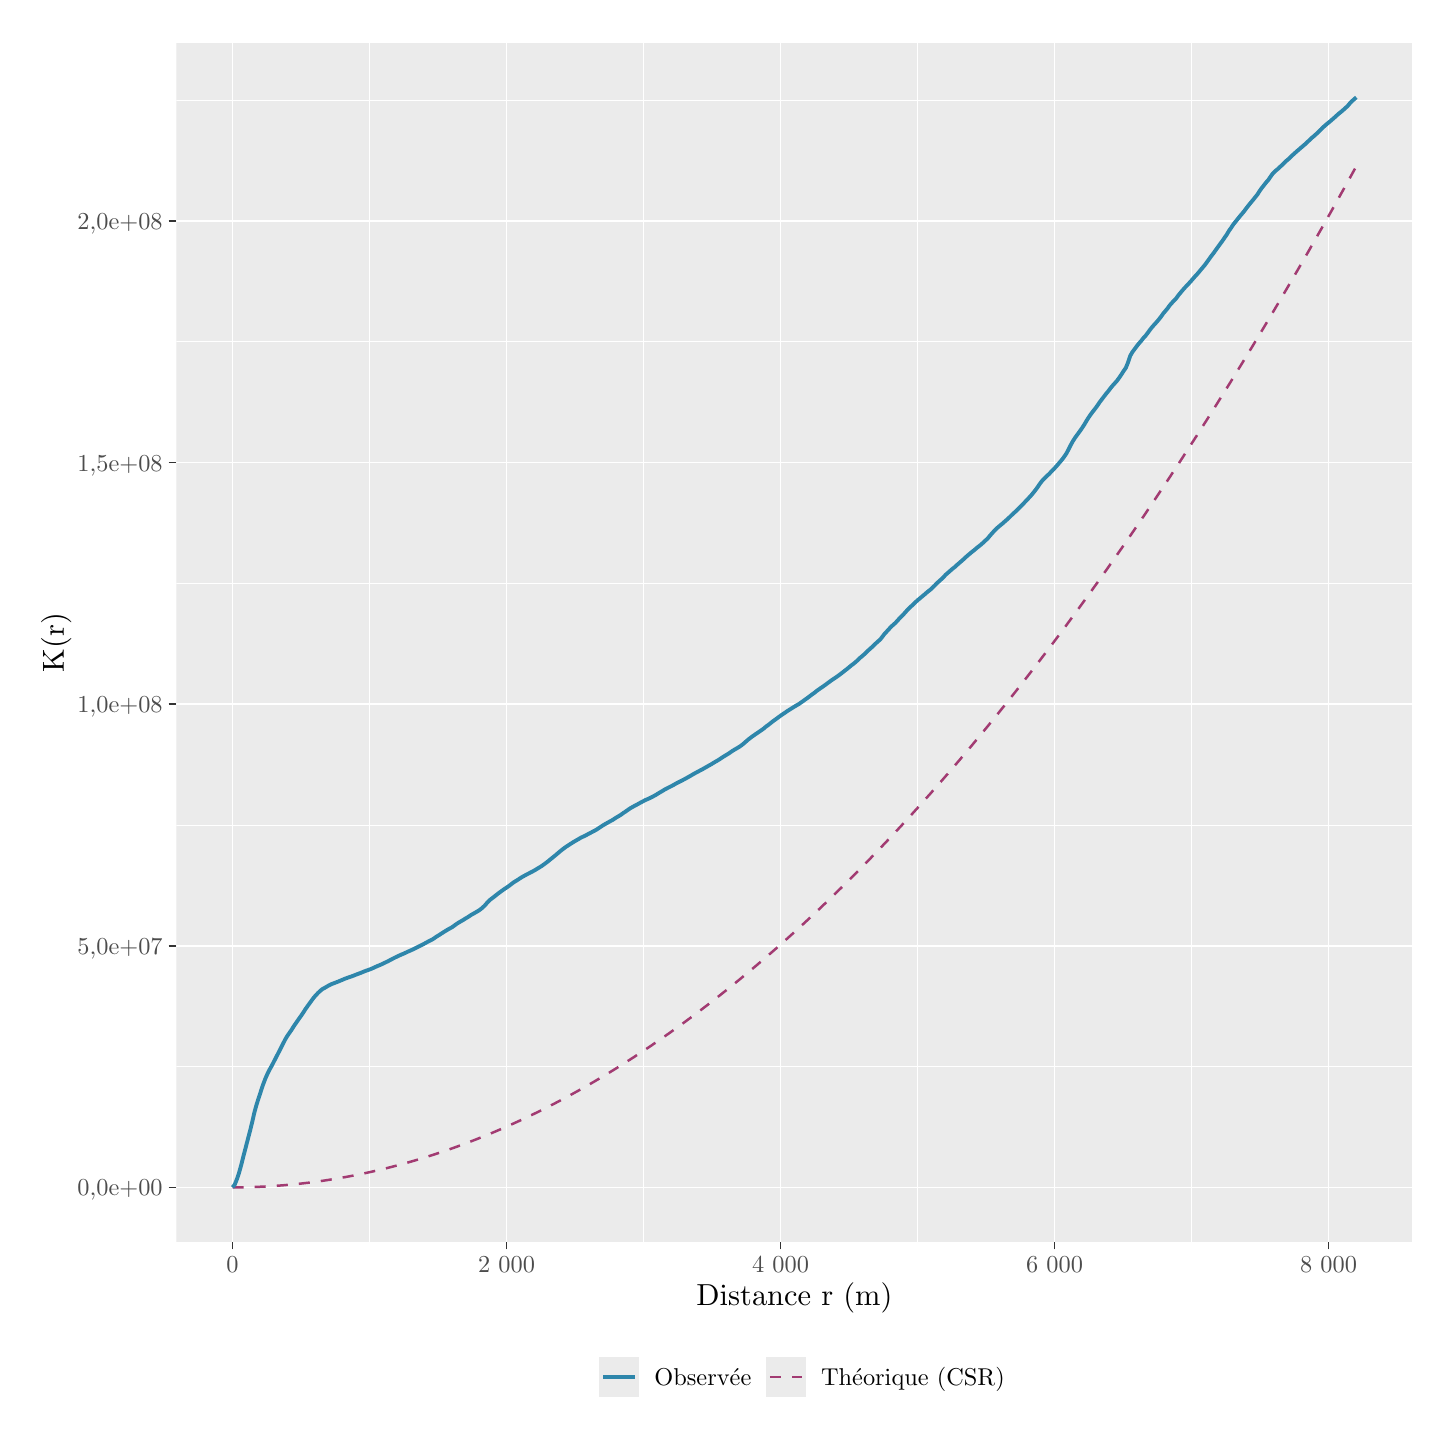
\begin{tikzpicture}[x=1pt,y=1pt]
\definecolor{fillColor}{RGB}{255,255,255}
\path[use as bounding box,fill=fillColor,fill opacity=0.00] (0,0) rectangle (505.89,505.89);
\begin{scope}
\path[clip] (  0.00,  0.00) rectangle (505.89,505.89);
\definecolor{drawColor}{RGB}{255,255,255}
\definecolor{fillColor}{RGB}{255,255,255}

\path[draw=drawColor,line width= 0.6pt,line join=round,line cap=round,fill=fillColor] (  0.00,  0.00) rectangle (505.89,505.89);
\end{scope}
\begin{scope}
\path[clip] ( 53.72, 67.14) rectangle (500.39,500.39);
\definecolor{fillColor}{gray}{0.92}

\path[fill=fillColor] ( 53.72, 67.14) rectangle (500.39,500.39);
\definecolor{drawColor}{RGB}{255,255,255}

\path[draw=drawColor,line width= 0.3pt,line join=round] ( 53.72,130.48) --
	(500.39,130.48);

\path[draw=drawColor,line width= 0.3pt,line join=round] ( 53.72,217.77) --
	(500.39,217.77);

\path[draw=drawColor,line width= 0.3pt,line join=round] ( 53.72,305.06) --
	(500.39,305.06);

\path[draw=drawColor,line width= 0.3pt,line join=round] ( 53.72,392.34) --
	(500.39,392.34);

\path[draw=drawColor,line width= 0.3pt,line join=round] ( 53.72,479.63) --
	(500.39,479.63);

\path[draw=drawColor,line width= 0.3pt,line join=round] (123.53, 67.14) --
	(123.53,500.39);

\path[draw=drawColor,line width= 0.3pt,line join=round] (222.54, 67.14) --
	(222.54,500.39);

\path[draw=drawColor,line width= 0.3pt,line join=round] (321.56, 67.14) --
	(321.56,500.39);

\path[draw=drawColor,line width= 0.3pt,line join=round] (420.58, 67.14) --
	(420.58,500.39);

\path[draw=drawColor,line width= 0.6pt,line join=round] ( 53.72, 86.84) --
	(500.39, 86.84);

\path[draw=drawColor,line width= 0.6pt,line join=round] ( 53.72,174.12) --
	(500.39,174.12);

\path[draw=drawColor,line width= 0.6pt,line join=round] ( 53.72,261.41) --
	(500.39,261.41);

\path[draw=drawColor,line width= 0.6pt,line join=round] ( 53.72,348.70) --
	(500.39,348.70);

\path[draw=drawColor,line width= 0.6pt,line join=round] ( 53.72,435.99) --
	(500.39,435.99);

\path[draw=drawColor,line width= 0.6pt,line join=round] ( 74.02, 67.14) --
	( 74.02,500.39);

\path[draw=drawColor,line width= 0.6pt,line join=round] (173.04, 67.14) --
	(173.04,500.39);

\path[draw=drawColor,line width= 0.6pt,line join=round] (272.05, 67.14) --
	(272.05,500.39);

\path[draw=drawColor,line width= 0.6pt,line join=round] (371.07, 67.14) --
	(371.07,500.39);

\path[draw=drawColor,line width= 0.6pt,line join=round] (470.09, 67.14) --
	(470.09,500.39);
\definecolor{drawColor}{RGB}{162,59,114}

\path[draw=drawColor,line width= 0.9pt,dash pattern=on 4pt off 4pt ,line join=round] ( 74.02, 86.84) --
	( 74.81, 86.84) --
	( 75.61, 86.84) --
	( 76.40, 86.85) --
	( 77.19, 86.86) --
	( 77.99, 86.87) --
	( 78.78, 86.89) --
	( 79.57, 86.91) --
	( 80.37, 86.93) --
	( 81.16, 86.95) --
	( 81.95, 86.98) --
	( 82.74, 87.01) --
	( 83.54, 87.04) --
	( 84.33, 87.07) --
	( 85.12, 87.11) --
	( 85.92, 87.15) --
	( 86.71, 87.20) --
	( 87.50, 87.24) --
	( 88.30, 87.29) --
	( 89.09, 87.34) --
	( 89.88, 87.40) --
	( 90.68, 87.46) --
	( 91.47, 87.52) --
	( 92.26, 87.58) --
	( 93.05, 87.65) --
	( 93.85, 87.72) --
	( 94.64, 87.79) --
	( 95.43, 87.86) --
	( 96.23, 87.94) --
	( 97.02, 88.02) --
	( 97.81, 88.10) --
	( 98.61, 88.19) --
	( 99.40, 88.28) --
	(100.19, 88.37) --
	(100.99, 88.46) --
	(101.78, 88.56) --
	(102.57, 88.66) --
	(103.36, 88.76) --
	(104.16, 88.87) --
	(104.95, 88.98) --
	(105.74, 89.09) --
	(106.54, 89.20) --
	(107.33, 89.32) --
	(108.12, 89.44) --
	(108.92, 89.56) --
	(109.71, 89.69) --
	(110.50, 89.81) --
	(111.30, 89.95) --
	(112.09, 90.08) --
	(112.88, 90.22) --
	(113.68, 90.36) --
	(114.47, 90.50) --
	(115.26, 90.64) --
	(116.05, 90.79) --
	(116.85, 90.94) --
	(117.64, 91.09) --
	(118.43, 91.25) --
	(119.23, 91.41) --
	(120.02, 91.57) --
	(120.81, 91.74) --
	(121.61, 91.90) --
	(122.40, 92.07) --
	(123.19, 92.25) --
	(123.99, 92.42) --
	(124.78, 92.60) --
	(125.57, 92.78) --
	(126.36, 92.97) --
	(127.16, 93.15) --
	(127.95, 93.34) --
	(128.74, 93.54) --
	(129.54, 93.73) --
	(130.33, 93.93) --
	(131.12, 94.13) --
	(131.92, 94.34) --
	(132.71, 94.54) --
	(133.50, 94.75) --
	(134.30, 94.97) --
	(135.09, 95.18) --
	(135.88, 95.40) --
	(136.67, 95.62) --
	(137.47, 95.84) --
	(138.26, 96.07) --
	(139.05, 96.30) --
	(139.85, 96.53) --
	(140.64, 96.77) --
	(141.43, 97.01) --
	(142.23, 97.25) --
	(143.02, 97.49) --
	(143.81, 97.74) --
	(144.61, 97.99) --
	(145.40, 98.24) --
	(146.19, 98.49) --
	(146.99, 98.75) --
	(147.78, 99.01) --
	(148.57, 99.27) --
	(149.36, 99.54) --
	(150.16, 99.81) --
	(150.95,100.08) --
	(151.74,100.35) --
	(152.54,100.63) --
	(153.33,100.91) --
	(154.12,101.19) --
	(154.92,101.48) --
	(155.71,101.77) --
	(156.50,102.06) --
	(157.30,102.35) --
	(158.09,102.65) --
	(158.88,102.95) --
	(159.67,103.25) --
	(160.47,103.56) --
	(161.26,103.87) --
	(162.05,104.18) --
	(162.85,104.49) --
	(163.64,104.81) --
	(164.43,105.13) --
	(165.23,105.45) --
	(166.02,105.78) --
	(166.81,106.10) --
	(167.61,106.43) --
	(168.40,106.77) --
	(169.19,107.10) --
	(169.99,107.44) --
	(170.78,107.79) --
	(171.57,108.13) --
	(172.36,108.48) --
	(173.16,108.83) --
	(173.95,109.18) --
	(174.74,109.54) --
	(175.54,109.90) --
	(176.33,110.26) --
	(177.12,110.62) --
	(177.92,110.99) --
	(178.71,111.36) --
	(179.50,111.73) --
	(180.30,112.11) --
	(181.09,112.49) --
	(181.88,112.87) --
	(182.67,113.25) --
	(183.47,113.64) --
	(184.26,114.03) --
	(185.05,114.42) --
	(185.85,114.82) --
	(186.64,115.22) --
	(187.43,115.62) --
	(188.23,116.02) --
	(189.02,116.43) --
	(189.81,116.84) --
	(190.61,117.25) --
	(191.40,117.67) --
	(192.19,118.08) --
	(192.98,118.50) --
	(193.78,118.93) --
	(194.57,119.35) --
	(195.36,119.78) --
	(196.16,120.22) --
	(196.95,120.65) --
	(197.74,121.09) --
	(198.54,121.53) --
	(199.33,121.97) --
	(200.12,122.42) --
	(200.92,122.87) --
	(201.71,123.32) --
	(202.50,123.77) --
	(203.30,124.23) --
	(204.09,124.69) --
	(204.88,125.15) --
	(205.67,125.62) --
	(206.47,126.09) --
	(207.26,126.56) --
	(208.05,127.03) --
	(208.85,127.51) --
	(209.64,127.99) --
	(210.43,128.47) --
	(211.23,128.96) --
	(212.02,129.45) --
	(212.81,129.94) --
	(213.61,130.43) --
	(214.40,130.93) --
	(215.19,131.43) --
	(215.98,131.93) --
	(216.78,132.44) --
	(217.57,132.95) --
	(218.36,133.46) --
	(219.16,133.97) --
	(219.95,134.49) --
	(220.74,135.01) --
	(221.54,135.53) --
	(222.33,136.05) --
	(223.12,136.58) --
	(223.92,137.11) --
	(224.71,137.65) --
	(225.50,138.18) --
	(226.30,138.72) --
	(227.09,139.26) --
	(227.88,139.81) --
	(228.67,140.35) --
	(229.47,140.91) --
	(230.26,141.46) --
	(231.05,142.01) --
	(231.85,142.57) --
	(232.64,143.13) --
	(233.43,143.70) --
	(234.23,144.27) --
	(235.02,144.84) --
	(235.81,145.41) --
	(236.61,145.98) --
	(237.40,146.56) --
	(238.19,147.14) --
	(238.98,147.73) --
	(239.78,148.32) --
	(240.57,148.91) --
	(241.36,149.50) --
	(242.16,150.09) --
	(242.95,150.69) --
	(243.74,151.29) --
	(244.54,151.90) --
	(245.33,152.50) --
	(246.12,153.11) --
	(246.92,153.72) --
	(247.71,154.34) --
	(248.50,154.96) --
	(249.29,155.58) --
	(250.09,156.20) --
	(250.88,156.83) --
	(251.67,157.46) --
	(252.47,158.09) --
	(253.26,158.72) --
	(254.05,159.36) --
	(254.85,160.00) --
	(255.64,160.64) --
	(256.43,161.29) --
	(257.23,161.94) --
	(258.02,162.59) --
	(258.81,163.25) --
	(259.61,163.90) --
	(260.40,164.56) --
	(261.19,165.23) --
	(261.98,165.89) --
	(262.78,166.56) --
	(263.57,167.23) --
	(264.36,167.91) --
	(265.16,168.58) --
	(265.95,169.26) --
	(266.74,169.94) --
	(267.54,170.63) --
	(268.33,171.32) --
	(269.12,172.01) --
	(269.92,172.70) --
	(270.71,173.40) --
	(271.50,174.10) --
	(272.29,174.80) --
	(273.09,175.51) --
	(273.88,176.22) --
	(274.67,176.93) --
	(275.47,177.64) --
	(276.26,178.36) --
	(277.05,179.08) --
	(277.85,179.80) --
	(278.64,180.52) --
	(279.43,181.25) --
	(280.23,181.98) --
	(281.02,182.71) --
	(281.81,183.45) --
	(282.61,184.19) --
	(283.40,184.93) --
	(284.19,185.67) --
	(284.98,186.42) --
	(285.78,187.17) --
	(286.57,187.93) --
	(287.36,188.68) --
	(288.16,189.44) --
	(288.95,190.20) --
	(289.74,190.97) --
	(290.54,191.73) --
	(291.33,192.50) --
	(292.12,193.27) --
	(292.92,194.05) --
	(293.71,194.83) --
	(294.50,195.61) --
	(295.29,196.39) --
	(296.09,197.18) --
	(296.88,197.97) --
	(297.67,198.76) --
	(298.47,199.56) --
	(299.26,200.36) --
	(300.05,201.16) --
	(300.85,201.96) --
	(301.64,202.77) --
	(302.43,203.58) --
	(303.23,204.39) --
	(304.02,205.20) --
	(304.81,206.02) --
	(305.60,206.84) --
	(306.40,207.66) --
	(307.19,208.49) --
	(307.98,209.32) --
	(308.78,210.15) --
	(309.57,210.99) --
	(310.36,211.82) --
	(311.16,212.66) --
	(311.95,213.51) --
	(312.74,214.35) --
	(313.54,215.20) --
	(314.33,216.05) --
	(315.12,216.91) --
	(315.92,217.76) --
	(316.71,218.62) --
	(317.50,219.49) --
	(318.29,220.35) --
	(319.09,221.22) --
	(319.88,222.09) --
	(320.67,222.97) --
	(321.47,223.84) --
	(322.26,224.72) --
	(323.05,225.61) --
	(323.85,226.49) --
	(324.64,227.38) --
	(325.43,228.27) --
	(326.23,229.16) --
	(327.02,230.06) --
	(327.81,230.96) --
	(328.60,231.86) --
	(329.40,232.77) --
	(330.19,233.67) --
	(330.98,234.58) --
	(331.78,235.50) --
	(332.57,236.41) --
	(333.36,237.33) --
	(334.16,238.26) --
	(334.95,239.18) --
	(335.74,240.11) --
	(336.54,241.04) --
	(337.33,241.97) --
	(338.12,242.91) --
	(338.92,243.85) --
	(339.71,244.79) --
	(340.50,245.73) --
	(341.29,246.68) --
	(342.09,247.63) --
	(342.88,248.58) --
	(343.67,249.54) --
	(344.47,250.50) --
	(345.26,251.46) --
	(346.05,252.42) --
	(346.85,253.39) --
	(347.64,254.36) --
	(348.43,255.33) --
	(349.23,256.31) --
	(350.02,257.28) --
	(350.81,258.26) --
	(351.60,259.25) --
	(352.40,260.24) --
	(353.19,261.22) --
	(353.98,262.22) --
	(354.78,263.21) --
	(355.57,264.21) --
	(356.36,265.21) --
	(357.16,266.21) --
	(357.95,267.22) --
	(358.74,268.23) --
	(359.54,269.24) --
	(360.33,270.26) --
	(361.12,271.27) --
	(361.91,272.29) --
	(362.71,273.32) --
	(363.50,274.34) --
	(364.29,275.37) --
	(365.09,276.40) --
	(365.88,277.44) --
	(366.67,278.48) --
	(367.47,279.52) --
	(368.26,280.56) --
	(369.05,281.60) --
	(369.85,282.65) --
	(370.64,283.70) --
	(371.43,284.76) --
	(372.23,285.82) --
	(373.02,286.88) --
	(373.81,287.94) --
	(374.60,289.00) --
	(375.40,290.07) --
	(376.19,291.14) --
	(376.98,292.22) --
	(377.78,293.29) --
	(378.57,294.37) --
	(379.36,295.46) --
	(380.16,296.54) --
	(380.95,297.63) --
	(381.74,298.72) --
	(382.54,299.81) --
	(383.33,300.91) --
	(384.12,302.01) --
	(384.91,303.11) --
	(385.71,304.22) --
	(386.50,305.32) --
	(387.29,306.43) --
	(388.09,307.55) --
	(388.88,308.66) --
	(389.67,309.78) --
	(390.47,310.90) --
	(391.26,312.03) --
	(392.05,313.16) --
	(392.85,314.29) --
	(393.64,315.42) --
	(394.43,316.55) --
	(395.23,317.69) --
	(396.02,318.83) --
	(396.81,319.98) --
	(397.60,321.13) --
	(398.40,322.28) --
	(399.19,323.43) --
	(399.98,324.58) --
	(400.78,325.74) --
	(401.57,326.90) --
	(402.36,328.07) --
	(403.16,329.23) --
	(403.95,330.40) --
	(404.74,331.58) --
	(405.54,332.75) --
	(406.33,333.93) --
	(407.12,335.11) --
	(407.91,336.29) --
	(408.71,337.48) --
	(409.50,338.67) --
	(410.29,339.86) --
	(411.09,341.06) --
	(411.88,342.25) --
	(412.67,343.45) --
	(413.47,344.66) --
	(414.26,345.86) --
	(415.05,347.07) --
	(415.85,348.29) --
	(416.64,349.50) --
	(417.43,350.72) --
	(418.22,351.94) --
	(419.02,353.16) --
	(419.81,354.39) --
	(420.60,355.62) --
	(421.40,356.85) --
	(422.19,358.08) --
	(422.98,359.32) --
	(423.78,360.56) --
	(424.57,361.80) --
	(425.36,363.05) --
	(426.16,364.29) --
	(426.95,365.55) --
	(427.74,366.80) --
	(428.54,368.06) --
	(429.33,369.32) --
	(430.12,370.58) --
	(430.91,371.84) --
	(431.71,373.11) --
	(432.50,374.38) --
	(433.29,375.66) --
	(434.09,376.93) --
	(434.88,378.21) --
	(435.67,379.50) --
	(436.47,380.78) --
	(437.26,382.07) --
	(438.05,383.36) --
	(438.85,384.65) --
	(439.64,385.95) --
	(440.43,387.25) --
	(441.22,388.55) --
	(442.02,389.85) --
	(442.81,391.16) --
	(443.60,392.47) --
	(444.40,393.78) --
	(445.19,395.10) --
	(445.98,396.42) --
	(446.78,397.74) --
	(447.57,399.07) --
	(448.36,400.39) --
	(449.16,401.72) --
	(449.95,403.06) --
	(450.74,404.39) --
	(451.54,405.73) --
	(452.33,407.07) --
	(453.12,408.42) --
	(453.91,409.76) --
	(454.71,411.11) --
	(455.50,412.46) --
	(456.29,413.82) --
	(457.09,415.18) --
	(457.88,416.54) --
	(458.67,417.90) --
	(459.47,419.27) --
	(460.26,420.64) --
	(461.05,422.01) --
	(461.85,423.39) --
	(462.64,424.76) --
	(463.43,426.14) --
	(464.22,427.53) --
	(465.02,428.91) --
	(465.81,430.30) --
	(466.60,431.70) --
	(467.40,433.09) --
	(468.19,434.49) --
	(468.98,435.89) --
	(469.78,437.29) --
	(470.57,438.70) --
	(471.36,440.11) --
	(472.16,441.52) --
	(472.95,442.93) --
	(473.74,444.35) --
	(474.53,445.77) --
	(475.33,447.19) --
	(476.12,448.62) --
	(476.91,450.05) --
	(477.71,451.48) --
	(478.50,452.91) --
	(479.29,454.35) --
	(480.09,455.79);
\definecolor{drawColor}{RGB}{46,134,171}

\path[draw=drawColor,line width= 1.4pt,line join=round] ( 74.02, 86.84) --
	( 74.81, 87.81) --
	( 75.61, 89.81) --
	( 76.40, 92.18) --
	( 77.19, 95.01) --
	( 77.99, 98.22) --
	( 78.78,101.23) --
	( 79.57,104.28) --
	( 80.37,107.32) --
	( 81.16,110.54) --
	( 81.95,114.02) --
	( 82.74,116.85) --
	( 83.54,119.36) --
	( 84.33,121.76) --
	( 85.12,124.13) --
	( 85.92,126.22) --
	( 86.71,128.00) --
	( 87.50,129.54) --
	( 88.30,130.97) --
	( 89.09,132.51) --
	( 89.88,134.05) --
	( 90.68,135.60) --
	( 91.47,137.12) --
	( 92.26,138.72) --
	( 93.05,140.25) --
	( 93.85,141.61) --
	( 94.64,142.73) --
	( 95.43,143.87) --
	( 96.23,145.18) --
	( 97.02,146.30) --
	( 97.81,147.45) --
	( 98.61,148.57) --
	( 99.40,149.72) --
	(100.19,150.95) --
	(100.99,152.13) --
	(101.78,153.21) --
	(102.57,154.30) --
	(103.36,155.38) --
	(104.16,156.29) --
	(104.95,157.12) --
	(105.74,157.87) --
	(106.54,158.51) --
	(107.33,158.92) --
	(108.12,159.39) --
	(108.92,159.85) --
	(109.71,160.25) --
	(110.50,160.54) --
	(111.30,160.85) --
	(112.09,161.15) --
	(112.88,161.49) --
	(113.68,161.81) --
	(114.47,162.16) --
	(115.26,162.45) --
	(116.05,162.75) --
	(116.85,163.01) --
	(117.64,163.29) --
	(118.43,163.61) --
	(119.23,163.92) --
	(120.02,164.21) --
	(120.81,164.52) --
	(121.61,164.86) --
	(122.40,165.16) --
	(123.19,165.43) --
	(123.99,165.73) --
	(124.78,166.07) --
	(125.57,166.44) --
	(126.36,166.79) --
	(127.16,167.13) --
	(127.95,167.47) --
	(128.74,167.86) --
	(129.54,168.23) --
	(130.33,168.61) --
	(131.12,169.05) --
	(131.92,169.46) --
	(132.71,169.86) --
	(133.50,170.24) --
	(134.30,170.62) --
	(135.09,170.97) --
	(135.88,171.30) --
	(136.67,171.67) --
	(137.47,172.05) --
	(138.26,172.39) --
	(139.05,172.74) --
	(139.85,173.13) --
	(140.64,173.52) --
	(141.43,173.93) --
	(142.23,174.34) --
	(143.02,174.73) --
	(143.81,175.16) --
	(144.61,175.60) --
	(145.40,176.00) --
	(146.19,176.40) --
	(146.99,176.92) --
	(147.78,177.47) --
	(148.57,177.94) --
	(149.36,178.46) --
	(150.16,178.97) --
	(150.95,179.47) --
	(151.74,179.95) --
	(152.54,180.40) --
	(153.33,180.82) --
	(154.12,181.38) --
	(154.92,181.98) --
	(155.71,182.50) --
	(156.50,182.95) --
	(157.30,183.41) --
	(158.09,183.92) --
	(158.88,184.38) --
	(159.67,184.88) --
	(160.47,185.41) --
	(161.26,185.84) --
	(162.05,186.30) --
	(162.85,186.77) --
	(163.64,187.31) --
	(164.43,187.97) --
	(165.23,188.74) --
	(166.02,189.68) --
	(166.81,190.50) --
	(167.61,191.15) --
	(168.40,191.73) --
	(169.19,192.37) --
	(169.99,192.99) --
	(170.78,193.59) --
	(171.57,194.15) --
	(172.36,194.72) --
	(173.16,195.24) --
	(173.95,195.78) --
	(174.74,196.40) --
	(175.54,197.00) --
	(176.33,197.50) --
	(177.12,197.98) --
	(177.92,198.52) --
	(178.71,199.01) --
	(179.50,199.44) --
	(180.30,199.89) --
	(181.09,200.28) --
	(181.88,200.71) --
	(182.67,201.11) --
	(183.47,201.56) --
	(184.26,202.06) --
	(185.05,202.52) --
	(185.85,203.04) --
	(186.64,203.60) --
	(187.43,204.19) --
	(188.23,204.81) --
	(189.02,205.46) --
	(189.81,206.11) --
	(190.61,206.75) --
	(191.40,207.42) --
	(192.19,208.10) --
	(192.98,208.74) --
	(193.78,209.35) --
	(194.57,209.93) --
	(195.36,210.42) --
	(196.16,210.95) --
	(196.95,211.46) --
	(197.74,211.93) --
	(198.54,212.39) --
	(199.33,212.85) --
	(200.12,213.30) --
	(200.92,213.66) --
	(201.71,214.04) --
	(202.50,214.49) --
	(203.30,214.90) --
	(204.09,215.32) --
	(204.88,215.73) --
	(205.67,216.18) --
	(206.47,216.71) --
	(207.26,217.23) --
	(208.05,217.76) --
	(208.85,218.20) --
	(209.64,218.65) --
	(210.43,219.10) --
	(211.23,219.52) --
	(212.02,220.02) --
	(212.81,220.54) --
	(213.61,221.00) --
	(214.40,221.50) --
	(215.19,222.07) --
	(215.98,222.59) --
	(216.78,223.15) --
	(217.57,223.71) --
	(218.36,224.17) --
	(219.16,224.61) --
	(219.95,225.03) --
	(220.74,225.46) --
	(221.54,225.91) --
	(222.33,226.32) --
	(223.12,226.74) --
	(223.92,227.09) --
	(224.71,227.45) --
	(225.50,227.83) --
	(226.30,228.26) --
	(227.09,228.70) --
	(227.88,229.20) --
	(228.67,229.67) --
	(229.47,230.13) --
	(230.26,230.63) --
	(231.05,231.04) --
	(231.85,231.44) --
	(232.64,231.84) --
	(233.43,232.26) --
	(234.23,232.73) --
	(235.02,233.14) --
	(235.81,233.55) --
	(236.61,233.95) --
	(237.40,234.36) --
	(238.19,234.80) --
	(238.98,235.24) --
	(239.78,235.70) --
	(240.57,236.18) --
	(241.36,236.61) --
	(242.16,237.02) --
	(242.95,237.46) --
	(243.74,237.86) --
	(244.54,238.33) --
	(245.33,238.77) --
	(246.12,239.23) --
	(246.92,239.66) --
	(247.71,240.16) --
	(248.50,240.63) --
	(249.29,241.08) --
	(250.09,241.58) --
	(250.88,242.12) --
	(251.67,242.61) --
	(252.47,243.10) --
	(253.26,243.57) --
	(254.05,244.12) --
	(254.85,244.66) --
	(255.64,245.14) --
	(256.43,245.58) --
	(257.23,246.08) --
	(258.02,246.62) --
	(258.81,247.29) --
	(259.61,247.99) --
	(260.40,248.67) --
	(261.19,249.28) --
	(261.98,249.87) --
	(262.78,250.42) --
	(263.57,250.97) --
	(264.36,251.50) --
	(265.16,252.05) --
	(265.95,252.61) --
	(266.74,253.30) --
	(267.54,253.87) --
	(268.33,254.48) --
	(269.12,255.13) --
	(269.92,255.70) --
	(270.71,256.28) --
	(271.50,256.86) --
	(272.29,257.44) --
	(273.09,257.98) --
	(273.88,258.51) --
	(274.67,259.05) --
	(275.47,259.55) --
	(276.26,260.05) --
	(277.05,260.54) --
	(277.85,261.01) --
	(278.64,261.47) --
	(279.43,262.01) --
	(280.23,262.58) --
	(281.02,263.16) --
	(281.81,263.71) --
	(282.61,264.32) --
	(283.40,264.93) --
	(284.19,265.47) --
	(284.98,266.13) --
	(285.78,266.71) --
	(286.57,267.25) --
	(287.36,267.79) --
	(288.16,268.35) --
	(288.95,268.95) --
	(289.74,269.53) --
	(290.54,270.11) --
	(291.33,270.64) --
	(292.12,271.16) --
	(292.92,271.73) --
	(293.71,272.32) --
	(294.50,272.93) --
	(295.29,273.57) --
	(296.09,274.17) --
	(296.88,274.82) --
	(297.67,275.49) --
	(298.47,276.07) --
	(299.26,276.74) --
	(300.05,277.45) --
	(300.85,278.22) --
	(301.64,278.88) --
	(302.43,279.58) --
	(303.23,280.35) --
	(304.02,281.11) --
	(304.81,281.81) --
	(305.60,282.54) --
	(306.40,283.32) --
	(307.19,284.07) --
	(307.98,284.71) --
	(308.78,285.72) --
	(309.57,286.76) --
	(310.36,287.62) --
	(311.16,288.49) --
	(311.95,289.38) --
	(312.74,290.08) --
	(313.54,290.79) --
	(314.33,291.64) --
	(315.12,292.55) --
	(315.92,293.33) --
	(316.71,294.15) --
	(317.50,295.04) --
	(318.29,295.91) --
	(319.09,296.66) --
	(319.88,297.36) --
	(320.67,298.15) --
	(321.47,298.90) --
	(322.26,299.56) --
	(323.05,300.22) --
	(323.85,300.88) --
	(324.64,301.57) --
	(325.43,302.23) --
	(326.23,302.85) --
	(327.02,303.58) --
	(327.81,304.36) --
	(328.60,305.20) --
	(329.40,305.90) --
	(330.19,306.63) --
	(330.98,307.41) --
	(331.78,308.26) --
	(332.57,308.94) --
	(333.36,309.64) --
	(334.16,310.34) --
	(334.95,310.95) --
	(335.74,311.68) --
	(336.54,312.37) --
	(337.33,313.05) --
	(338.12,313.75) --
	(338.92,314.50) --
	(339.71,315.20) --
	(340.50,315.85) --
	(341.29,316.52) --
	(342.09,317.14) --
	(342.88,317.84) --
	(343.67,318.45) --
	(344.47,319.08) --
	(345.26,319.80) --
	(346.05,320.54) --
	(346.85,321.27) --
	(347.64,322.22) --
	(348.43,323.14) --
	(349.23,324.00) --
	(350.02,324.81) --
	(350.81,325.53) --
	(351.60,326.18) --
	(352.40,326.83) --
	(353.19,327.55) --
	(353.98,328.22) --
	(354.78,328.98) --
	(355.57,329.77) --
	(356.36,330.50) --
	(357.16,331.23) --
	(357.95,331.99) --
	(358.74,332.81) --
	(359.54,333.63) --
	(360.33,334.44) --
	(361.12,335.28) --
	(361.91,336.12) --
	(362.71,337.00) --
	(363.50,337.96) --
	(364.29,338.98) --
	(365.09,340.07) --
	(365.88,341.25) --
	(366.67,342.27) --
	(367.47,343.05) --
	(368.26,343.87) --
	(369.05,344.57) --
	(369.85,345.44) --
	(370.64,346.23) --
	(371.43,347.09) --
	(372.23,347.99) --
	(373.02,348.94) --
	(373.81,349.85) --
	(374.60,350.94) --
	(375.40,352.13) --
	(376.19,353.63) --
	(376.98,355.21) --
	(377.78,356.65) --
	(378.57,357.85) --
	(379.36,358.92) --
	(380.16,360.02) --
	(380.95,361.14) --
	(381.74,362.35) --
	(382.54,363.71) --
	(383.33,364.99) --
	(384.12,366.13) --
	(384.91,367.19) --
	(385.71,368.20) --
	(386.50,369.27) --
	(387.29,370.46) --
	(388.09,371.51) --
	(388.88,372.55) --
	(389.67,373.58) --
	(390.47,374.53) --
	(391.26,375.58) --
	(392.05,376.55) --
	(392.85,377.43) --
	(393.64,378.32) --
	(394.43,379.41) --
	(395.23,380.57) --
	(396.02,381.83) --
	(396.81,382.95) --
	(397.60,384.90) --
	(398.40,387.30) --
	(399.19,388.68) --
	(399.98,389.72) --
	(400.78,390.82) --
	(401.57,391.80) --
	(402.36,392.70) --
	(403.16,393.72) --
	(403.95,394.58) --
	(404.74,395.60) --
	(405.54,396.71) --
	(406.33,397.71) --
	(407.12,398.61) --
	(407.91,399.47) --
	(408.71,400.42) --
	(409.50,401.41) --
	(410.29,402.54) --
	(411.09,403.48) --
	(411.88,404.43) --
	(412.67,405.55) --
	(413.47,406.45) --
	(414.26,407.28) --
	(415.05,408.13) --
	(415.85,409.24) --
	(416.64,410.18) --
	(417.43,411.13) --
	(418.22,412.02) --
	(419.02,412.84) --
	(419.81,413.71) --
	(420.60,414.59) --
	(421.40,415.54) --
	(422.19,416.40) --
	(422.98,417.26) --
	(423.78,418.25) --
	(424.57,419.17) --
	(425.36,420.12) --
	(426.16,421.22) --
	(426.95,422.32) --
	(427.74,423.42) --
	(428.54,424.45) --
	(429.33,425.56) --
	(430.12,426.67) --
	(430.91,427.75) --
	(431.71,428.84) --
	(432.50,430.00) --
	(433.29,431.13) --
	(434.09,432.50) --
	(434.88,433.59) --
	(435.67,434.79) --
	(436.47,435.80) --
	(437.26,436.78) --
	(438.05,437.77) --
	(438.85,438.70) --
	(439.64,439.66) --
	(440.43,440.74) --
	(441.22,441.74) --
	(442.02,442.73) --
	(442.81,443.67) --
	(443.60,444.67) --
	(444.40,445.65) --
	(445.19,446.93) --
	(445.98,448.02) --
	(446.78,449.03) --
	(447.57,450.03) --
	(448.36,450.94) --
	(449.16,452.12) --
	(449.95,453.23) --
	(450.74,454.01) --
	(451.54,454.66) --
	(452.33,455.38) --
	(453.12,456.12) --
	(453.91,456.92) --
	(454.71,457.67) --
	(455.50,458.33) --
	(456.29,459.05) --
	(457.09,459.85) --
	(457.88,460.56) --
	(458.67,461.28) --
	(459.47,461.95) --
	(460.26,462.64) --
	(461.05,463.31) --
	(461.85,464.00) --
	(462.64,464.76) --
	(463.43,465.52) --
	(464.22,466.24) --
	(465.02,466.89) --
	(465.81,467.64) --
	(466.60,468.39) --
	(467.40,469.15) --
	(468.19,469.97) --
	(468.98,470.66) --
	(469.78,471.35) --
	(470.57,471.98) --
	(471.36,472.67) --
	(472.16,473.37) --
	(472.95,474.09) --
	(473.74,474.80) --
	(474.53,475.42) --
	(475.33,476.10) --
	(476.12,476.82) --
	(476.91,477.53) --
	(477.71,478.49) --
	(478.50,479.29) --
	(479.29,480.02) --
	(480.09,480.70);
\end{scope}
\begin{scope}
\path[clip] (  0.00,  0.00) rectangle (505.89,505.89);
\definecolor{drawColor}{gray}{0.30}

\node[text=drawColor,anchor=base east,inner sep=0pt, outer sep=0pt, scale=  0.88] at ( 48.77, 83.81) {0,0e+00};

\node[text=drawColor,anchor=base east,inner sep=0pt, outer sep=0pt, scale=  0.88] at ( 48.77,171.09) {5,0e+07};

\node[text=drawColor,anchor=base east,inner sep=0pt, outer sep=0pt, scale=  0.88] at ( 48.77,258.38) {1,0e+08};

\node[text=drawColor,anchor=base east,inner sep=0pt, outer sep=0pt, scale=  0.88] at ( 48.77,345.67) {1,5e+08};

\node[text=drawColor,anchor=base east,inner sep=0pt, outer sep=0pt, scale=  0.88] at ( 48.77,432.96) {2,0e+08};
\end{scope}
\begin{scope}
\path[clip] (  0.00,  0.00) rectangle (505.89,505.89);
\definecolor{drawColor}{gray}{0.20}

\path[draw=drawColor,line width= 0.6pt,line join=round] ( 50.97, 86.84) --
	( 53.72, 86.84);

\path[draw=drawColor,line width= 0.6pt,line join=round] ( 50.97,174.12) --
	( 53.72,174.12);

\path[draw=drawColor,line width= 0.6pt,line join=round] ( 50.97,261.41) --
	( 53.72,261.41);

\path[draw=drawColor,line width= 0.6pt,line join=round] ( 50.97,348.70) --
	( 53.72,348.70);

\path[draw=drawColor,line width= 0.6pt,line join=round] ( 50.97,435.99) --
	( 53.72,435.99);
\end{scope}
\begin{scope}
\path[clip] (  0.00,  0.00) rectangle (505.89,505.89);
\definecolor{drawColor}{gray}{0.20}

\path[draw=drawColor,line width= 0.6pt,line join=round] ( 74.02, 64.39) --
	( 74.02, 67.14);

\path[draw=drawColor,line width= 0.6pt,line join=round] (173.04, 64.39) --
	(173.04, 67.14);

\path[draw=drawColor,line width= 0.6pt,line join=round] (272.05, 64.39) --
	(272.05, 67.14);

\path[draw=drawColor,line width= 0.6pt,line join=round] (371.07, 64.39) --
	(371.07, 67.14);

\path[draw=drawColor,line width= 0.6pt,line join=round] (470.09, 64.39) --
	(470.09, 67.14);
\end{scope}
\begin{scope}
\path[clip] (  0.00,  0.00) rectangle (505.89,505.89);
\definecolor{drawColor}{gray}{0.30}

\node[text=drawColor,anchor=base,inner sep=0pt, outer sep=0pt, scale=  0.88] at ( 74.02, 56.13) {0};

\node[text=drawColor,anchor=base,inner sep=0pt, outer sep=0pt, scale=  0.88] at (173.04, 56.13) {2 000};

\node[text=drawColor,anchor=base,inner sep=0pt, outer sep=0pt, scale=  0.88] at (272.05, 56.13) {4 000};

\node[text=drawColor,anchor=base,inner sep=0pt, outer sep=0pt, scale=  0.88] at (371.07, 56.13) {6 000};

\node[text=drawColor,anchor=base,inner sep=0pt, outer sep=0pt, scale=  0.88] at (470.09, 56.13) {8 000};
\end{scope}
\begin{scope}
\path[clip] (  0.00,  0.00) rectangle (505.89,505.89);
\definecolor{drawColor}{RGB}{0,0,0}

\node[text=drawColor,anchor=base,inner sep=0pt, outer sep=0pt, scale=  1.10] at (277.05, 44.09) {Distance r (m)};
\end{scope}
\begin{scope}
\path[clip] (  0.00,  0.00) rectangle (505.89,505.89);
\definecolor{drawColor}{RGB}{0,0,0}

\node[text=drawColor,rotate= 90.00,anchor=base,inner sep=0pt, outer sep=0pt, scale=  1.10] at ( 13.08,283.77) {K(r)};
\end{scope}
\begin{scope}
\path[clip] (  0.00,  0.00) rectangle (505.89,505.89);
\definecolor{fillColor}{RGB}{255,255,255}

\path[fill=fillColor] (195.51,  5.50) rectangle (358.60, 30.95);
\end{scope}
\begin{scope}
\path[clip] (  0.00,  0.00) rectangle (505.89,505.89);
\definecolor{fillColor}{gray}{0.92}

\path[fill=fillColor] (206.51, 11.00) rectangle (220.97, 25.45);
\definecolor{drawColor}{RGB}{46,134,171}

\path[draw=drawColor,line width= 1.4pt,line join=round] (207.96, 18.23) -- (219.52, 18.23);
\end{scope}
\begin{scope}
\path[clip] (  0.00,  0.00) rectangle (505.89,505.89);
\definecolor{fillColor}{gray}{0.92}

\path[fill=fillColor] (266.75, 11.00) rectangle (281.20, 25.45);
\definecolor{drawColor}{RGB}{162,59,114}

\path[draw=drawColor,line width= 0.9pt,dash pattern=on 4pt off 4pt ,line join=round] (268.20, 18.23) -- (279.76, 18.23);
\end{scope}
\begin{scope}
\path[clip] (  0.00,  0.00) rectangle (505.89,505.89);
\definecolor{drawColor}{RGB}{0,0,0}

\node[text=drawColor,anchor=base west,inner sep=0pt, outer sep=0pt, scale=  0.88] at (226.47, 15.20) {Observée};
\end{scope}
\begin{scope}
\path[clip] (  0.00,  0.00) rectangle (505.89,505.89);
\definecolor{drawColor}{RGB}{0,0,0}

\node[text=drawColor,anchor=base west,inner sep=0pt, outer sep=0pt, scale=  0.88] at (286.70, 15.20) {Théorique (CSR)};
\end{scope}
\end{tikzpicture}
%
        }
    \end{figure}
    \begin{figure}[H]
        \centering
        \caption{Corrélation entre les espèces pour $r \le \SI{1}{\km}$}
        \resize{%
            % Created by tikzDevice version 0.12.6 on 2025-10-11 22:33:34
% !TEX encoding = UTF-8 Unicode
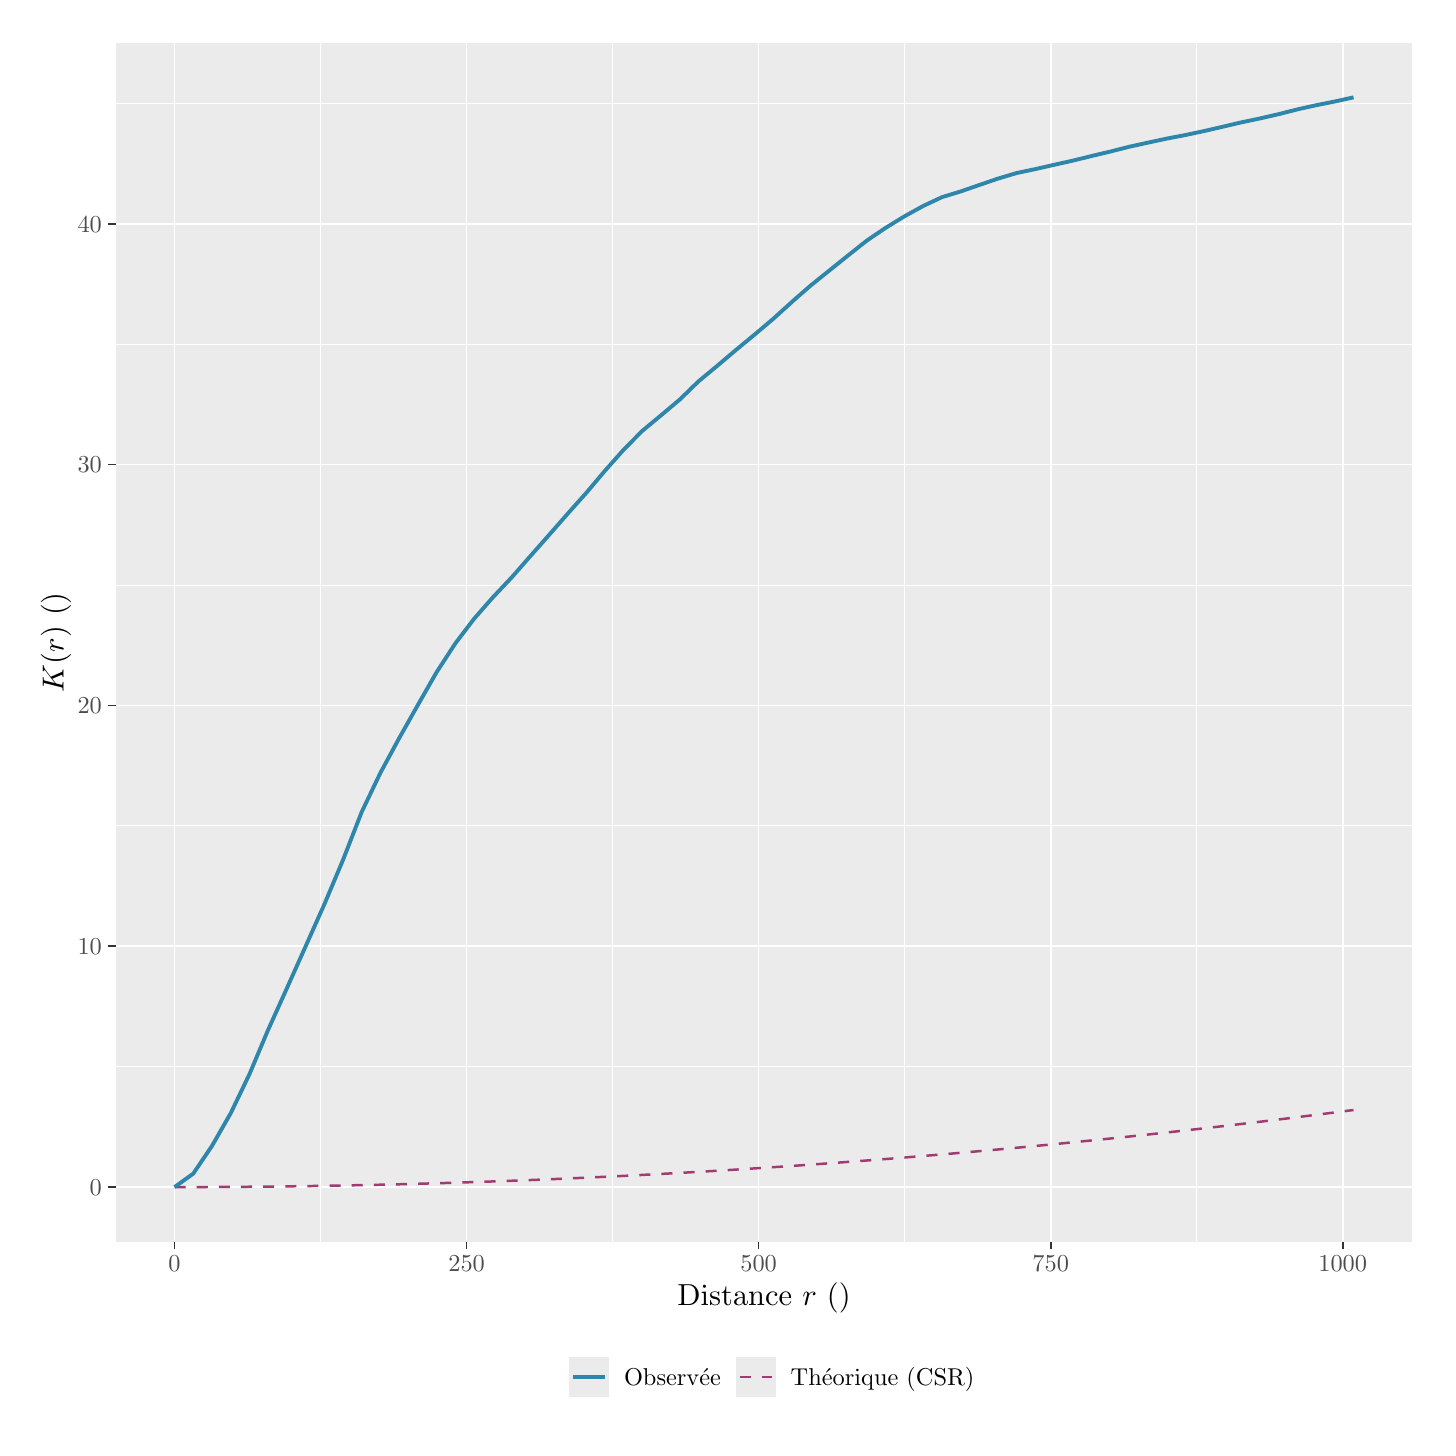
\begin{tikzpicture}[x=1pt,y=1pt]
\definecolor{fillColor}{RGB}{255,255,255}
\path[use as bounding box,fill=fillColor,fill opacity=0.00] (0,0) rectangle (505.89,505.89);
\begin{scope}
\path[clip] (  0.00,  0.00) rectangle (505.89,505.89);
\definecolor{drawColor}{RGB}{255,255,255}
\definecolor{fillColor}{RGB}{255,255,255}

\path[draw=drawColor,line width= 0.6pt,line join=round,line cap=round,fill=fillColor] (  0.00,  0.00) rectangle (505.89,505.89);
\end{scope}
\begin{scope}
\path[clip] ( 31.78, 67.26) rectangle (500.39,500.39);
\definecolor{fillColor}{gray}{0.92}

\path[fill=fillColor] ( 31.78, 67.26) rectangle (500.39,500.39);
\definecolor{drawColor}{RGB}{255,255,255}

\path[draw=drawColor,line width= 0.3pt,line join=round] ( 31.78,130.45) --
	(500.39,130.45);

\path[draw=drawColor,line width= 0.3pt,line join=round] ( 31.78,217.47) --
	(500.39,217.47);

\path[draw=drawColor,line width= 0.3pt,line join=round] ( 31.78,304.48) --
	(500.39,304.48);

\path[draw=drawColor,line width= 0.3pt,line join=round] ( 31.78,391.50) --
	(500.39,391.50);

\path[draw=drawColor,line width= 0.3pt,line join=round] ( 31.78,478.52) --
	(500.39,478.52);

\path[draw=drawColor,line width= 0.3pt,line join=round] (105.84, 67.26) --
	(105.84,500.39);

\path[draw=drawColor,line width= 0.3pt,line join=round] (211.37, 67.26) --
	(211.37,500.39);

\path[draw=drawColor,line width= 0.3pt,line join=round] (316.90, 67.26) --
	(316.90,500.39);

\path[draw=drawColor,line width= 0.3pt,line join=round] (422.43, 67.26) --
	(422.43,500.39);

\path[draw=drawColor,line width= 0.6pt,line join=round] ( 31.78, 86.94) --
	(500.39, 86.94);

\path[draw=drawColor,line width= 0.6pt,line join=round] ( 31.78,173.96) --
	(500.39,173.96);

\path[draw=drawColor,line width= 0.6pt,line join=round] ( 31.78,260.98) --
	(500.39,260.98);

\path[draw=drawColor,line width= 0.6pt,line join=round] ( 31.78,347.99) --
	(500.39,347.99);

\path[draw=drawColor,line width= 0.6pt,line join=round] ( 31.78,435.01) --
	(500.39,435.01);

\path[draw=drawColor,line width= 0.6pt,line join=round] ( 53.08, 67.26) --
	( 53.08,500.39);

\path[draw=drawColor,line width= 0.6pt,line join=round] (158.61, 67.26) --
	(158.61,500.39);

\path[draw=drawColor,line width= 0.6pt,line join=round] (264.14, 67.26) --
	(264.14,500.39);

\path[draw=drawColor,line width= 0.6pt,line join=round] (369.66, 67.26) --
	(369.66,500.39);

\path[draw=drawColor,line width= 0.6pt,line join=round] (475.19, 67.26) --
	(475.19,500.39);
\definecolor{drawColor}{RGB}{162,59,114}

\path[draw=drawColor,line width= 0.9pt,dash pattern=on 4pt off 4pt ,line join=round] ( 53.08, 86.94) --
	( 59.84, 86.95) --
	( 66.60, 86.97) --
	( 73.37, 87.01) --
	( 80.13, 87.06) --
	( 86.89, 87.12) --
	( 93.65, 87.20) --
	(100.41, 87.29) --
	(107.18, 87.39) --
	(113.94, 87.51) --
	(120.70, 87.65) --
	(127.46, 87.79) --
	(134.22, 87.95) --
	(140.99, 88.13) --
	(147.75, 88.32) --
	(154.51, 88.52) --
	(161.27, 88.74) --
	(168.03, 88.97) --
	(174.80, 89.22) --
	(181.56, 89.48) --
	(188.32, 89.75) --
	(195.08, 90.04) --
	(201.84, 90.34) --
	(208.61, 90.66) --
	(215.37, 90.98) --
	(222.13, 91.33) --
	(228.89, 91.69) --
	(235.66, 92.06) --
	(242.42, 92.44) --
	(249.18, 92.84) --
	(255.94, 93.26) --
	(262.70, 93.69) --
	(269.47, 94.13) --
	(276.23, 94.58) --
	(282.99, 95.05) --
	(289.75, 95.54) --
	(296.51, 96.04) --
	(303.28, 96.55) --
	(310.04, 97.07) --
	(316.80, 97.61) --
	(323.56, 98.17) --
	(330.32, 98.74) --
	(337.09, 99.32) --
	(343.85, 99.92) --
	(350.61,100.53) --
	(357.37,101.15) --
	(364.13,101.79) --
	(370.90,102.44) --
	(377.66,103.11) --
	(384.42,103.79) --
	(391.18,104.48) --
	(397.94,105.19) --
	(404.71,105.91) --
	(411.47,106.65) --
	(418.23,107.40) --
	(424.99,108.17) --
	(431.76,108.94) --
	(438.52,109.74) --
	(445.28,110.54) --
	(452.04,111.36) --
	(458.80,112.20) --
	(465.57,113.05) --
	(472.33,113.91) --
	(479.09,114.79);
\definecolor{drawColor}{RGB}{46,134,171}

\path[draw=drawColor,line width= 1.4pt,line join=round] ( 53.08, 86.94) --
	( 59.84, 91.80) --
	( 66.60,101.81) --
	( 73.37,113.63) --
	( 80.13,127.71) --
	( 86.89,143.77) --
	( 93.65,158.74) --
	(100.41,173.88) --
	(107.18,189.06) --
	(113.94,205.14) --
	(120.70,222.48) --
	(127.46,236.62) --
	(134.22,249.12) --
	(140.99,261.13) --
	(147.75,272.96) --
	(154.51,283.36) --
	(161.27,292.24) --
	(168.03,299.96) --
	(174.80,307.13) --
	(181.56,314.83) --
	(188.32,322.48) --
	(195.08,330.20) --
	(201.84,337.77) --
	(208.61,345.79) --
	(215.37,353.41) --
	(222.13,360.22) --
	(228.89,365.83) --
	(235.66,371.53) --
	(242.42,378.10) --
	(249.18,383.70) --
	(255.94,389.43) --
	(262.70,395.00) --
	(269.47,400.73) --
	(276.23,406.85) --
	(282.99,412.76) --
	(289.75,418.19) --
	(296.51,423.62) --
	(303.28,428.99) --
	(310.04,433.56) --
	(316.80,437.70) --
	(323.56,441.44) --
	(330.32,444.62) --
	(337.09,446.69) --
	(343.85,449.03) --
	(350.61,451.34) --
	(357.37,453.36) --
	(364.13,454.78) --
	(370.90,456.33) --
	(377.66,457.83) --
	(384.42,459.51) --
	(391.18,461.11) --
	(397.94,462.83) --
	(404.71,464.32) --
	(411.47,465.77) --
	(418.23,467.07) --
	(424.99,468.50) --
	(431.76,470.07) --
	(438.52,471.66) --
	(445.28,473.08) --
	(452.04,474.63) --
	(458.80,476.35) --
	(465.57,477.86) --
	(472.33,479.21) --
	(479.09,480.70);
\end{scope}
\begin{scope}
\path[clip] (  0.00,  0.00) rectangle (505.89,505.89);
\definecolor{drawColor}{gray}{0.30}

\node[text=drawColor,anchor=base east,inner sep=0pt, outer sep=0pt, scale=  0.88] at ( 26.83, 83.94) {0};

\node[text=drawColor,anchor=base east,inner sep=0pt, outer sep=0pt, scale=  0.88] at ( 26.83,170.95) {10};

\node[text=drawColor,anchor=base east,inner sep=0pt, outer sep=0pt, scale=  0.88] at ( 26.83,257.97) {20};

\node[text=drawColor,anchor=base east,inner sep=0pt, outer sep=0pt, scale=  0.88] at ( 26.83,344.99) {30};

\node[text=drawColor,anchor=base east,inner sep=0pt, outer sep=0pt, scale=  0.88] at ( 26.83,432.00) {40};
\end{scope}
\begin{scope}
\path[clip] (  0.00,  0.00) rectangle (505.89,505.89);
\definecolor{drawColor}{gray}{0.20}

\path[draw=drawColor,line width= 0.6pt,line join=round] ( 29.03, 86.94) --
	( 31.78, 86.94);

\path[draw=drawColor,line width= 0.6pt,line join=round] ( 29.03,173.96) --
	( 31.78,173.96);

\path[draw=drawColor,line width= 0.6pt,line join=round] ( 29.03,260.98) --
	( 31.78,260.98);

\path[draw=drawColor,line width= 0.6pt,line join=round] ( 29.03,347.99) --
	( 31.78,347.99);

\path[draw=drawColor,line width= 0.6pt,line join=round] ( 29.03,435.01) --
	( 31.78,435.01);
\end{scope}
\begin{scope}
\path[clip] (  0.00,  0.00) rectangle (505.89,505.89);
\definecolor{drawColor}{gray}{0.20}

\path[draw=drawColor,line width= 0.6pt,line join=round] ( 53.08, 64.51) --
	( 53.08, 67.26);

\path[draw=drawColor,line width= 0.6pt,line join=round] (158.61, 64.51) --
	(158.61, 67.26);

\path[draw=drawColor,line width= 0.6pt,line join=round] (264.14, 64.51) --
	(264.14, 67.26);

\path[draw=drawColor,line width= 0.6pt,line join=round] (369.66, 64.51) --
	(369.66, 67.26);

\path[draw=drawColor,line width= 0.6pt,line join=round] (475.19, 64.51) --
	(475.19, 67.26);
\end{scope}
\begin{scope}
\path[clip] (  0.00,  0.00) rectangle (505.89,505.89);
\definecolor{drawColor}{gray}{0.30}

\node[text=drawColor,anchor=base,inner sep=0pt, outer sep=0pt, scale=  0.88] at ( 53.08, 56.30) {0};

\node[text=drawColor,anchor=base,inner sep=0pt, outer sep=0pt, scale=  0.88] at (158.61, 56.30) {250};

\node[text=drawColor,anchor=base,inner sep=0pt, outer sep=0pt, scale=  0.88] at (264.14, 56.30) {500};

\node[text=drawColor,anchor=base,inner sep=0pt, outer sep=0pt, scale=  0.88] at (369.66, 56.30) {750};

\node[text=drawColor,anchor=base,inner sep=0pt, outer sep=0pt, scale=  0.88] at (475.19, 56.30) {1000};
\end{scope}
\begin{scope}
\path[clip] (  0.00,  0.00) rectangle (505.89,505.89);
\definecolor{drawColor}{RGB}{0,0,0}

\node[text=drawColor,anchor=base,inner sep=0pt, outer sep=0pt, scale=  1.10] at (266.08, 44.22) {Distance $r$ (\unit{\m})};
\end{scope}
\begin{scope}
\path[clip] (  0.00,  0.00) rectangle (505.89,505.89);
\definecolor{drawColor}{RGB}{0,0,0}

\node[text=drawColor,rotate= 90.00,anchor=base,inner sep=0pt, outer sep=0pt, scale=  1.10] at ( 13.01,283.82) {$K(r)$ (\unit{\km\squared})};
\end{scope}
\begin{scope}
\path[clip] (  0.00,  0.00) rectangle (505.89,505.89);
\definecolor{fillColor}{RGB}{255,255,255}

\path[fill=fillColor] (184.54,  5.50) rectangle (347.63, 30.95);
\end{scope}
\begin{scope}
\path[clip] (  0.00,  0.00) rectangle (505.89,505.89);
\definecolor{fillColor}{gray}{0.92}

\path[fill=fillColor] (195.54, 11.00) rectangle (210.00, 25.45);
\definecolor{drawColor}{RGB}{46,134,171}

\path[draw=drawColor,line width= 1.4pt,line join=round] (196.99, 18.23) -- (208.55, 18.23);
\end{scope}
\begin{scope}
\path[clip] (  0.00,  0.00) rectangle (505.89,505.89);
\definecolor{fillColor}{gray}{0.92}

\path[fill=fillColor] (255.78, 11.00) rectangle (270.23, 25.45);
\definecolor{drawColor}{RGB}{162,59,114}

\path[draw=drawColor,line width= 0.9pt,dash pattern=on 4pt off 4pt ,line join=round] (257.22, 18.23) -- (268.78, 18.23);
\end{scope}
\begin{scope}
\path[clip] (  0.00,  0.00) rectangle (505.89,505.89);
\definecolor{drawColor}{RGB}{0,0,0}

\node[text=drawColor,anchor=base west,inner sep=0pt, outer sep=0pt, scale=  0.88] at (215.50, 15.22) {Observée};
\end{scope}
\begin{scope}
\path[clip] (  0.00,  0.00) rectangle (505.89,505.89);
\definecolor{drawColor}{RGB}{0,0,0}

\node[text=drawColor,anchor=base west,inner sep=0pt, outer sep=0pt, scale=  0.88] at (275.73, 15.22) {Théorique (CSR)};
\end{scope}
\end{tikzpicture}
%
        }
    \end{figure}
    \begin{figure}[H]
        \centering
        \caption{Corrélation normalisée entre les espèces pour $r \ge \SI{50}{\m}$}
        \resize{%
            % Created by tikzDevice version 0.12.6 on 2025-10-15 23:39:35
% !TEX encoding = UTF-8 Unicode
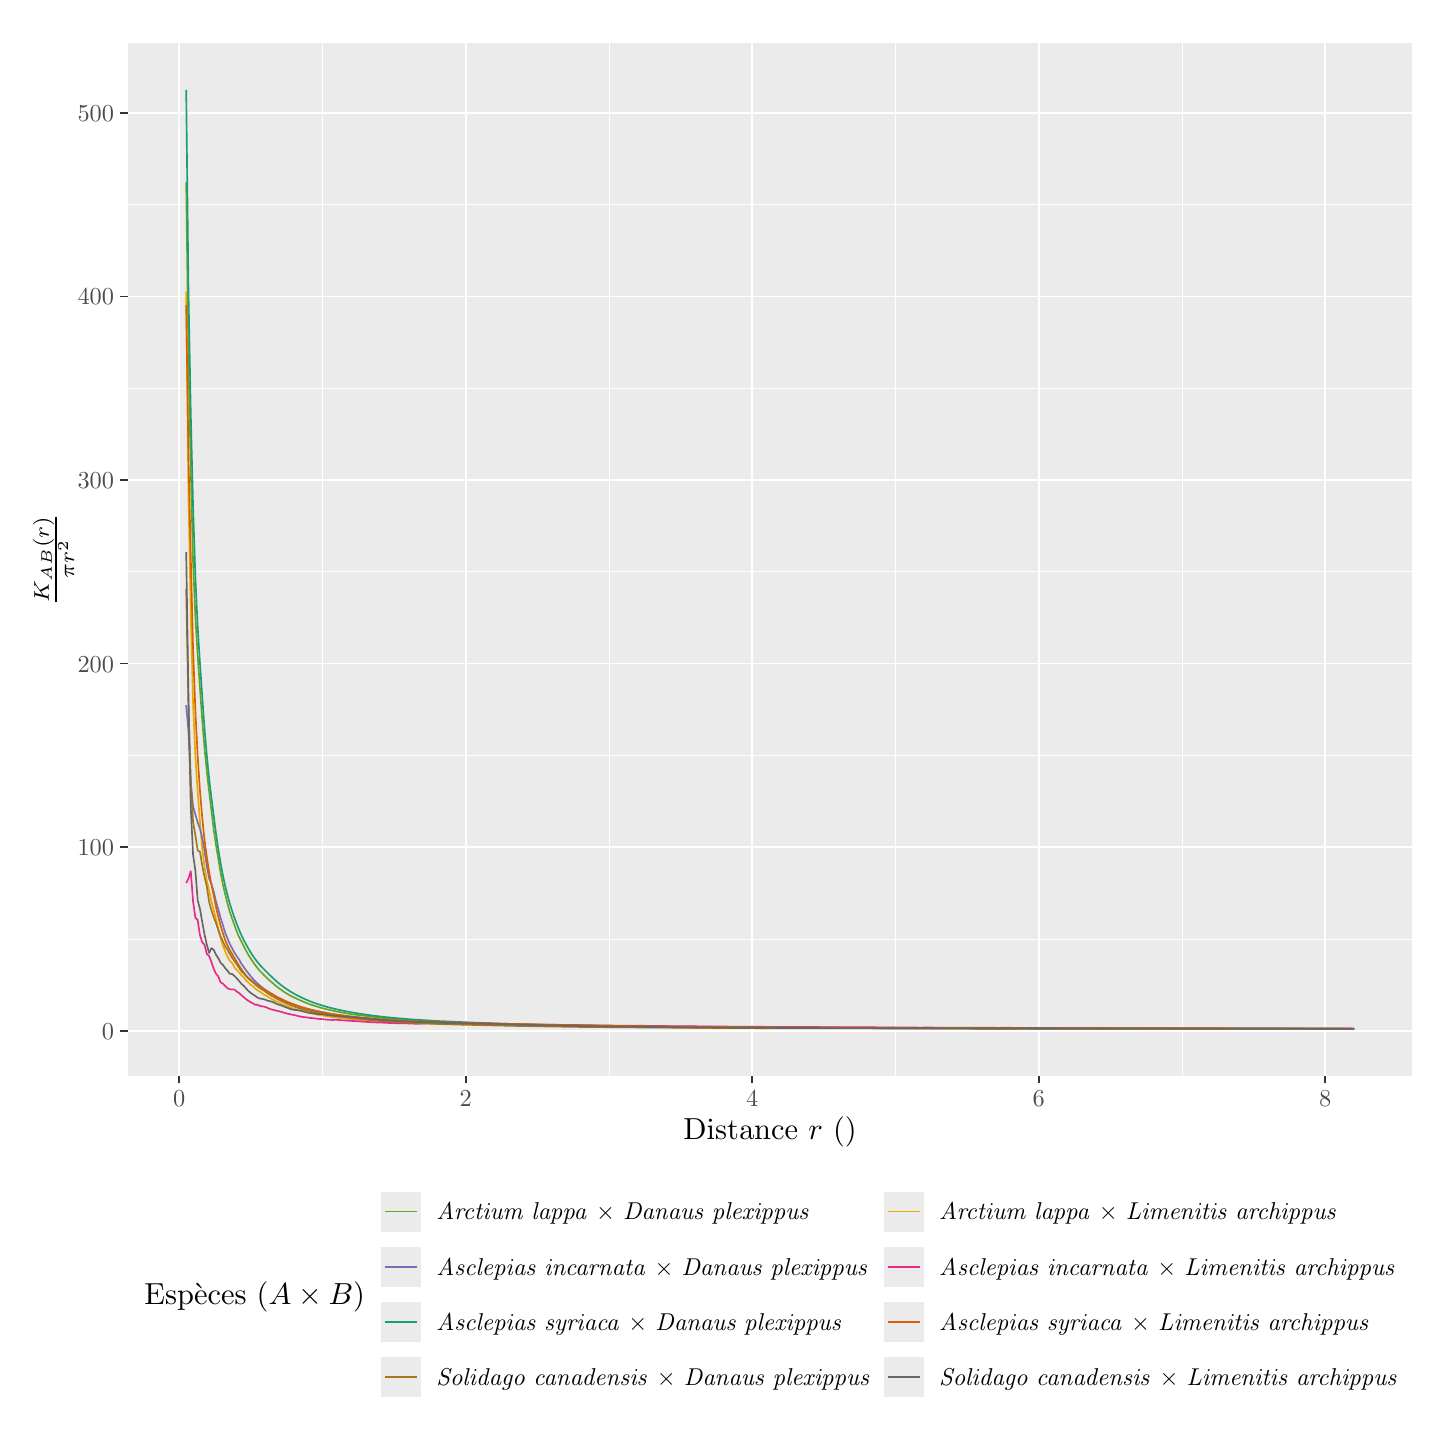
\begin{tikzpicture}[x=1pt,y=1pt]
\definecolor{fillColor}{RGB}{255,255,255}
\path[use as bounding box,fill=fillColor,fill opacity=0.00] (0,0) rectangle (505.89,505.89);
\begin{scope}
\path[clip] (  0.00,  0.00) rectangle (505.89,505.89);
\definecolor{drawColor}{RGB}{255,255,255}
\definecolor{fillColor}{RGB}{255,255,255}

\path[draw=drawColor,line width= 0.6pt,line join=round,line cap=round,fill=fillColor] (  0.00,  0.00) rectangle (505.89,505.89);
\end{scope}
\begin{scope}
\path[clip] ( 36.18,127.12) rectangle (500.39,500.39);
\definecolor{fillColor}{gray}{0.92}

\path[fill=fillColor] ( 36.18,127.12) rectangle (500.39,500.39);
\definecolor{drawColor}{RGB}{255,255,255}

\path[draw=drawColor,line width= 0.3pt,line join=round] ( 36.18,176.53) --
	(500.39,176.53);

\path[draw=drawColor,line width= 0.3pt,line join=round] ( 36.18,242.89) --
	(500.39,242.89);

\path[draw=drawColor,line width= 0.3pt,line join=round] ( 36.18,309.25) --
	(500.39,309.25);

\path[draw=drawColor,line width= 0.3pt,line join=round] ( 36.18,375.61) --
	(500.39,375.61);

\path[draw=drawColor,line width= 0.3pt,line join=round] ( 36.18,441.98) --
	(500.39,441.98);

\path[draw=drawColor,line width= 0.3pt,line join=round] (106.55,127.12) --
	(106.55,500.39);

\path[draw=drawColor,line width= 0.3pt,line join=round] (210.06,127.12) --
	(210.06,500.39);

\path[draw=drawColor,line width= 0.3pt,line join=round] (313.57,127.12) --
	(313.57,500.39);

\path[draw=drawColor,line width= 0.3pt,line join=round] (417.08,127.12) --
	(417.08,500.39);

\path[draw=drawColor,line width= 0.6pt,line join=round] ( 36.18,143.34) --
	(500.39,143.34);

\path[draw=drawColor,line width= 0.6pt,line join=round] ( 36.18,209.71) --
	(500.39,209.71);

\path[draw=drawColor,line width= 0.6pt,line join=round] ( 36.18,276.07) --
	(500.39,276.07);

\path[draw=drawColor,line width= 0.6pt,line join=round] ( 36.18,342.43) --
	(500.39,342.43);

\path[draw=drawColor,line width= 0.6pt,line join=round] ( 36.18,408.80) --
	(500.39,408.80);

\path[draw=drawColor,line width= 0.6pt,line join=round] ( 36.18,475.16) --
	(500.39,475.16);

\path[draw=drawColor,line width= 0.6pt,line join=round] ( 54.79,127.12) --
	( 54.79,500.39);

\path[draw=drawColor,line width= 0.6pt,line join=round] (158.30,127.12) --
	(158.30,500.39);

\path[draw=drawColor,line width= 0.6pt,line join=round] (261.81,127.12) --
	(261.81,500.39);

\path[draw=drawColor,line width= 0.6pt,line join=round] (365.32,127.12) --
	(365.32,500.39);

\path[draw=drawColor,line width= 0.6pt,line join=round] (468.83,127.12) --
	(468.83,500.39);
\definecolor{drawColor}{RGB}{102,166,30}

\path[draw=drawColor,line width= 0.6pt,line join=round] ( 57.28,450.11) --
	( 58.11,385.62) --
	( 58.94,345.78) --
	( 59.77,312.64) --
	( 60.60,292.86) --
	( 61.43,279.02) --
	( 62.25,267.35) --
	( 63.08,255.63) --
	( 63.91,245.51) --
	( 64.74,237.11) --
	( 65.57,229.84) --
	( 66.40,223.07) --
	( 67.23,216.01) --
	( 68.06,210.46) --
	( 68.89,205.55) --
	( 69.72,200.53) --
	( 70.55,196.24) --
	( 71.37,192.73) --
	( 72.20,189.40) --
	( 73.03,186.39) --
	( 73.86,184.03) --
	( 74.69,181.68) --
	( 75.52,179.39) --
	( 76.35,177.39) --
	( 77.18,175.73) --
	( 78.01,174.06) --
	( 78.84,172.49) --
	( 79.67,171.00) --
	( 80.49,169.69) --
	( 81.32,168.44) --
	( 82.15,167.25) --
	( 82.98,166.15) --
	( 83.81,165.18) --
	( 84.64,164.31) --
	( 85.47,163.46) --
	( 86.30,162.67) --
	( 87.13,161.86) --
	( 87.96,161.13) --
	( 88.79,160.44) --
	( 89.61,159.71) --
	( 90.44,159.07) --
	( 91.27,158.44) --
	( 92.10,157.85) --
	( 92.93,157.31) --
	( 93.76,156.80) --
	( 94.59,156.29) --
	( 95.42,155.86) --
	( 96.25,155.45) --
	( 97.08,155.06) --
	( 97.91,154.67) --
	( 98.73,154.29) --
	( 99.56,153.94) --
	(100.39,153.60) --
	(101.22,153.27) --
	(102.05,152.96) --
	(102.88,152.68) --
	(103.71,152.42) --
	(104.54,152.17) --
	(105.37,151.92) --
	(106.20,151.67) --
	(107.03,151.45) --
	(107.85,151.24) --
	(108.68,151.04) --
	(109.51,150.84) --
	(110.34,150.65) --
	(111.17,150.48) --
	(112.00,150.31) --
	(112.83,150.16) --
	(113.66,150.00) --
	(114.49,149.86) --
	(115.32,149.70) --
	(116.15,149.57) --
	(116.97,149.43) --
	(117.80,149.33) --
	(118.63,149.22) --
	(119.46,149.11) --
	(120.29,149.00) --
	(121.12,148.92) --
	(121.95,148.81) --
	(122.78,148.70) --
	(123.61,148.60) --
	(124.44,148.50) --
	(125.27,148.40) --
	(126.09,148.31) --
	(126.92,148.21) --
	(127.75,148.12) --
	(128.58,148.04) --
	(129.41,147.96) --
	(130.24,147.88) --
	(131.07,147.81) --
	(131.90,147.75) --
	(132.73,147.68) --
	(133.56,147.61) --
	(134.39,147.54) --
	(135.21,147.47) --
	(136.04,147.40) --
	(136.87,147.35) --
	(137.70,147.29) --
	(138.53,147.23) --
	(139.36,147.17) --
	(140.19,147.12) --
	(141.02,147.07) --
	(141.85,147.02) --
	(142.68,146.97) --
	(143.51,146.92) --
	(144.33,146.87) --
	(145.16,146.82) --
	(145.99,146.77) --
	(146.82,146.72) --
	(147.65,146.67) --
	(148.48,146.63) --
	(149.31,146.59) --
	(150.14,146.55) --
	(150.97,146.52) --
	(151.80,146.49) --
	(152.63,146.45) --
	(153.45,146.41) --
	(154.28,146.38) --
	(155.11,146.36) --
	(155.94,146.32) --
	(156.77,146.29) --
	(157.60,146.25) --
	(158.43,146.22) --
	(159.26,146.19) --
	(160.09,146.15) --
	(160.92,146.13) --
	(161.75,146.10) --
	(162.57,146.07) --
	(163.40,146.04) --
	(164.23,146.01) --
	(165.06,145.98) --
	(165.89,145.95) --
	(166.72,145.92) --
	(167.55,145.89) --
	(168.38,145.86) --
	(169.21,145.83) --
	(170.04,145.81) --
	(170.87,145.78) --
	(171.69,145.75) --
	(172.52,145.73) --
	(173.35,145.70) --
	(174.18,145.68) --
	(175.01,145.66) --
	(175.84,145.64) --
	(176.67,145.62) --
	(177.50,145.60) --
	(178.33,145.58) --
	(179.16,145.55) --
	(179.99,145.53) --
	(180.81,145.51) --
	(181.64,145.49) --
	(182.47,145.47) --
	(183.30,145.45) --
	(184.13,145.43) --
	(184.96,145.41) --
	(185.79,145.39) --
	(186.62,145.37) --
	(187.45,145.36) --
	(188.28,145.34) --
	(189.11,145.32) --
	(189.93,145.30) --
	(190.76,145.29) --
	(191.59,145.27) --
	(192.42,145.25) --
	(193.25,145.24) --
	(194.08,145.22) --
	(194.91,145.21) --
	(195.74,145.19) --
	(196.57,145.18) --
	(197.40,145.17) --
	(198.23,145.15) --
	(199.06,145.14) --
	(199.88,145.12) --
	(200.71,145.11) --
	(201.54,145.10) --
	(202.37,145.09) --
	(203.20,145.08) --
	(204.03,145.07) --
	(204.86,145.06) --
	(205.69,145.04) --
	(206.52,145.04) --
	(207.35,145.02) --
	(208.18,145.01) --
	(209.00,145.00) --
	(209.83,144.99) --
	(210.66,144.98) --
	(211.49,144.97) --
	(212.32,144.96) --
	(213.15,144.95) --
	(213.98,144.94) --
	(214.81,144.93) --
	(215.64,144.92) --
	(216.47,144.91) --
	(217.30,144.90) --
	(218.12,144.89) --
	(218.95,144.88) --
	(219.78,144.87) --
	(220.61,144.86) --
	(221.44,144.85) --
	(222.27,144.84) --
	(223.10,144.83) --
	(223.93,144.82) --
	(224.76,144.82) --
	(225.59,144.81) --
	(226.42,144.80) --
	(227.24,144.79) --
	(228.07,144.79) --
	(228.90,144.78) --
	(229.73,144.78) --
	(230.56,144.77) --
	(231.39,144.76) --
	(232.22,144.75) --
	(233.05,144.75) --
	(233.88,144.74) --
	(234.71,144.73) --
	(235.54,144.72) --
	(236.36,144.72) --
	(237.19,144.71) --
	(238.02,144.70) --
	(238.85,144.70) --
	(239.68,144.69) --
	(240.51,144.69) --
	(241.34,144.69) --
	(242.17,144.68) --
	(243.00,144.67) --
	(243.83,144.67) --
	(244.66,144.66) --
	(245.48,144.65) --
	(246.31,144.65) --
	(247.14,144.64) --
	(247.97,144.64) --
	(248.80,144.64) --
	(249.63,144.63) --
	(250.46,144.63) --
	(251.29,144.62) --
	(252.12,144.61) --
	(252.95,144.61) --
	(253.78,144.61) --
	(254.60,144.60) --
	(255.43,144.60) --
	(256.26,144.59) --
	(257.09,144.59) --
	(257.92,144.58) --
	(258.75,144.58) --
	(259.58,144.58) --
	(260.41,144.57) --
	(261.24,144.57) --
	(262.07,144.56) --
	(262.90,144.56) --
	(263.72,144.55) --
	(264.55,144.55) --
	(265.38,144.54) --
	(266.21,144.54) --
	(267.04,144.53) --
	(267.87,144.53) --
	(268.70,144.52) --
	(269.53,144.52) --
	(270.36,144.51) --
	(271.19,144.51) --
	(272.02,144.50) --
	(272.84,144.50) --
	(273.67,144.49) --
	(274.50,144.49) --
	(275.33,144.49) --
	(276.16,144.48) --
	(276.99,144.48) --
	(277.82,144.48) --
	(278.65,144.47) --
	(279.48,144.47) --
	(280.31,144.46) --
	(281.14,144.46) --
	(281.96,144.45) --
	(282.79,144.45) --
	(283.62,144.45) --
	(284.45,144.44) --
	(285.28,144.44) --
	(286.11,144.44) --
	(286.94,144.43) --
	(287.77,144.43) --
	(288.60,144.43) --
	(289.43,144.43) --
	(290.26,144.42) --
	(291.08,144.42) --
	(291.91,144.42) --
	(292.74,144.41) --
	(293.57,144.41) --
	(294.40,144.40) --
	(295.23,144.40) --
	(296.06,144.40) --
	(296.89,144.40) --
	(297.72,144.39) --
	(298.55,144.39) --
	(299.38,144.39) --
	(300.20,144.38) --
	(301.03,144.38) --
	(301.86,144.38) --
	(302.69,144.38) --
	(303.52,144.37) --
	(304.35,144.37) --
	(305.18,144.37) --
	(306.01,144.37) --
	(306.84,144.37) --
	(307.67,144.36) --
	(308.50,144.36) --
	(309.32,144.36) --
	(310.15,144.36) --
	(310.98,144.36) --
	(311.81,144.35) --
	(312.64,144.35) --
	(313.47,144.35) --
	(314.30,144.34) --
	(315.13,144.34) --
	(315.96,144.34) --
	(316.79,144.34) --
	(317.62,144.33) --
	(318.44,144.33) --
	(319.27,144.33) --
	(320.10,144.32) --
	(320.93,144.32) --
	(321.76,144.32) --
	(322.59,144.32) --
	(323.42,144.32) --
	(324.25,144.32) --
	(325.08,144.31) --
	(325.91,144.31) --
	(326.74,144.31) --
	(327.56,144.31) --
	(328.39,144.31) --
	(329.22,144.31) --
	(330.05,144.30) --
	(330.88,144.30) --
	(331.71,144.30) --
	(332.54,144.30) --
	(333.37,144.29) --
	(334.20,144.29) --
	(335.03,144.29) --
	(335.86,144.29) --
	(336.68,144.29) --
	(337.51,144.28) --
	(338.34,144.28) --
	(339.17,144.28) --
	(340.00,144.27) --
	(340.83,144.27) --
	(341.66,144.27) --
	(342.49,144.27) --
	(343.32,144.27) --
	(344.15,144.26) --
	(344.98,144.26) --
	(345.81,144.26) --
	(346.63,144.26) --
	(347.46,144.25) --
	(348.29,144.25) --
	(349.12,144.25) --
	(349.95,144.25) --
	(350.78,144.25) --
	(351.61,144.24) --
	(352.44,144.24) --
	(353.27,144.24) --
	(354.10,144.24) --
	(354.93,144.24) --
	(355.75,144.24) --
	(356.58,144.24) --
	(357.41,144.24) --
	(358.24,144.24) --
	(359.07,144.24) --
	(359.90,144.24) --
	(360.73,144.24) --
	(361.56,144.24) --
	(362.39,144.24) --
	(363.22,144.23) --
	(364.05,144.23) --
	(364.87,144.23) --
	(365.70,144.23) --
	(366.53,144.23) --
	(367.36,144.23) --
	(368.19,144.23) --
	(369.02,144.22) --
	(369.85,144.22) --
	(370.68,144.22) --
	(371.51,144.22) --
	(372.34,144.22) --
	(373.17,144.22) --
	(373.99,144.22) --
	(374.82,144.21) --
	(375.65,144.21) --
	(376.48,144.21) --
	(377.31,144.21) --
	(378.14,144.21) --
	(378.97,144.21) --
	(379.80,144.21) --
	(380.63,144.21) --
	(381.46,144.21) --
	(382.29,144.21) --
	(383.11,144.21) --
	(383.94,144.21) --
	(384.77,144.21) --
	(385.60,144.20) --
	(386.43,144.20) --
	(387.26,144.20) --
	(388.09,144.20) --
	(388.92,144.20) --
	(389.75,144.20) --
	(390.58,144.20) --
	(391.41,144.20) --
	(392.23,144.20) --
	(393.06,144.20) --
	(393.89,144.20) --
	(394.72,144.20) --
	(395.55,144.20) --
	(396.38,144.19) --
	(397.21,144.19) --
	(398.04,144.19) --
	(398.87,144.19) --
	(399.70,144.19) --
	(400.53,144.19) --
	(401.35,144.19) --
	(402.18,144.19) --
	(403.01,144.19) --
	(403.84,144.18) --
	(404.67,144.18) --
	(405.50,144.18) --
	(406.33,144.18) --
	(407.16,144.18) --
	(407.99,144.18) --
	(408.82,144.18) --
	(409.65,144.18) --
	(410.47,144.18) --
	(411.30,144.18) --
	(412.13,144.18) --
	(412.96,144.17) --
	(413.79,144.17) --
	(414.62,144.17) --
	(415.45,144.17) --
	(416.28,144.17) --
	(417.11,144.17) --
	(417.94,144.17) --
	(418.77,144.17) --
	(419.59,144.17) --
	(420.42,144.17) --
	(421.25,144.16) --
	(422.08,144.16) --
	(422.91,144.16) --
	(423.74,144.16) --
	(424.57,144.16) --
	(425.40,144.16) --
	(426.23,144.16) --
	(427.06,144.16) --
	(427.89,144.16) --
	(428.71,144.16) --
	(429.54,144.16) --
	(430.37,144.16) --
	(431.20,144.16) --
	(432.03,144.16) --
	(432.86,144.15) --
	(433.69,144.15) --
	(434.52,144.15) --
	(435.35,144.15) --
	(436.18,144.15) --
	(437.01,144.15) --
	(437.83,144.15) --
	(438.66,144.15) --
	(439.49,144.15) --
	(440.32,144.15) --
	(441.15,144.15) --
	(441.98,144.15) --
	(442.81,144.15) --
	(443.64,144.15) --
	(444.47,144.14) --
	(445.30,144.14) --
	(446.13,144.14) --
	(446.95,144.14) --
	(447.78,144.14) --
	(448.61,144.14) --
	(449.44,144.14) --
	(450.27,144.14) --
	(451.10,144.14) --
	(451.93,144.13) --
	(452.76,144.13) --
	(453.59,144.13) --
	(454.42,144.13) --
	(455.25,144.13) --
	(456.07,144.13) --
	(456.90,144.12) --
	(457.73,144.12) --
	(458.56,144.12) --
	(459.39,144.12) --
	(460.22,144.12) --
	(461.05,144.12) --
	(461.88,144.11) --
	(462.71,144.11) --
	(463.54,144.11) --
	(464.37,144.11) --
	(465.19,144.11) --
	(466.02,144.11) --
	(466.85,144.10) --
	(467.68,144.10) --
	(468.51,144.10) --
	(469.34,144.10) --
	(470.17,144.10) --
	(471.00,144.10) --
	(471.83,144.10) --
	(472.66,144.09) --
	(473.49,144.09) --
	(474.31,144.09) --
	(475.14,144.09) --
	(475.97,144.09) --
	(476.80,144.09) --
	(477.63,144.09) --
	(478.46,144.09) --
	(479.29,144.09);
\definecolor{drawColor}{RGB}{230,171,2}

\path[draw=drawColor,line width= 0.6pt,line join=round] ( 57.28,410.57) --
	( 58.11,336.25) --
	( 58.94,294.06) --
	( 59.77,261.37) --
	( 60.60,242.33) --
	( 61.43,229.78) --
	( 62.25,219.06) --
	( 63.08,209.08) --
	( 63.91,202.64) --
	( 64.74,197.62) --
	( 65.57,194.10) --
	( 66.40,190.18) --
	( 67.23,186.99) --
	( 68.06,183.74) --
	( 68.89,180.24) --
	( 69.72,176.87) --
	( 70.55,174.21) --
	( 71.37,172.10) --
	( 72.20,170.16) --
	( 73.03,168.69) --
	( 73.86,167.97) --
	( 74.69,166.38) --
	( 75.52,165.41) --
	( 76.35,164.57) --
	( 77.18,163.52) --
	( 78.01,162.77) --
	( 78.84,161.65) --
	( 79.67,160.89) --
	( 80.49,160.07) --
	( 81.32,159.59) --
	( 82.15,158.73) --
	( 82.98,158.12) --
	( 83.81,157.64) --
	( 84.64,157.08) --
	( 85.47,156.40) --
	( 86.30,156.06) --
	( 87.13,155.52) --
	( 87.96,155.07) --
	( 88.79,154.60) --
	( 89.61,154.14) --
	( 90.44,153.75) --
	( 91.27,153.37) --
	( 92.10,152.96) --
	( 92.93,152.59) --
	( 93.76,152.25) --
	( 94.59,151.97) --
	( 95.42,151.64) --
	( 96.25,151.36) --
	( 97.08,151.08) --
	( 97.91,150.86) --
	( 98.73,150.61) --
	( 99.56,150.38) --
	(100.39,150.21) --
	(101.22,149.99) --
	(102.05,149.81) --
	(102.88,149.62) --
	(103.71,149.45) --
	(104.54,149.27) --
	(105.37,149.13) --
	(106.20,148.97) --
	(107.03,148.83) --
	(107.85,148.70) --
	(108.68,148.56) --
	(109.51,148.44) --
	(110.34,148.35) --
	(111.17,148.23) --
	(112.00,148.10) --
	(112.83,148.02) --
	(113.66,147.92) --
	(114.49,147.81) --
	(115.32,147.73) --
	(116.15,147.62) --
	(116.97,147.56) --
	(117.80,147.48) --
	(118.63,147.44) --
	(119.46,147.38) --
	(120.29,147.34) --
	(121.12,147.29) --
	(121.95,147.22) --
	(122.78,147.20) --
	(123.61,147.15) --
	(124.44,147.08) --
	(125.27,147.02) --
	(126.09,146.95) --
	(126.92,146.89) --
	(127.75,146.82) --
	(128.58,146.77) --
	(129.41,146.72) --
	(130.24,146.67) --
	(131.07,146.62) --
	(131.90,146.57) --
	(132.73,146.53) --
	(133.56,146.50) --
	(134.39,146.45) --
	(135.21,146.42) --
	(136.04,146.39) --
	(136.87,146.37) --
	(137.70,146.32) --
	(138.53,146.28) --
	(139.36,146.24) --
	(140.19,146.21) --
	(141.02,146.18) --
	(141.85,146.16) --
	(142.68,146.14) --
	(143.51,146.11) --
	(144.33,146.09) --
	(145.16,146.07) --
	(145.99,146.04) --
	(146.82,146.01) --
	(147.65,145.98) --
	(148.48,145.94) --
	(149.31,145.91) --
	(150.14,145.89) --
	(150.97,145.87) --
	(151.80,145.84) --
	(152.63,145.84) --
	(153.45,145.83) --
	(154.28,145.83) --
	(155.11,145.83) --
	(155.94,145.82) --
	(156.77,145.80) --
	(157.60,145.78) --
	(158.43,145.77) --
	(159.26,145.75) --
	(160.09,145.74) --
	(160.92,145.73) --
	(161.75,145.71) --
	(162.57,145.69) --
	(163.40,145.68) --
	(164.23,145.66) --
	(165.06,145.63) --
	(165.89,145.61) --
	(166.72,145.58) --
	(167.55,145.56) --
	(168.38,145.54) --
	(169.21,145.52) --
	(170.04,145.51) --
	(170.87,145.48) --
	(171.69,145.46) --
	(172.52,145.44) --
	(173.35,145.42) --
	(174.18,145.40) --
	(175.01,145.39) --
	(175.84,145.39) --
	(176.67,145.38) --
	(177.50,145.36) --
	(178.33,145.36) --
	(179.16,145.34) --
	(179.99,145.32) --
	(180.81,145.32) --
	(181.64,145.30) --
	(182.47,145.29) --
	(183.30,145.28) --
	(184.13,145.28) --
	(184.96,145.26) --
	(185.79,145.25) --
	(186.62,145.23) --
	(187.45,145.21) --
	(188.28,145.20) --
	(189.11,145.18) --
	(189.93,145.17) --
	(190.76,145.16) --
	(191.59,145.14) --
	(192.42,145.13) --
	(193.25,145.12) --
	(194.08,145.10) --
	(194.91,145.09) --
	(195.74,145.08) --
	(196.57,145.07) --
	(197.40,145.05) --
	(198.23,145.03) --
	(199.06,145.02) --
	(199.88,145.00) --
	(200.71,144.99) --
	(201.54,144.99) --
	(202.37,144.99) --
	(203.20,144.98) --
	(204.03,144.96) --
	(204.86,144.95) --
	(205.69,144.95) --
	(206.52,144.94) --
	(207.35,144.93) --
	(208.18,144.92) --
	(209.00,144.92) --
	(209.83,144.91) --
	(210.66,144.90) --
	(211.49,144.89) --
	(212.32,144.89) --
	(213.15,144.88) --
	(213.98,144.86) --
	(214.81,144.85) --
	(215.64,144.84) --
	(216.47,144.83) --
	(217.30,144.82) --
	(218.12,144.81) --
	(218.95,144.80) --
	(219.78,144.79) --
	(220.61,144.78) --
	(221.44,144.77) --
	(222.27,144.76) --
	(223.10,144.75) --
	(223.93,144.74) --
	(224.76,144.74) --
	(225.59,144.73) --
	(226.42,144.72) --
	(227.24,144.71) --
	(228.07,144.71) --
	(228.90,144.71) --
	(229.73,144.70) --
	(230.56,144.69) --
	(231.39,144.69) --
	(232.22,144.68) --
	(233.05,144.67) --
	(233.88,144.67) --
	(234.71,144.66) --
	(235.54,144.65) --
	(236.36,144.65) --
	(237.19,144.64) --
	(238.02,144.63) --
	(238.85,144.63) --
	(239.68,144.62) --
	(240.51,144.62) --
	(241.34,144.62) --
	(242.17,144.61) --
	(243.00,144.61) --
	(243.83,144.60) --
	(244.66,144.60) --
	(245.48,144.59) --
	(246.31,144.58) --
	(247.14,144.58) --
	(247.97,144.58) --
	(248.80,144.57) --
	(249.63,144.57) --
	(250.46,144.57) --
	(251.29,144.57) --
	(252.12,144.57) --
	(252.95,144.57) --
	(253.78,144.56) --
	(254.60,144.56) --
	(255.43,144.55) --
	(256.26,144.55) --
	(257.09,144.54) --
	(257.92,144.55) --
	(258.75,144.55) --
	(259.58,144.55) --
	(260.41,144.54) --
	(261.24,144.54) --
	(262.07,144.53) --
	(262.90,144.53) --
	(263.72,144.52) --
	(264.55,144.52) --
	(265.38,144.52) --
	(266.21,144.51) --
	(267.04,144.50) --
	(267.87,144.50) --
	(268.70,144.49) --
	(269.53,144.48) --
	(270.36,144.48) --
	(271.19,144.47) --
	(272.02,144.47) --
	(272.84,144.47) --
	(273.67,144.47) --
	(274.50,144.46) --
	(275.33,144.46) --
	(276.16,144.45) --
	(276.99,144.45) --
	(277.82,144.45) --
	(278.65,144.45) --
	(279.48,144.45) --
	(280.31,144.45) --
	(281.14,144.45) --
	(281.96,144.44) --
	(282.79,144.44) --
	(283.62,144.43) --
	(284.45,144.43) --
	(285.28,144.43) --
	(286.11,144.42) --
	(286.94,144.42) --
	(287.77,144.41) --
	(288.60,144.41) --
	(289.43,144.41) --
	(290.26,144.40) --
	(291.08,144.40) --
	(291.91,144.40) --
	(292.74,144.39) --
	(293.57,144.39) --
	(294.40,144.39) --
	(295.23,144.38) --
	(296.06,144.38) --
	(296.89,144.38) --
	(297.72,144.38) --
	(298.55,144.38) --
	(299.38,144.38) --
	(300.20,144.38) --
	(301.03,144.38) --
	(301.86,144.38) --
	(302.69,144.37) --
	(303.52,144.38) --
	(304.35,144.37) --
	(305.18,144.37) --
	(306.01,144.38) --
	(306.84,144.38) --
	(307.67,144.38) --
	(308.50,144.37) --
	(309.32,144.37) --
	(310.15,144.37) --
	(310.98,144.37) --
	(311.81,144.37) --
	(312.64,144.37) --
	(313.47,144.36) --
	(314.30,144.36) --
	(315.13,144.36) --
	(315.96,144.35) --
	(316.79,144.35) --
	(317.62,144.35) --
	(318.44,144.34) --
	(319.27,144.34) --
	(320.10,144.34) --
	(320.93,144.34) --
	(321.76,144.33) --
	(322.59,144.33) --
	(323.42,144.33) --
	(324.25,144.33) --
	(325.08,144.33) --
	(325.91,144.33) --
	(326.74,144.33) --
	(327.56,144.33) --
	(328.39,144.33) --
	(329.22,144.33) --
	(330.05,144.32) --
	(330.88,144.32) --
	(331.71,144.32) --
	(332.54,144.33) --
	(333.37,144.32) --
	(334.20,144.32) --
	(335.03,144.32) --
	(335.86,144.32) --
	(336.68,144.32) --
	(337.51,144.32) --
	(338.34,144.32) --
	(339.17,144.31) --
	(340.00,144.31) --
	(340.83,144.31) --
	(341.66,144.30) --
	(342.49,144.30) --
	(343.32,144.30) --
	(344.15,144.30) --
	(344.98,144.29) --
	(345.81,144.29) --
	(346.63,144.29) --
	(347.46,144.28) --
	(348.29,144.28) --
	(349.12,144.28) --
	(349.95,144.28) --
	(350.78,144.28) --
	(351.61,144.28) --
	(352.44,144.28) --
	(353.27,144.28) --
	(354.10,144.28) --
	(354.93,144.28) --
	(355.75,144.28) --
	(356.58,144.27) --
	(357.41,144.27) --
	(358.24,144.27) --
	(359.07,144.27) --
	(359.90,144.27) --
	(360.73,144.27) --
	(361.56,144.27) --
	(362.39,144.27) --
	(363.22,144.27) --
	(364.05,144.26) --
	(364.87,144.26) --
	(365.70,144.26) --
	(366.53,144.26) --
	(367.36,144.25) --
	(368.19,144.25) --
	(369.02,144.25) --
	(369.85,144.25) --
	(370.68,144.25) --
	(371.51,144.25) --
	(372.34,144.25) --
	(373.17,144.25) --
	(373.99,144.25) --
	(374.82,144.25) --
	(375.65,144.24) --
	(376.48,144.24) --
	(377.31,144.24) --
	(378.14,144.23) --
	(378.97,144.23) --
	(379.80,144.23) --
	(380.63,144.23) --
	(381.46,144.23) --
	(382.29,144.23) --
	(383.11,144.23) --
	(383.94,144.23) --
	(384.77,144.22) --
	(385.60,144.22) --
	(386.43,144.22) --
	(387.26,144.22) --
	(388.09,144.22) --
	(388.92,144.22) --
	(389.75,144.22) --
	(390.58,144.22) --
	(391.41,144.23) --
	(392.23,144.22) --
	(393.06,144.23) --
	(393.89,144.23) --
	(394.72,144.23) --
	(395.55,144.23) --
	(396.38,144.23) --
	(397.21,144.23) --
	(398.04,144.23) --
	(398.87,144.23) --
	(399.70,144.23) --
	(400.53,144.23) --
	(401.35,144.22) --
	(402.18,144.22) --
	(403.01,144.22) --
	(403.84,144.22) --
	(404.67,144.22) --
	(405.50,144.22) --
	(406.33,144.22) --
	(407.16,144.22) --
	(407.99,144.22) --
	(408.82,144.22) --
	(409.65,144.22) --
	(410.47,144.22) --
	(411.30,144.22) --
	(412.13,144.22) --
	(412.96,144.22) --
	(413.79,144.21) --
	(414.62,144.21) --
	(415.45,144.21) --
	(416.28,144.21) --
	(417.11,144.21) --
	(417.94,144.21) --
	(418.77,144.21) --
	(419.59,144.21) --
	(420.42,144.21) --
	(421.25,144.21) --
	(422.08,144.21) --
	(422.91,144.20) --
	(423.74,144.20) --
	(424.57,144.20) --
	(425.40,144.20) --
	(426.23,144.21) --
	(427.06,144.21) --
	(427.89,144.20) --
	(428.71,144.20) --
	(429.54,144.20) --
	(430.37,144.20) --
	(431.20,144.20) --
	(432.03,144.20) --
	(432.86,144.20) --
	(433.69,144.20) --
	(434.52,144.20) --
	(435.35,144.20) --
	(436.18,144.20) --
	(437.01,144.19) --
	(437.83,144.19) --
	(438.66,144.19) --
	(439.49,144.19) --
	(440.32,144.19) --
	(441.15,144.19) --
	(441.98,144.19) --
	(442.81,144.19) --
	(443.64,144.19) --
	(444.47,144.19) --
	(445.30,144.18) --
	(446.13,144.18) --
	(446.95,144.18) --
	(447.78,144.18) --
	(448.61,144.18) --
	(449.44,144.18) --
	(450.27,144.18) --
	(451.10,144.17) --
	(451.93,144.17) --
	(452.76,144.17) --
	(453.59,144.17) --
	(454.42,144.17) --
	(455.25,144.16) --
	(456.07,144.16) --
	(456.90,144.16) --
	(457.73,144.16) --
	(458.56,144.16) --
	(459.39,144.15) --
	(460.22,144.15) --
	(461.05,144.15) --
	(461.88,144.15) --
	(462.71,144.14) --
	(463.54,144.14) --
	(464.37,144.14) --
	(465.19,144.14) --
	(466.02,144.14) --
	(466.85,144.13) --
	(467.68,144.13) --
	(468.51,144.13) --
	(469.34,144.13) --
	(470.17,144.13) --
	(471.00,144.13) --
	(471.83,144.12) --
	(472.66,144.12) --
	(473.49,144.12) --
	(474.31,144.12) --
	(475.14,144.12) --
	(475.97,144.12) --
	(476.80,144.12) --
	(477.63,144.11) --
	(478.46,144.11) --
	(479.29,144.11);
\definecolor{drawColor}{RGB}{117,112,179}

\path[draw=drawColor,line width= 0.6pt,line join=round] ( 57.28,261.07) --
	( 58.11,251.56) --
	( 58.94,232.93) --
	( 59.77,224.46) --
	( 60.60,221.58) --
	( 61.43,218.72) --
	( 62.25,216.51) --
	( 63.08,213.12) --
	( 63.91,208.49) --
	( 64.74,202.93) --
	( 65.57,198.45) --
	( 66.40,196.48) --
	( 67.23,193.73) --
	( 68.06,190.08) --
	( 68.89,187.25) --
	( 69.72,184.13) --
	( 70.55,181.60) --
	( 71.37,178.81) --
	( 72.20,176.79) --
	( 73.03,174.83) --
	( 73.86,173.26) --
	( 74.69,171.70) --
	( 75.52,170.36) --
	( 76.35,169.25) --
	( 77.18,167.72) --
	( 78.01,166.57) --
	( 78.84,165.35) --
	( 79.67,164.29) --
	( 80.49,163.27) --
	( 81.32,162.27) --
	( 82.15,161.36) --
	( 82.98,160.59) --
	( 83.81,159.86) --
	( 84.64,159.14) --
	( 85.47,158.45) --
	( 86.30,157.93) --
	( 87.13,157.36) --
	( 87.96,156.78) --
	( 88.79,156.31) --
	( 89.61,155.79) --
	( 90.44,155.37) --
	( 91.27,154.93) --
	( 92.10,154.54) --
	( 92.93,154.15) --
	( 93.76,153.79) --
	( 94.59,153.44) --
	( 95.42,153.14) --
	( 96.25,152.88) --
	( 97.08,152.57) --
	( 97.91,152.29) --
	( 98.73,151.99) --
	( 99.56,151.74) --
	(100.39,151.48) --
	(101.22,151.29) --
	(102.05,151.06) --
	(102.88,150.86) --
	(103.71,150.65) --
	(104.54,150.49) --
	(105.37,150.37) --
	(106.20,150.21) --
	(107.03,150.04) --
	(107.85,149.88) --
	(108.68,149.71) --
	(109.51,149.56) --
	(110.34,149.42) --
	(111.17,149.29) --
	(112.00,149.19) --
	(112.83,149.06) --
	(113.66,148.95) --
	(114.49,148.83) --
	(115.32,148.71) --
	(116.15,148.59) --
	(116.97,148.49) --
	(117.80,148.40) --
	(118.63,148.31) --
	(119.46,148.22) --
	(120.29,148.13) --
	(121.12,148.04) --
	(121.95,147.95) --
	(122.78,147.87) --
	(123.61,147.79) --
	(124.44,147.72) --
	(125.27,147.66) --
	(126.09,147.59) --
	(126.92,147.53) --
	(127.75,147.47) --
	(128.58,147.42) --
	(129.41,147.35) --
	(130.24,147.29) --
	(131.07,147.23) --
	(131.90,147.17) --
	(132.73,147.11) --
	(133.56,147.05) --
	(134.39,147.00) --
	(135.21,146.95) --
	(136.04,146.92) --
	(136.87,146.87) --
	(137.70,146.82) --
	(138.53,146.77) --
	(139.36,146.72) --
	(140.19,146.67) --
	(141.02,146.64) --
	(141.85,146.60) --
	(142.68,146.58) --
	(143.51,146.54) --
	(144.33,146.51) --
	(145.16,146.48) --
	(145.99,146.45) --
	(146.82,146.40) --
	(147.65,146.37) --
	(148.48,146.35) --
	(149.31,146.32) --
	(150.14,146.29) --
	(150.97,146.25) --
	(151.80,146.21) --
	(152.63,146.18) --
	(153.45,146.15) --
	(154.28,146.12) --
	(155.11,146.09) --
	(155.94,146.07) --
	(156.77,146.06) --
	(157.60,146.03) --
	(158.43,146.00) --
	(159.26,145.97) --
	(160.09,145.96) --
	(160.92,145.93) --
	(161.75,145.90) --
	(162.57,145.88) --
	(163.40,145.86) --
	(164.23,145.83) --
	(165.06,145.82) --
	(165.89,145.81) --
	(166.72,145.78) --
	(167.55,145.76) --
	(168.38,145.75) --
	(169.21,145.73) --
	(170.04,145.71) --
	(170.87,145.70) --
	(171.69,145.68) --
	(172.52,145.67) --
	(173.35,145.65) --
	(174.18,145.63) --
	(175.01,145.61) --
	(175.84,145.58) --
	(176.67,145.56) --
	(177.50,145.54) --
	(178.33,145.52) --
	(179.16,145.51) --
	(179.99,145.49) --
	(180.81,145.48) --
	(181.64,145.46) --
	(182.47,145.44) --
	(183.30,145.42) --
	(184.13,145.41) --
	(184.96,145.39) --
	(185.79,145.38) --
	(186.62,145.36) --
	(187.45,145.34) --
	(188.28,145.33) --
	(189.11,145.32) --
	(189.93,145.31) --
	(190.76,145.30) --
	(191.59,145.28) --
	(192.42,145.27) --
	(193.25,145.27) --
	(194.08,145.26) --
	(194.91,145.24) --
	(195.74,145.23) --
	(196.57,145.22) --
	(197.40,145.21) --
	(198.23,145.20) --
	(199.06,145.18) --
	(199.88,145.18) --
	(200.71,145.16) --
	(201.54,145.15) --
	(202.37,145.14) --
	(203.20,145.14) --
	(204.03,145.13) --
	(204.86,145.13) --
	(205.69,145.11) --
	(206.52,145.10) --
	(207.35,145.09) --
	(208.18,145.08) --
	(209.00,145.07) --
	(209.83,145.06) --
	(210.66,145.06) --
	(211.49,145.05) --
	(212.32,145.04) --
	(213.15,145.03) --
	(213.98,145.03) --
	(214.81,145.02) --
	(215.64,145.03) --
	(216.47,145.02) --
	(217.30,145.02) --
	(218.12,145.02) --
	(218.95,145.02) --
	(219.78,145.01) --
	(220.61,145.01) --
	(221.44,145.00) --
	(222.27,144.99) --
	(223.10,144.98) --
	(223.93,144.98) --
	(224.76,144.97) --
	(225.59,144.96) --
	(226.42,144.96) --
	(227.24,144.95) --
	(228.07,144.95) --
	(228.90,144.95) --
	(229.73,144.94) --
	(230.56,144.93) --
	(231.39,144.93) --
	(232.22,144.93) --
	(233.05,144.92) --
	(233.88,144.92) --
	(234.71,144.91) --
	(235.54,144.91) --
	(236.36,144.90) --
	(237.19,144.90) --
	(238.02,144.90) --
	(238.85,144.89) --
	(239.68,144.89) --
	(240.51,144.88) --
	(241.34,144.88) --
	(242.17,144.87) --
	(243.00,144.87) --
	(243.83,144.86) --
	(244.66,144.86) --
	(245.48,144.85) --
	(246.31,144.85) --
	(247.14,144.84) --
	(247.97,144.84) --
	(248.80,144.84) --
	(249.63,144.83) --
	(250.46,144.82) --
	(251.29,144.82) --
	(252.12,144.81) --
	(252.95,144.81) --
	(253.78,144.81) --
	(254.60,144.80) --
	(255.43,144.80) --
	(256.26,144.79) --
	(257.09,144.79) --
	(257.92,144.78) --
	(258.75,144.78) --
	(259.58,144.77) --
	(260.41,144.77) --
	(261.24,144.77) --
	(262.07,144.76) --
	(262.90,144.75) --
	(263.72,144.75) --
	(264.55,144.74) --
	(265.38,144.73) --
	(266.21,144.73) --
	(267.04,144.72) --
	(267.87,144.72) --
	(268.70,144.71) --
	(269.53,144.70) --
	(270.36,144.70) --
	(271.19,144.69) --
	(272.02,144.69) --
	(272.84,144.68) --
	(273.67,144.68) --
	(274.50,144.67) --
	(275.33,144.67) --
	(276.16,144.66) --
	(276.99,144.65) --
	(277.82,144.65) --
	(278.65,144.65) --
	(279.48,144.64) --
	(280.31,144.64) --
	(281.14,144.63) --
	(281.96,144.63) --
	(282.79,144.62) --
	(283.62,144.62) --
	(284.45,144.61) --
	(285.28,144.61) --
	(286.11,144.61) --
	(286.94,144.60) --
	(287.77,144.60) --
	(288.60,144.59) --
	(289.43,144.59) --
	(290.26,144.58) --
	(291.08,144.58) --
	(291.91,144.58) --
	(292.74,144.58) --
	(293.57,144.57) --
	(294.40,144.57) --
	(295.23,144.56) --
	(296.06,144.56) --
	(296.89,144.55) --
	(297.72,144.55) --
	(298.55,144.54) --
	(299.38,144.54) --
	(300.20,144.54) --
	(301.03,144.53) --
	(301.86,144.53) --
	(302.69,144.53) --
	(303.52,144.52) --
	(304.35,144.52) --
	(305.18,144.52) --
	(306.01,144.52) --
	(306.84,144.51) --
	(307.67,144.51) --
	(308.50,144.51) --
	(309.32,144.50) --
	(310.15,144.50) --
	(310.98,144.49) --
	(311.81,144.49) --
	(312.64,144.49) --
	(313.47,144.48) --
	(314.30,144.48) --
	(315.13,144.48) --
	(315.96,144.47) --
	(316.79,144.47) --
	(317.62,144.47) --
	(318.44,144.46) --
	(319.27,144.46) --
	(320.10,144.46) --
	(320.93,144.45) --
	(321.76,144.45) --
	(322.59,144.45) --
	(323.42,144.44) --
	(324.25,144.44) --
	(325.08,144.44) --
	(325.91,144.44) --
	(326.74,144.44) --
	(327.56,144.44) --
	(328.39,144.44) --
	(329.22,144.44) --
	(330.05,144.43) --
	(330.88,144.43) --
	(331.71,144.43) --
	(332.54,144.43) --
	(333.37,144.42) --
	(334.20,144.42) --
	(335.03,144.42) --
	(335.86,144.41) --
	(336.68,144.41) --
	(337.51,144.41) --
	(338.34,144.41) --
	(339.17,144.40) --
	(340.00,144.40) --
	(340.83,144.40) --
	(341.66,144.40) --
	(342.49,144.39) --
	(343.32,144.39) --
	(344.15,144.39) --
	(344.98,144.38) --
	(345.81,144.38) --
	(346.63,144.38) --
	(347.46,144.38) --
	(348.29,144.37) --
	(349.12,144.37) --
	(349.95,144.37) --
	(350.78,144.36) --
	(351.61,144.36) --
	(352.44,144.36) --
	(353.27,144.36) --
	(354.10,144.36) --
	(354.93,144.35) --
	(355.75,144.35) --
	(356.58,144.35) --
	(357.41,144.35) --
	(358.24,144.35) --
	(359.07,144.34) --
	(359.90,144.34) --
	(360.73,144.34) --
	(361.56,144.34) --
	(362.39,144.34) --
	(363.22,144.33) --
	(364.05,144.34) --
	(364.87,144.34) --
	(365.70,144.33) --
	(366.53,144.33) --
	(367.36,144.33) --
	(368.19,144.33) --
	(369.02,144.33) --
	(369.85,144.32) --
	(370.68,144.32) --
	(371.51,144.32) --
	(372.34,144.32) --
	(373.17,144.32) --
	(373.99,144.32) --
	(374.82,144.32) --
	(375.65,144.32) --
	(376.48,144.32) --
	(377.31,144.32) --
	(378.14,144.32) --
	(378.97,144.32) --
	(379.80,144.32) --
	(380.63,144.32) --
	(381.46,144.32) --
	(382.29,144.32) --
	(383.11,144.32) --
	(383.94,144.32) --
	(384.77,144.32) --
	(385.60,144.32) --
	(386.43,144.32) --
	(387.26,144.31) --
	(388.09,144.31) --
	(388.92,144.31) --
	(389.75,144.31) --
	(390.58,144.30) --
	(391.41,144.30) --
	(392.23,144.30) --
	(393.06,144.30) --
	(393.89,144.30) --
	(394.72,144.30) --
	(395.55,144.29) --
	(396.38,144.29) --
	(397.21,144.29) --
	(398.04,144.29) --
	(398.87,144.29) --
	(399.70,144.28) --
	(400.53,144.28) --
	(401.35,144.28) --
	(402.18,144.28) --
	(403.01,144.28) --
	(403.84,144.28) --
	(404.67,144.28) --
	(405.50,144.28) --
	(406.33,144.28) --
	(407.16,144.28) --
	(407.99,144.28) --
	(408.82,144.28) --
	(409.65,144.27) --
	(410.47,144.27) --
	(411.30,144.27) --
	(412.13,144.27) --
	(412.96,144.27) --
	(413.79,144.27) --
	(414.62,144.27) --
	(415.45,144.27) --
	(416.28,144.27) --
	(417.11,144.26) --
	(417.94,144.26) --
	(418.77,144.26) --
	(419.59,144.26) --
	(420.42,144.26) --
	(421.25,144.26) --
	(422.08,144.25) --
	(422.91,144.25) --
	(423.74,144.25) --
	(424.57,144.25) --
	(425.40,144.25) --
	(426.23,144.25) --
	(427.06,144.25) --
	(427.89,144.25) --
	(428.71,144.24) --
	(429.54,144.24) --
	(430.37,144.24) --
	(431.20,144.24) --
	(432.03,144.24) --
	(432.86,144.24) --
	(433.69,144.23) --
	(434.52,144.23) --
	(435.35,144.23) --
	(436.18,144.23) --
	(437.01,144.23) --
	(437.83,144.23) --
	(438.66,144.23) --
	(439.49,144.23) --
	(440.32,144.23) --
	(441.15,144.23) --
	(441.98,144.23) --
	(442.81,144.23) --
	(443.64,144.23) --
	(444.47,144.23) --
	(445.30,144.23) --
	(446.13,144.23) --
	(446.95,144.23) --
	(447.78,144.22) --
	(448.61,144.22) --
	(449.44,144.22) --
	(450.27,144.22) --
	(451.10,144.22) --
	(451.93,144.22) --
	(452.76,144.22) --
	(453.59,144.21) --
	(454.42,144.21) --
	(455.25,144.21) --
	(456.07,144.21) --
	(456.90,144.21) --
	(457.73,144.20) --
	(458.56,144.20) --
	(459.39,144.20) --
	(460.22,144.20) --
	(461.05,144.20) --
	(461.88,144.20) --
	(462.71,144.19) --
	(463.54,144.19) --
	(464.37,144.19) --
	(465.19,144.19) --
	(466.02,144.19) --
	(466.85,144.19) --
	(467.68,144.18) --
	(468.51,144.18) --
	(469.34,144.18) --
	(470.17,144.18) --
	(471.00,144.18) --
	(471.83,144.18) --
	(472.66,144.17) --
	(473.49,144.17) --
	(474.31,144.17) --
	(475.14,144.17) --
	(475.97,144.17) --
	(476.80,144.17) --
	(477.63,144.16) --
	(478.46,144.16) --
	(479.29,144.16);
\definecolor{drawColor}{RGB}{231,41,138}

\path[draw=drawColor,line width= 0.6pt,line join=round] ( 57.28,196.79) --
	( 58.11,198.46) --
	( 58.94,201.07) --
	( 59.77,190.11) --
	( 60.60,184.25) --
	( 61.43,183.43) --
	( 62.25,177.98) --
	( 63.08,175.41) --
	( 63.91,174.48) --
	( 64.74,171.18) --
	( 65.57,170.38) --
	( 66.40,168.29) --
	( 67.23,165.79) --
	( 68.06,164.01) --
	( 68.89,163.04) --
	( 69.72,160.91) --
	( 70.55,160.44) --
	( 71.37,159.58) --
	( 72.20,158.80) --
	( 73.03,158.42) --
	( 73.86,158.35) --
	( 74.69,158.38) --
	( 75.52,157.58) --
	( 76.35,157.10) --
	( 77.18,156.32) --
	( 78.01,155.62) --
	( 78.84,154.88) --
	( 79.67,154.30) --
	( 80.49,153.77) --
	( 81.32,153.37) --
	( 82.15,152.84) --
	( 82.98,152.85) --
	( 83.81,152.44) --
	( 84.64,152.25) --
	( 85.47,152.13) --
	( 86.30,151.84) --
	( 87.13,151.46) --
	( 87.96,151.16) --
	( 88.79,150.98) --
	( 89.61,150.75) --
	( 90.44,150.54) --
	( 91.27,150.38) --
	( 92.10,150.11) --
	( 92.93,149.86) --
	( 93.76,149.62) --
	( 94.59,149.47) --
	( 95.42,149.25) --
	( 96.25,149.12) --
	( 97.08,148.92) --
	( 97.91,148.71) --
	( 98.73,148.51) --
	( 99.56,148.38) --
	(100.39,148.30) --
	(101.22,148.18) --
	(102.05,148.06) --
	(102.88,147.99) --
	(103.71,147.88) --
	(104.54,147.78) --
	(105.37,147.70) --
	(106.20,147.66) --
	(107.03,147.55) --
	(107.85,147.49) --
	(108.68,147.37) --
	(109.51,147.36) --
	(110.34,147.31) --
	(111.17,147.40) --
	(112.00,147.35) --
	(112.83,147.27) --
	(113.66,147.19) --
	(114.49,147.15) --
	(115.32,147.09) --
	(116.15,147.03) --
	(116.97,146.98) --
	(117.80,146.95) --
	(118.63,146.90) --
	(119.46,146.85) --
	(120.29,146.77) --
	(121.12,146.71) --
	(121.95,146.63) --
	(122.78,146.61) --
	(123.61,146.55) --
	(124.44,146.50) --
	(125.27,146.47) --
	(126.09,146.42) --
	(126.92,146.42) --
	(127.75,146.38) --
	(128.58,146.34) --
	(129.41,146.29) --
	(130.24,146.26) --
	(131.07,146.22) --
	(131.90,146.19) --
	(132.73,146.16) --
	(133.56,146.13) --
	(134.39,146.12) --
	(135.21,146.10) --
	(136.04,146.11) --
	(136.87,146.09) --
	(137.70,146.05) --
	(138.53,146.01) --
	(139.36,146.00) --
	(140.19,145.96) --
	(141.02,145.94) --
	(141.85,146.03) --
	(142.68,146.06) --
	(143.51,146.08) --
	(144.33,146.12) --
	(145.16,146.14) --
	(145.99,146.16) --
	(146.82,146.12) --
	(147.65,146.11) --
	(148.48,146.09) --
	(149.31,146.07) --
	(150.14,146.04) --
	(150.97,146.04) --
	(151.80,146.02) --
	(152.63,146.01) --
	(153.45,146.00) --
	(154.28,145.97) --
	(155.11,145.95) --
	(155.94,145.94) --
	(156.77,145.94) --
	(157.60,145.93) --
	(158.43,145.90) --
	(159.26,145.91) --
	(160.09,145.91) --
	(160.92,145.89) --
	(161.75,145.88) --
	(162.57,145.85) --
	(163.40,145.85) --
	(164.23,145.83) --
	(165.06,145.84) --
	(165.89,145.86) --
	(166.72,145.86) --
	(167.55,145.85) --
	(168.38,145.86) --
	(169.21,145.85) --
	(170.04,145.88) --
	(170.87,145.89) --
	(171.69,145.90) --
	(172.52,145.89) --
	(173.35,145.87) --
	(174.18,145.85) --
	(175.01,145.82) --
	(175.84,145.81) --
	(176.67,145.80) --
	(177.50,145.77) --
	(178.33,145.75) --
	(179.16,145.73) --
	(179.99,145.73) --
	(180.81,145.72) --
	(181.64,145.70) --
	(182.47,145.68) --
	(183.30,145.68) --
	(184.13,145.66) --
	(184.96,145.64) --
	(185.79,145.63) --
	(186.62,145.62) --
	(187.45,145.62) --
	(188.28,145.60) --
	(189.11,145.59) --
	(189.93,145.60) --
	(190.76,145.59) --
	(191.59,145.57) --
	(192.42,145.56) --
	(193.25,145.56) --
	(194.08,145.55) --
	(194.91,145.54) --
	(195.74,145.53) --
	(196.57,145.51) --
	(197.40,145.51) --
	(198.23,145.49) --
	(199.06,145.48) --
	(199.88,145.46) --
	(200.71,145.44) --
	(201.54,145.42) --
	(202.37,145.40) --
	(203.20,145.39) --
	(204.03,145.39) --
	(204.86,145.37) --
	(205.69,145.36) --
	(206.52,145.34) --
	(207.35,145.34) --
	(208.18,145.32) --
	(209.00,145.32) --
	(209.83,145.32) --
	(210.66,145.30) --
	(211.49,145.29) --
	(212.32,145.28) --
	(213.15,145.27) --
	(213.98,145.26) --
	(214.81,145.26) --
	(215.64,145.25) --
	(216.47,145.25) --
	(217.30,145.26) --
	(218.12,145.25) --
	(218.95,145.25) --
	(219.78,145.24) --
	(220.61,145.23) --
	(221.44,145.22) --
	(222.27,145.22) --
	(223.10,145.21) --
	(223.93,145.19) --
	(224.76,145.18) --
	(225.59,145.17) --
	(226.42,145.15) --
	(227.24,145.15) --
	(228.07,145.15) --
	(228.90,145.14) --
	(229.73,145.13) --
	(230.56,145.12) --
	(231.39,145.11) --
	(232.22,145.10) --
	(233.05,145.10) --
	(233.88,145.10) --
	(234.71,145.09) --
	(235.54,145.09) --
	(236.36,145.08) --
	(237.19,145.07) --
	(238.02,145.07) --
	(238.85,145.06) --
	(239.68,145.05) --
	(240.51,145.04) --
	(241.34,145.03) --
	(242.17,145.02) --
	(243.00,145.01) --
	(243.83,145.01) --
	(244.66,145.00) --
	(245.48,144.99) --
	(246.31,144.98) --
	(247.14,144.97) --
	(247.97,144.96) --
	(248.80,144.96) --
	(249.63,144.95) --
	(250.46,144.95) --
	(251.29,144.94) --
	(252.12,144.94) --
	(252.95,144.93) --
	(253.78,144.92) --
	(254.60,144.92) --
	(255.43,144.91) --
	(256.26,144.91) --
	(257.09,144.90) --
	(257.92,144.90) --
	(258.75,144.89) --
	(259.58,144.89) --
	(260.41,144.88) --
	(261.24,144.89) --
	(262.07,144.88) --
	(262.90,144.87) --
	(263.72,144.87) --
	(264.55,144.86) --
	(265.38,144.85) --
	(266.21,144.85) --
	(267.04,144.84) --
	(267.87,144.83) --
	(268.70,144.83) --
	(269.53,144.83) --
	(270.36,144.83) --
	(271.19,144.82) --
	(272.02,144.81) --
	(272.84,144.81) --
	(273.67,144.81) --
	(274.50,144.81) --
	(275.33,144.81) --
	(276.16,144.80) --
	(276.99,144.80) --
	(277.82,144.80) --
	(278.65,144.80) --
	(279.48,144.80) --
	(280.31,144.79) --
	(281.14,144.79) --
	(281.96,144.79) --
	(282.79,144.78) --
	(283.62,144.77) --
	(284.45,144.77) --
	(285.28,144.76) --
	(286.11,144.75) --
	(286.94,144.74) --
	(287.77,144.74) --
	(288.60,144.73) --
	(289.43,144.73) --
	(290.26,144.73) --
	(291.08,144.73) --
	(291.91,144.73) --
	(292.74,144.73) --
	(293.57,144.72) --
	(294.40,144.72) --
	(295.23,144.71) --
	(296.06,144.71) --
	(296.89,144.70) --
	(297.72,144.70) --
	(298.55,144.69) --
	(299.38,144.69) --
	(300.20,144.68) --
	(301.03,144.68) --
	(301.86,144.68) --
	(302.69,144.68) --
	(303.52,144.67) --
	(304.35,144.67) --
	(305.18,144.67) --
	(306.01,144.67) --
	(306.84,144.66) --
	(307.67,144.66) --
	(308.50,144.66) --
	(309.32,144.66) --
	(310.15,144.65) --
	(310.98,144.65) --
	(311.81,144.64) --
	(312.64,144.63) --
	(313.47,144.63) --
	(314.30,144.63) --
	(315.13,144.62) --
	(315.96,144.61) --
	(316.79,144.60) --
	(317.62,144.60) --
	(318.44,144.59) --
	(319.27,144.59) --
	(320.10,144.58) --
	(320.93,144.58) --
	(321.76,144.57) --
	(322.59,144.57) --
	(323.42,144.57) --
	(324.25,144.58) --
	(325.08,144.58) --
	(325.91,144.58) --
	(326.74,144.58) --
	(327.56,144.57) --
	(328.39,144.57) --
	(329.22,144.57) --
	(330.05,144.57) --
	(330.88,144.56) --
	(331.71,144.56) --
	(332.54,144.55) --
	(333.37,144.55) --
	(334.20,144.55) --
	(335.03,144.54) --
	(335.86,144.54) --
	(336.68,144.53) --
	(337.51,144.53) --
	(338.34,144.52) --
	(339.17,144.52) --
	(340.00,144.52) --
	(340.83,144.51) --
	(341.66,144.51) --
	(342.49,144.51) --
	(343.32,144.51) --
	(344.15,144.50) --
	(344.98,144.50) --
	(345.81,144.50) --
	(346.63,144.49) --
	(347.46,144.49) --
	(348.29,144.49) --
	(349.12,144.49) --
	(349.95,144.48) --
	(350.78,144.48) --
	(351.61,144.48) --
	(352.44,144.49) --
	(353.27,144.49) --
	(354.10,144.49) --
	(354.93,144.49) --
	(355.75,144.48) --
	(356.58,144.48) --
	(357.41,144.47) --
	(358.24,144.47) --
	(359.07,144.47) --
	(359.90,144.46) --
	(360.73,144.46) --
	(361.56,144.46) --
	(362.39,144.45) --
	(363.22,144.46) --
	(364.05,144.46) --
	(364.87,144.46) --
	(365.70,144.46) --
	(366.53,144.45) --
	(367.36,144.45) --
	(368.19,144.45) --
	(369.02,144.45) --
	(369.85,144.45) --
	(370.68,144.44) --
	(371.51,144.44) --
	(372.34,144.44) --
	(373.17,144.44) --
	(373.99,144.44) --
	(374.82,144.44) --
	(375.65,144.43) --
	(376.48,144.43) --
	(377.31,144.43) --
	(378.14,144.43) --
	(378.97,144.42) --
	(379.80,144.42) --
	(380.63,144.42) --
	(381.46,144.42) --
	(382.29,144.41) --
	(383.11,144.41) --
	(383.94,144.41) --
	(384.77,144.41) --
	(385.60,144.40) --
	(386.43,144.40) --
	(387.26,144.40) --
	(388.09,144.40) --
	(388.92,144.39) --
	(389.75,144.39) --
	(390.58,144.39) --
	(391.41,144.39) --
	(392.23,144.39) --
	(393.06,144.39) --
	(393.89,144.39) --
	(394.72,144.39) --
	(395.55,144.39) --
	(396.38,144.39) --
	(397.21,144.38) --
	(398.04,144.38) --
	(398.87,144.38) --
	(399.70,144.38) --
	(400.53,144.37) --
	(401.35,144.37) --
	(402.18,144.37) --
	(403.01,144.37) --
	(403.84,144.37) --
	(404.67,144.37) --
	(405.50,144.37) --
	(406.33,144.36) --
	(407.16,144.36) --
	(407.99,144.36) --
	(408.82,144.36) --
	(409.65,144.36) --
	(410.47,144.35) --
	(411.30,144.35) --
	(412.13,144.35) --
	(412.96,144.35) --
	(413.79,144.35) --
	(414.62,144.34) --
	(415.45,144.34) --
	(416.28,144.34) --
	(417.11,144.34) --
	(417.94,144.34) --
	(418.77,144.33) --
	(419.59,144.33) --
	(420.42,144.33) --
	(421.25,144.32) --
	(422.08,144.32) --
	(422.91,144.32) --
	(423.74,144.32) --
	(424.57,144.32) --
	(425.40,144.32) --
	(426.23,144.32) --
	(427.06,144.31) --
	(427.89,144.31) --
	(428.71,144.31) --
	(429.54,144.31) --
	(430.37,144.30) --
	(431.20,144.30) --
	(432.03,144.30) --
	(432.86,144.30) --
	(433.69,144.30) --
	(434.52,144.30) --
	(435.35,144.29) --
	(436.18,144.29) --
	(437.01,144.29) --
	(437.83,144.29) --
	(438.66,144.29) --
	(439.49,144.29) --
	(440.32,144.29) --
	(441.15,144.29) --
	(441.98,144.29) --
	(442.81,144.29) --
	(443.64,144.29) --
	(444.47,144.28) --
	(445.30,144.28) --
	(446.13,144.28) --
	(446.95,144.28) --
	(447.78,144.28) --
	(448.61,144.28) --
	(449.44,144.28) --
	(450.27,144.27) --
	(451.10,144.27) --
	(451.93,144.27) --
	(452.76,144.27) --
	(453.59,144.27) --
	(454.42,144.27) --
	(455.25,144.26) --
	(456.07,144.26) --
	(456.90,144.26) --
	(457.73,144.26) --
	(458.56,144.26) --
	(459.39,144.26) --
	(460.22,144.26) --
	(461.05,144.26) --
	(461.88,144.26) --
	(462.71,144.26) --
	(463.54,144.25) --
	(464.37,144.25) --
	(465.19,144.25) --
	(466.02,144.25) --
	(466.85,144.25) --
	(467.68,144.25) --
	(468.51,144.24) --
	(469.34,144.24) --
	(470.17,144.24) --
	(471.00,144.23) --
	(471.83,144.23) --
	(472.66,144.23) --
	(473.49,144.23) --
	(474.31,144.22) --
	(475.14,144.22) --
	(475.97,144.22) --
	(476.80,144.22) --
	(477.63,144.22) --
	(478.46,144.21) --
	(479.29,144.21);
\definecolor{drawColor}{RGB}{27,158,119}

\path[draw=drawColor,line width= 0.6pt,line join=round] ( 57.28,483.42) --
	( 58.11,410.44) --
	( 58.94,366.40) --
	( 59.77,332.77) --
	( 60.60,307.32) --
	( 61.43,289.35) --
	( 62.25,276.36) --
	( 63.08,264.17) --
	( 63.91,252.56) --
	( 64.74,242.85) --
	( 65.57,234.44) --
	( 66.40,227.63) --
	( 67.23,221.09) --
	( 68.06,214.62) --
	( 68.89,208.97) --
	( 69.72,203.96) --
	( 70.55,199.55) --
	( 71.37,195.76) --
	( 72.20,192.44) --
	( 73.03,189.45) --
	( 73.86,186.77) --
	( 74.69,184.35) --
	( 75.52,182.10) --
	( 76.35,179.98) --
	( 77.18,178.07) --
	( 78.01,176.37) --
	( 78.84,174.76) --
	( 79.67,173.28) --
	( 80.49,171.89) --
	( 81.32,170.61) --
	( 82.15,169.40) --
	( 82.98,168.29) --
	( 83.81,167.31) --
	( 84.64,166.41) --
	( 85.47,165.58) --
	( 86.30,164.73) --
	( 87.13,163.91) --
	( 87.96,163.11) --
	( 88.79,162.33) --
	( 89.61,161.56) --
	( 90.44,160.83) --
	( 91.27,160.17) --
	( 92.10,159.54) --
	( 92.93,158.92) --
	( 93.76,158.35) --
	( 94.59,157.82) --
	( 95.42,157.31) --
	( 96.25,156.82) --
	( 97.08,156.37) --
	( 97.91,155.94) --
	( 98.73,155.53) --
	( 99.56,155.14) --
	(100.39,154.76) --
	(101.22,154.41) --
	(102.05,154.07) --
	(102.88,153.75) --
	(103.71,153.45) --
	(104.54,153.16) --
	(105.37,152.89) --
	(106.20,152.62) --
	(107.03,152.37) --
	(107.85,152.13) --
	(108.68,151.90) --
	(109.51,151.68) --
	(110.34,151.47) --
	(111.17,151.27) --
	(112.00,151.08) --
	(112.83,150.90) --
	(113.66,150.72) --
	(114.49,150.56) --
	(115.32,150.40) --
	(116.15,150.25) --
	(116.97,150.10) --
	(117.80,149.95) --
	(118.63,149.81) --
	(119.46,149.68) --
	(120.29,149.54) --
	(121.12,149.42) --
	(121.95,149.29) --
	(122.78,149.18) --
	(123.61,149.06) --
	(124.44,148.95) --
	(125.27,148.84) --
	(126.09,148.74) --
	(126.92,148.64) --
	(127.75,148.55) --
	(128.58,148.46) --
	(129.41,148.36) --
	(130.24,148.28) --
	(131.07,148.20) --
	(131.90,148.12) --
	(132.73,148.04) --
	(133.56,147.97) --
	(134.39,147.89) --
	(135.21,147.82) --
	(136.04,147.75) --
	(136.87,147.68) --
	(137.70,147.62) --
	(138.53,147.56) --
	(139.36,147.50) --
	(140.19,147.44) --
	(141.02,147.39) --
	(141.85,147.33) --
	(142.68,147.28) --
	(143.51,147.23) --
	(144.33,147.18) --
	(145.16,147.13) --
	(145.99,147.07) --
	(146.82,147.03) --
	(147.65,146.98) --
	(148.48,146.94) --
	(149.31,146.90) --
	(150.14,146.86) --
	(150.97,146.83) --
	(151.80,146.79) --
	(152.63,146.76) --
	(153.45,146.72) --
	(154.28,146.68) --
	(155.11,146.64) --
	(155.94,146.60) --
	(156.77,146.56) --
	(157.60,146.53) --
	(158.43,146.49) --
	(159.26,146.45) --
	(160.09,146.42) --
	(160.92,146.39) --
	(161.75,146.35) --
	(162.57,146.32) --
	(163.40,146.29) --
	(164.23,146.26) --
	(165.06,146.22) --
	(165.89,146.19) --
	(166.72,146.16) --
	(167.55,146.13) --
	(168.38,146.10) --
	(169.21,146.07) --
	(170.04,146.04) --
	(170.87,146.01) --
	(171.69,145.99) --
	(172.52,145.96) --
	(173.35,145.93) --
	(174.18,145.91) --
	(175.01,145.89) --
	(175.84,145.86) --
	(176.67,145.84) --
	(177.50,145.82) --
	(178.33,145.80) --
	(179.16,145.78) --
	(179.99,145.76) --
	(180.81,145.73) --
	(181.64,145.71) --
	(182.47,145.69) --
	(183.30,145.67) --
	(184.13,145.65) --
	(184.96,145.63) --
	(185.79,145.61) --
	(186.62,145.59) --
	(187.45,145.57) --
	(188.28,145.55) --
	(189.11,145.53) --
	(189.93,145.51) --
	(190.76,145.49) --
	(191.59,145.47) --
	(192.42,145.45) --
	(193.25,145.44) --
	(194.08,145.42) --
	(194.91,145.40) --
	(195.74,145.39) --
	(196.57,145.37) --
	(197.40,145.36) --
	(198.23,145.34) --
	(199.06,145.33) --
	(199.88,145.31) --
	(200.71,145.30) --
	(201.54,145.28) --
	(202.37,145.27) --
	(203.20,145.26) --
	(204.03,145.24) --
	(204.86,145.23) --
	(205.69,145.22) --
	(206.52,145.21) --
	(207.35,145.19) --
	(208.18,145.18) --
	(209.00,145.17) --
	(209.83,145.16) --
	(210.66,145.14) --
	(211.49,145.13) --
	(212.32,145.12) --
	(213.15,145.11) --
	(213.98,145.09) --
	(214.81,145.08) --
	(215.64,145.07) --
	(216.47,145.06) --
	(217.30,145.05) --
	(218.12,145.04) --
	(218.95,145.03) --
	(219.78,145.02) --
	(220.61,145.01) --
	(221.44,145.00) --
	(222.27,144.99) --
	(223.10,144.98) --
	(223.93,144.97) --
	(224.76,144.96) --
	(225.59,144.95) --
	(226.42,144.94) --
	(227.24,144.93) --
	(228.07,144.92) --
	(228.90,144.91) --
	(229.73,144.90) --
	(230.56,144.89) --
	(231.39,144.88) --
	(232.22,144.87) --
	(233.05,144.87) --
	(233.88,144.86) --
	(234.71,144.85) --
	(235.54,144.84) --
	(236.36,144.83) --
	(237.19,144.83) --
	(238.02,144.82) --
	(238.85,144.81) --
	(239.68,144.80) --
	(240.51,144.80) --
	(241.34,144.79) --
	(242.17,144.78) --
	(243.00,144.78) --
	(243.83,144.77) --
	(244.66,144.76) --
	(245.48,144.76) --
	(246.31,144.75) --
	(247.14,144.75) --
	(247.97,144.74) --
	(248.80,144.73) --
	(249.63,144.73) --
	(250.46,144.72) --
	(251.29,144.72) --
	(252.12,144.71) --
	(252.95,144.70) --
	(253.78,144.70) --
	(254.60,144.69) --
	(255.43,144.69) --
	(256.26,144.68) --
	(257.09,144.68) --
	(257.92,144.67) --
	(258.75,144.67) --
	(259.58,144.66) --
	(260.41,144.66) --
	(261.24,144.65) --
	(262.07,144.65) --
	(262.90,144.64) --
	(263.72,144.63) --
	(264.55,144.63) --
	(265.38,144.62) --
	(266.21,144.62) --
	(267.04,144.61) --
	(267.87,144.61) --
	(268.70,144.60) --
	(269.53,144.60) --
	(270.36,144.59) --
	(271.19,144.59) --
	(272.02,144.58) --
	(272.84,144.58) --
	(273.67,144.57) --
	(274.50,144.57) --
	(275.33,144.56) --
	(276.16,144.56) --
	(276.99,144.55) --
	(277.82,144.55) --
	(278.65,144.54) --
	(279.48,144.54) --
	(280.31,144.53) --
	(281.14,144.53) --
	(281.96,144.52) --
	(282.79,144.52) --
	(283.62,144.51) --
	(284.45,144.51) --
	(285.28,144.50) --
	(286.11,144.50) --
	(286.94,144.49) --
	(287.77,144.49) --
	(288.60,144.49) --
	(289.43,144.48) --
	(290.26,144.48) --
	(291.08,144.47) --
	(291.91,144.47) --
	(292.74,144.47) --
	(293.57,144.46) --
	(294.40,144.46) --
	(295.23,144.46) --
	(296.06,144.45) --
	(296.89,144.45) --
	(297.72,144.45) --
	(298.55,144.44) --
	(299.38,144.44) --
	(300.20,144.44) --
	(301.03,144.44) --
	(301.86,144.43) --
	(302.69,144.43) --
	(303.52,144.43) --
	(304.35,144.43) --
	(305.18,144.42) --
	(306.01,144.42) --
	(306.84,144.42) --
	(307.67,144.41) --
	(308.50,144.41) --
	(309.32,144.41) --
	(310.15,144.41) --
	(310.98,144.40) --
	(311.81,144.40) --
	(312.64,144.40) --
	(313.47,144.39) --
	(314.30,144.39) --
	(315.13,144.39) --
	(315.96,144.38) --
	(316.79,144.38) --
	(317.62,144.38) --
	(318.44,144.37) --
	(319.27,144.37) --
	(320.10,144.37) --
	(320.93,144.37) --
	(321.76,144.36) --
	(322.59,144.36) --
	(323.42,144.36) --
	(324.25,144.36) --
	(325.08,144.36) --
	(325.91,144.35) --
	(326.74,144.35) --
	(327.56,144.35) --
	(328.39,144.35) --
	(329.22,144.34) --
	(330.05,144.34) --
	(330.88,144.34) --
	(331.71,144.33) --
	(332.54,144.33) --
	(333.37,144.33) --
	(334.20,144.33) --
	(335.03,144.32) --
	(335.86,144.32) --
	(336.68,144.32) --
	(337.51,144.32) --
	(338.34,144.31) --
	(339.17,144.31) --
	(340.00,144.31) --
	(340.83,144.31) --
	(341.66,144.31) --
	(342.49,144.31) --
	(343.32,144.30) --
	(344.15,144.30) --
	(344.98,144.30) --
	(345.81,144.30) --
	(346.63,144.30) --
	(347.46,144.29) --
	(348.29,144.29) --
	(349.12,144.29) --
	(349.95,144.29) --
	(350.78,144.29) --
	(351.61,144.29) --
	(352.44,144.28) --
	(353.27,144.28) --
	(354.10,144.28) --
	(354.93,144.28) --
	(355.75,144.28) --
	(356.58,144.28) --
	(357.41,144.27) --
	(358.24,144.27) --
	(359.07,144.27) --
	(359.90,144.27) --
	(360.73,144.27) --
	(361.56,144.27) --
	(362.39,144.26) --
	(363.22,144.26) --
	(364.05,144.26) --
	(364.87,144.26) --
	(365.70,144.26) --
	(366.53,144.26) --
	(367.36,144.25) --
	(368.19,144.25) --
	(369.02,144.25) --
	(369.85,144.25) --
	(370.68,144.25) --
	(371.51,144.25) --
	(372.34,144.25) --
	(373.17,144.25) --
	(373.99,144.25) --
	(374.82,144.25) --
	(375.65,144.25) --
	(376.48,144.24) --
	(377.31,144.24) --
	(378.14,144.24) --
	(378.97,144.24) --
	(379.80,144.24) --
	(380.63,144.24) --
	(381.46,144.24) --
	(382.29,144.24) --
	(383.11,144.24) --
	(383.94,144.24) --
	(384.77,144.24) --
	(385.60,144.24) --
	(386.43,144.23) --
	(387.26,144.23) --
	(388.09,144.23) --
	(388.92,144.23) --
	(389.75,144.23) --
	(390.58,144.23) --
	(391.41,144.23) --
	(392.23,144.23) --
	(393.06,144.23) --
	(393.89,144.23) --
	(394.72,144.23) --
	(395.55,144.23) --
	(396.38,144.23) --
	(397.21,144.22) --
	(398.04,144.22) --
	(398.87,144.22) --
	(399.70,144.22) --
	(400.53,144.22) --
	(401.35,144.22) --
	(402.18,144.22) --
	(403.01,144.22) --
	(403.84,144.21) --
	(404.67,144.21) --
	(405.50,144.21) --
	(406.33,144.21) --
	(407.16,144.21) --
	(407.99,144.21) --
	(408.82,144.21) --
	(409.65,144.20) --
	(410.47,144.20) --
	(411.30,144.20) --
	(412.13,144.20) --
	(412.96,144.20) --
	(413.79,144.20) --
	(414.62,144.20) --
	(415.45,144.19) --
	(416.28,144.19) --
	(417.11,144.19) --
	(417.94,144.19) --
	(418.77,144.19) --
	(419.59,144.19) --
	(420.42,144.19) --
	(421.25,144.19) --
	(422.08,144.18) --
	(422.91,144.18) --
	(423.74,144.18) --
	(424.57,144.18) --
	(425.40,144.18) --
	(426.23,144.18) --
	(427.06,144.18) --
	(427.89,144.18) --
	(428.71,144.18) --
	(429.54,144.18) --
	(430.37,144.18) --
	(431.20,144.18) --
	(432.03,144.18) --
	(432.86,144.18) --
	(433.69,144.17) --
	(434.52,144.17) --
	(435.35,144.17) --
	(436.18,144.17) --
	(437.01,144.17) --
	(437.83,144.17) --
	(438.66,144.17) --
	(439.49,144.17) --
	(440.32,144.17) --
	(441.15,144.17) --
	(441.98,144.17) --
	(442.81,144.17) --
	(443.64,144.17) --
	(444.47,144.17) --
	(445.30,144.17) --
	(446.13,144.17) --
	(446.95,144.16) --
	(447.78,144.16) --
	(448.61,144.16) --
	(449.44,144.16) --
	(450.27,144.16) --
	(451.10,144.16) --
	(451.93,144.16) --
	(452.76,144.15) --
	(453.59,144.15) --
	(454.42,144.15) --
	(455.25,144.15) --
	(456.07,144.15) --
	(456.90,144.15) --
	(457.73,144.14) --
	(458.56,144.14) --
	(459.39,144.14) --
	(460.22,144.14) --
	(461.05,144.14) --
	(461.88,144.14) --
	(462.71,144.13) --
	(463.54,144.13) --
	(464.37,144.13) --
	(465.19,144.13) --
	(466.02,144.13) --
	(466.85,144.13) --
	(467.68,144.13) --
	(468.51,144.12) --
	(469.34,144.12) --
	(470.17,144.12) --
	(471.00,144.12) --
	(471.83,144.12) --
	(472.66,144.12) --
	(473.49,144.12) --
	(474.31,144.11) --
	(475.14,144.11) --
	(475.97,144.11) --
	(476.80,144.11) --
	(477.63,144.11) --
	(478.46,144.11) --
	(479.29,144.11);
\definecolor{drawColor}{RGB}{217,95,2}

\path[draw=drawColor,line width= 0.6pt,line join=round] ( 57.28,405.72) --
	( 58.11,350.47) --
	( 58.94,314.34) --
	( 59.77,281.25) --
	( 60.60,259.00) --
	( 61.43,242.67) --
	( 62.25,230.18) --
	( 63.08,220.47) --
	( 63.91,212.28) --
	( 64.74,206.12) --
	( 65.57,200.78) --
	( 66.40,196.22) --
	( 67.23,192.30) --
	( 68.06,188.08) --
	( 68.89,184.58) --
	( 69.72,181.41) --
	( 70.55,178.68) --
	( 71.37,176.21) --
	( 72.20,174.25) --
	( 73.03,172.54) --
	( 73.86,171.19) --
	( 74.69,169.72) --
	( 75.52,168.38) --
	( 76.35,167.05) --
	( 77.18,165.72) --
	( 78.01,164.54) --
	( 78.84,163.47) --
	( 79.67,162.60) --
	( 80.49,161.90) --
	( 81.32,161.15) --
	( 82.15,160.50) --
	( 82.98,159.92) --
	( 83.81,159.50) --
	( 84.64,158.94) --
	( 85.47,158.41) --
	( 86.30,157.89) --
	( 87.13,157.38) --
	( 87.96,156.94) --
	( 88.79,156.45) --
	( 89.61,155.94) --
	( 90.44,155.49) --
	( 91.27,155.09) --
	( 92.10,154.71) --
	( 92.93,154.29) --
	( 93.76,153.91) --
	( 94.59,153.55) --
	( 95.42,153.23) --
	( 96.25,152.91) --
	( 97.08,152.63) --
	( 97.91,152.35) --
	( 98.73,152.07) --
	( 99.56,151.82) --
	(100.39,151.57) --
	(101.22,151.34) --
	(102.05,151.13) --
	(102.88,150.93) --
	(103.71,150.73) --
	(104.54,150.54) --
	(105.37,150.36) --
	(106.20,150.19) --
	(107.03,150.02) --
	(107.85,149.87) --
	(108.68,149.72) --
	(109.51,149.57) --
	(110.34,149.44) --
	(111.17,149.32) --
	(112.00,149.20) --
	(112.83,149.08) --
	(113.66,148.98) --
	(114.49,148.87) --
	(115.32,148.78) --
	(116.15,148.67) --
	(116.97,148.59) --
	(117.80,148.51) --
	(118.63,148.42) --
	(119.46,148.32) --
	(120.29,148.23) --
	(121.12,148.14) --
	(121.95,148.06) --
	(122.78,147.99) --
	(123.61,147.92) --
	(124.44,147.86) --
	(125.27,147.79) --
	(126.09,147.71) --
	(126.92,147.65) --
	(127.75,147.59) --
	(128.58,147.52) --
	(129.41,147.46) --
	(130.24,147.39) --
	(131.07,147.34) --
	(131.90,147.29) --
	(132.73,147.25) --
	(133.56,147.20) --
	(134.39,147.16) --
	(135.21,147.12) --
	(136.04,147.07) --
	(136.87,147.02) --
	(137.70,146.98) --
	(138.53,146.94) --
	(139.36,146.91) --
	(140.19,146.88) --
	(141.02,146.84) --
	(141.85,146.81) --
	(142.68,146.78) --
	(143.51,146.75) --
	(144.33,146.73) --
	(145.16,146.70) --
	(145.99,146.66) --
	(146.82,146.62) --
	(147.65,146.60) --
	(148.48,146.56) --
	(149.31,146.54) --
	(150.14,146.52) --
	(150.97,146.50) --
	(151.80,146.48) --
	(152.63,146.46) --
	(153.45,146.44) --
	(154.28,146.42) --
	(155.11,146.40) --
	(155.94,146.38) --
	(156.77,146.36) --
	(157.60,146.34) --
	(158.43,146.32) --
	(159.26,146.30) --
	(160.09,146.28) --
	(160.92,146.26) --
	(161.75,146.24) --
	(162.57,146.22) --
	(163.40,146.21) --
	(164.23,146.18) --
	(165.06,146.16) --
	(165.89,146.14) --
	(166.72,146.12) --
	(167.55,146.09) --
	(168.38,146.06) --
	(169.21,146.05) --
	(170.04,146.02) --
	(170.87,146.00) --
	(171.69,145.98) --
	(172.52,145.96) --
	(173.35,145.94) --
	(174.18,145.92) --
	(175.01,145.90) --
	(175.84,145.88) --
	(176.67,145.87) --
	(177.50,145.85) --
	(178.33,145.83) --
	(179.16,145.82) --
	(179.99,145.80) --
	(180.81,145.78) --
	(181.64,145.76) --
	(182.47,145.74) --
	(183.30,145.73) --
	(184.13,145.71) --
	(184.96,145.69) --
	(185.79,145.67) --
	(186.62,145.65) --
	(187.45,145.64) --
	(188.28,145.61) --
	(189.11,145.60) --
	(189.93,145.58) --
	(190.76,145.56) --
	(191.59,145.55) --
	(192.42,145.53) --
	(193.25,145.51) --
	(194.08,145.50) --
	(194.91,145.48) --
	(195.74,145.46) --
	(196.57,145.45) --
	(197.40,145.43) --
	(198.23,145.42) --
	(199.06,145.40) --
	(199.88,145.39) --
	(200.71,145.37) --
	(201.54,145.36) --
	(202.37,145.35) --
	(203.20,145.34) --
	(204.03,145.32) --
	(204.86,145.31) --
	(205.69,145.30) --
	(206.52,145.29) --
	(207.35,145.27) --
	(208.18,145.26) --
	(209.00,145.25) --
	(209.83,145.24) --
	(210.66,145.22) --
	(211.49,145.21) --
	(212.32,145.20) --
	(213.15,145.19) --
	(213.98,145.17) --
	(214.81,145.16) --
	(215.64,145.15) --
	(216.47,145.14) --
	(217.30,145.13) --
	(218.12,145.12) --
	(218.95,145.10) --
	(219.78,145.09) --
	(220.61,145.08) --
	(221.44,145.07) --
	(222.27,145.06) --
	(223.10,145.04) --
	(223.93,145.03) --
	(224.76,145.02) --
	(225.59,145.01) --
	(226.42,145.00) --
	(227.24,144.99) --
	(228.07,144.98) --
	(228.90,144.97) --
	(229.73,144.96) --
	(230.56,144.95) --
	(231.39,144.94) --
	(232.22,144.93) --
	(233.05,144.92) --
	(233.88,144.91) --
	(234.71,144.90) --
	(235.54,144.90) --
	(236.36,144.89) --
	(237.19,144.88) --
	(238.02,144.87) --
	(238.85,144.86) --
	(239.68,144.85) --
	(240.51,144.85) --
	(241.34,144.84) --
	(242.17,144.83) --
	(243.00,144.83) --
	(243.83,144.82) --
	(244.66,144.81) --
	(245.48,144.81) --
	(246.31,144.80) --
	(247.14,144.80) --
	(247.97,144.79) --
	(248.80,144.79) --
	(249.63,144.78) --
	(250.46,144.78) --
	(251.29,144.77) --
	(252.12,144.77) --
	(252.95,144.76) --
	(253.78,144.76) --
	(254.60,144.75) --
	(255.43,144.75) --
	(256.26,144.75) --
	(257.09,144.74) --
	(257.92,144.74) --
	(258.75,144.73) --
	(259.58,144.73) --
	(260.41,144.72) --
	(261.24,144.72) --
	(262.07,144.71) --
	(262.90,144.71) --
	(263.72,144.70) --
	(264.55,144.70) --
	(265.38,144.69) --
	(266.21,144.68) --
	(267.04,144.68) --
	(267.87,144.67) --
	(268.70,144.67) --
	(269.53,144.66) --
	(270.36,144.66) --
	(271.19,144.65) --
	(272.02,144.65) --
	(272.84,144.64) --
	(273.67,144.64) --
	(274.50,144.63) --
	(275.33,144.63) --
	(276.16,144.63) --
	(276.99,144.62) --
	(277.82,144.62) --
	(278.65,144.61) --
	(279.48,144.61) --
	(280.31,144.60) --
	(281.14,144.60) --
	(281.96,144.59) --
	(282.79,144.59) --
	(283.62,144.58) --
	(284.45,144.58) --
	(285.28,144.57) --
	(286.11,144.57) --
	(286.94,144.56) --
	(287.77,144.56) --
	(288.60,144.55) --
	(289.43,144.55) --
	(290.26,144.54) --
	(291.08,144.54) --
	(291.91,144.53) --
	(292.74,144.53) --
	(293.57,144.53) --
	(294.40,144.52) --
	(295.23,144.52) --
	(296.06,144.51) --
	(296.89,144.51) --
	(297.72,144.51) --
	(298.55,144.50) --
	(299.38,144.50) --
	(300.20,144.50) --
	(301.03,144.49) --
	(301.86,144.49) --
	(302.69,144.49) --
	(303.52,144.49) --
	(304.35,144.48) --
	(305.18,144.48) --
	(306.01,144.48) --
	(306.84,144.47) --
	(307.67,144.47) --
	(308.50,144.47) --
	(309.32,144.47) --
	(310.15,144.46) --
	(310.98,144.46) --
	(311.81,144.46) --
	(312.64,144.45) --
	(313.47,144.45) --
	(314.30,144.45) --
	(315.13,144.44) --
	(315.96,144.44) --
	(316.79,144.44) --
	(317.62,144.43) --
	(318.44,144.43) --
	(319.27,144.43) --
	(320.10,144.42) --
	(320.93,144.42) --
	(321.76,144.42) --
	(322.59,144.41) --
	(323.42,144.41) --
	(324.25,144.41) --
	(325.08,144.41) --
	(325.91,144.40) --
	(326.74,144.40) --
	(327.56,144.40) --
	(328.39,144.40) --
	(329.22,144.39) --
	(330.05,144.39) --
	(330.88,144.39) --
	(331.71,144.38) --
	(332.54,144.38) --
	(333.37,144.38) --
	(334.20,144.38) --
	(335.03,144.37) --
	(335.86,144.37) --
	(336.68,144.37) --
	(337.51,144.36) --
	(338.34,144.36) --
	(339.17,144.36) --
	(340.00,144.36) --
	(340.83,144.35) --
	(341.66,144.35) --
	(342.49,144.35) --
	(343.32,144.35) --
	(344.15,144.34) --
	(344.98,144.34) --
	(345.81,144.34) --
	(346.63,144.34) --
	(347.46,144.34) --
	(348.29,144.33) --
	(349.12,144.33) --
	(349.95,144.33) --
	(350.78,144.33) --
	(351.61,144.32) --
	(352.44,144.32) --
	(353.27,144.32) --
	(354.10,144.32) --
	(354.93,144.32) --
	(355.75,144.32) --
	(356.58,144.31) --
	(357.41,144.31) --
	(358.24,144.31) --
	(359.07,144.31) --
	(359.90,144.30) --
	(360.73,144.30) --
	(361.56,144.30) --
	(362.39,144.30) --
	(363.22,144.30) --
	(364.05,144.29) --
	(364.87,144.29) --
	(365.70,144.29) --
	(366.53,144.29) --
	(367.36,144.29) --
	(368.19,144.29) --
	(369.02,144.29) --
	(369.85,144.28) --
	(370.68,144.28) --
	(371.51,144.29) --
	(372.34,144.29) --
	(373.17,144.28) --
	(373.99,144.28) --
	(374.82,144.28) --
	(375.65,144.28) --
	(376.48,144.28) --
	(377.31,144.28) --
	(378.14,144.27) --
	(378.97,144.27) --
	(379.80,144.27) --
	(380.63,144.27) --
	(381.46,144.27) --
	(382.29,144.27) --
	(383.11,144.27) --
	(383.94,144.27) --
	(384.77,144.27) --
	(385.60,144.26) --
	(386.43,144.26) --
	(387.26,144.26) --
	(388.09,144.26) --
	(388.92,144.26) --
	(389.75,144.26) --
	(390.58,144.26) --
	(391.41,144.26) --
	(392.23,144.26) --
	(393.06,144.26) --
	(393.89,144.26) --
	(394.72,144.27) --
	(395.55,144.27) --
	(396.38,144.27) --
	(397.21,144.27) --
	(398.04,144.26) --
	(398.87,144.26) --
	(399.70,144.26) --
	(400.53,144.26) --
	(401.35,144.26) --
	(402.18,144.26) --
	(403.01,144.26) --
	(403.84,144.26) --
	(404.67,144.26) --
	(405.50,144.25) --
	(406.33,144.25) --
	(407.16,144.25) --
	(407.99,144.25) --
	(408.82,144.25) --
	(409.65,144.25) --
	(410.47,144.25) --
	(411.30,144.25) --
	(412.13,144.25) --
	(412.96,144.25) --
	(413.79,144.24) --
	(414.62,144.24) --
	(415.45,144.24) --
	(416.28,144.24) --
	(417.11,144.24) --
	(417.94,144.24) --
	(418.77,144.24) --
	(419.59,144.24) --
	(420.42,144.23) --
	(421.25,144.23) --
	(422.08,144.23) --
	(422.91,144.23) --
	(423.74,144.23) --
	(424.57,144.23) --
	(425.40,144.23) --
	(426.23,144.23) --
	(427.06,144.22) --
	(427.89,144.22) --
	(428.71,144.22) --
	(429.54,144.22) --
	(430.37,144.22) --
	(431.20,144.22) --
	(432.03,144.22) --
	(432.86,144.22) --
	(433.69,144.22) --
	(434.52,144.22) --
	(435.35,144.22) --
	(436.18,144.22) --
	(437.01,144.22) --
	(437.83,144.21) --
	(438.66,144.21) --
	(439.49,144.21) --
	(440.32,144.21) --
	(441.15,144.21) --
	(441.98,144.21) --
	(442.81,144.21) --
	(443.64,144.21) --
	(444.47,144.21) --
	(445.30,144.21) --
	(446.13,144.21) --
	(446.95,144.20) --
	(447.78,144.20) --
	(448.61,144.20) --
	(449.44,144.20) --
	(450.27,144.20) --
	(451.10,144.20) --
	(451.93,144.19) --
	(452.76,144.19) --
	(453.59,144.19) --
	(454.42,144.19) --
	(455.25,144.19) --
	(456.07,144.18) --
	(456.90,144.18) --
	(457.73,144.18) --
	(458.56,144.18) --
	(459.39,144.18) --
	(460.22,144.18) --
	(461.05,144.17) --
	(461.88,144.17) --
	(462.71,144.17) --
	(463.54,144.17) --
	(464.37,144.17) --
	(465.19,144.17) --
	(466.02,144.17) --
	(466.85,144.16) --
	(467.68,144.16) --
	(468.51,144.16) --
	(469.34,144.16) --
	(470.17,144.16) --
	(471.00,144.16) --
	(471.83,144.15) --
	(472.66,144.15) --
	(473.49,144.15) --
	(474.31,144.15) --
	(475.14,144.15) --
	(475.97,144.15) --
	(476.80,144.15) --
	(477.63,144.14) --
	(478.46,144.14) --
	(479.29,144.14);
\definecolor{drawColor}{RGB}{166,118,29}

\path[draw=drawColor,line width= 0.6pt,line join=round] ( 57.28,303.05) --
	( 58.11,259.64) --
	( 58.94,233.92) --
	( 59.77,218.82) --
	( 60.60,214.07) --
	( 61.43,208.57) --
	( 62.25,208.13) --
	( 63.08,203.10) --
	( 63.91,199.00) --
	( 64.74,195.51) --
	( 65.57,190.01) --
	( 66.40,186.94) --
	( 67.23,184.47) --
	( 68.06,182.34) --
	( 68.89,179.79) --
	( 69.72,177.50) --
	( 70.55,175.69) --
	( 71.37,173.91) --
	( 72.20,172.66) --
	( 73.03,171.19) --
	( 73.86,169.83) --
	( 74.69,168.67) --
	( 75.52,167.43) --
	( 76.35,166.25) --
	( 77.18,164.93) --
	( 78.01,164.19) --
	( 78.84,163.25) --
	( 79.67,162.36) --
	( 80.49,161.62) --
	( 81.32,160.97) --
	( 82.15,160.24) --
	( 82.98,159.53) --
	( 83.81,158.88) --
	( 84.64,158.37) --
	( 85.47,157.88) --
	( 86.30,157.22) --
	( 87.13,156.68) --
	( 87.96,156.15) --
	( 88.79,155.74) --
	( 89.61,155.22) --
	( 90.44,154.76) --
	( 91.27,154.35) --
	( 92.10,153.95) --
	( 92.93,153.55) --
	( 93.76,153.17) --
	( 94.59,152.83) --
	( 95.42,152.51) --
	( 96.25,152.20) --
	( 97.08,151.92) --
	( 97.91,151.63) --
	( 98.73,151.39) --
	( 99.56,151.16) --
	(100.39,150.96) --
	(101.22,150.74) --
	(102.05,150.53) --
	(102.88,150.31) --
	(103.71,150.11) --
	(104.54,149.92) --
	(105.37,149.79) --
	(106.20,149.62) --
	(107.03,149.49) --
	(107.85,149.33) --
	(108.68,149.17) --
	(109.51,149.02) --
	(110.34,148.88) --
	(111.17,148.78) --
	(112.00,148.67) --
	(112.83,148.54) --
	(113.66,148.46) --
	(114.49,148.36) --
	(115.32,148.23) --
	(116.15,148.12) --
	(116.97,148.03) --
	(117.80,147.96) --
	(118.63,147.85) --
	(119.46,147.75) --
	(120.29,147.66) --
	(121.12,147.56) --
	(121.95,147.48) --
	(122.78,147.40) --
	(123.61,147.32) --
	(124.44,147.25) --
	(125.27,147.18) --
	(126.09,147.12) --
	(126.92,147.04) --
	(127.75,146.98) --
	(128.58,146.91) --
	(129.41,146.85) --
	(130.24,146.78) --
	(131.07,146.73) --
	(131.90,146.66) --
	(132.73,146.61) --
	(133.56,146.56) --
	(134.39,146.51) --
	(135.21,146.48) --
	(136.04,146.43) --
	(136.87,146.38) --
	(137.70,146.33) --
	(138.53,146.29) --
	(139.36,146.25) --
	(140.19,146.21) --
	(141.02,146.16) --
	(141.85,146.12) --
	(142.68,146.10) --
	(143.51,146.06) --
	(144.33,146.04) --
	(145.16,146.01) --
	(145.99,145.97) --
	(146.82,145.94) --
	(147.65,145.91) --
	(148.48,145.88) --
	(149.31,145.84) --
	(150.14,145.82) --
	(150.97,145.79) --
	(151.80,145.77) --
	(152.63,145.74) --
	(153.45,145.71) --
	(154.28,145.69) --
	(155.11,145.67) --
	(155.94,145.64) --
	(156.77,145.62) --
	(157.60,145.60) --
	(158.43,145.58) --
	(159.26,145.55) --
	(160.09,145.54) --
	(160.92,145.53) --
	(161.75,145.51) --
	(162.57,145.49) --
	(163.40,145.47) --
	(164.23,145.45) --
	(165.06,145.42) --
	(165.89,145.40) --
	(166.72,145.38) --
	(167.55,145.36) --
	(168.38,145.34) --
	(169.21,145.32) --
	(170.04,145.31) --
	(170.87,145.29) --
	(171.69,145.27) --
	(172.52,145.26) --
	(173.35,145.24) --
	(174.18,145.22) --
	(175.01,145.20) --
	(175.84,145.18) --
	(176.67,145.16) --
	(177.50,145.15) --
	(178.33,145.13) --
	(179.16,145.11) --
	(179.99,145.10) --
	(180.81,145.08) --
	(181.64,145.07) --
	(182.47,145.06) --
	(183.30,145.05) --
	(184.13,145.03) --
	(184.96,145.02) --
	(185.79,145.01) --
	(186.62,144.99) --
	(187.45,144.98) --
	(188.28,144.96) --
	(189.11,144.95) --
	(189.93,144.94) --
	(190.76,144.93) --
	(191.59,144.91) --
	(192.42,144.91) --
	(193.25,144.89) --
	(194.08,144.88) --
	(194.91,144.87) --
	(195.74,144.86) --
	(196.57,144.85) --
	(197.40,144.83) --
	(198.23,144.82) --
	(199.06,144.81) --
	(199.88,144.80) --
	(200.71,144.80) --
	(201.54,144.79) --
	(202.37,144.78) --
	(203.20,144.78) --
	(204.03,144.76) --
	(204.86,144.76) --
	(205.69,144.75) --
	(206.52,144.74) --
	(207.35,144.73) --
	(208.18,144.73) --
	(209.00,144.72) --
	(209.83,144.71) --
	(210.66,144.71) --
	(211.49,144.70) --
	(212.32,144.69) --
	(213.15,144.69) --
	(213.98,144.68) --
	(214.81,144.67) --
	(215.64,144.67) --
	(216.47,144.66) --
	(217.30,144.65) --
	(218.12,144.64) --
	(218.95,144.64) --
	(219.78,144.63) --
	(220.61,144.62) --
	(221.44,144.62) --
	(222.27,144.61) --
	(223.10,144.60) --
	(223.93,144.60) --
	(224.76,144.59) --
	(225.59,144.59) --
	(226.42,144.58) --
	(227.24,144.58) --
	(228.07,144.57) --
	(228.90,144.56) --
	(229.73,144.56) --
	(230.56,144.56) --
	(231.39,144.55) --
	(232.22,144.55) --
	(233.05,144.54) --
	(233.88,144.53) --
	(234.71,144.53) --
	(235.54,144.52) --
	(236.36,144.52) --
	(237.19,144.51) --
	(238.02,144.51) --
	(238.85,144.50) --
	(239.68,144.50) --
	(240.51,144.49) --
	(241.34,144.49) --
	(242.17,144.48) --
	(243.00,144.48) --
	(243.83,144.47) --
	(244.66,144.47) --
	(245.48,144.46) --
	(246.31,144.45) --
	(247.14,144.45) --
	(247.97,144.44) --
	(248.80,144.44) --
	(249.63,144.44) --
	(250.46,144.43) --
	(251.29,144.43) --
	(252.12,144.42) --
	(252.95,144.42) --
	(253.78,144.41) --
	(254.60,144.41) --
	(255.43,144.41) --
	(256.26,144.40) --
	(257.09,144.39) --
	(257.92,144.39) --
	(258.75,144.38) --
	(259.58,144.38) --
	(260.41,144.37) --
	(261.24,144.37) --
	(262.07,144.36) --
	(262.90,144.36) --
	(263.72,144.35) --
	(264.55,144.35) --
	(265.38,144.35) --
	(266.21,144.34) --
	(267.04,144.34) --
	(267.87,144.33) --
	(268.70,144.33) --
	(269.53,144.33) --
	(270.36,144.33) --
	(271.19,144.32) --
	(272.02,144.32) --
	(272.84,144.32) --
	(273.67,144.32) --
	(274.50,144.32) --
	(275.33,144.32) --
	(276.16,144.31) --
	(276.99,144.31) --
	(277.82,144.31) --
	(278.65,144.31) --
	(279.48,144.31) --
	(280.31,144.31) --
	(281.14,144.31) --
	(281.96,144.30) --
	(282.79,144.30) --
	(283.62,144.30) --
	(284.45,144.30) --
	(285.28,144.30) --
	(286.11,144.30) --
	(286.94,144.30) --
	(287.77,144.29) --
	(288.60,144.29) --
	(289.43,144.29) --
	(290.26,144.29) --
	(291.08,144.29) --
	(291.91,144.29) --
	(292.74,144.29) --
	(293.57,144.29) --
	(294.40,144.29) --
	(295.23,144.29) --
	(296.06,144.28) --
	(296.89,144.28) --
	(297.72,144.28) --
	(298.55,144.28) --
	(299.38,144.27) --
	(300.20,144.27) --
	(301.03,144.27) --
	(301.86,144.27) --
	(302.69,144.27) --
	(303.52,144.27) --
	(304.35,144.27) --
	(305.18,144.27) --
	(306.01,144.26) --
	(306.84,144.26) --
	(307.67,144.26) --
	(308.50,144.26) --
	(309.32,144.26) --
	(310.15,144.25) --
	(310.98,144.25) --
	(311.81,144.25) --
	(312.64,144.25) --
	(313.47,144.24) --
	(314.30,144.24) --
	(315.13,144.24) --
	(315.96,144.24) --
	(316.79,144.23) --
	(317.62,144.23) --
	(318.44,144.23) --
	(319.27,144.23) --
	(320.10,144.23) --
	(320.93,144.23) --
	(321.76,144.22) --
	(322.59,144.22) --
	(323.42,144.22) --
	(324.25,144.22) --
	(325.08,144.22) --
	(325.91,144.21) --
	(326.74,144.21) --
	(327.56,144.21) --
	(328.39,144.21) --
	(329.22,144.20) --
	(330.05,144.20) --
	(330.88,144.20) --
	(331.71,144.20) --
	(332.54,144.20) --
	(333.37,144.19) --
	(334.20,144.19) --
	(335.03,144.19) --
	(335.86,144.19) --
	(336.68,144.18) --
	(337.51,144.18) --
	(338.34,144.18) --
	(339.17,144.18) --
	(340.00,144.18) --
	(340.83,144.18) --
	(341.66,144.18) --
	(342.49,144.17) --
	(343.32,144.17) --
	(344.15,144.17) --
	(344.98,144.17) --
	(345.81,144.17) --
	(346.63,144.17) --
	(347.46,144.17) --
	(348.29,144.17) --
	(349.12,144.17) --
	(349.95,144.17) --
	(350.78,144.17) --
	(351.61,144.17) --
	(352.44,144.17) --
	(353.27,144.17) --
	(354.10,144.17) --
	(354.93,144.17) --
	(355.75,144.17) --
	(356.58,144.17) --
	(357.41,144.18) --
	(358.24,144.18) --
	(359.07,144.18) --
	(359.90,144.18) --
	(360.73,144.18) --
	(361.56,144.18) --
	(362.39,144.17) --
	(363.22,144.17) --
	(364.05,144.17) --
	(364.87,144.17) --
	(365.70,144.17) --
	(366.53,144.17) --
	(367.36,144.17) --
	(368.19,144.17) --
	(369.02,144.17) --
	(369.85,144.17) --
	(370.68,144.17) --
	(371.51,144.17) --
	(372.34,144.17) --
	(373.17,144.16) --
	(373.99,144.16) --
	(374.82,144.16) --
	(375.65,144.16) --
	(376.48,144.16) --
	(377.31,144.16) --
	(378.14,144.16) --
	(378.97,144.16) --
	(379.80,144.16) --
	(380.63,144.17) --
	(381.46,144.17) --
	(382.29,144.17) --
	(383.11,144.17) --
	(383.94,144.17) --
	(384.77,144.17) --
	(385.60,144.17) --
	(386.43,144.17) --
	(387.26,144.17) --
	(388.09,144.17) --
	(388.92,144.17) --
	(389.75,144.17) --
	(390.58,144.17) --
	(391.41,144.17) --
	(392.23,144.17) --
	(393.06,144.17) --
	(393.89,144.17) --
	(394.72,144.17) --
	(395.55,144.17) --
	(396.38,144.17) --
	(397.21,144.17) --
	(398.04,144.17) --
	(398.87,144.17) --
	(399.70,144.17) --
	(400.53,144.17) --
	(401.35,144.17) --
	(402.18,144.17) --
	(403.01,144.17) --
	(403.84,144.17) --
	(404.67,144.16) --
	(405.50,144.16) --
	(406.33,144.16) --
	(407.16,144.16) --
	(407.99,144.16) --
	(408.82,144.16) --
	(409.65,144.16) --
	(410.47,144.16) --
	(411.30,144.16) --
	(412.13,144.16) --
	(412.96,144.16) --
	(413.79,144.16) --
	(414.62,144.16) --
	(415.45,144.16) --
	(416.28,144.16) --
	(417.11,144.16) --
	(417.94,144.16) --
	(418.77,144.15) --
	(419.59,144.15) --
	(420.42,144.16) --
	(421.25,144.16) --
	(422.08,144.15) --
	(422.91,144.15) --
	(423.74,144.15) --
	(424.57,144.15) --
	(425.40,144.16) --
	(426.23,144.16) --
	(427.06,144.16) --
	(427.89,144.16) --
	(428.71,144.16) --
	(429.54,144.16) --
	(430.37,144.16) --
	(431.20,144.16) --
	(432.03,144.16) --
	(432.86,144.16) --
	(433.69,144.16) --
	(434.52,144.16) --
	(435.35,144.16) --
	(436.18,144.16) --
	(437.01,144.15) --
	(437.83,144.15) --
	(438.66,144.15) --
	(439.49,144.15) --
	(440.32,144.15) --
	(441.15,144.15) --
	(441.98,144.15) --
	(442.81,144.15) --
	(443.64,144.15) --
	(444.47,144.15) --
	(445.30,144.14) --
	(446.13,144.14) --
	(446.95,144.14) --
	(447.78,144.14) --
	(448.61,144.14) --
	(449.44,144.14) --
	(450.27,144.14) --
	(451.10,144.13) --
	(451.93,144.13) --
	(452.76,144.13) --
	(453.59,144.13) --
	(454.42,144.13) --
	(455.25,144.12) --
	(456.07,144.12) --
	(456.90,144.12) --
	(457.73,144.12) --
	(458.56,144.12) --
	(459.39,144.12) --
	(460.22,144.12) --
	(461.05,144.12) --
	(461.88,144.12) --
	(462.71,144.11) --
	(463.54,144.11) --
	(464.37,144.11) --
	(465.19,144.11) --
	(466.02,144.11) --
	(466.85,144.11) --
	(467.68,144.11) --
	(468.51,144.11) --
	(469.34,144.11) --
	(470.17,144.10) --
	(471.00,144.10) --
	(471.83,144.10) --
	(472.66,144.10) --
	(473.49,144.10) --
	(474.31,144.10) --
	(475.14,144.10) --
	(475.97,144.10) --
	(476.80,144.10) --
	(477.63,144.10) --
	(478.46,144.10) --
	(479.29,144.09);
\definecolor{drawColor}{gray}{0.40}

\path[draw=drawColor,line width= 0.6pt,line join=round] ( 57.28,316.40) --
	( 58.11,263.60) --
	( 58.94,223.97) --
	( 59.77,206.97) --
	( 60.60,201.31) --
	( 61.43,190.59) --
	( 62.25,187.46) --
	( 63.08,182.74) --
	( 63.91,178.18) --
	( 64.74,174.52) --
	( 65.57,171.54) --
	( 66.40,173.26) --
	( 67.23,172.66) --
	( 68.06,170.90) --
	( 68.89,169.66) --
	( 69.72,167.95) --
	( 70.55,167.20) --
	( 71.37,166.02) --
	( 72.20,165.16) --
	( 73.03,163.98) --
	( 73.86,163.95) --
	( 74.69,163.23) --
	( 75.52,162.40) --
	( 76.35,161.51) --
	( 77.18,160.44) --
	( 78.01,159.71) --
	( 78.84,158.81) --
	( 79.67,157.90) --
	( 80.49,157.17) --
	( 81.32,156.59) --
	( 82.15,156.05) --
	( 82.98,155.47) --
	( 83.81,155.09) --
	( 84.64,154.94) --
	( 85.47,154.79) --
	( 86.30,154.45) --
	( 87.13,154.19) --
	( 87.96,154.00) --
	( 88.79,153.75) --
	( 89.61,153.27) --
	( 90.44,152.91) --
	( 91.27,152.72) --
	( 92.10,152.39) --
	( 92.93,152.05) --
	( 93.76,151.76) --
	( 94.59,151.42) --
	( 95.42,151.13) --
	( 96.25,150.97) --
	( 97.08,150.92) --
	( 97.91,150.77) --
	( 98.73,150.68) --
	( 99.56,150.45) --
	(100.39,150.22) --
	(101.22,150.01) --
	(102.05,149.89) --
	(102.88,149.75) --
	(103.71,149.64) --
	(104.54,149.50) --
	(105.37,149.50) --
	(106.20,149.42) --
	(107.03,149.30) --
	(107.85,149.16) --
	(108.68,149.03) --
	(109.51,148.96) --
	(110.34,148.86) --
	(111.17,148.79) --
	(112.00,148.75) --
	(112.83,148.66) --
	(113.66,148.60) --
	(114.49,148.58) --
	(115.32,148.45) --
	(116.15,148.41) --
	(116.97,148.41) --
	(117.80,148.34) --
	(118.63,148.24) --
	(119.46,148.15) --
	(120.29,148.07) --
	(121.12,147.97) --
	(121.95,147.90) --
	(122.78,147.83) --
	(123.61,147.72) --
	(124.44,147.63) --
	(125.27,147.55) --
	(126.09,147.46) --
	(126.92,147.41) --
	(127.75,147.32) --
	(128.58,147.29) --
	(129.41,147.24) --
	(130.24,147.16) --
	(131.07,147.10) --
	(131.90,147.03) --
	(132.73,146.95) --
	(133.56,146.90) --
	(134.39,146.88) --
	(135.21,146.86) --
	(136.04,146.84) --
	(136.87,146.80) --
	(137.70,146.74) --
	(138.53,146.70) --
	(139.36,146.65) --
	(140.19,146.62) --
	(141.02,146.57) --
	(141.85,146.58) --
	(142.68,146.57) --
	(143.51,146.55) --
	(144.33,146.54) --
	(145.16,146.52) --
	(145.99,146.49) --
	(146.82,146.44) --
	(147.65,146.40) --
	(148.48,146.37) --
	(149.31,146.33) --
	(150.14,146.30) --
	(150.97,146.27) --
	(151.80,146.24) --
	(152.63,146.22) --
	(153.45,146.22) --
	(154.28,146.20) --
	(155.11,146.16) --
	(155.94,146.16) --
	(156.77,146.16) --
	(157.60,146.13) --
	(158.43,146.09) --
	(159.26,146.07) --
	(160.09,146.06) --
	(160.92,146.04) --
	(161.75,146.06) --
	(162.57,146.05) --
	(163.40,146.05) --
	(164.23,146.03) --
	(165.06,146.00) --
	(165.89,145.98) --
	(166.72,145.96) --
	(167.55,145.94) --
	(168.38,145.90) --
	(169.21,145.90) --
	(170.04,145.87) --
	(170.87,145.84) --
	(171.69,145.82) --
	(172.52,145.79) --
	(173.35,145.76) --
	(174.18,145.74) --
	(175.01,145.70) --
	(175.84,145.68) --
	(176.67,145.65) --
	(177.50,145.65) --
	(178.33,145.62) --
	(179.16,145.60) --
	(179.99,145.58) --
	(180.81,145.55) --
	(181.64,145.53) --
	(182.47,145.51) --
	(183.30,145.49) --
	(184.13,145.47) --
	(184.96,145.46) --
	(185.79,145.44) --
	(186.62,145.42) --
	(187.45,145.40) --
	(188.28,145.37) --
	(189.11,145.35) --
	(189.93,145.32) --
	(190.76,145.31) --
	(191.59,145.29) --
	(192.42,145.29) --
	(193.25,145.27) --
	(194.08,145.24) --
	(194.91,145.22) --
	(195.74,145.20) --
	(196.57,145.18) --
	(197.40,145.16) --
	(198.23,145.15) --
	(199.06,145.13) --
	(199.88,145.11) --
	(200.71,145.10) --
	(201.54,145.09) --
	(202.37,145.08) --
	(203.20,145.06) --
	(204.03,145.05) --
	(204.86,145.04) --
	(205.69,145.03) --
	(206.52,145.03) --
	(207.35,145.01) --
	(208.18,145.00) --
	(209.00,144.98) --
	(209.83,144.97) --
	(210.66,144.96) --
	(211.49,144.95) --
	(212.32,144.94) --
	(213.15,144.93) --
	(213.98,144.92) --
	(214.81,144.91) --
	(215.64,144.90) --
	(216.47,144.89) --
	(217.30,144.88) --
	(218.12,144.87) --
	(218.95,144.86) --
	(219.78,144.85) --
	(220.61,144.85) --
	(221.44,144.84) --
	(222.27,144.83) --
	(223.10,144.81) --
	(223.93,144.80) --
	(224.76,144.79) --
	(225.59,144.78) --
	(226.42,144.77) --
	(227.24,144.76) --
	(228.07,144.76) --
	(228.90,144.75) --
	(229.73,144.73) --
	(230.56,144.73) --
	(231.39,144.71) --
	(232.22,144.70) --
	(233.05,144.69) --
	(233.88,144.68) --
	(234.71,144.67) --
	(235.54,144.67) --
	(236.36,144.66) --
	(237.19,144.65) --
	(238.02,144.64) --
	(238.85,144.64) --
	(239.68,144.63) --
	(240.51,144.63) --
	(241.34,144.62) --
	(242.17,144.62) --
	(243.00,144.61) --
	(243.83,144.60) --
	(244.66,144.59) --
	(245.48,144.59) --
	(246.31,144.59) --
	(247.14,144.58) --
	(247.97,144.57) --
	(248.80,144.56) --
	(249.63,144.56) --
	(250.46,144.55) --
	(251.29,144.55) --
	(252.12,144.54) --
	(252.95,144.54) --
	(253.78,144.53) --
	(254.60,144.53) --
	(255.43,144.53) --
	(256.26,144.52) --
	(257.09,144.52) --
	(257.92,144.51) --
	(258.75,144.50) --
	(259.58,144.50) --
	(260.41,144.49) --
	(261.24,144.49) --
	(262.07,144.49) --
	(262.90,144.48) --
	(263.72,144.48) --
	(264.55,144.47) --
	(265.38,144.47) --
	(266.21,144.46) --
	(267.04,144.46) --
	(267.87,144.46) --
	(268.70,144.45) --
	(269.53,144.45) --
	(270.36,144.45) --
	(271.19,144.44) --
	(272.02,144.44) --
	(272.84,144.43) --
	(273.67,144.43) --
	(274.50,144.42) --
	(275.33,144.42) --
	(276.16,144.42) --
	(276.99,144.41) --
	(277.82,144.41) --
	(278.65,144.41) --
	(279.48,144.41) --
	(280.31,144.42) --
	(281.14,144.42) --
	(281.96,144.41) --
	(282.79,144.41) --
	(283.62,144.40) --
	(284.45,144.40) --
	(285.28,144.40) --
	(286.11,144.39) --
	(286.94,144.39) --
	(287.77,144.39) --
	(288.60,144.38) --
	(289.43,144.38) --
	(290.26,144.37) --
	(291.08,144.37) --
	(291.91,144.37) --
	(292.74,144.38) --
	(293.57,144.38) --
	(294.40,144.38) --
	(295.23,144.38) --
	(296.06,144.38) --
	(296.89,144.38) --
	(297.72,144.37) --
	(298.55,144.38) --
	(299.38,144.38) --
	(300.20,144.37) --
	(301.03,144.37) --
	(301.86,144.36) --
	(302.69,144.36) --
	(303.52,144.36) --
	(304.35,144.36) --
	(305.18,144.36) --
	(306.01,144.36) --
	(306.84,144.36) --
	(307.67,144.36) --
	(308.50,144.35) --
	(309.32,144.35) --
	(310.15,144.35) --
	(310.98,144.35) --
	(311.81,144.34) --
	(312.64,144.34) --
	(313.47,144.34) --
	(314.30,144.34) --
	(315.13,144.34) --
	(315.96,144.33) --
	(316.79,144.33) --
	(317.62,144.33) --
	(318.44,144.32) --
	(319.27,144.32) --
	(320.10,144.33) --
	(320.93,144.33) --
	(321.76,144.32) --
	(322.59,144.32) --
	(323.42,144.33) --
	(324.25,144.33) --
	(325.08,144.32) --
	(325.91,144.32) --
	(326.74,144.32) --
	(327.56,144.31) --
	(328.39,144.31) --
	(329.22,144.31) --
	(330.05,144.30) --
	(330.88,144.30) --
	(331.71,144.30) --
	(332.54,144.29) --
	(333.37,144.29) --
	(334.20,144.29) --
	(335.03,144.28) --
	(335.86,144.28) --
	(336.68,144.28) --
	(337.51,144.27) --
	(338.34,144.27) --
	(339.17,144.27) --
	(340.00,144.26) --
	(340.83,144.26) --
	(341.66,144.26) --
	(342.49,144.26) --
	(343.32,144.25) --
	(344.15,144.25) --
	(344.98,144.25) --
	(345.81,144.25) --
	(346.63,144.25) --
	(347.46,144.25) --
	(348.29,144.25) --
	(349.12,144.25) --
	(349.95,144.26) --
	(350.78,144.25) --
	(351.61,144.25) --
	(352.44,144.25) --
	(353.27,144.25) --
	(354.10,144.25) --
	(354.93,144.25) --
	(355.75,144.25) --
	(356.58,144.25) --
	(357.41,144.24) --
	(358.24,144.24) --
	(359.07,144.24) --
	(359.90,144.24) --
	(360.73,144.24) --
	(361.56,144.24) --
	(362.39,144.23) --
	(363.22,144.23) --
	(364.05,144.23) --
	(364.87,144.23) --
	(365.70,144.22) --
	(366.53,144.22) --
	(367.36,144.22) --
	(368.19,144.22) --
	(369.02,144.22) --
	(369.85,144.22) --
	(370.68,144.22) --
	(371.51,144.22) --
	(372.34,144.22) --
	(373.17,144.21) --
	(373.99,144.21) --
	(374.82,144.21) --
	(375.65,144.21) --
	(376.48,144.21) --
	(377.31,144.20) --
	(378.14,144.20) --
	(378.97,144.20) --
	(379.80,144.21) --
	(380.63,144.21) --
	(381.46,144.20) --
	(382.29,144.20) --
	(383.11,144.20) --
	(383.94,144.20) --
	(384.77,144.20) --
	(385.60,144.20) --
	(386.43,144.20) --
	(387.26,144.20) --
	(388.09,144.19) --
	(388.92,144.19) --
	(389.75,144.19) --
	(390.58,144.19) --
	(391.41,144.19) --
	(392.23,144.19) --
	(393.06,144.19) --
	(393.89,144.19) --
	(394.72,144.20) --
	(395.55,144.20) --
	(396.38,144.20) --
	(397.21,144.20) --
	(398.04,144.20) --
	(398.87,144.20) --
	(399.70,144.20) --
	(400.53,144.19) --
	(401.35,144.19) --
	(402.18,144.19) --
	(403.01,144.19) --
	(403.84,144.19) --
	(404.67,144.19) --
	(405.50,144.19) --
	(406.33,144.18) --
	(407.16,144.19) --
	(407.99,144.19) --
	(408.82,144.18) --
	(409.65,144.18) --
	(410.47,144.18) --
	(411.30,144.18) --
	(412.13,144.18) --
	(412.96,144.19) --
	(413.79,144.18) --
	(414.62,144.18) --
	(415.45,144.18) --
	(416.28,144.19) --
	(417.11,144.19) --
	(417.94,144.19) --
	(418.77,144.19) --
	(419.59,144.19) --
	(420.42,144.18) --
	(421.25,144.18) --
	(422.08,144.18) --
	(422.91,144.18) --
	(423.74,144.18) --
	(424.57,144.19) --
	(425.40,144.19) --
	(426.23,144.19) --
	(427.06,144.20) --
	(427.89,144.20) --
	(428.71,144.20) --
	(429.54,144.20) --
	(430.37,144.20) --
	(431.20,144.20) --
	(432.03,144.20) --
	(432.86,144.21) --
	(433.69,144.21) --
	(434.52,144.21) --
	(435.35,144.21) --
	(436.18,144.21) --
	(437.01,144.21) --
	(437.83,144.21) --
	(438.66,144.21) --
	(439.49,144.20) --
	(440.32,144.20) --
	(441.15,144.20) --
	(441.98,144.21) --
	(442.81,144.21) --
	(443.64,144.21) --
	(444.47,144.21) --
	(445.30,144.21) --
	(446.13,144.21) --
	(446.95,144.20) --
	(447.78,144.20) --
	(448.61,144.20) --
	(449.44,144.20) --
	(450.27,144.20) --
	(451.10,144.19) --
	(451.93,144.19) --
	(452.76,144.19) --
	(453.59,144.19) --
	(454.42,144.19) --
	(455.25,144.19) --
	(456.07,144.18) --
	(456.90,144.18) --
	(457.73,144.18) --
	(458.56,144.18) --
	(459.39,144.18) --
	(460.22,144.18) --
	(461.05,144.18) --
	(461.88,144.17) --
	(462.71,144.17) --
	(463.54,144.17) --
	(464.37,144.17) --
	(465.19,144.16) --
	(466.02,144.16) --
	(466.85,144.16) --
	(467.68,144.16) --
	(468.51,144.16) --
	(469.34,144.16) --
	(470.17,144.16) --
	(471.00,144.16) --
	(471.83,144.15) --
	(472.66,144.15) --
	(473.49,144.15) --
	(474.31,144.15) --
	(475.14,144.15) --
	(475.97,144.15) --
	(476.80,144.15) --
	(477.63,144.14) --
	(478.46,144.14) --
	(479.29,144.14);
\end{scope}
\begin{scope}
\path[clip] (  0.00,  0.00) rectangle (505.89,505.89);
\definecolor{drawColor}{gray}{0.30}

\node[text=drawColor,anchor=base east,inner sep=0pt, outer sep=0pt, scale=  0.88] at ( 31.23,140.34) {0};

\node[text=drawColor,anchor=base east,inner sep=0pt, outer sep=0pt, scale=  0.88] at ( 31.23,206.70) {100};

\node[text=drawColor,anchor=base east,inner sep=0pt, outer sep=0pt, scale=  0.88] at ( 31.23,273.06) {200};

\node[text=drawColor,anchor=base east,inner sep=0pt, outer sep=0pt, scale=  0.88] at ( 31.23,339.43) {300};

\node[text=drawColor,anchor=base east,inner sep=0pt, outer sep=0pt, scale=  0.88] at ( 31.23,405.79) {400};

\node[text=drawColor,anchor=base east,inner sep=0pt, outer sep=0pt, scale=  0.88] at ( 31.23,472.15) {500};
\end{scope}
\begin{scope}
\path[clip] (  0.00,  0.00) rectangle (505.89,505.89);
\definecolor{drawColor}{gray}{0.20}

\path[draw=drawColor,line width= 0.6pt,line join=round] ( 33.43,143.34) --
	( 36.18,143.34);

\path[draw=drawColor,line width= 0.6pt,line join=round] ( 33.43,209.71) --
	( 36.18,209.71);

\path[draw=drawColor,line width= 0.6pt,line join=round] ( 33.43,276.07) --
	( 36.18,276.07);

\path[draw=drawColor,line width= 0.6pt,line join=round] ( 33.43,342.43) --
	( 36.18,342.43);

\path[draw=drawColor,line width= 0.6pt,line join=round] ( 33.43,408.80) --
	( 36.18,408.80);

\path[draw=drawColor,line width= 0.6pt,line join=round] ( 33.43,475.16) --
	( 36.18,475.16);
\end{scope}
\begin{scope}
\path[clip] (  0.00,  0.00) rectangle (505.89,505.89);
\definecolor{drawColor}{gray}{0.20}

\path[draw=drawColor,line width= 0.6pt,line join=round] ( 54.79,124.37) --
	( 54.79,127.12);

\path[draw=drawColor,line width= 0.6pt,line join=round] (158.30,124.37) --
	(158.30,127.12);

\path[draw=drawColor,line width= 0.6pt,line join=round] (261.81,124.37) --
	(261.81,127.12);

\path[draw=drawColor,line width= 0.6pt,line join=round] (365.32,124.37) --
	(365.32,127.12);

\path[draw=drawColor,line width= 0.6pt,line join=round] (468.83,124.37) --
	(468.83,127.12);
\end{scope}
\begin{scope}
\path[clip] (  0.00,  0.00) rectangle (505.89,505.89);
\definecolor{drawColor}{gray}{0.30}

\node[text=drawColor,anchor=base,inner sep=0pt, outer sep=0pt, scale=  0.88] at ( 54.79,116.16) {0};

\node[text=drawColor,anchor=base,inner sep=0pt, outer sep=0pt, scale=  0.88] at (158.30,116.16) {2};

\node[text=drawColor,anchor=base,inner sep=0pt, outer sep=0pt, scale=  0.88] at (261.81,116.16) {4};

\node[text=drawColor,anchor=base,inner sep=0pt, outer sep=0pt, scale=  0.88] at (365.32,116.16) {6};

\node[text=drawColor,anchor=base,inner sep=0pt, outer sep=0pt, scale=  0.88] at (468.83,116.16) {8};
\end{scope}
\begin{scope}
\path[clip] (  0.00,  0.00) rectangle (505.89,505.89);
\definecolor{drawColor}{RGB}{0,0,0}

\node[text=drawColor,anchor=base,inner sep=0pt, outer sep=0pt, scale=  1.10] at (268.28,104.08) {Distance $r$ (\unit{\km})};
\end{scope}
\begin{scope}
\path[clip] (  0.00,  0.00) rectangle (505.89,505.89);
\definecolor{drawColor}{RGB}{0,0,0}

\node[text=drawColor,rotate= 90.00,anchor=base,inner sep=0pt, outer sep=0pt, scale=  1.10] at ( 13.01,313.75) {$\frac{K_{AB}(r)}{\pi r^2}$};
\end{scope}
\begin{scope}
\path[clip] (  0.00,  0.00) rectangle (505.89,505.89);
\definecolor{fillColor}{RGB}{255,255,255}

\path[fill=fillColor] ( 36.67,  5.50) rectangle (499.90, 90.82);
\end{scope}
\begin{scope}
\path[clip] (  0.00,  0.00) rectangle (505.89,505.89);
\definecolor{drawColor}{RGB}{0,0,0}

\node[text=drawColor,anchor=base west,inner sep=0pt, outer sep=0pt, scale=  1.10] at ( 42.17, 44.40) {Espèces ($A \times B$)};
\end{scope}
\begin{scope}
\path[clip] (  0.00,  0.00) rectangle (505.89,505.89);
\definecolor{fillColor}{gray}{0.92}

\path[fill=fillColor] (127.72, 70.86) rectangle (142.17, 85.32);
\definecolor{drawColor}{RGB}{102,166,30}

\path[draw=drawColor,line width= 0.6pt,line join=round] (129.16, 78.09) -- (140.73, 78.09);
\end{scope}
\begin{scope}
\path[clip] (  0.00,  0.00) rectangle (505.89,505.89);
\definecolor{fillColor}{gray}{0.92}

\path[fill=fillColor] (309.38, 70.86) rectangle (323.84, 85.32);
\definecolor{drawColor}{RGB}{230,171,2}

\path[draw=drawColor,line width= 0.6pt,line join=round] (310.83, 78.09) -- (322.39, 78.09);
\end{scope}
\begin{scope}
\path[clip] (  0.00,  0.00) rectangle (505.89,505.89);
\definecolor{fillColor}{gray}{0.92}

\path[fill=fillColor] (127.72, 50.91) rectangle (142.17, 65.36);
\definecolor{drawColor}{RGB}{117,112,179}

\path[draw=drawColor,line width= 0.6pt,line join=round] (129.16, 58.14) -- (140.73, 58.14);
\end{scope}
\begin{scope}
\path[clip] (  0.00,  0.00) rectangle (505.89,505.89);
\definecolor{fillColor}{gray}{0.92}

\path[fill=fillColor] (309.38, 50.91) rectangle (323.84, 65.36);
\definecolor{drawColor}{RGB}{231,41,138}

\path[draw=drawColor,line width= 0.6pt,line join=round] (310.83, 58.14) -- (322.39, 58.14);
\end{scope}
\begin{scope}
\path[clip] (  0.00,  0.00) rectangle (505.89,505.89);
\definecolor{fillColor}{gray}{0.92}

\path[fill=fillColor] (127.72, 30.95) rectangle (142.17, 45.41);
\definecolor{drawColor}{RGB}{27,158,119}

\path[draw=drawColor,line width= 0.6pt,line join=round] (129.16, 38.18) -- (140.73, 38.18);
\end{scope}
\begin{scope}
\path[clip] (  0.00,  0.00) rectangle (505.89,505.89);
\definecolor{fillColor}{gray}{0.92}

\path[fill=fillColor] (309.38, 30.95) rectangle (323.84, 45.41);
\definecolor{drawColor}{RGB}{217,95,2}

\path[draw=drawColor,line width= 0.6pt,line join=round] (310.83, 38.18) -- (322.39, 38.18);
\end{scope}
\begin{scope}
\path[clip] (  0.00,  0.00) rectangle (505.89,505.89);
\definecolor{fillColor}{gray}{0.92}

\path[fill=fillColor] (127.72, 11.00) rectangle (142.17, 25.45);
\definecolor{drawColor}{RGB}{166,118,29}

\path[draw=drawColor,line width= 0.6pt,line join=round] (129.16, 18.23) -- (140.73, 18.23);
\end{scope}
\begin{scope}
\path[clip] (  0.00,  0.00) rectangle (505.89,505.89);
\definecolor{fillColor}{gray}{0.92}

\path[fill=fillColor] (309.38, 11.00) rectangle (323.84, 25.45);
\definecolor{drawColor}{gray}{0.40}

\path[draw=drawColor,line width= 0.6pt,line join=round] (310.83, 18.23) -- (322.39, 18.23);
\end{scope}
\begin{scope}
\path[clip] (  0.00,  0.00) rectangle (505.89,505.89);
\definecolor{drawColor}{RGB}{0,0,0}

\node[text=drawColor,anchor=base west,inner sep=0pt, outer sep=0pt, scale=  0.88] at (147.67, 75.08) {\textit{Arctium lappa} $\times$ \textit{Danaus plexippus}};
\end{scope}
\begin{scope}
\path[clip] (  0.00,  0.00) rectangle (505.89,505.89);
\definecolor{drawColor}{RGB}{0,0,0}

\node[text=drawColor,anchor=base west,inner sep=0pt, outer sep=0pt, scale=  0.88] at (329.34, 75.08) {\textit{Arctium lappa} $\times$ \textit{Limenitis archippus}};
\end{scope}
\begin{scope}
\path[clip] (  0.00,  0.00) rectangle (505.89,505.89);
\definecolor{drawColor}{RGB}{0,0,0}

\node[text=drawColor,anchor=base west,inner sep=0pt, outer sep=0pt, scale=  0.88] at (147.67, 55.13) {\textit{Asclepias incarnata} $\times$ \textit{Danaus plexippus}};
\end{scope}
\begin{scope}
\path[clip] (  0.00,  0.00) rectangle (505.89,505.89);
\definecolor{drawColor}{RGB}{0,0,0}

\node[text=drawColor,anchor=base west,inner sep=0pt, outer sep=0pt, scale=  0.88] at (329.34, 55.13) {\textit{Asclepias incarnata} $\times$ \textit{Limenitis archippus}};
\end{scope}
\begin{scope}
\path[clip] (  0.00,  0.00) rectangle (505.89,505.89);
\definecolor{drawColor}{RGB}{0,0,0}

\node[text=drawColor,anchor=base west,inner sep=0pt, outer sep=0pt, scale=  0.88] at (147.67, 35.18) {\textit{Asclepias syriaca} $\times$ \textit{Danaus plexippus}};
\end{scope}
\begin{scope}
\path[clip] (  0.00,  0.00) rectangle (505.89,505.89);
\definecolor{drawColor}{RGB}{0,0,0}

\node[text=drawColor,anchor=base west,inner sep=0pt, outer sep=0pt, scale=  0.88] at (329.34, 35.18) {\textit{Asclepias syriaca} $\times$ \textit{Limenitis archippus}};
\end{scope}
\begin{scope}
\path[clip] (  0.00,  0.00) rectangle (505.89,505.89);
\definecolor{drawColor}{RGB}{0,0,0}

\node[text=drawColor,anchor=base west,inner sep=0pt, outer sep=0pt, scale=  0.88] at (147.67, 15.22) {\textit{Solidago canadensis} $\times$ \textit{Danaus plexippus}};
\end{scope}
\begin{scope}
\path[clip] (  0.00,  0.00) rectangle (505.89,505.89);
\definecolor{drawColor}{RGB}{0,0,0}

\node[text=drawColor,anchor=base west,inner sep=0pt, outer sep=0pt, scale=  0.88] at (329.34, 15.22) {\textit{Solidago canadensis} $\times$ \textit{Limenitis archippus}};
\end{scope}
\end{tikzpicture}
%
        }
    \end{figure}
    \begin{figure}[H]
        \centering
        \caption{Corrélation normalisée entre les espèces pour $\SI{50}{\m} \le r \le \SI{1}{\km}$}
        \resize{%
            % Created by tikzDevice version 0.12.6 on 2025-10-13 00:35:54
% !TEX encoding = UTF-8 Unicode
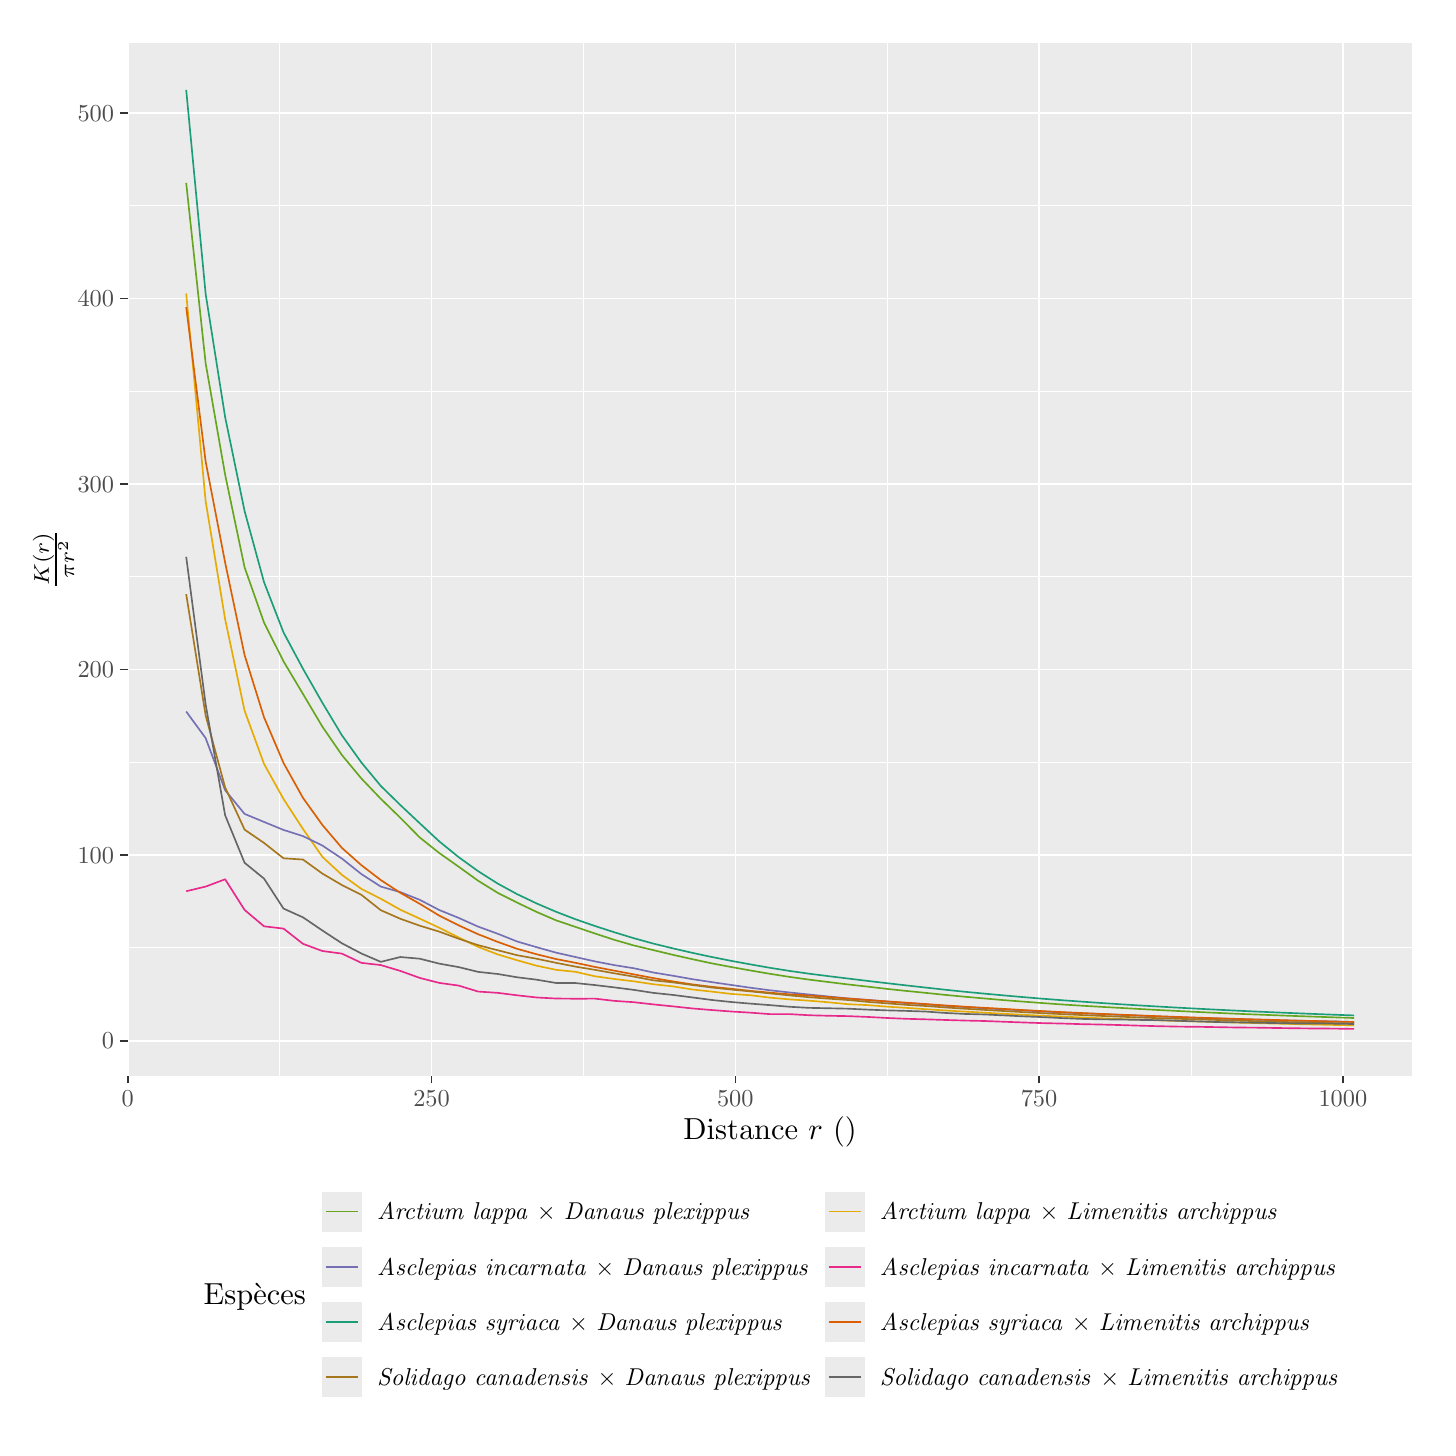
\begin{tikzpicture}[x=1pt,y=1pt]
\definecolor{fillColor}{RGB}{255,255,255}
\path[use as bounding box,fill=fillColor,fill opacity=0.00] (0,0) rectangle (505.89,505.89);
\begin{scope}
\path[clip] (  0.00,  0.00) rectangle (505.89,505.89);
\definecolor{drawColor}{RGB}{255,255,255}
\definecolor{fillColor}{RGB}{255,255,255}

\path[draw=drawColor,line width= 0.6pt,line join=round,line cap=round,fill=fillColor] (  0.00,  0.00) rectangle (505.89,505.89);
\end{scope}
\begin{scope}
\path[clip] ( 36.18,127.12) rectangle (500.39,500.39);
\definecolor{fillColor}{gray}{0.92}

\path[fill=fillColor] ( 36.18,127.12) rectangle (500.39,500.39);
\definecolor{drawColor}{RGB}{255,255,255}

\path[draw=drawColor,line width= 0.3pt,line join=round] ( 36.18,173.36) --
	(500.39,173.36);

\path[draw=drawColor,line width= 0.3pt,line join=round] ( 36.18,240.41) --
	(500.39,240.41);

\path[draw=drawColor,line width= 0.3pt,line join=round] ( 36.18,307.46) --
	(500.39,307.46);

\path[draw=drawColor,line width= 0.3pt,line join=round] ( 36.18,374.50) --
	(500.39,374.50);

\path[draw=drawColor,line width= 0.3pt,line join=round] ( 36.18,441.55) --
	(500.39,441.55);

\path[draw=drawColor,line width= 0.3pt,line join=round] ( 91.06,127.12) --
	( 91.06,500.39);

\path[draw=drawColor,line width= 0.3pt,line join=round] (200.83,127.12) --
	(200.83,500.39);

\path[draw=drawColor,line width= 0.3pt,line join=round] (310.59,127.12) --
	(310.59,500.39);

\path[draw=drawColor,line width= 0.3pt,line join=round] (420.35,127.12) --
	(420.35,500.39);

\path[draw=drawColor,line width= 0.6pt,line join=round] ( 36.18,139.84) --
	(500.39,139.84);

\path[draw=drawColor,line width= 0.6pt,line join=round] ( 36.18,206.89) --
	(500.39,206.89);

\path[draw=drawColor,line width= 0.6pt,line join=round] ( 36.18,273.93) --
	(500.39,273.93);

\path[draw=drawColor,line width= 0.6pt,line join=round] ( 36.18,340.98) --
	(500.39,340.98);

\path[draw=drawColor,line width= 0.6pt,line join=round] ( 36.18,408.03) --
	(500.39,408.03);

\path[draw=drawColor,line width= 0.6pt,line join=round] ( 36.18,475.07) --
	(500.39,475.07);

\path[draw=drawColor,line width= 0.6pt,line join=round] ( 36.18,127.12) --
	( 36.18,500.39);

\path[draw=drawColor,line width= 0.6pt,line join=round] (145.94,127.12) --
	(145.94,500.39);

\path[draw=drawColor,line width= 0.6pt,line join=round] (255.71,127.12) --
	(255.71,500.39);

\path[draw=drawColor,line width= 0.6pt,line join=round] (365.47,127.12) --
	(365.47,500.39);

\path[draw=drawColor,line width= 0.6pt,line join=round] (475.24,127.12) --
	(475.24,500.39);
\definecolor{drawColor}{RGB}{102,166,30}

\path[draw=drawColor,line width= 0.6pt,line join=round] ( 57.28,449.77) --
	( 64.31,384.61) --
	( 71.35,344.36) --
	( 78.38,310.88) --
	( 85.41,290.90) --
	( 92.45,276.91) --
	( 99.48,265.12) --
	(106.51,253.28) --
	(113.55,243.05) --
	(120.58,234.58) --
	(127.61,227.23) --
	(134.65,220.39) --
	(141.68,213.26) --
	(148.72,207.65) --
	(155.75,202.69) --
	(162.78,197.62) --
	(169.82,193.28) --
	(176.85,189.73) --
	(183.88,186.37) --
	(190.92,183.33) --
	(197.95,180.95) --
	(204.98,178.57) --
	(212.02,176.26) --
	(219.05,174.24) --
	(226.08,172.56) --
	(233.12,170.87) --
	(240.15,169.29) --
	(247.18,167.78) --
	(254.22,166.45) --
	(261.25,165.19) --
	(268.28,163.99) --
	(275.32,162.88) --
	(282.35,161.90) --
	(289.39,161.02) --
	(296.42,160.16) --
	(303.45,159.37) --
	(310.49,158.55) --
	(317.52,157.81) --
	(324.55,157.11) --
	(331.59,156.38) --
	(338.62,155.72) --
	(345.65,155.10) --
	(352.69,154.49) --
	(359.72,153.95) --
	(366.75,153.43) --
	(373.79,152.92) --
	(380.82,152.48) --
	(387.85,152.07) --
	(394.89,151.68) --
	(401.92,151.28) --
	(408.95,150.90) --
	(415.99,150.55) --
	(423.02,150.20) --
	(430.06,149.87) --
	(437.09,149.56) --
	(444.12,149.28) --
	(451.16,149.01) --
	(458.19,148.75) --
	(465.22,148.51) --
	(472.26,148.26) --
	(479.29,148.03);
\definecolor{drawColor}{RGB}{230,171,2}

\path[draw=drawColor,line width= 0.6pt,line join=round] ( 57.28,409.82) --
	( 64.31,334.73) --
	( 71.35,292.11) --
	( 78.38,259.08) --
	( 85.41,239.84) --
	( 92.45,227.16) --
	( 99.48,216.33) --
	(106.51,206.25) --
	(113.55,199.75) --
	(120.58,194.68) --
	(127.61,191.12) --
	(134.65,187.16) --
	(141.68,183.94) --
	(148.72,180.65) --
	(155.75,177.11) --
	(162.78,173.71) --
	(169.82,171.03) --
	(176.85,168.90) --
	(183.88,166.93) --
	(190.92,165.44) --
	(197.95,164.72) --
	(204.98,163.11) --
	(212.02,162.13) --
	(219.05,161.29) --
	(226.08,160.23) --
	(233.12,159.47) --
	(240.15,158.33) --
	(247.18,157.57) --
	(254.22,156.74) --
	(261.25,156.25) --
	(268.28,155.38) --
	(275.32,154.76) --
	(282.35,154.29) --
	(289.39,153.71) --
	(296.42,153.03) --
	(303.45,152.69) --
	(310.49,152.14) --
	(317.52,151.69) --
	(324.55,151.21) --
	(331.59,150.75) --
	(338.62,150.35) --
	(345.65,149.96) --
	(352.69,149.56) --
	(359.72,149.18) --
	(366.75,148.84) --
	(373.79,148.56) --
	(380.82,148.22) --
	(387.85,147.94) --
	(394.89,147.66) --
	(401.92,147.43) --
	(408.95,147.18) --
	(415.99,146.95) --
	(423.02,146.78) --
	(430.06,146.56) --
	(437.09,146.37) --
	(444.12,146.18) --
	(451.16,146.01) --
	(458.19,145.83) --
	(465.22,145.68) --
	(472.26,145.52) --
	(479.29,145.38);
\definecolor{drawColor}{RGB}{117,112,179}

\path[draw=drawColor,line width= 0.6pt,line join=round] ( 57.28,258.78) --
	( 64.31,249.17) --
	( 71.35,230.35) --
	( 78.38,221.79) --
	( 85.41,218.88) --
	( 92.45,215.99) --
	( 99.48,213.76) --
	(106.51,210.34) --
	(113.55,205.65) --
	(120.58,200.04) --
	(127.61,195.51) --
	(134.65,193.52) --
	(141.68,190.74) --
	(148.72,187.06) --
	(155.75,184.20) --
	(162.78,181.05) --
	(169.82,178.49) --
	(176.85,175.68) --
	(183.88,173.63) --
	(190.92,171.65) --
	(197.95,170.06) --
	(204.98,168.49) --
	(212.02,167.13) --
	(219.05,166.01) --
	(226.08,164.47) --
	(233.12,163.31) --
	(240.15,162.07) --
	(247.18,161.00) --
	(254.22,159.97) --
	(261.25,158.96) --
	(268.28,158.04) --
	(275.32,157.26) --
	(282.35,156.52) --
	(289.39,155.80) --
	(296.42,155.10) --
	(303.45,154.58) --
	(310.49,154.00) --
	(317.52,153.41) --
	(324.55,152.94) --
	(331.59,152.42) --
	(338.62,151.99) --
	(345.65,151.54) --
	(352.69,151.15) --
	(359.72,150.76) --
	(366.75,150.39) --
	(373.79,150.04) --
	(380.82,149.73) --
	(387.85,149.47) --
	(394.89,149.16) --
	(401.92,148.88) --
	(408.95,148.57) --
	(415.99,148.32) --
	(423.02,148.06) --
	(430.06,147.87) --
	(437.09,147.64) --
	(444.12,147.43) --
	(451.16,147.22) --
	(458.19,147.05) --
	(465.22,146.94) --
	(472.26,146.78) --
	(479.29,146.60);
\definecolor{drawColor}{RGB}{231,41,138}

\path[draw=drawColor,line width= 0.6pt,line join=round] ( 57.28,193.84) --
	( 64.31,195.52) --
	( 71.35,198.16) --
	( 78.38,187.09) --
	( 85.41,181.16) --
	( 92.45,180.34) --
	( 99.48,174.84) --
	(106.51,172.24) --
	(113.55,171.30) --
	(120.58,167.96) --
	(127.61,167.16) --
	(134.65,165.05) --
	(141.68,162.52) --
	(148.72,160.72) --
	(155.75,159.74) --
	(162.78,157.59) --
	(169.82,157.12) --
	(176.85,156.24) --
	(183.88,155.45) --
	(190.92,155.07) --
	(197.95,155.00) --
	(204.98,155.03) --
	(212.02,154.22) --
	(219.05,153.74) --
	(226.08,152.95) --
	(233.12,152.24) --
	(240.15,151.49) --
	(247.18,150.91) --
	(254.22,150.38) --
	(261.25,149.96) --
	(268.28,149.43) --
	(275.32,149.44) --
	(282.35,149.03) --
	(289.39,148.84) --
	(296.42,148.71) --
	(303.45,148.42) --
	(310.49,148.04) --
	(317.52,147.74) --
	(324.55,147.55) --
	(331.59,147.32) --
	(338.62,147.11) --
	(345.65,146.95) --
	(352.69,146.68) --
	(359.72,146.42) --
	(366.75,146.18) --
	(373.79,146.03) --
	(380.82,145.81) --
	(387.85,145.67) --
	(394.89,145.48) --
	(401.92,145.26) --
	(408.95,145.06) --
	(415.99,144.92) --
	(423.02,144.85) --
	(430.06,144.72) --
	(437.09,144.60) --
	(444.12,144.54) --
	(451.16,144.42) --
	(458.19,144.32) --
	(465.22,144.24) --
	(472.26,144.20) --
	(479.29,144.09);
\definecolor{drawColor}{RGB}{27,158,119}

\path[draw=drawColor,line width= 0.6pt,line join=round] ( 57.28,483.42) --
	( 64.31,409.69) --
	( 71.35,365.19) --
	( 78.38,331.22) --
	( 85.41,305.51) --
	( 92.45,287.35) --
	( 99.48,274.23) --
	(106.51,261.91) --
	(113.55,250.18) --
	(120.58,240.37) --
	(127.61,231.88) --
	(134.65,225.00) --
	(141.68,218.39) --
	(148.72,211.86) --
	(155.75,206.14) --
	(162.78,201.08) --
	(169.82,196.62) --
	(176.85,192.79) --
	(183.88,189.44) --
	(190.92,186.42) --
	(197.95,183.72) --
	(204.98,181.27) --
	(212.02,179.00) --
	(219.05,176.86) --
	(226.08,174.92) --
	(233.12,173.20) --
	(240.15,171.58) --
	(247.18,170.08) --
	(254.22,168.68) --
	(261.25,167.39) --
	(268.28,166.16) --
	(275.32,165.04) --
	(282.35,164.05) --
	(289.39,163.15) --
	(296.42,162.30) --
	(303.45,161.44) --
	(310.49,160.61) --
	(317.52,159.81) --
	(324.55,159.02) --
	(331.59,158.24) --
	(338.62,157.51) --
	(345.65,156.84) --
	(352.69,156.20) --
	(359.72,155.58) --
	(366.75,155.00) --
	(373.79,154.46) --
	(380.82,153.95) --
	(387.85,153.46) --
	(394.89,153.00) --
	(401.92,152.56) --
	(408.95,152.15) --
	(415.99,151.75) --
	(423.02,151.38) --
	(430.06,151.02) --
	(437.09,150.68) --
	(444.12,150.35) --
	(451.16,150.05) --
	(458.19,149.76) --
	(465.22,149.48) --
	(472.26,149.21) --
	(479.29,148.96);
\definecolor{drawColor}{RGB}{217,95,2}

\path[draw=drawColor,line width= 0.6pt,line join=round] ( 57.28,404.92) --
	( 64.31,349.10) --
	( 71.35,312.60) --
	( 78.38,279.17) --
	( 85.41,256.68) --
	( 92.45,240.19) --
	( 99.48,227.57) --
	(106.51,217.76) --
	(113.55,209.49) --
	(120.58,203.26) --
	(127.61,197.87) --
	(134.65,193.27) --
	(141.68,189.30) --
	(148.72,185.03) --
	(155.75,181.50) --
	(162.78,178.30) --
	(169.82,175.54) --
	(176.85,173.04) --
	(183.88,171.07) --
	(190.92,169.34) --
	(197.95,167.98) --
	(204.98,166.48) --
	(212.02,165.13) --
	(219.05,163.79) --
	(226.08,162.45) --
	(233.12,161.26) --
	(240.15,160.18) --
	(247.18,159.30) --
	(254.22,158.59) --
	(261.25,157.83) --
	(268.28,157.18) --
	(275.32,156.58) --
	(282.35,156.16) --
	(289.39,155.60) --
	(296.42,155.06) --
	(303.45,154.53) --
	(310.49,154.02) --
	(317.52,153.57) --
	(324.55,153.08) --
	(331.59,152.56) --
	(338.62,152.11) --
	(345.65,151.71) --
	(352.69,151.32) --
	(359.72,150.90) --
	(366.75,150.52) --
	(373.79,150.15) --
	(380.82,149.83) --
	(387.85,149.51) --
	(394.89,149.22) --
	(401.92,148.94) --
	(408.95,148.66) --
	(415.99,148.40) --
	(423.02,148.15) --
	(430.06,147.92) --
	(437.09,147.70) --
	(444.12,147.50) --
	(451.16,147.31) --
	(458.19,147.11) --
	(465.22,146.93) --
	(472.26,146.76) --
	(479.29,146.59);
\definecolor{drawColor}{RGB}{166,118,29}

\path[draw=drawColor,line width= 0.6pt,line join=round] ( 57.28,301.19) --
	( 64.31,257.33) --
	( 71.35,231.35) --
	( 78.38,216.10) --
	( 85.41,211.29) --
	( 92.45,205.74) --
	( 99.48,205.29) --
	(106.51,200.21) --
	(113.55,196.07) --
	(120.58,192.54) --
	(127.61,186.98) --
	(134.65,183.89) --
	(141.68,181.39) --
	(148.72,179.24) --
	(155.75,176.67) --
	(162.78,174.35) --
	(169.82,172.52) --
	(176.85,170.72) --
	(183.88,169.45) --
	(190.92,167.97) --
	(197.95,166.60) --
	(204.98,165.43) --
	(212.02,164.17) --
	(219.05,162.98) --
	(226.08,161.64) --
	(233.12,160.90) --
	(240.15,159.95) --
	(247.18,159.05) --
	(254.22,158.30) --
	(261.25,157.64) --
	(268.28,156.91) --
	(275.32,156.20) --
	(282.35,155.54) --
	(289.39,155.02) --
	(296.42,154.53) --
	(303.45,153.86) --
	(310.49,153.32) --
	(317.52,152.78) --
	(324.55,152.36) --
	(331.59,151.84) --
	(338.62,151.38) --
	(345.65,150.96) --
	(352.69,150.55) --
	(359.72,150.15) --
	(366.75,149.77) --
	(373.79,149.43) --
	(380.82,149.10) --
	(387.85,148.79) --
	(394.89,148.50) --
	(401.92,148.21) --
	(408.95,147.96) --
	(415.99,147.73) --
	(423.02,147.54) --
	(430.06,147.31) --
	(437.09,147.10) --
	(444.12,146.88) --
	(451.16,146.67) --
	(458.19,146.49) --
	(465.22,146.35) --
	(472.26,146.18) --
	(479.29,146.05);
\definecolor{drawColor}{gray}{0.40}

\path[draw=drawColor,line width= 0.6pt,line join=round] ( 57.28,314.68) --
	( 64.31,261.33) --
	( 71.35,221.30) --
	( 78.38,204.12) --
	( 85.41,198.40) --
	( 92.45,187.57) --
	( 99.48,184.41) --
	(106.51,179.64) --
	(113.55,175.03) --
	(120.58,171.34) --
	(127.61,168.32) --
	(134.65,170.07) --
	(141.68,169.46) --
	(148.72,167.68) --
	(155.75,166.42) --
	(162.78,164.70) --
	(169.82,163.94) --
	(176.85,162.75) --
	(183.88,161.88) --
	(190.92,160.69) --
	(197.95,160.66) --
	(204.98,159.93) --
	(212.02,159.09) --
	(219.05,158.19) --
	(226.08,157.11) --
	(233.12,156.37) --
	(240.15,155.47) --
	(247.18,154.55) --
	(254.22,153.81) --
	(261.25,153.22) --
	(268.28,152.68) --
	(275.32,152.09) --
	(282.35,151.70) --
	(289.39,151.55) --
	(296.42,151.40) --
	(303.45,151.06) --
	(310.49,150.79) --
	(317.52,150.60) --
	(324.55,150.36) --
	(331.59,149.86) --
	(338.62,149.50) --
	(345.65,149.31) --
	(352.69,148.98) --
	(359.72,148.63) --
	(366.75,148.35) --
	(373.79,148.00) --
	(380.82,147.71) --
	(387.85,147.54) --
	(394.89,147.49) --
	(401.92,147.34) --
	(408.95,147.25) --
	(415.99,147.01) --
	(423.02,146.79) --
	(430.06,146.57) --
	(437.09,146.45) --
	(444.12,146.31) --
	(451.16,146.20) --
	(458.19,146.06) --
	(465.22,146.06) --
	(472.26,145.98) --
	(479.29,145.86);
\end{scope}
\begin{scope}
\path[clip] (  0.00,  0.00) rectangle (505.89,505.89);
\definecolor{drawColor}{gray}{0.30}

\node[text=drawColor,anchor=base east,inner sep=0pt, outer sep=0pt, scale=  0.88] at ( 31.23,136.84) {0};

\node[text=drawColor,anchor=base east,inner sep=0pt, outer sep=0pt, scale=  0.88] at ( 31.23,203.88) {100};

\node[text=drawColor,anchor=base east,inner sep=0pt, outer sep=0pt, scale=  0.88] at ( 31.23,270.93) {200};

\node[text=drawColor,anchor=base east,inner sep=0pt, outer sep=0pt, scale=  0.88] at ( 31.23,337.97) {300};

\node[text=drawColor,anchor=base east,inner sep=0pt, outer sep=0pt, scale=  0.88] at ( 31.23,405.02) {400};

\node[text=drawColor,anchor=base east,inner sep=0pt, outer sep=0pt, scale=  0.88] at ( 31.23,472.07) {500};
\end{scope}
\begin{scope}
\path[clip] (  0.00,  0.00) rectangle (505.89,505.89);
\definecolor{drawColor}{gray}{0.20}

\path[draw=drawColor,line width= 0.6pt,line join=round] ( 33.43,139.84) --
	( 36.18,139.84);

\path[draw=drawColor,line width= 0.6pt,line join=round] ( 33.43,206.89) --
	( 36.18,206.89);

\path[draw=drawColor,line width= 0.6pt,line join=round] ( 33.43,273.93) --
	( 36.18,273.93);

\path[draw=drawColor,line width= 0.6pt,line join=round] ( 33.43,340.98) --
	( 36.18,340.98);

\path[draw=drawColor,line width= 0.6pt,line join=round] ( 33.43,408.03) --
	( 36.18,408.03);

\path[draw=drawColor,line width= 0.6pt,line join=round] ( 33.43,475.07) --
	( 36.18,475.07);
\end{scope}
\begin{scope}
\path[clip] (  0.00,  0.00) rectangle (505.89,505.89);
\definecolor{drawColor}{gray}{0.20}

\path[draw=drawColor,line width= 0.6pt,line join=round] ( 36.18,124.37) --
	( 36.18,127.12);

\path[draw=drawColor,line width= 0.6pt,line join=round] (145.94,124.37) --
	(145.94,127.12);

\path[draw=drawColor,line width= 0.6pt,line join=round] (255.71,124.37) --
	(255.71,127.12);

\path[draw=drawColor,line width= 0.6pt,line join=round] (365.47,124.37) --
	(365.47,127.12);

\path[draw=drawColor,line width= 0.6pt,line join=round] (475.24,124.37) --
	(475.24,127.12);
\end{scope}
\begin{scope}
\path[clip] (  0.00,  0.00) rectangle (505.89,505.89);
\definecolor{drawColor}{gray}{0.30}

\node[text=drawColor,anchor=base,inner sep=0pt, outer sep=0pt, scale=  0.88] at ( 36.18,116.16) {0};

\node[text=drawColor,anchor=base,inner sep=0pt, outer sep=0pt, scale=  0.88] at (145.94,116.16) {250};

\node[text=drawColor,anchor=base,inner sep=0pt, outer sep=0pt, scale=  0.88] at (255.71,116.16) {500};

\node[text=drawColor,anchor=base,inner sep=0pt, outer sep=0pt, scale=  0.88] at (365.47,116.16) {750};

\node[text=drawColor,anchor=base,inner sep=0pt, outer sep=0pt, scale=  0.88] at (475.24,116.16) {1000};
\end{scope}
\begin{scope}
\path[clip] (  0.00,  0.00) rectangle (505.89,505.89);
\definecolor{drawColor}{RGB}{0,0,0}

\node[text=drawColor,anchor=base,inner sep=0pt, outer sep=0pt, scale=  1.10] at (268.28,104.08) {Distance $r$ (\unit{\m})};
\end{scope}
\begin{scope}
\path[clip] (  0.00,  0.00) rectangle (505.89,505.89);
\definecolor{drawColor}{RGB}{0,0,0}

\node[text=drawColor,rotate= 90.00,anchor=base,inner sep=0pt, outer sep=0pt, scale=  1.10] at ( 13.01,313.75) {$\frac{K(r)}{\pi r^2}$};
\end{scope}
\begin{scope}
\path[clip] (  0.00,  0.00) rectangle (505.89,505.89);
\definecolor{fillColor}{RGB}{255,255,255}

\path[fill=fillColor] ( 58.08,  5.50) rectangle (478.49, 90.82);
\end{scope}
\begin{scope}
\path[clip] (  0.00,  0.00) rectangle (505.89,505.89);
\definecolor{drawColor}{RGB}{0,0,0}

\node[text=drawColor,anchor=base west,inner sep=0pt, outer sep=0pt, scale=  1.10] at ( 63.58, 44.40) {Espèces};
\end{scope}
\begin{scope}
\path[clip] (  0.00,  0.00) rectangle (505.89,505.89);
\definecolor{fillColor}{gray}{0.92}

\path[fill=fillColor] (106.31, 70.86) rectangle (120.77, 85.32);
\definecolor{drawColor}{RGB}{102,166,30}

\path[draw=drawColor,line width= 0.6pt,line join=round] (107.76, 78.09) -- (119.32, 78.09);
\end{scope}
\begin{scope}
\path[clip] (  0.00,  0.00) rectangle (505.89,505.89);
\definecolor{fillColor}{gray}{0.92}

\path[fill=fillColor] (287.98, 70.86) rectangle (302.43, 85.32);
\definecolor{drawColor}{RGB}{230,171,2}

\path[draw=drawColor,line width= 0.6pt,line join=round] (289.42, 78.09) -- (300.98, 78.09);
\end{scope}
\begin{scope}
\path[clip] (  0.00,  0.00) rectangle (505.89,505.89);
\definecolor{fillColor}{gray}{0.92}

\path[fill=fillColor] (106.31, 50.91) rectangle (120.77, 65.36);
\definecolor{drawColor}{RGB}{117,112,179}

\path[draw=drawColor,line width= 0.6pt,line join=round] (107.76, 58.14) -- (119.32, 58.14);
\end{scope}
\begin{scope}
\path[clip] (  0.00,  0.00) rectangle (505.89,505.89);
\definecolor{fillColor}{gray}{0.92}

\path[fill=fillColor] (287.98, 50.91) rectangle (302.43, 65.36);
\definecolor{drawColor}{RGB}{231,41,138}

\path[draw=drawColor,line width= 0.6pt,line join=round] (289.42, 58.14) -- (300.98, 58.14);
\end{scope}
\begin{scope}
\path[clip] (  0.00,  0.00) rectangle (505.89,505.89);
\definecolor{fillColor}{gray}{0.92}

\path[fill=fillColor] (106.31, 30.95) rectangle (120.77, 45.41);
\definecolor{drawColor}{RGB}{27,158,119}

\path[draw=drawColor,line width= 0.6pt,line join=round] (107.76, 38.18) -- (119.32, 38.18);
\end{scope}
\begin{scope}
\path[clip] (  0.00,  0.00) rectangle (505.89,505.89);
\definecolor{fillColor}{gray}{0.92}

\path[fill=fillColor] (287.98, 30.95) rectangle (302.43, 45.41);
\definecolor{drawColor}{RGB}{217,95,2}

\path[draw=drawColor,line width= 0.6pt,line join=round] (289.42, 38.18) -- (300.98, 38.18);
\end{scope}
\begin{scope}
\path[clip] (  0.00,  0.00) rectangle (505.89,505.89);
\definecolor{fillColor}{gray}{0.92}

\path[fill=fillColor] (106.31, 11.00) rectangle (120.77, 25.45);
\definecolor{drawColor}{RGB}{166,118,29}

\path[draw=drawColor,line width= 0.6pt,line join=round] (107.76, 18.23) -- (119.32, 18.23);
\end{scope}
\begin{scope}
\path[clip] (  0.00,  0.00) rectangle (505.89,505.89);
\definecolor{fillColor}{gray}{0.92}

\path[fill=fillColor] (287.98, 11.00) rectangle (302.43, 25.45);
\definecolor{drawColor}{gray}{0.40}

\path[draw=drawColor,line width= 0.6pt,line join=round] (289.42, 18.23) -- (300.98, 18.23);
\end{scope}
\begin{scope}
\path[clip] (  0.00,  0.00) rectangle (505.89,505.89);
\definecolor{drawColor}{RGB}{0,0,0}

\node[text=drawColor,anchor=base west,inner sep=0pt, outer sep=0pt, scale=  0.88] at (126.27, 75.08) {\textit{Arctium lappa} $\times$ \textit{Danaus plexippus}};
\end{scope}
\begin{scope}
\path[clip] (  0.00,  0.00) rectangle (505.89,505.89);
\definecolor{drawColor}{RGB}{0,0,0}

\node[text=drawColor,anchor=base west,inner sep=0pt, outer sep=0pt, scale=  0.88] at (307.93, 75.08) {\textit{Arctium lappa} $\times$ \textit{Limenitis archippus}};
\end{scope}
\begin{scope}
\path[clip] (  0.00,  0.00) rectangle (505.89,505.89);
\definecolor{drawColor}{RGB}{0,0,0}

\node[text=drawColor,anchor=base west,inner sep=0pt, outer sep=0pt, scale=  0.88] at (126.27, 55.13) {\textit{Asclepias incarnata} $\times$ \textit{Danaus plexippus}};
\end{scope}
\begin{scope}
\path[clip] (  0.00,  0.00) rectangle (505.89,505.89);
\definecolor{drawColor}{RGB}{0,0,0}

\node[text=drawColor,anchor=base west,inner sep=0pt, outer sep=0pt, scale=  0.88] at (307.93, 55.13) {\textit{Asclepias incarnata} $\times$ \textit{Limenitis archippus}};
\end{scope}
\begin{scope}
\path[clip] (  0.00,  0.00) rectangle (505.89,505.89);
\definecolor{drawColor}{RGB}{0,0,0}

\node[text=drawColor,anchor=base west,inner sep=0pt, outer sep=0pt, scale=  0.88] at (126.27, 35.18) {\textit{Asclepias syriaca} $\times$ \textit{Danaus plexippus}};
\end{scope}
\begin{scope}
\path[clip] (  0.00,  0.00) rectangle (505.89,505.89);
\definecolor{drawColor}{RGB}{0,0,0}

\node[text=drawColor,anchor=base west,inner sep=0pt, outer sep=0pt, scale=  0.88] at (307.93, 35.18) {\textit{Asclepias syriaca} $\times$ \textit{Limenitis archippus}};
\end{scope}
\begin{scope}
\path[clip] (  0.00,  0.00) rectangle (505.89,505.89);
\definecolor{drawColor}{RGB}{0,0,0}

\node[text=drawColor,anchor=base west,inner sep=0pt, outer sep=0pt, scale=  0.88] at (126.27, 15.22) {\textit{Solidago canadensis} $\times$ \textit{Danaus plexippus}};
\end{scope}
\begin{scope}
\path[clip] (  0.00,  0.00) rectangle (505.89,505.89);
\definecolor{drawColor}{RGB}{0,0,0}

\node[text=drawColor,anchor=base west,inner sep=0pt, outer sep=0pt, scale=  0.88] at (307.93, 15.22) {\textit{Solidago canadensis} $\times$ \textit{Limenitis archippus}};
\end{scope}
\end{tikzpicture}
%
        }
    \end{figure}
    \begin{figure}[H]
        \centering
        \caption{Corrélation normalisée entre les espèces pour $r \ge \SI{1}{\km}$}
        \resize{%
            % Created by tikzDevice version 0.12.6 on 2025-11-09 21:39:43
% !TEX encoding = UTF-8 Unicode
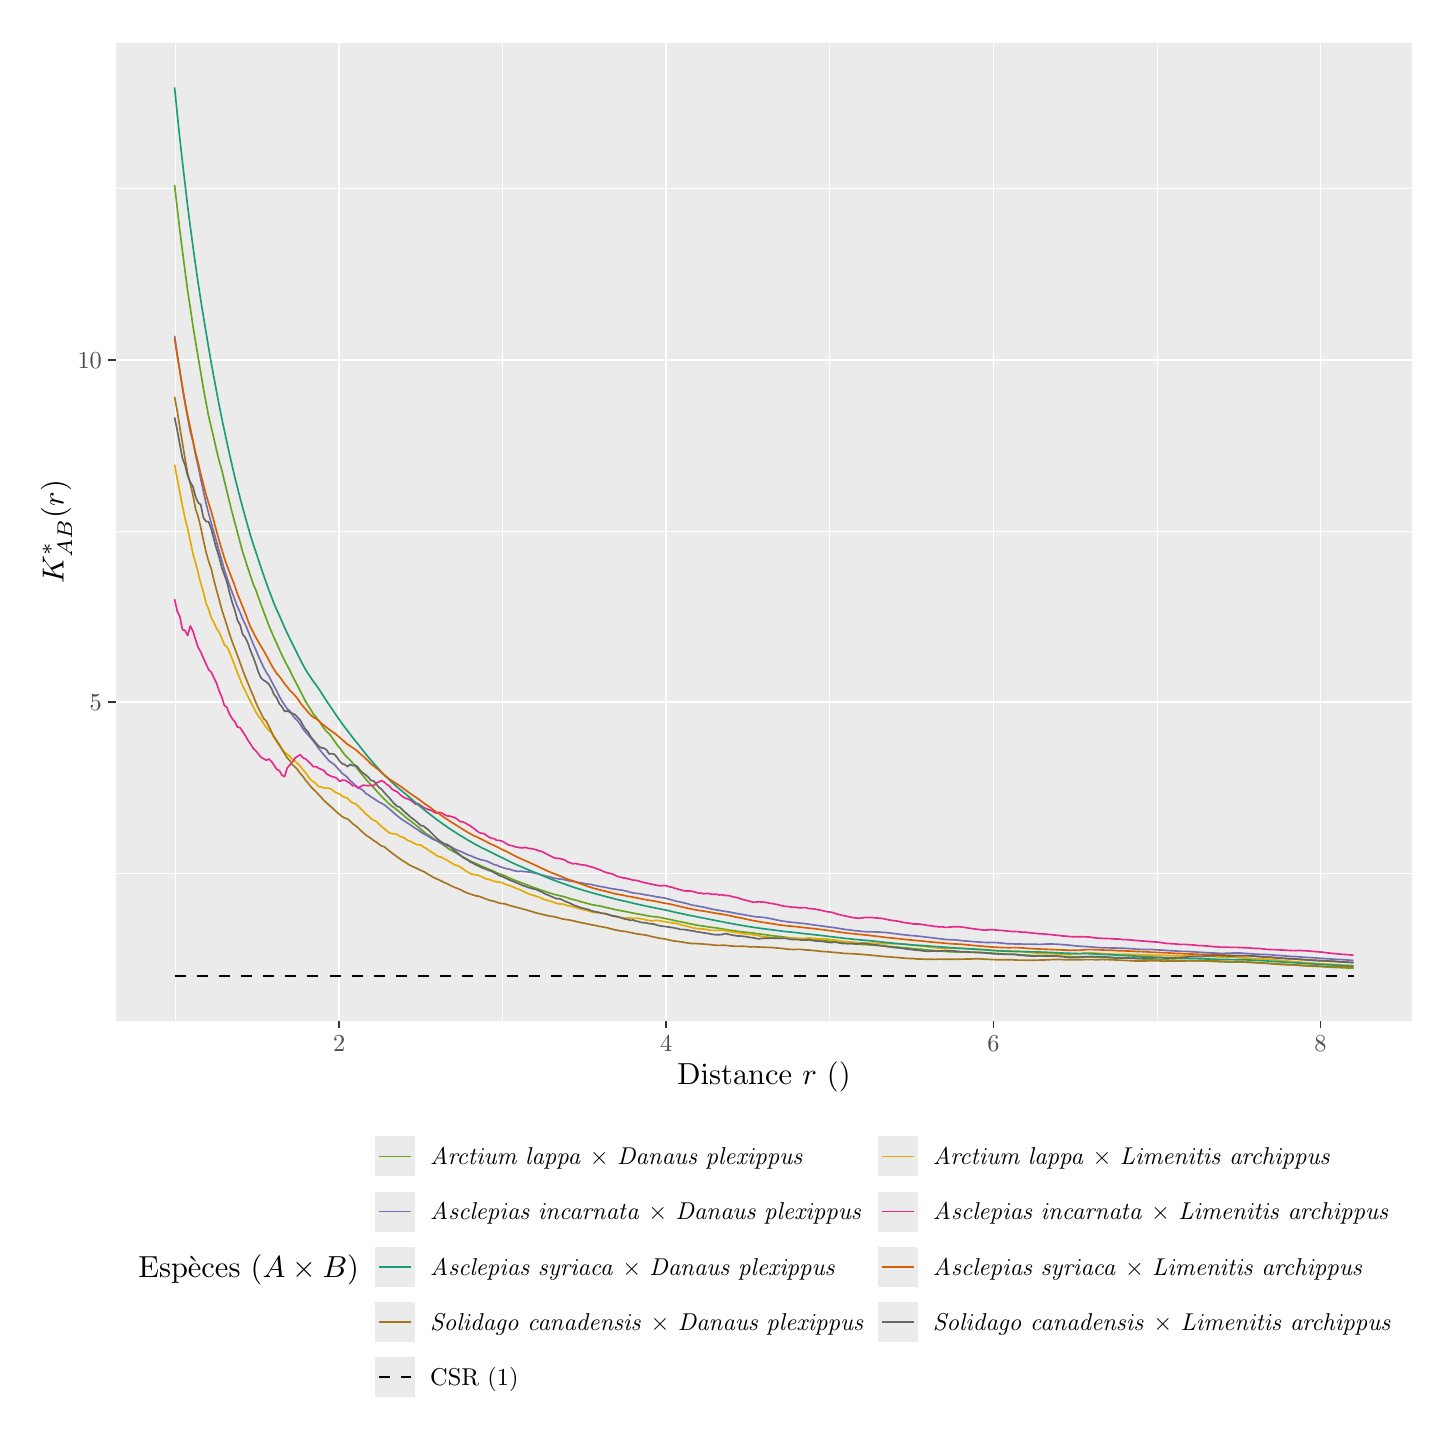
\begin{tikzpicture}[x=1pt,y=1pt]
\definecolor{fillColor}{RGB}{255,255,255}
\path[use as bounding box,fill=fillColor,fill opacity=0.00] (0,0) rectangle (505.89,505.89);
\begin{scope}
\path[clip] (  0.00,  0.00) rectangle (505.89,505.89);
\definecolor{drawColor}{RGB}{255,255,255}
\definecolor{fillColor}{RGB}{255,255,255}

\path[draw=drawColor,line width= 0.6pt,line join=round,line cap=round,fill=fillColor] (  0.00,  0.00) rectangle (505.89,505.89);
\end{scope}
\begin{scope}
\path[clip] ( 31.78,147.07) rectangle (500.39,500.39);
\definecolor{fillColor}{gray}{0.92}

\path[fill=fillColor] ( 31.78,147.07) rectangle (500.39,500.39);
\definecolor{drawColor}{RGB}{255,255,255}

\path[draw=drawColor,line width= 0.3pt,line join=round] ( 31.78,200.26) --
	(500.39,200.26);

\path[draw=drawColor,line width= 0.3pt,line join=round] ( 31.78,324.03) --
	(500.39,324.03);

\path[draw=drawColor,line width= 0.3pt,line join=round] ( 31.78,447.79) --
	(500.39,447.79);

\path[draw=drawColor,line width= 0.3pt,line join=round] ( 53.48,147.07) --
	( 53.48,500.39);

\path[draw=drawColor,line width= 0.3pt,line join=round] (171.67,147.07) --
	(171.67,500.39);

\path[draw=drawColor,line width= 0.3pt,line join=round] (289.86,147.07) --
	(289.86,500.39);

\path[draw=drawColor,line width= 0.3pt,line join=round] (408.06,147.07) --
	(408.06,500.39);

\path[draw=drawColor,line width= 0.6pt,line join=round] ( 31.78,262.14) --
	(500.39,262.14);

\path[draw=drawColor,line width= 0.6pt,line join=round] ( 31.78,385.91) --
	(500.39,385.91);

\path[draw=drawColor,line width= 0.6pt,line join=round] (112.58,147.07) --
	(112.58,500.39);

\path[draw=drawColor,line width= 0.6pt,line join=round] (230.77,147.07) --
	(230.77,500.39);

\path[draw=drawColor,line width= 0.6pt,line join=round] (348.96,147.07) --
	(348.96,500.39);

\path[draw=drawColor,line width= 0.6pt,line join=round] (467.15,147.07) --
	(467.15,500.39);
\definecolor{drawColor}{RGB}{0,0,0}

\path[draw=drawColor,line width= 0.6pt,dash pattern=on 4pt off 4pt ,line join=round] ( 53.08,163.13) --
	(479.09,163.13);
\definecolor{drawColor}{RGB}{102,166,30}

\path[draw=drawColor,line width= 0.6pt,line join=round] ( 53.08,449.05) --
	( 54.03,440.79) --
	( 54.97,432.71) --
	( 55.92,425.23) --
	( 56.87,417.94) --
	( 57.81,410.74) --
	( 58.76,404.66) --
	( 59.71,398.16) --
	( 60.65,392.51) --
	( 61.60,386.78) --
	( 62.55,381.25) --
	( 63.49,375.52) --
	( 64.44,370.49) --
	( 65.39,365.44) --
	( 66.33,361.55) --
	( 67.28,357.47) --
	( 68.23,353.24) --
	( 69.17,349.45) --
	( 70.12,346.18) --
	( 71.07,342.16) --
	( 72.01,338.26) --
	( 72.96,334.36) --
	( 73.91,330.59) --
	( 74.85,327.02) --
	( 75.80,323.55) --
	( 76.75,319.89) --
	( 77.69,316.44) --
	( 78.64,313.52) --
	( 79.59,310.50) --
	( 80.53,307.66) --
	( 81.48,304.85) --
	( 82.43,302.76) --
	( 83.37,300.05) --
	( 84.32,297.44) --
	( 85.27,294.88) --
	( 86.21,292.41) --
	( 87.16,289.82) --
	( 88.11,287.61) --
	( 89.05,285.42) --
	( 90.00,283.36) --
	( 90.95,281.18) --
	( 91.89,279.14) --
	( 92.84,277.23) --
	( 93.79,275.38) --
	( 94.73,273.66) --
	( 95.68,271.62) --
	( 96.63,269.80) --
	( 97.57,268.02) --
	( 98.52,266.16) --
	( 99.47,264.30) --
	(100.41,262.48) --
	(101.36,260.93) --
	(102.31,259.43) --
	(103.25,257.86) --
	(104.20,256.73) --
	(105.15,255.54) --
	(106.09,254.16) --
	(107.04,252.70) --
	(107.99,251.64) --
	(108.93,250.74) --
	(109.88,249.53) --
	(110.83,248.11) --
	(111.77,246.85) --
	(112.72,245.61) --
	(113.67,244.36) --
	(114.61,243.10) --
	(115.56,242.13) --
	(116.51,241.24) --
	(117.45,240.11) --
	(118.40,239.04) --
	(119.35,237.80) --
	(120.29,236.67) --
	(121.24,235.51) --
	(122.19,234.34) --
	(123.13,233.23) --
	(124.08,232.26) --
	(125.03,231.24) --
	(125.97,230.23) --
	(126.92,229.13) --
	(127.87,228.16) --
	(128.81,227.17) --
	(129.76,226.27) --
	(130.71,225.34) --
	(131.65,224.56) --
	(132.60,223.95) --
	(133.55,223.15) --
	(134.49,222.38) --
	(135.44,221.62) --
	(136.39,220.75) --
	(137.33,219.97) --
	(138.28,219.27) --
	(139.23,218.54) --
	(140.17,217.80) --
	(141.12,217.07) --
	(142.07,216.28) --
	(143.01,215.44) --
	(143.96,214.66) --
	(144.91,214.07) --
	(145.86,213.40) --
	(146.80,212.74) --
	(147.75,212.10) --
	(148.70,211.48) --
	(149.64,210.93) --
	(150.59,210.29) --
	(151.54,209.59) --
	(152.48,208.96) --
	(153.43,208.43) --
	(154.38,207.90) --
	(155.32,207.36) --
	(156.27,206.83) --
	(157.22,206.30) --
	(158.16,205.77) --
	(159.11,205.17) --
	(160.06,204.68) --
	(161.00,204.27) --
	(161.95,203.91) --
	(162.90,203.44) --
	(163.84,203.02) --
	(164.79,202.59) --
	(165.74,202.17) --
	(166.68,201.77) --
	(167.63,201.43) --
	(168.58,200.97) --
	(169.52,200.48) --
	(170.47,200.12) --
	(171.42,199.81) --
	(172.36,199.44) --
	(173.31,198.99) --
	(174.26,198.55) --
	(175.20,198.12) --
	(176.15,197.74) --
	(177.10,197.39) --
	(178.04,197.02) --
	(178.99,196.67) --
	(179.94,196.32) --
	(180.88,195.98) --
	(181.83,195.57) --
	(182.78,195.22) --
	(183.72,194.90) --
	(184.67,194.53) --
	(185.62,194.22) --
	(186.56,193.92) --
	(187.51,193.58) --
	(188.46,193.28) --
	(189.40,192.96) --
	(190.35,192.67) --
	(191.30,192.46) --
	(192.24,192.24) --
	(193.19,192.01) --
	(194.14,191.80) --
	(195.08,191.45) --
	(196.03,191.15) --
	(196.98,190.88) --
	(197.92,190.63) --
	(198.87,190.39) --
	(199.82,190.07) --
	(200.76,189.84) --
	(201.71,189.54) --
	(202.66,189.33) --
	(203.60,189.06) --
	(204.55,188.85) --
	(205.50,188.71) --
	(206.44,188.55) --
	(207.39,188.38) --
	(208.34,188.10) --
	(209.28,187.93) --
	(210.23,187.71) --
	(211.18,187.48) --
	(212.12,187.23) --
	(213.07,187.08) --
	(214.02,186.86) --
	(214.96,186.69) --
	(215.91,186.52) --
	(216.86,186.33) --
	(217.80,186.14) --
	(218.75,185.93) --
	(219.70,185.75) --
	(220.64,185.60) --
	(221.59,185.44) --
	(222.54,185.26) --
	(223.48,185.07) --
	(224.43,184.89) --
	(225.38,184.76) --
	(226.32,184.61) --
	(227.27,184.59) --
	(228.22,184.41) --
	(229.16,184.24) --
	(230.11,184.04) --
	(231.06,183.83) --
	(232.00,183.66) --
	(232.95,183.45) --
	(233.90,183.21) --
	(234.84,182.99) --
	(235.79,182.83) --
	(236.74,182.65) --
	(237.68,182.45) --
	(238.63,182.23) --
	(239.58,182.03) --
	(240.52,181.84) --
	(241.47,181.66) --
	(242.42,181.46) --
	(243.36,181.35) --
	(244.31,181.22) --
	(245.26,181.09) --
	(246.20,180.91) --
	(247.15,180.79) --
	(248.10,180.68) --
	(249.04,180.54) --
	(249.99,180.39) --
	(250.94,180.20) --
	(251.88,180.08) --
	(252.83,179.92) --
	(253.78,179.73) --
	(254.72,179.64) --
	(255.67,179.49) --
	(256.62,179.32) --
	(257.56,179.21) --
	(258.51,179.11) --
	(259.46,179.02) --
	(260.40,178.92) --
	(261.35,178.83) --
	(262.30,178.69) --
	(263.24,178.55) --
	(264.19,178.44) --
	(265.14,178.32) --
	(266.08,178.18) --
	(267.03,178.07) --
	(267.98,177.92) --
	(268.92,177.80) --
	(269.87,177.66) --
	(270.82,177.58) --
	(271.76,177.49) --
	(272.71,177.35) --
	(273.66,177.23) --
	(274.60,177.10) --
	(275.55,177.00) --
	(276.50,176.89) --
	(277.44,176.81) --
	(278.39,176.73) --
	(279.34,176.65) --
	(280.28,176.54) --
	(281.23,176.48) --
	(282.18,176.49) --
	(283.12,176.41) --
	(284.07,176.38) --
	(285.02,176.31) --
	(285.96,176.20) --
	(286.91,176.11) --
	(287.86,176.00) --
	(288.81,175.90) --
	(289.75,175.77) --
	(290.70,175.67) --
	(291.65,175.55) --
	(292.59,175.48) --
	(293.54,175.34) --
	(294.49,175.24) --
	(295.43,175.11) --
	(296.38,175.05) --
	(297.33,174.94) --
	(298.27,174.86) --
	(299.22,174.75) --
	(300.17,174.66) --
	(301.11,174.64) --
	(302.06,174.58) --
	(303.01,174.53) --
	(303.95,174.46) --
	(304.90,174.40) --
	(305.85,174.32) --
	(306.79,174.28) --
	(307.74,174.20) --
	(308.69,174.09) --
	(309.63,174.00) --
	(310.58,173.93) --
	(311.53,173.89) --
	(312.47,173.80) --
	(313.42,173.72) --
	(314.37,173.66) --
	(315.31,173.55) --
	(316.26,173.47) --
	(317.21,173.40) --
	(318.15,173.29) --
	(319.10,173.20) --
	(320.05,173.06) --
	(320.99,172.98) --
	(321.94,172.92) --
	(322.89,172.86) --
	(323.83,172.74) --
	(324.78,172.65) --
	(325.73,172.56) --
	(326.67,172.48) --
	(327.62,172.39) --
	(328.57,172.31) --
	(329.51,172.22) --
	(330.46,172.17) --
	(331.41,172.10) --
	(332.35,172.02) --
	(333.30,171.95) --
	(334.25,171.92) --
	(335.19,171.88) --
	(336.14,171.88) --
	(337.09,171.89) --
	(338.03,171.85) --
	(338.98,171.82) --
	(339.93,171.80) --
	(340.87,171.77) --
	(341.82,171.74) --
	(342.77,171.70) --
	(343.71,171.70) --
	(344.66,171.69) --
	(345.61,171.64) --
	(346.55,171.58) --
	(347.50,171.56) --
	(348.45,171.49) --
	(349.39,171.43) --
	(350.34,171.35) --
	(351.29,171.29) --
	(352.23,171.24) --
	(353.18,171.16) --
	(354.13,171.10) --
	(355.07,171.06) --
	(356.02,171.03) --
	(356.97,171.02) --
	(357.91,170.94) --
	(358.86,170.88) --
	(359.81,170.82) --
	(360.75,170.76) --
	(361.70,170.69) --
	(362.65,170.65) --
	(363.59,170.59) --
	(364.54,170.54) --
	(365.49,170.53) --
	(366.43,170.49) --
	(367.38,170.49) --
	(368.33,170.50) --
	(369.27,170.52) --
	(370.22,170.48) --
	(371.17,170.47) --
	(372.11,170.42) --
	(373.06,170.36) --
	(374.01,170.29) --
	(374.95,170.28) --
	(375.90,170.27) --
	(376.85,170.24) --
	(377.79,170.20) --
	(378.74,170.16) --
	(379.69,170.14) --
	(380.63,170.14) --
	(381.58,170.17) --
	(382.53,170.17) --
	(383.47,170.13) --
	(384.42,170.08) --
	(385.37,170.04) --
	(386.31,170.00) --
	(387.26,169.96) --
	(388.21,169.89) --
	(389.15,169.86) --
	(390.10,169.84) --
	(391.05,169.82) --
	(391.99,169.77) --
	(392.94,169.72) --
	(393.89,169.69) --
	(394.83,169.68) --
	(395.78,169.68) --
	(396.73,169.64) --
	(397.67,169.63) --
	(398.62,169.60) --
	(399.57,169.56) --
	(400.51,169.51) --
	(401.46,169.45) --
	(402.41,169.40) --
	(403.35,169.34) --
	(404.30,169.27) --
	(405.25,169.23) --
	(406.19,169.20) --
	(407.14,169.16) --
	(408.09,169.14) --
	(409.03,169.13) --
	(409.98,169.08) --
	(410.93,169.06) --
	(411.87,168.99) --
	(412.82,168.94) --
	(413.77,168.91) --
	(414.71,168.88) --
	(415.66,168.86) --
	(416.61,168.84) --
	(417.55,168.83) --
	(418.50,168.81) --
	(419.45,168.79) --
	(420.39,168.78) --
	(421.34,168.76) --
	(422.29,168.73) --
	(423.23,168.74) --
	(424.18,168.72) --
	(425.13,168.65) --
	(426.07,168.59) --
	(427.02,168.55) --
	(427.97,168.50) --
	(428.91,168.46) --
	(429.86,168.41) --
	(430.81,168.36) --
	(431.76,168.32) --
	(432.70,168.29) --
	(433.65,168.25) --
	(434.60,168.24) --
	(435.54,168.24) --
	(436.49,168.23) --
	(437.44,168.25) --
	(438.38,168.24) --
	(439.33,168.22) --
	(440.28,168.21) --
	(441.22,168.17) --
	(442.17,168.16) --
	(443.12,168.10) --
	(444.06,168.02) --
	(445.01,167.98) --
	(445.96,167.94) --
	(446.90,167.88) --
	(447.85,167.81) --
	(448.80,167.77) --
	(449.74,167.71) --
	(450.69,167.66) --
	(451.64,167.60) --
	(452.58,167.53) --
	(453.53,167.47) --
	(454.48,167.40) --
	(455.42,167.33) --
	(456.37,167.27) --
	(457.32,167.19) --
	(458.26,167.13) --
	(459.21,167.07) --
	(460.16,167.01) --
	(461.10,166.93) --
	(462.05,166.87) --
	(463.00,166.80) --
	(463.94,166.76) --
	(464.89,166.72) --
	(465.84,166.67) --
	(466.78,166.63) --
	(467.73,166.57) --
	(468.68,166.50) --
	(469.62,166.44) --
	(470.57,166.40) --
	(471.52,166.34) --
	(472.46,166.30) --
	(473.41,166.27) --
	(474.36,166.22) --
	(475.30,166.16) --
	(476.25,166.14) --
	(477.20,166.09) --
	(478.14,166.03) --
	(479.09,165.99);
\definecolor{drawColor}{RGB}{230,171,2}

\path[draw=drawColor,line width= 0.6pt,line join=round] ( 53.08,348.02) --
	( 54.03,342.92) --
	( 54.97,338.04) --
	( 55.92,333.01) --
	( 56.87,328.53) --
	( 57.81,324.89) --
	( 58.76,320.42) --
	( 59.71,315.81) --
	( 60.65,312.60) --
	( 61.60,308.92) --
	( 62.55,305.08) --
	( 63.49,302.00) --
	( 64.44,297.88) --
	( 65.39,295.78) --
	( 66.33,292.70) --
	( 67.28,290.99) --
	( 68.23,288.82) --
	( 69.17,287.43) --
	( 70.12,285.36) --
	( 71.07,282.90) --
	( 72.01,282.12) --
	( 72.96,280.20) --
	( 73.91,277.75) --
	( 74.85,275.32) --
	( 75.80,272.76) --
	( 76.75,270.48) --
	( 77.69,268.07) --
	( 78.64,266.12) --
	( 79.59,264.22) --
	( 80.53,262.37) --
	( 81.48,260.57) --
	( 82.43,258.65) --
	( 83.37,257.12) --
	( 84.32,255.96) --
	( 85.27,254.33) --
	( 86.21,253.07) --
	( 87.16,251.98) --
	( 88.11,251.07) --
	( 89.05,249.28) --
	( 90.00,247.83) --
	( 90.95,246.41) --
	( 91.89,245.31) --
	( 92.84,243.95) --
	( 93.79,243.44) --
	( 94.73,242.54) --
	( 95.68,241.51) --
	( 96.63,240.90) --
	( 97.57,239.91) --
	( 98.52,239.06) --
	( 99.47,237.74) --
	(100.41,236.70) --
	(101.36,235.32) --
	(102.31,234.09) --
	(103.25,233.45) --
	(104.20,232.64) --
	(105.15,231.59) --
	(106.09,231.53) --
	(107.04,231.19) --
	(107.99,231.08) --
	(108.93,231.02) --
	(109.88,230.64) --
	(110.83,229.78) --
	(111.77,229.35) --
	(112.72,228.92) --
	(113.67,228.17) --
	(114.61,227.76) --
	(115.56,227.47) --
	(116.51,226.45) --
	(117.45,225.77) --
	(118.40,225.49) --
	(119.35,224.62) --
	(120.29,223.75) --
	(121.24,222.73) --
	(122.19,221.73) --
	(123.13,221.01) --
	(124.08,220.13) --
	(125.03,219.50) --
	(125.97,219.10) --
	(126.92,218.12) --
	(127.87,217.16) --
	(128.81,216.55) --
	(129.76,215.68) --
	(130.71,214.90) --
	(131.65,214.69) --
	(132.60,214.53) --
	(133.55,214.38) --
	(134.49,213.63) --
	(135.44,213.39) --
	(136.39,212.92) --
	(137.33,212.22) --
	(138.28,211.88) --
	(139.23,211.39) --
	(140.17,210.88) --
	(141.12,210.59) --
	(142.07,210.52) --
	(143.01,209.78) --
	(143.96,209.39) --
	(144.91,208.64) --
	(145.86,208.04) --
	(146.80,207.49) --
	(147.75,206.76) --
	(148.70,206.28) --
	(149.64,206.12) --
	(150.59,205.44) --
	(151.54,205.10) --
	(152.48,204.41) --
	(153.43,203.91) --
	(154.38,203.31) --
	(155.32,203.12) --
	(156.27,202.62) --
	(157.22,201.97) --
	(158.16,201.29) --
	(159.11,200.72) --
	(160.06,200.15) --
	(161.00,199.91) --
	(161.95,199.81) --
	(162.90,199.59) --
	(163.84,199.19) --
	(164.79,198.65) --
	(165.74,198.31) --
	(166.68,198.13) --
	(167.63,197.81) --
	(168.58,197.41) --
	(169.52,197.25) --
	(170.47,197.10) --
	(171.42,196.92) --
	(172.36,196.47) --
	(173.31,196.11) --
	(174.26,195.83) --
	(175.20,195.48) --
	(176.15,195.01) --
	(177.10,194.69) --
	(178.04,194.31) --
	(178.99,193.86) --
	(179.94,193.41) --
	(180.88,193.00) --
	(181.83,192.61) --
	(182.78,192.37) --
	(183.72,192.04) --
	(184.67,191.72) --
	(185.62,191.34) --
	(186.56,190.86) --
	(187.51,190.60) --
	(188.46,190.40) --
	(189.40,190.05) --
	(190.35,189.72) --
	(191.30,189.39) --
	(192.24,189.25) --
	(193.19,189.20) --
	(194.14,189.02) --
	(195.08,188.61) --
	(196.03,188.48) --
	(196.98,188.27) --
	(197.92,187.98) --
	(198.87,187.65) --
	(199.82,187.44) --
	(200.76,187.18) --
	(201.71,186.96) --
	(202.66,186.69) --
	(203.60,186.42) --
	(204.55,186.14) --
	(205.50,186.12) --
	(206.44,186.04) --
	(207.39,186.01) --
	(208.34,185.74) --
	(209.28,185.52) --
	(210.23,185.26) --
	(211.18,185.07) --
	(212.12,184.77) --
	(213.07,184.43) --
	(214.02,184.35) --
	(214.96,184.28) --
	(215.91,184.20) --
	(216.86,184.19) --
	(217.80,184.15) --
	(218.75,184.02) --
	(219.70,184.05) --
	(220.64,184.07) --
	(221.59,183.86) --
	(222.54,183.68) --
	(223.48,183.47) --
	(224.43,183.31) --
	(225.38,183.08) --
	(226.32,183.26) --
	(227.27,183.32) --
	(228.22,183.21) --
	(229.16,182.97) --
	(230.11,182.88) --
	(231.06,182.64) --
	(232.00,182.58) --
	(232.95,182.37) --
	(233.90,182.30) --
	(234.84,182.07) --
	(235.79,181.81) --
	(236.74,181.53) --
	(237.68,181.40) --
	(238.63,181.07) --
	(239.58,180.83) --
	(240.52,180.60) --
	(241.47,180.43) --
	(242.42,180.27) --
	(243.36,180.24) --
	(244.31,180.16) --
	(245.26,180.05) --
	(246.20,179.86) --
	(247.15,179.69) --
	(248.10,179.71) --
	(249.04,179.70) --
	(249.99,179.72) --
	(250.94,179.78) --
	(251.88,179.70) --
	(252.83,179.44) --
	(253.78,179.30) --
	(254.72,179.12) --
	(255.67,178.96) --
	(256.62,178.89) --
	(257.56,178.71) --
	(258.51,178.55) --
	(259.46,178.37) --
	(260.40,178.27) --
	(261.35,178.28) --
	(262.30,178.06) --
	(263.24,177.90) --
	(264.19,177.75) --
	(265.14,177.55) --
	(266.08,177.39) --
	(267.03,177.29) --
	(267.98,177.19) --
	(268.92,177.10) --
	(269.87,176.98) --
	(270.82,176.99) --
	(271.76,176.98) --
	(272.71,177.04) --
	(273.66,176.97) --
	(274.60,176.86) --
	(275.55,176.83) --
	(276.50,176.83) --
	(277.44,176.75) --
	(278.39,176.81) --
	(279.34,176.76) --
	(280.28,176.76) --
	(281.23,176.86) --
	(282.18,176.95) --
	(283.12,176.88) --
	(284.07,176.78) --
	(285.02,176.73) --
	(285.96,176.61) --
	(286.91,176.66) --
	(287.86,176.60) --
	(288.81,176.60) --
	(289.75,176.39) --
	(290.70,176.21) --
	(291.65,176.20) --
	(292.59,176.03) --
	(293.54,175.88) --
	(294.49,175.77) --
	(295.43,175.65) --
	(296.38,175.55) --
	(297.33,175.51) --
	(298.27,175.39) --
	(299.22,175.26) --
	(300.17,175.14) --
	(301.11,175.19) --
	(302.06,175.13) --
	(303.01,175.13) --
	(303.95,175.09) --
	(304.90,175.07) --
	(305.85,175.00) --
	(306.79,174.95) --
	(307.74,175.00) --
	(308.69,174.91) --
	(309.63,174.85) --
	(310.58,174.89) --
	(311.53,174.94) --
	(312.47,174.87) --
	(313.42,174.89) --
	(314.37,174.84) --
	(315.31,174.81) --
	(316.26,174.80) --
	(317.21,174.73) --
	(318.15,174.64) --
	(319.10,174.50) --
	(320.05,174.37) --
	(320.99,174.20) --
	(321.94,174.14) --
	(322.89,173.98) --
	(323.83,173.94) --
	(324.78,173.82) --
	(325.73,173.73) --
	(326.67,173.64) --
	(327.62,173.51) --
	(328.57,173.37) --
	(329.51,173.21) --
	(330.46,173.19) --
	(331.41,173.17) --
	(332.35,173.08) --
	(333.30,173.14) --
	(334.25,173.20) --
	(335.19,173.23) --
	(336.14,173.19) --
	(337.09,173.24) --
	(338.03,173.18) --
	(338.98,173.07) --
	(339.93,172.98) --
	(340.87,172.90) --
	(341.82,172.91) --
	(342.77,172.81) --
	(343.71,172.80) --
	(344.66,172.79) --
	(345.61,172.74) --
	(346.55,172.73) --
	(347.50,172.61) --
	(348.45,172.47) --
	(349.39,172.41) --
	(350.34,172.35) --
	(351.29,172.32) --
	(352.23,172.24) --
	(353.18,172.24) --
	(354.13,172.19) --
	(355.07,172.12) --
	(356.02,172.18) --
	(356.97,172.12) --
	(357.91,172.20) --
	(358.86,172.05) --
	(359.81,171.99) --
	(360.75,171.88) --
	(361.70,171.79) --
	(362.65,171.68) --
	(363.59,171.58) --
	(364.54,171.47) --
	(365.49,171.41) --
	(366.43,171.29) --
	(367.38,171.28) --
	(368.33,171.25) --
	(369.27,171.33) --
	(370.22,171.24) --
	(371.17,171.19) --
	(372.11,171.15) --
	(373.06,171.17) --
	(374.01,171.14) --
	(374.95,171.19) --
	(375.90,171.13) --
	(376.85,171.17) --
	(377.79,171.19) --
	(378.74,171.23) --
	(379.69,171.19) --
	(380.63,171.29) --
	(381.58,171.49) --
	(382.53,171.49) --
	(383.47,171.52) --
	(384.42,171.55) --
	(385.37,171.49) --
	(386.31,171.47) --
	(387.26,171.38) --
	(388.21,171.30) --
	(389.15,171.28) --
	(390.10,171.19) --
	(391.05,171.15) --
	(391.99,171.16) --
	(392.94,171.06) --
	(393.89,171.07) --
	(394.83,171.03) --
	(395.78,171.05) --
	(396.73,171.06) --
	(397.67,171.10) --
	(398.62,171.04) --
	(399.57,171.03) --
	(400.51,170.95) --
	(401.46,170.95) --
	(402.41,170.91) --
	(403.35,170.90) --
	(404.30,170.81) --
	(405.25,170.81) --
	(406.19,170.75) --
	(407.14,170.74) --
	(408.09,170.74) --
	(409.03,170.70) --
	(409.98,170.68) --
	(410.93,170.66) --
	(411.87,170.63) --
	(412.82,170.56) --
	(413.77,170.50) --
	(414.71,170.46) --
	(415.66,170.44) --
	(416.61,170.44) --
	(417.55,170.41) --
	(418.50,170.49) --
	(419.45,170.47) --
	(420.39,170.44) --
	(421.34,170.38) --
	(422.29,170.33) --
	(423.23,170.37) --
	(424.18,170.30) --
	(425.13,170.28) --
	(426.07,170.27) --
	(427.02,170.27) --
	(427.97,170.22) --
	(428.91,170.19) --
	(429.86,170.12) --
	(430.81,170.06) --
	(431.76,170.08) --
	(432.70,170.02) --
	(433.65,169.96) --
	(434.60,169.97) --
	(435.54,169.96) --
	(436.49,169.92) --
	(437.44,169.82) --
	(438.38,169.79) --
	(439.33,169.72) --
	(440.28,169.69) --
	(441.22,169.64) --
	(442.17,169.54) --
	(443.12,169.50) --
	(444.06,169.48) --
	(445.01,169.42) --
	(445.96,169.37) --
	(446.90,169.30) --
	(447.85,169.26) --
	(448.80,169.20) --
	(449.74,169.11) --
	(450.69,169.01) --
	(451.64,168.93) --
	(452.58,168.82) --
	(453.53,168.76) --
	(454.48,168.71) --
	(455.42,168.62) --
	(456.37,168.50) --
	(457.32,168.41) --
	(458.26,168.35) --
	(459.21,168.26) --
	(460.16,168.19) --
	(461.10,168.09) --
	(462.05,168.05) --
	(463.00,167.96) --
	(463.94,167.88) --
	(464.89,167.78) --
	(465.84,167.74) --
	(466.78,167.68) --
	(467.73,167.64) --
	(468.68,167.56) --
	(469.62,167.51) --
	(470.57,167.45) --
	(471.52,167.40) --
	(472.46,167.32) --
	(473.41,167.27) --
	(474.36,167.20) --
	(475.30,167.12) --
	(476.25,167.14) --
	(477.20,167.06) --
	(478.14,167.00) --
	(479.09,166.95);
\definecolor{drawColor}{RGB}{117,112,179}

\path[draw=drawColor,line width= 0.6pt,line join=round] ( 53.08,394.57) --
	( 54.03,387.96) --
	( 54.97,382.11) --
	( 55.92,375.73) --
	( 56.87,370.07) --
	( 57.81,365.06) --
	( 58.76,359.97) --
	( 59.71,356.43) --
	( 60.65,351.62) --
	( 61.60,347.51) --
	( 62.55,342.79) --
	( 63.49,338.32) --
	( 64.44,334.06) --
	( 65.39,330.37) --
	( 66.33,326.97) --
	( 67.28,323.56) --
	( 68.23,320.17) --
	( 69.17,316.73) --
	( 70.12,313.46) --
	( 71.07,310.05) --
	( 72.01,307.08) --
	( 72.96,304.35) --
	( 73.91,301.76) --
	( 74.85,299.22) --
	( 75.80,296.64) --
	( 76.75,294.59) --
	( 77.69,292.15) --
	( 78.64,290.31) --
	( 79.59,287.95) --
	( 80.53,285.54) --
	( 81.48,283.19) --
	( 82.43,281.10) --
	( 83.37,278.81) --
	( 84.32,276.73) --
	( 85.27,274.74) --
	( 86.21,272.97) --
	( 87.16,271.58) --
	( 88.11,269.73) --
	( 89.05,267.93) --
	( 90.00,266.13) --
	( 90.95,264.22) --
	( 91.89,262.58) --
	( 92.84,261.13) --
	( 93.79,259.73) --
	( 94.73,259.03) --
	( 95.68,257.49) --
	( 96.63,256.26) --
	( 97.57,255.38) --
	( 98.52,254.06) --
	( 99.47,252.51) --
	(100.41,251.26) --
	(101.36,250.33) --
	(102.31,249.20) --
	(103.25,248.06) --
	(104.20,246.80) --
	(105.15,245.39) --
	(106.09,244.29) --
	(107.04,243.11) --
	(107.99,242.00) --
	(108.93,240.93) --
	(109.88,240.21) --
	(110.83,239.59) --
	(111.77,238.53) --
	(112.72,237.52) --
	(113.67,236.40) --
	(114.61,235.75) --
	(115.56,234.94) --
	(116.51,233.81) --
	(117.45,233.05) --
	(118.40,232.07) --
	(119.35,231.20) --
	(120.29,230.88) --
	(121.24,230.25) --
	(122.19,229.16) --
	(123.13,228.65) --
	(124.08,227.95) --
	(125.03,227.33) --
	(125.97,226.74) --
	(126.92,226.07) --
	(127.87,225.62) --
	(128.81,225.10) --
	(129.76,224.34) --
	(130.71,223.56) --
	(131.65,222.74) --
	(132.60,221.89) --
	(133.55,221.11) --
	(134.49,220.33) --
	(135.44,219.62) --
	(136.39,219.07) --
	(137.33,218.43) --
	(138.28,217.84) --
	(139.23,217.12) --
	(140.17,216.54) --
	(141.12,215.92) --
	(142.07,215.27) --
	(143.01,214.66) --
	(143.96,214.18) --
	(144.91,213.58) --
	(145.86,212.93) --
	(146.80,212.48) --
	(147.75,212.12) --
	(148.70,211.75) --
	(149.64,211.36) --
	(150.59,210.70) --
	(151.54,210.23) --
	(152.48,210.14) --
	(153.43,209.64) --
	(154.38,209.07) --
	(155.32,208.64) --
	(156.27,208.32) --
	(157.22,207.88) --
	(158.16,207.43) --
	(159.11,206.98) --
	(160.06,206.67) --
	(161.00,206.24) --
	(161.95,205.88) --
	(162.90,205.50) --
	(163.84,205.22) --
	(164.79,204.99) --
	(165.74,204.79) --
	(166.68,204.37) --
	(167.63,203.94) --
	(168.58,203.47) --
	(169.52,203.23) --
	(170.47,202.79) --
	(171.42,202.50) --
	(172.36,202.19) --
	(173.31,201.91) --
	(174.26,201.76) --
	(175.20,201.39) --
	(176.15,201.21) --
	(177.10,200.99) --
	(178.04,201.11) --
	(178.99,200.98) --
	(179.94,200.93) --
	(180.88,200.79) --
	(181.83,200.75) --
	(182.78,200.48) --
	(183.72,200.34) --
	(184.67,200.08) --
	(185.62,199.76) --
	(186.56,199.55) --
	(187.51,199.22) --
	(188.46,199.10) --
	(189.40,198.78) --
	(190.35,198.53) --
	(191.30,198.42) --
	(192.24,198.24) --
	(193.19,198.20) --
	(194.14,197.96) --
	(195.08,197.69) --
	(196.03,197.56) --
	(196.98,197.37) --
	(197.92,197.27) --
	(198.87,197.04) --
	(199.82,196.90) --
	(200.76,196.71) --
	(201.71,196.51) --
	(202.66,196.41) --
	(203.60,196.30) --
	(204.55,196.01) --
	(205.50,195.84) --
	(206.44,195.63) --
	(207.39,195.48) --
	(208.34,195.30) --
	(209.28,195.15) --
	(210.23,194.90) --
	(211.18,194.72) --
	(212.12,194.64) --
	(213.07,194.45) --
	(214.02,194.32) --
	(214.96,194.20) --
	(215.91,193.98) --
	(216.86,193.76) --
	(217.80,193.43) --
	(218.75,193.27) --
	(219.70,193.07) --
	(220.64,193.04) --
	(221.59,192.85) --
	(222.54,192.66) --
	(223.48,192.48) --
	(224.43,192.38) --
	(225.38,192.19) --
	(226.32,192.01) --
	(227.27,191.80) --
	(228.22,191.69) --
	(229.16,191.53) --
	(230.11,191.37) --
	(231.06,191.15) --
	(232.00,190.91) --
	(232.95,190.63) --
	(233.90,190.37) --
	(234.84,190.14) --
	(235.79,189.93) --
	(236.74,189.74) --
	(237.68,189.51) --
	(238.63,189.27) --
	(239.58,188.98) --
	(240.52,188.76) --
	(241.47,188.62) --
	(242.42,188.43) --
	(243.36,188.25) --
	(244.31,188.10) --
	(245.26,187.86) --
	(246.20,187.66) --
	(247.15,187.42) --
	(248.10,187.23) --
	(249.04,187.06) --
	(249.99,186.92) --
	(250.94,186.73) --
	(251.88,186.57) --
	(252.83,186.45) --
	(253.78,186.27) --
	(254.72,186.10) --
	(255.67,185.92) --
	(256.62,185.71) --
	(257.56,185.56) --
	(258.51,185.43) --
	(259.46,185.22) --
	(260.40,185.06) --
	(261.35,184.89) --
	(262.30,184.73) --
	(263.24,184.60) --
	(264.19,184.51) --
	(265.14,184.48) --
	(266.08,184.33) --
	(267.03,184.24) --
	(267.98,184.03) --
	(268.92,183.85) --
	(269.87,183.66) --
	(270.82,183.42) --
	(271.76,183.23) --
	(272.71,183.06) --
	(273.66,182.94) --
	(274.60,182.79) --
	(275.55,182.67) --
	(276.50,182.58) --
	(277.44,182.50) --
	(278.39,182.38) --
	(279.34,182.26) --
	(280.28,182.22) --
	(281.23,182.09) --
	(282.18,181.96) --
	(283.12,181.83) --
	(284.07,181.66) --
	(285.02,181.54) --
	(285.96,181.42) --
	(286.91,181.27) --
	(287.86,181.16) --
	(288.81,181.01) --
	(289.75,180.88) --
	(290.70,180.79) --
	(291.65,180.65) --
	(292.59,180.48) --
	(293.54,180.34) --
	(294.49,180.20) --
	(295.43,180.04) --
	(296.38,179.91) --
	(297.33,179.82) --
	(298.27,179.68) --
	(299.22,179.57) --
	(300.17,179.50) --
	(301.11,179.37) --
	(302.06,179.29) --
	(303.01,179.20) --
	(303.95,179.18) --
	(304.90,179.18) --
	(305.85,179.14) --
	(306.79,179.12) --
	(307.74,179.10) --
	(308.69,178.98) --
	(309.63,178.99) --
	(310.58,178.88) --
	(311.53,178.76) --
	(312.47,178.63) --
	(313.42,178.51) --
	(314.37,178.38) --
	(315.31,178.25) --
	(316.26,178.16) --
	(317.21,178.04) --
	(318.15,177.95) --
	(319.10,177.83) --
	(320.05,177.77) --
	(320.99,177.69) --
	(321.94,177.59) --
	(322.89,177.49) --
	(323.83,177.36) --
	(324.78,177.25) --
	(325.73,177.14) --
	(326.67,177.03) --
	(327.62,176.91) --
	(328.57,176.80) --
	(329.51,176.67) --
	(330.46,176.57) --
	(331.41,176.45) --
	(332.35,176.38) --
	(333.30,176.32) --
	(334.25,176.32) --
	(335.19,176.25) --
	(336.14,176.15) --
	(337.09,176.03) --
	(338.03,175.95) --
	(338.98,175.87) --
	(339.93,175.78) --
	(340.87,175.71) --
	(341.82,175.63) --
	(342.77,175.57) --
	(343.71,175.49) --
	(344.66,175.41) --
	(345.61,175.36) --
	(346.55,175.31) --
	(347.50,175.32) --
	(348.45,175.35) --
	(349.39,175.31) --
	(350.34,175.25) --
	(351.29,175.17) --
	(352.23,175.07) --
	(353.18,174.98) --
	(354.13,174.87) --
	(355.07,174.86) --
	(356.02,174.82) --
	(356.97,174.76) --
	(357.91,174.75) --
	(358.86,174.75) --
	(359.81,174.74) --
	(360.75,174.73) --
	(361.70,174.73) --
	(362.65,174.70) --
	(363.59,174.72) --
	(364.54,174.66) --
	(365.49,174.63) --
	(366.43,174.66) --
	(367.38,174.72) --
	(368.33,174.77) --
	(369.27,174.78) --
	(370.22,174.77) --
	(371.17,174.73) --
	(372.11,174.68) --
	(373.06,174.62) --
	(374.01,174.53) --
	(374.95,174.47) --
	(375.90,174.40) --
	(376.85,174.30) --
	(377.79,174.19) --
	(378.74,174.09) --
	(379.69,174.02) --
	(380.63,173.95) --
	(381.58,173.91) --
	(382.53,173.84) --
	(383.47,173.77) --
	(384.42,173.69) --
	(385.37,173.61) --
	(386.31,173.54) --
	(387.26,173.49) --
	(388.21,173.43) --
	(389.15,173.42) --
	(390.10,173.37) --
	(391.05,173.36) --
	(391.99,173.34) --
	(392.94,173.32) --
	(393.89,173.29) --
	(394.83,173.30) --
	(395.78,173.27) --
	(396.73,173.20) --
	(397.67,173.14) --
	(398.62,173.10) --
	(399.57,173.02) --
	(400.51,172.93) --
	(401.46,172.87) --
	(402.41,172.84) --
	(403.35,172.79) --
	(404.30,172.79) --
	(405.25,172.82) --
	(406.19,172.78) --
	(407.14,172.72) --
	(408.09,172.66) --
	(409.03,172.61) --
	(409.98,172.57) --
	(410.93,172.49) --
	(411.87,172.41) --
	(412.82,172.36) --
	(413.77,172.31) --
	(414.71,172.25) --
	(415.66,172.19) --
	(416.61,172.13) --
	(417.55,172.10) --
	(418.50,172.10) --
	(419.45,172.07) --
	(420.39,172.00) --
	(421.34,171.95) --
	(422.29,171.87) --
	(423.23,171.82) --
	(424.18,171.74) --
	(425.13,171.68) --
	(426.07,171.63) --
	(427.02,171.57) --
	(427.97,171.54) --
	(428.91,171.50) --
	(429.86,171.45) --
	(430.81,171.39) --
	(431.76,171.38) --
	(432.70,171.40) --
	(433.65,171.43) --
	(434.60,171.48) --
	(435.54,171.50) --
	(436.49,171.51) --
	(437.44,171.55) --
	(438.38,171.50) --
	(439.33,171.42) --
	(440.28,171.37) --
	(441.22,171.28) --
	(442.17,171.21) --
	(443.12,171.13) --
	(444.06,171.08) --
	(445.01,171.05) --
	(445.96,171.01) --
	(446.90,170.99) --
	(447.85,170.95) --
	(448.80,170.90) --
	(449.74,170.83) --
	(450.69,170.74) --
	(451.64,170.66) --
	(452.58,170.59) --
	(453.53,170.52) --
	(454.48,170.44) --
	(455.42,170.36) --
	(456.37,170.30) --
	(457.32,170.26) --
	(458.26,170.23) --
	(459.21,170.15) --
	(460.16,170.07) --
	(461.10,170.00) --
	(462.05,169.95) --
	(463.00,169.89) --
	(463.94,169.81) --
	(464.89,169.77) --
	(465.84,169.70) --
	(466.78,169.63) --
	(467.73,169.57) --
	(468.68,169.49) --
	(469.62,169.43) --
	(470.57,169.38) --
	(471.52,169.32) --
	(472.46,169.26) --
	(473.41,169.21) --
	(474.36,169.16) --
	(475.30,169.10) --
	(476.25,169.04) --
	(477.20,168.96) --
	(478.14,168.89) --
	(479.09,168.85);
\definecolor{drawColor}{RGB}{231,41,138}

\path[draw=drawColor,line width= 0.6pt,line join=round] ( 53.08,299.40) --
	( 54.03,295.08) --
	( 54.97,293.15) --
	( 55.92,288.42) --
	( 56.87,288.03) --
	( 57.81,286.26) --
	( 58.76,289.70) --
	( 59.71,287.86) --
	( 60.65,284.84) --
	( 61.60,281.93) --
	( 62.55,280.28) --
	( 63.49,278.10) --
	( 64.44,275.99) --
	( 65.39,273.94) --
	( 66.33,272.98) --
	( 67.28,271.02) --
	( 68.23,269.11) --
	( 69.17,266.31) --
	( 70.12,264.06) --
	( 71.07,260.98) --
	( 72.01,260.23) --
	( 72.96,257.74) --
	( 73.91,256.19) --
	( 74.85,255.09) --
	( 75.80,253.20) --
	( 76.75,252.95) --
	( 77.69,251.52) --
	( 78.64,250.12) --
	( 79.59,248.39) --
	( 80.53,247.07) --
	( 81.48,245.49) --
	( 82.43,244.58) --
	( 83.37,243.45) --
	( 84.32,242.24) --
	( 85.27,241.71) --
	( 86.21,241.18) --
	( 87.16,241.60) --
	( 88.11,240.75) --
	( 89.05,239.31) --
	( 90.00,237.91) --
	( 90.95,237.40) --
	( 91.89,235.77) --
	( 92.84,235.29) --
	( 93.79,238.41) --
	( 94.73,239.52) --
	( 95.68,240.51) --
	( 96.63,242.00) --
	( 97.57,242.63) --
	( 98.52,243.21) --
	( 99.47,242.06) --
	(100.41,241.65) --
	(101.36,240.76) --
	(102.31,239.90) --
	(103.25,238.82) --
	(104.20,238.90) --
	(105.15,238.28) --
	(106.09,237.88) --
	(107.04,237.49) --
	(107.99,236.26) --
	(108.93,235.71) --
	(109.88,235.26) --
	(110.83,235.07) --
	(111.77,234.63) --
	(112.72,233.53) --
	(113.67,233.97) --
	(114.61,233.98) --
	(115.56,233.43) --
	(116.51,232.79) --
	(117.45,231.98) --
	(118.40,232.01) --
	(119.35,231.23) --
	(120.29,231.62) --
	(121.24,232.21) --
	(122.19,232.02) --
	(123.13,231.97) --
	(124.08,232.14) --
	(125.03,231.95) --
	(125.97,233.00) --
	(126.92,233.31) --
	(127.87,233.84) --
	(128.81,233.31) --
	(129.76,232.42) --
	(130.71,231.86) --
	(131.65,230.72) --
	(132.60,230.19) --
	(133.55,229.77) --
	(134.49,228.82) --
	(135.44,228.08) --
	(136.39,227.48) --
	(137.33,227.19) --
	(138.28,226.80) --
	(139.23,226.09) --
	(140.17,225.31) --
	(141.12,225.46) --
	(142.07,224.76) --
	(143.01,224.16) --
	(143.96,223.70) --
	(144.91,223.28) --
	(145.86,223.08) --
	(146.80,222.43) --
	(147.75,222.07) --
	(148.70,222.33) --
	(149.64,222.11) --
	(150.59,221.53) --
	(151.54,221.07) --
	(152.48,220.99) --
	(153.43,220.68) --
	(154.38,220.37) --
	(155.32,219.82) --
	(156.27,218.98) --
	(157.22,218.95) --
	(158.16,218.51) --
	(159.11,217.89) --
	(160.06,217.41) --
	(161.00,216.71) --
	(161.95,215.96) --
	(162.90,215.18) --
	(163.84,214.80) --
	(164.79,214.70) --
	(165.74,214.04) --
	(166.68,213.43) --
	(167.63,212.97) --
	(168.58,212.84) --
	(169.52,212.21) --
	(170.47,212.21) --
	(171.42,211.92) --
	(172.36,211.43) --
	(173.31,210.78) --
	(174.26,210.41) --
	(175.20,210.31) --
	(176.15,209.88) --
	(177.10,209.72) --
	(178.04,209.56) --
	(178.99,209.51) --
	(179.94,209.71) --
	(180.88,209.33) --
	(181.83,209.27) --
	(182.78,209.06) --
	(183.72,208.83) --
	(184.67,208.46) --
	(185.62,208.27) --
	(186.56,207.82) --
	(187.51,207.29) --
	(188.46,206.83) --
	(189.40,206.33) --
	(190.35,205.87) --
	(191.30,205.72) --
	(192.24,205.64) --
	(193.19,205.44) --
	(194.14,205.10) --
	(195.08,204.48) --
	(196.03,204.12) --
	(196.98,203.77) --
	(197.92,203.87) --
	(198.87,203.67) --
	(199.82,203.43) --
	(200.76,203.34) --
	(201.71,203.21) --
	(202.66,202.87) --
	(203.60,202.65) --
	(204.55,202.37) --
	(205.50,202.05) --
	(206.44,201.74) --
	(207.39,201.30) --
	(208.34,200.86) --
	(209.28,200.55) --
	(210.23,200.33) --
	(211.18,200.12) --
	(212.12,199.68) --
	(213.07,199.21) --
	(214.02,199.00) --
	(214.96,198.67) --
	(215.91,198.61) --
	(216.86,198.33) --
	(217.80,198.17) --
	(218.75,197.80) --
	(219.70,197.79) --
	(220.64,197.57) --
	(221.59,197.32) --
	(222.54,197.00) --
	(223.48,196.82) --
	(224.43,196.63) --
	(225.38,196.39) --
	(226.32,196.21) --
	(227.27,195.99) --
	(228.22,195.85) --
	(229.16,195.80) --
	(230.11,195.93) --
	(231.06,195.71) --
	(232.00,195.44) --
	(232.95,195.24) --
	(233.90,194.93) --
	(234.84,194.64) --
	(235.79,194.36) --
	(236.74,194.09) --
	(237.68,193.94) --
	(238.63,193.90) --
	(239.58,193.90) --
	(240.52,193.74) --
	(241.47,193.41) --
	(242.42,193.16) --
	(243.36,193.15) --
	(244.31,192.92) --
	(245.26,193.01) --
	(246.20,193.02) --
	(247.15,192.69) --
	(248.10,192.77) --
	(249.04,192.73) --
	(249.99,192.49) --
	(250.94,192.56) --
	(251.88,192.32) --
	(252.83,192.31) --
	(253.78,192.16) --
	(254.72,191.85) --
	(255.67,191.65) --
	(256.62,191.48) --
	(257.56,191.10) --
	(258.51,190.81) --
	(259.46,190.60) --
	(260.40,190.36) --
	(261.35,190.09) --
	(262.30,189.86) --
	(263.24,189.92) --
	(264.19,190.03) --
	(265.14,189.95) --
	(266.08,189.88) --
	(267.03,189.77) --
	(267.98,189.52) --
	(268.92,189.41) --
	(269.87,189.22) --
	(270.82,189.06) --
	(271.76,188.81) --
	(272.71,188.53) --
	(273.66,188.40) --
	(274.60,188.34) --
	(275.55,188.16) --
	(276.50,188.07) --
	(277.44,188.07) --
	(278.39,187.88) --
	(279.34,187.82) --
	(280.28,187.91) --
	(281.23,187.90) --
	(282.18,187.61) --
	(283.12,187.51) --
	(284.07,187.45) --
	(285.02,187.27) --
	(285.96,187.10) --
	(286.91,186.92) --
	(287.86,186.64) --
	(288.81,186.46) --
	(289.75,186.35) --
	(290.70,186.18) --
	(291.65,185.87) --
	(292.59,185.57) --
	(293.54,185.31) --
	(294.49,185.09) --
	(295.43,184.89) --
	(296.38,184.70) --
	(297.33,184.49) --
	(298.27,184.31) --
	(299.22,184.17) --
	(300.17,184.07) --
	(301.11,184.12) --
	(302.06,184.28) --
	(303.01,184.36) --
	(303.95,184.33) --
	(304.90,184.40) --
	(305.85,184.23) --
	(306.79,184.16) --
	(307.74,184.12) --
	(308.69,184.02) --
	(309.63,183.83) --
	(310.58,183.61) --
	(311.53,183.41) --
	(312.47,183.28) --
	(313.42,183.17) --
	(314.37,183.04) --
	(315.31,182.81) --
	(316.26,182.60) --
	(317.21,182.46) --
	(318.15,182.34) --
	(319.10,182.19) --
	(320.05,182.03) --
	(320.99,181.97) --
	(321.94,182.02) --
	(322.89,181.82) --
	(323.83,181.77) --
	(324.78,181.56) --
	(325.73,181.42) --
	(326.67,181.33) --
	(327.62,181.12) --
	(328.57,181.07) --
	(329.51,180.93) --
	(330.46,181.00) --
	(331.41,180.80) --
	(332.35,180.78) --
	(333.30,180.89) --
	(334.25,180.98) --
	(335.19,180.97) --
	(336.14,181.03) --
	(337.09,180.95) --
	(338.03,180.83) --
	(338.98,180.71) --
	(339.93,180.53) --
	(340.87,180.41) --
	(341.82,180.28) --
	(342.77,180.11) --
	(343.71,180.05) --
	(344.66,179.91) --
	(345.61,179.78) --
	(346.55,179.84) --
	(347.50,179.95) --
	(348.45,179.93) --
	(349.39,179.87) --
	(350.34,179.78) --
	(351.29,179.68) --
	(352.23,179.68) --
	(353.18,179.53) --
	(354.13,179.46) --
	(355.07,179.34) --
	(356.02,179.29) --
	(356.97,179.27) --
	(357.91,179.23) --
	(358.86,179.10) --
	(359.81,179.05) --
	(360.75,179.03) --
	(361.70,178.87) --
	(362.65,178.80) --
	(363.59,178.67) --
	(364.54,178.60) --
	(365.49,178.47) --
	(366.43,178.44) --
	(367.38,178.36) --
	(368.33,178.27) --
	(369.27,178.26) --
	(370.22,178.09) --
	(371.17,178.00) --
	(372.11,177.91) --
	(373.06,177.83) --
	(374.01,177.65) --
	(374.95,177.63) --
	(375.90,177.51) --
	(376.85,177.43) --
	(377.79,177.40) --
	(378.74,177.43) --
	(379.69,177.38) --
	(380.63,177.39) --
	(381.58,177.43) --
	(382.53,177.34) --
	(383.47,177.30) --
	(384.42,177.19) --
	(385.37,177.02) --
	(386.31,176.92) --
	(387.26,176.89) --
	(388.21,176.81) --
	(389.15,176.77) --
	(390.10,176.74) --
	(391.05,176.72) --
	(391.99,176.67) --
	(392.94,176.58) --
	(393.89,176.58) --
	(394.83,176.51) --
	(395.78,176.33) --
	(396.73,176.37) --
	(397.67,176.30) --
	(398.62,176.22) --
	(399.57,176.11) --
	(400.51,176.02) --
	(401.46,175.97) --
	(402.41,175.91) --
	(403.35,175.83) --
	(404.30,175.77) --
	(405.25,175.66) --
	(406.19,175.60) --
	(407.14,175.50) --
	(408.09,175.47) --
	(409.03,175.37) --
	(409.98,175.20) --
	(410.93,175.06) --
	(411.87,174.96) --
	(412.82,174.90) --
	(413.77,174.88) --
	(414.71,174.79) --
	(415.66,174.68) --
	(416.61,174.61) --
	(417.55,174.65) --
	(418.50,174.63) --
	(419.45,174.53) --
	(420.39,174.46) --
	(421.34,174.41) --
	(422.29,174.30) --
	(423.23,174.18) --
	(424.18,174.19) --
	(425.13,174.14) --
	(426.07,174.05) --
	(427.02,173.98) --
	(427.97,173.85) --
	(428.91,173.80) --
	(429.86,173.78) --
	(430.81,173.65) --
	(431.76,173.65) --
	(432.70,173.57) --
	(433.65,173.65) --
	(434.60,173.56) --
	(435.54,173.57) --
	(436.49,173.56) --
	(437.44,173.53) --
	(438.38,173.48) --
	(439.33,173.42) --
	(440.28,173.42) --
	(441.22,173.38) --
	(442.17,173.26) --
	(443.12,173.19) --
	(444.06,173.12) --
	(445.01,173.14) --
	(445.96,173.05) --
	(446.90,172.96) --
	(447.85,172.82) --
	(448.80,172.80) --
	(449.74,172.75) --
	(450.69,172.74) --
	(451.64,172.66) --
	(452.58,172.63) --
	(453.53,172.59) --
	(454.48,172.54) --
	(455.42,172.47) --
	(456.37,172.42) --
	(457.32,172.38) --
	(458.26,172.40) --
	(459.21,172.40) --
	(460.16,172.42) --
	(461.10,172.31) --
	(462.05,172.32) --
	(463.00,172.22) --
	(463.94,172.15) --
	(464.89,172.08) --
	(465.84,171.98) --
	(466.78,171.91) --
	(467.73,171.82) --
	(468.68,171.71) --
	(469.62,171.57) --
	(470.57,171.48) --
	(471.52,171.37) --
	(472.46,171.30) --
	(473.41,171.19) --
	(474.36,171.11) --
	(475.30,171.02) --
	(476.25,170.96) --
	(477.20,170.91) --
	(478.14,170.81) --
	(479.09,170.73);
\definecolor{drawColor}{RGB}{27,158,119}

\path[draw=drawColor,line width= 0.6pt,line join=round] ( 53.08,484.33) --
	( 54.03,474.91) --
	( 54.97,465.91) --
	( 55.92,457.41) --
	( 56.87,449.33) --
	( 57.81,441.41) --
	( 58.76,433.98) --
	( 59.71,426.95) --
	( 60.65,420.15) --
	( 61.60,413.63) --
	( 62.55,407.39) --
	( 63.49,401.62) --
	( 64.44,395.90) --
	( 65.39,390.19) --
	( 66.33,384.75) --
	( 67.28,379.60) --
	( 68.23,374.51) --
	( 69.17,369.56) --
	( 70.12,364.81) --
	( 71.07,360.31) --
	( 72.01,355.94) --
	( 72.96,351.65) --
	( 73.91,347.51) --
	( 74.85,343.47) --
	( 75.80,339.71) --
	( 76.75,335.97) --
	( 77.69,332.47) --
	( 78.64,329.04) --
	( 79.59,325.62) --
	( 80.53,322.36) --
	( 81.48,319.35) --
	( 82.43,316.51) --
	( 83.37,313.65) --
	( 84.32,310.77) --
	( 85.27,308.00) --
	( 86.21,305.32) --
	( 87.16,302.67) --
	( 88.11,300.20) --
	( 89.05,297.72) --
	( 90.00,295.54) --
	( 90.95,293.46) --
	( 91.89,291.30) --
	( 92.84,289.13) --
	( 93.79,287.07) --
	( 94.73,285.14) --
	( 95.68,283.18) --
	( 96.63,281.29) --
	( 97.57,279.38) --
	( 98.52,277.49) --
	( 99.47,275.68) --
	(100.41,273.97) --
	(101.36,272.43) --
	(102.31,271.00) --
	(103.25,269.65) --
	(104.20,268.39) --
	(105.15,267.05) --
	(106.09,265.59) --
	(107.04,264.09) --
	(107.99,262.62) --
	(108.93,261.22) --
	(109.88,259.83) --
	(110.83,258.40) --
	(111.77,257.05) --
	(112.72,255.68) --
	(113.67,254.33) --
	(114.61,253.07) --
	(115.56,251.85) --
	(116.51,250.60) --
	(117.45,249.37) --
	(118.40,248.17) --
	(119.35,247.00) --
	(120.29,245.80) --
	(121.24,244.62) --
	(122.19,243.42) --
	(123.13,242.28) --
	(124.08,241.14) --
	(125.03,240.04) --
	(125.97,238.98) --
	(126.92,237.91) --
	(127.87,236.91) --
	(128.81,235.94) --
	(129.76,234.98) --
	(130.71,234.08) --
	(131.65,233.18) --
	(132.60,232.30) --
	(133.55,231.45) --
	(134.49,230.66) --
	(135.44,229.89) --
	(136.39,229.12) --
	(137.33,228.30) --
	(138.28,227.52) --
	(139.23,226.69) --
	(140.17,225.87) --
	(141.12,225.06) --
	(142.07,224.26) --
	(143.01,223.48) --
	(143.96,222.72) --
	(144.91,221.97) --
	(145.86,221.24) --
	(146.80,220.53) --
	(147.75,219.82) --
	(148.70,219.12) --
	(149.64,218.44) --
	(150.59,217.75) --
	(151.54,217.07) --
	(152.48,216.43) --
	(153.43,215.83) --
	(154.38,215.21) --
	(155.32,214.60) --
	(156.27,214.01) --
	(157.22,213.45) --
	(158.16,212.88) --
	(159.11,212.30) --
	(160.06,211.77) --
	(161.00,211.21) --
	(161.95,210.69) --
	(162.90,210.19) --
	(163.84,209.68) --
	(164.79,209.22) --
	(165.74,208.77) --
	(166.68,208.30) --
	(167.63,207.82) --
	(168.58,207.33) --
	(169.52,206.87) --
	(170.47,206.41) --
	(171.42,205.96) --
	(172.36,205.50) --
	(173.31,205.02) --
	(174.26,204.53) --
	(175.20,204.07) --
	(176.15,203.64) --
	(177.10,203.23) --
	(178.04,202.83) --
	(178.99,202.43) --
	(179.94,202.01) --
	(180.88,201.62) --
	(181.83,201.22) --
	(182.78,200.81) --
	(183.72,200.42) --
	(184.67,200.04) --
	(185.62,199.66) --
	(186.56,199.27) --
	(187.51,198.87) --
	(188.46,198.48) --
	(189.40,198.11) --
	(190.35,197.74) --
	(191.30,197.39) --
	(192.24,197.06) --
	(193.19,196.72) --
	(194.14,196.40) --
	(195.08,196.06) --
	(196.03,195.72) --
	(196.98,195.39) --
	(197.92,195.08) --
	(198.87,194.79) --
	(199.82,194.49) --
	(200.76,194.19) --
	(201.71,193.91) --
	(202.66,193.64) --
	(203.60,193.36) --
	(204.55,193.11) --
	(205.50,192.84) --
	(206.44,192.59) --
	(207.39,192.33) --
	(208.34,192.07) --
	(209.28,191.82) --
	(210.23,191.58) --
	(211.18,191.34) --
	(212.12,191.09) --
	(213.07,190.85) --
	(214.02,190.62) --
	(214.96,190.41) --
	(215.91,190.21) --
	(216.86,190.00) --
	(217.80,189.77) --
	(218.75,189.53) --
	(219.70,189.30) --
	(220.64,189.10) --
	(221.59,188.89) --
	(222.54,188.68) --
	(223.48,188.47) --
	(224.43,188.28) --
	(225.38,188.08) --
	(226.32,187.88) --
	(227.27,187.69) --
	(228.22,187.50) --
	(229.16,187.32) --
	(230.11,187.12) --
	(231.06,186.93) --
	(232.00,186.71) --
	(232.95,186.48) --
	(233.90,186.27) --
	(234.84,186.06) --
	(235.79,185.86) --
	(236.74,185.66) --
	(237.68,185.45) --
	(238.63,185.24) --
	(239.58,185.05) --
	(240.52,184.87) --
	(241.47,184.68) --
	(242.42,184.48) --
	(243.36,184.30) --
	(244.31,184.11) --
	(245.26,183.92) --
	(246.20,183.74) --
	(247.15,183.55) --
	(248.10,183.36) --
	(249.04,183.18) --
	(249.99,182.98) --
	(250.94,182.81) --
	(251.88,182.61) --
	(252.83,182.43) --
	(253.78,182.25) --
	(254.72,182.08) --
	(255.67,181.92) --
	(256.62,181.74) --
	(257.56,181.59) --
	(258.51,181.42) --
	(259.46,181.24) --
	(260.40,181.09) --
	(261.35,180.95) --
	(262.30,180.80) --
	(263.24,180.66) --
	(264.19,180.52) --
	(265.14,180.39) --
	(266.08,180.26) --
	(267.03,180.15) --
	(267.98,180.03) --
	(268.92,179.90) --
	(269.87,179.78) --
	(270.82,179.66) --
	(271.76,179.53) --
	(272.71,179.41) --
	(273.66,179.28) --
	(274.60,179.19) --
	(275.55,179.10) --
	(276.50,179.00) --
	(277.44,178.90) --
	(278.39,178.80) --
	(279.34,178.67) --
	(280.28,178.56) --
	(281.23,178.45) --
	(282.18,178.36) --
	(283.12,178.25) --
	(284.07,178.14) --
	(285.02,178.04) --
	(285.96,177.95) --
	(286.91,177.83) --
	(287.86,177.72) --
	(288.81,177.61) --
	(289.75,177.49) --
	(290.70,177.37) --
	(291.65,177.25) --
	(292.59,177.14) --
	(293.54,177.03) --
	(294.49,176.92) --
	(295.43,176.79) --
	(296.38,176.70) --
	(297.33,176.60) --
	(298.27,176.51) --
	(299.22,176.41) --
	(300.17,176.31) --
	(301.11,176.23) --
	(302.06,176.16) --
	(303.01,176.07) --
	(303.95,175.98) --
	(304.90,175.89) --
	(305.85,175.79) --
	(306.79,175.70) --
	(307.74,175.60) --
	(308.69,175.50) --
	(309.63,175.39) --
	(310.58,175.29) --
	(311.53,175.19) --
	(312.47,175.09) --
	(313.42,175.00) --
	(314.37,174.90) --
	(315.31,174.81) --
	(316.26,174.72) --
	(317.21,174.63) --
	(318.15,174.55) --
	(319.10,174.47) --
	(320.05,174.39) --
	(320.99,174.33) --
	(321.94,174.29) --
	(322.89,174.24) --
	(323.83,174.17) --
	(324.78,174.09) --
	(325.73,174.01) --
	(326.67,173.94) --
	(327.62,173.87) --
	(328.57,173.81) --
	(329.51,173.74) --
	(330.46,173.68) --
	(331.41,173.61) --
	(332.35,173.54) --
	(333.30,173.47) --
	(334.25,173.41) --
	(335.19,173.34) --
	(336.14,173.27) --
	(337.09,173.21) --
	(338.03,173.16) --
	(338.98,173.11) --
	(339.93,173.05) --
	(340.87,173.00) --
	(341.82,172.95) --
	(342.77,172.90) --
	(343.71,172.84) --
	(344.66,172.76) --
	(345.61,172.69) --
	(346.55,172.61) --
	(347.50,172.54) --
	(348.45,172.47) --
	(349.39,172.41) --
	(350.34,172.34) --
	(351.29,172.29) --
	(352.23,172.24) --
	(353.18,172.19) --
	(354.13,172.15) --
	(355.07,172.13) --
	(356.02,172.11) --
	(356.97,172.08) --
	(357.91,172.05) --
	(358.86,172.02) --
	(359.81,172.00) --
	(360.75,171.97) --
	(361.70,171.95) --
	(362.65,171.94) --
	(363.59,171.93) --
	(364.54,171.90) --
	(365.49,171.88) --
	(366.43,171.84) --
	(367.38,171.80) --
	(368.33,171.77) --
	(369.27,171.72) --
	(370.22,171.68) --
	(371.17,171.64) --
	(372.11,171.59) --
	(373.06,171.55) --
	(374.01,171.50) --
	(374.95,171.46) --
	(375.90,171.43) --
	(376.85,171.40) --
	(377.79,171.37) --
	(378.74,171.33) --
	(379.69,171.30) --
	(380.63,171.30) --
	(381.58,171.33) --
	(382.53,171.31) --
	(383.47,171.27) --
	(384.42,171.22) --
	(385.37,171.17) --
	(386.31,171.13) --
	(387.26,171.08) --
	(388.21,171.02) --
	(389.15,170.98) --
	(390.10,170.94) --
	(391.05,170.90) --
	(391.99,170.84) --
	(392.94,170.79) --
	(393.89,170.74) --
	(394.83,170.69) --
	(395.78,170.65) --
	(396.73,170.61) --
	(397.67,170.54) --
	(398.62,170.50) --
	(399.57,170.45) --
	(400.51,170.40) --
	(401.46,170.35) --
	(402.41,170.30) --
	(403.35,170.25) --
	(404.30,170.19) --
	(405.25,170.13) --
	(406.19,170.07) --
	(407.14,170.01) --
	(408.09,169.96) --
	(409.03,169.91) --
	(409.98,169.86) --
	(410.93,169.82) --
	(411.87,169.78) --
	(412.82,169.73) --
	(413.77,169.70) --
	(414.71,169.69) --
	(415.66,169.67) --
	(416.61,169.64) --
	(417.55,169.61) --
	(418.50,169.59) --
	(419.45,169.57) --
	(420.39,169.54) --
	(421.34,169.51) --
	(422.29,169.49) --
	(423.23,169.46) --
	(424.18,169.43) --
	(425.13,169.39) --
	(426.07,169.36) --
	(427.02,169.33) --
	(427.97,169.30) --
	(428.91,169.26) --
	(429.86,169.23) --
	(430.81,169.20) --
	(431.76,169.19) --
	(432.70,169.18) --
	(433.65,169.16) --
	(434.60,169.13) --
	(435.54,169.12) --
	(436.49,169.10) --
	(437.44,169.11) --
	(438.38,169.09) --
	(439.33,169.07) --
	(440.28,169.04) --
	(441.22,168.99) --
	(442.17,168.96) --
	(443.12,168.92) --
	(444.06,168.87) --
	(445.01,168.82) --
	(445.96,168.76) --
	(446.90,168.70) --
	(447.85,168.65) --
	(448.80,168.58) --
	(449.74,168.52) --
	(450.69,168.46) --
	(451.64,168.40) --
	(452.58,168.34) --
	(453.53,168.28) --
	(454.48,168.21) --
	(455.42,168.14) --
	(456.37,168.08) --
	(457.32,168.02) --
	(458.26,167.96) --
	(459.21,167.90) --
	(460.16,167.84) --
	(461.10,167.78) --
	(462.05,167.72) --
	(463.00,167.66) --
	(463.94,167.61) --
	(464.89,167.56) --
	(465.84,167.51) --
	(466.78,167.45) --
	(467.73,167.40) --
	(468.68,167.34) --
	(469.62,167.29) --
	(470.57,167.24) --
	(471.52,167.19) --
	(472.46,167.13) --
	(473.41,167.08) --
	(474.36,167.03) --
	(475.30,166.98) --
	(476.25,166.94) --
	(477.20,166.89) --
	(478.14,166.84) --
	(479.09,166.79);
\definecolor{drawColor}{RGB}{217,95,2}

\path[draw=drawColor,line width= 0.6pt,line join=round] ( 53.08,393.69) --
	( 54.03,387.43) --
	( 54.97,381.80) --
	( 55.92,376.11) --
	( 56.87,370.63) --
	( 57.81,365.75) --
	( 58.76,361.33) --
	( 59.71,356.74) --
	( 60.65,352.36) --
	( 61.60,348.63) --
	( 62.55,344.61) --
	( 63.49,340.99) --
	( 64.44,337.18) --
	( 65.39,334.06) --
	( 66.33,331.14) --
	( 67.28,327.70) --
	( 68.23,324.00) --
	( 69.17,320.62) --
	( 70.12,317.37) --
	( 71.07,314.26) --
	( 72.01,311.56) --
	( 72.96,309.00) --
	( 73.91,306.66) --
	( 74.85,304.11) --
	( 75.80,301.30) --
	( 76.75,298.97) --
	( 77.69,296.62) --
	( 78.64,294.29) --
	( 79.59,291.69) --
	( 80.53,289.26) --
	( 81.48,287.45) --
	( 82.43,285.58) --
	( 83.37,283.96) --
	( 84.32,282.32) --
	( 85.27,280.78) --
	( 86.21,279.09) --
	( 87.16,277.35) --
	( 88.11,275.53) --
	( 89.05,273.97) --
	( 90.00,272.51) --
	( 90.95,271.43) --
	( 91.89,270.22) --
	( 92.84,268.80) --
	( 93.79,267.69) --
	( 94.73,266.39) --
	( 95.68,265.53) --
	( 96.63,264.50) --
	( 97.57,263.35) --
	( 98.52,261.95) --
	( 99.47,260.67) --
	(100.41,259.68) --
	(101.36,258.48) --
	(102.31,257.46) --
	(103.25,256.68) --
	(104.20,256.20) --
	(105.15,255.44) --
	(106.09,254.56) --
	(107.04,253.74) --
	(107.99,253.06) --
	(108.93,252.31) --
	(109.88,251.67) --
	(110.83,250.97) --
	(111.77,250.22) --
	(112.72,249.45) --
	(113.67,248.58) --
	(114.61,247.77) --
	(115.56,246.93) --
	(116.51,246.30) --
	(117.45,245.71) --
	(118.40,245.08) --
	(119.35,244.28) --
	(120.29,243.38) --
	(121.24,242.62) --
	(122.19,241.72) --
	(123.13,240.82) --
	(124.08,239.84) --
	(125.03,239.11) --
	(125.97,238.33) --
	(126.92,237.60) --
	(127.87,236.76) --
	(128.81,235.89) --
	(129.76,235.16) --
	(130.71,234.34) --
	(131.65,233.76) --
	(132.60,233.12) --
	(133.55,232.52) --
	(134.49,231.90) --
	(135.44,231.23) --
	(136.39,230.55) --
	(137.33,229.82) --
	(138.28,229.17) --
	(139.23,228.47) --
	(140.17,227.86) --
	(141.12,227.20) --
	(142.07,226.53) --
	(143.01,225.79) --
	(143.96,225.14) --
	(144.91,224.54) --
	(145.86,223.80) --
	(146.80,223.05) --
	(147.75,222.41) --
	(148.70,221.78) --
	(149.64,221.11) --
	(150.59,220.45) --
	(151.54,219.84) --
	(152.48,219.21) --
	(153.43,218.61) --
	(154.38,218.02) --
	(155.32,217.41) --
	(156.27,216.82) --
	(157.22,216.21) --
	(158.16,215.65) --
	(159.11,215.09) --
	(160.06,214.55) --
	(161.00,213.99) --
	(161.95,213.61) --
	(162.90,213.16) --
	(163.84,212.70) --
	(164.79,212.20) --
	(165.74,211.73) --
	(166.68,211.22) --
	(167.63,210.78) --
	(168.58,210.37) --
	(169.52,209.91) --
	(170.47,209.43) --
	(171.42,208.97) --
	(172.36,208.50) --
	(173.31,208.08) --
	(174.26,207.55) --
	(175.20,207.04) --
	(176.15,206.56) --
	(177.10,206.09) --
	(178.04,205.70) --
	(178.99,205.24) --
	(179.94,204.82) --
	(180.88,204.42) --
	(181.83,203.98) --
	(182.78,203.54) --
	(183.72,203.09) --
	(184.67,202.66) --
	(185.62,202.19) --
	(186.56,201.77) --
	(187.51,201.31) --
	(188.46,200.90) --
	(189.40,200.50) --
	(190.35,200.13) --
	(191.30,199.78) --
	(192.24,199.39) --
	(193.19,198.99) --
	(194.14,198.60) --
	(195.08,198.25) --
	(196.03,197.91) --
	(196.98,197.62) --
	(197.92,197.25) --
	(198.87,196.87) --
	(199.82,196.51) --
	(200.76,196.21) --
	(201.71,195.86) --
	(202.66,195.50) --
	(203.60,195.21) --
	(204.55,194.90) --
	(205.50,194.67) --
	(206.44,194.40) --
	(207.39,194.17) --
	(208.34,193.94) --
	(209.28,193.70) --
	(210.23,193.49) --
	(211.18,193.20) --
	(212.12,192.94) --
	(213.07,192.76) --
	(214.02,192.61) --
	(214.96,192.43) --
	(215.91,192.22) --
	(216.86,192.01) --
	(217.80,191.88) --
	(218.75,191.69) --
	(219.70,191.53) --
	(220.64,191.32) --
	(221.59,191.13) --
	(222.54,190.92) --
	(223.48,190.75) --
	(224.43,190.61) --
	(225.38,190.47) --
	(226.32,190.31) --
	(227.27,190.11) --
	(228.22,189.91) --
	(229.16,189.71) --
	(230.11,189.54) --
	(231.06,189.38) --
	(232.00,189.22) --
	(232.95,189.01) --
	(233.90,188.77) --
	(234.84,188.54) --
	(235.79,188.33) --
	(236.74,188.09) --
	(237.68,187.89) --
	(238.63,187.68) --
	(239.58,187.47) --
	(240.52,187.28) --
	(241.47,187.08) --
	(242.42,186.91) --
	(243.36,186.80) --
	(244.31,186.66) --
	(245.26,186.49) --
	(246.20,186.33) --
	(247.15,186.17) --
	(248.10,185.98) --
	(249.04,185.83) --
	(249.99,185.65) --
	(250.94,185.53) --
	(251.88,185.36) --
	(252.83,185.20) --
	(253.78,185.01) --
	(254.72,184.78) --
	(255.67,184.55) --
	(256.62,184.37) --
	(257.56,184.21) --
	(258.51,184.01) --
	(259.46,183.80) --
	(260.40,183.59) --
	(261.35,183.38) --
	(262.30,183.22) --
	(263.24,183.03) --
	(264.19,182.85) --
	(265.14,182.69) --
	(266.08,182.55) --
	(267.03,182.41) --
	(267.98,182.29) --
	(268.92,182.13) --
	(269.87,181.96) --
	(270.82,181.80) --
	(271.76,181.66) --
	(272.71,181.54) --
	(273.66,181.42) --
	(274.60,181.33) --
	(275.55,181.26) --
	(276.50,181.16) --
	(277.44,181.06) --
	(278.39,180.97) --
	(279.34,180.85) --
	(280.28,180.73) --
	(281.23,180.62) --
	(282.18,180.52) --
	(283.12,180.43) --
	(284.07,180.33) --
	(285.02,180.22) --
	(285.96,180.10) --
	(286.91,179.99) --
	(287.86,179.86) --
	(288.81,179.74) --
	(289.75,179.60) --
	(290.70,179.48) --
	(291.65,179.33) --
	(292.59,179.17) --
	(293.54,179.06) --
	(294.49,178.93) --
	(295.43,178.79) --
	(296.38,178.67) --
	(297.33,178.59) --
	(298.27,178.48) --
	(299.22,178.39) --
	(300.17,178.27) --
	(301.11,178.19) --
	(302.06,178.09) --
	(303.01,178.00) --
	(303.95,177.90) --
	(304.90,177.80) --
	(305.85,177.67) --
	(306.79,177.57) --
	(307.74,177.45) --
	(308.69,177.33) --
	(309.63,177.20) --
	(310.58,177.09) --
	(311.53,177.01) --
	(312.47,176.92) --
	(313.42,176.83) --
	(314.37,176.73) --
	(315.31,176.61) --
	(316.26,176.52) --
	(317.21,176.41) --
	(318.15,176.32) --
	(319.10,176.23) --
	(320.05,176.14) --
	(320.99,176.05) --
	(321.94,175.96) --
	(322.89,175.90) --
	(323.83,175.78) --
	(324.78,175.66) --
	(325.73,175.56) --
	(326.67,175.49) --
	(327.62,175.41) --
	(328.57,175.32) --
	(329.51,175.25) --
	(330.46,175.17) --
	(331.41,175.07) --
	(332.35,174.98) --
	(333.30,174.90) --
	(334.25,174.82) --
	(335.19,174.77) --
	(336.14,174.74) --
	(337.09,174.69) --
	(338.03,174.61) --
	(338.98,174.52) --
	(339.93,174.43) --
	(340.87,174.32) --
	(341.82,174.24) --
	(342.77,174.17) --
	(343.71,174.09) --
	(344.66,174.01) --
	(345.61,173.92) --
	(346.55,173.83) --
	(347.50,173.74) --
	(348.45,173.69) --
	(349.39,173.63) --
	(350.34,173.58) --
	(351.29,173.54) --
	(352.23,173.49) --
	(353.18,173.46) --
	(354.13,173.44) --
	(355.07,173.44) --
	(356.02,173.46) --
	(356.97,173.48) --
	(357.91,173.44) --
	(358.86,173.38) --
	(359.81,173.33) --
	(360.75,173.23) --
	(361.70,173.16) --
	(362.65,173.11) --
	(363.59,173.06) --
	(364.54,173.01) --
	(365.49,172.96) --
	(366.43,172.92) --
	(367.38,172.89) --
	(368.33,172.86) --
	(369.27,172.82) --
	(370.22,172.79) --
	(371.17,172.74) --
	(372.11,172.69) --
	(373.06,172.65) --
	(374.01,172.61) --
	(374.95,172.58) --
	(375.90,172.52) --
	(376.85,172.48) --
	(377.79,172.50) --
	(378.74,172.49) --
	(379.69,172.48) --
	(380.63,172.56) --
	(381.58,172.67) --
	(382.53,172.73) --
	(383.47,172.75) --
	(384.42,172.75) --
	(385.37,172.72) --
	(386.31,172.69) --
	(387.26,172.66) --
	(388.21,172.60) --
	(389.15,172.56) --
	(390.10,172.54) --
	(391.05,172.52) --
	(391.99,172.49) --
	(392.94,172.41) --
	(393.89,172.36) --
	(394.83,172.33) --
	(395.78,172.32) --
	(396.73,172.27) --
	(397.67,172.23) --
	(398.62,172.20) --
	(399.57,172.14) --
	(400.51,172.08) --
	(401.46,172.04) --
	(402.41,172.02) --
	(403.35,171.96) --
	(404.30,171.92) --
	(405.25,171.87) --
	(406.19,171.82) --
	(407.14,171.78) --
	(408.09,171.73) --
	(409.03,171.68) --
	(409.98,171.65) --
	(410.93,171.60) --
	(411.87,171.56) --
	(412.82,171.51) --
	(413.77,171.44) --
	(414.71,171.39) --
	(415.66,171.34) --
	(416.61,171.32) --
	(417.55,171.28) --
	(418.50,171.22) --
	(419.45,171.19) --
	(420.39,171.16) --
	(421.34,171.12) --
	(422.29,171.07) --
	(423.23,171.03) --
	(424.18,171.01) --
	(425.13,170.99) --
	(426.07,170.98) --
	(427.02,170.97) --
	(427.97,170.94) --
	(428.91,170.90) --
	(429.86,170.87) --
	(430.81,170.86) --
	(431.76,170.82) --
	(432.70,170.78) --
	(433.65,170.74) --
	(434.60,170.69) --
	(435.54,170.66) --
	(436.49,170.63) --
	(437.44,170.60) --
	(438.38,170.57) --
	(439.33,170.54) --
	(440.28,170.52) --
	(441.22,170.48) --
	(442.17,170.43) --
	(443.12,170.38) --
	(444.06,170.31) --
	(445.01,170.25) --
	(445.96,170.19) --
	(446.90,170.12) --
	(447.85,170.05) --
	(448.80,170.00) --
	(449.74,169.91) --
	(450.69,169.83) --
	(451.64,169.77) --
	(452.58,169.68) --
	(453.53,169.61) --
	(454.48,169.54) --
	(455.42,169.49) --
	(456.37,169.43) --
	(457.32,169.38) --
	(458.26,169.32) --
	(459.21,169.26) --
	(460.16,169.19) --
	(461.10,169.13) --
	(462.05,169.08) --
	(463.00,169.02) --
	(463.94,168.97) --
	(464.89,168.91) --
	(465.84,168.86) --
	(466.78,168.81) --
	(467.73,168.75) --
	(468.68,168.68) --
	(469.62,168.62) --
	(470.57,168.55) --
	(471.52,168.50) --
	(472.46,168.45) --
	(473.41,168.39) --
	(474.36,168.33) --
	(475.30,168.28) --
	(476.25,168.23) --
	(477.20,168.17) --
	(478.14,168.11) --
	(479.09,168.05);
\definecolor{drawColor}{RGB}{166,118,29}

\path[draw=drawColor,line width= 0.6pt,line join=round] ( 53.08,372.46) --
	( 54.03,367.49) --
	( 54.97,361.46) --
	( 55.92,355.78) --
	( 56.87,350.09) --
	( 57.81,344.80) --
	( 58.76,341.07) --
	( 59.71,336.94) --
	( 60.65,332.05) --
	( 61.60,329.19) --
	( 62.55,325.27) --
	( 63.49,320.74) --
	( 64.44,316.44) --
	( 65.39,313.10) --
	( 66.33,310.37) --
	( 67.28,306.31) --
	( 68.23,302.69) --
	( 69.17,299.32) --
	( 70.12,295.73) --
	( 71.07,292.72) --
	( 72.01,289.80) --
	( 72.96,286.81) --
	( 73.91,283.92) --
	( 74.85,281.56) --
	( 75.80,279.04) --
	( 76.75,276.36) --
	( 77.69,273.86) --
	( 78.64,271.29) --
	( 79.59,269.04) --
	( 80.53,266.67) --
	( 81.48,264.51) --
	( 82.43,262.15) --
	( 83.37,259.99) --
	( 84.32,258.15) --
	( 85.27,256.26) --
	( 86.21,255.33) --
	( 87.16,253.50) --
	( 88.11,251.42) --
	( 89.05,249.68) --
	( 90.00,248.24) --
	( 90.95,246.81) --
	( 91.89,245.10) --
	( 92.84,243.57) --
	( 93.79,242.02) --
	( 94.73,241.03) --
	( 95.68,239.54) --
	( 96.63,238.74) --
	( 97.57,237.70) --
	( 98.52,236.37) --
	( 99.47,235.33) --
	(100.41,233.98) --
	(101.36,232.86) --
	(102.31,231.63) --
	(103.25,230.66) --
	(104.20,229.77) --
	(105.15,228.74) --
	(106.09,227.75) --
	(107.04,226.66) --
	(107.99,225.79) --
	(108.93,224.95) --
	(109.88,224.14) --
	(110.83,223.20) --
	(111.77,222.36) --
	(112.72,221.59) --
	(113.67,220.80) --
	(114.61,220.27) --
	(115.56,219.99) --
	(116.51,219.16) --
	(117.45,218.23) --
	(118.40,217.55) --
	(119.35,216.80) --
	(120.29,215.86) --
	(121.24,215.00) --
	(122.19,214.14) --
	(123.13,213.56) --
	(124.08,212.91) --
	(125.03,212.16) --
	(125.97,211.58) --
	(126.92,210.84) --
	(127.87,210.20) --
	(128.81,209.90) --
	(129.76,209.14) --
	(130.71,208.42) --
	(131.65,207.63) --
	(132.60,206.92) --
	(133.55,206.26) --
	(134.49,205.56) --
	(135.44,204.92) --
	(136.39,204.37) --
	(137.33,203.73) --
	(138.28,203.16) --
	(139.23,202.68) --
	(140.17,202.30) --
	(141.12,201.85) --
	(142.07,201.38) --
	(143.01,200.99) --
	(143.96,200.44) --
	(144.91,199.84) --
	(145.86,199.28) --
	(146.80,198.78) --
	(147.75,198.31) --
	(148.70,197.93) --
	(149.64,197.45) --
	(150.59,196.94) --
	(151.54,196.61) --
	(152.48,196.07) --
	(153.43,195.64) --
	(154.38,195.19) --
	(155.32,194.86) --
	(156.27,194.47) --
	(157.22,193.96) --
	(158.16,193.50) --
	(159.11,193.12) --
	(160.06,192.79) --
	(161.00,192.49) --
	(161.95,192.16) --
	(162.90,192.07) --
	(163.84,191.73) --
	(164.79,191.34) --
	(165.74,190.99) --
	(166.68,190.63) --
	(167.63,190.42) --
	(168.58,190.21) --
	(169.52,189.88) --
	(170.47,189.53) --
	(171.42,189.39) --
	(172.36,189.29) --
	(173.31,188.96) --
	(174.26,188.67) --
	(175.20,188.41) --
	(176.15,188.19) --
	(177.10,187.90) --
	(178.04,187.68) --
	(178.99,187.39) --
	(179.94,187.18) --
	(180.88,186.87) --
	(181.83,186.62) --
	(182.78,186.32) --
	(183.72,185.99) --
	(184.67,185.82) --
	(185.62,185.56) --
	(186.56,185.31) --
	(187.51,185.12) --
	(188.46,184.87) --
	(189.40,184.74) --
	(190.35,184.63) --
	(191.30,184.35) --
	(192.24,184.10) --
	(193.19,183.83) --
	(194.14,183.70) --
	(195.08,183.54) --
	(196.03,183.39) --
	(196.98,183.19) --
	(197.92,182.97) --
	(198.87,182.71) --
	(199.82,182.52) --
	(200.76,182.33) --
	(201.71,182.17) --
	(202.66,181.95) --
	(203.60,181.72) --
	(204.55,181.57) --
	(205.50,181.40) --
	(206.44,181.17) --
	(207.39,181.00) --
	(208.34,180.81) --
	(209.28,180.67) --
	(210.23,180.39) --
	(211.18,180.18) --
	(212.12,179.91) --
	(213.07,179.72) --
	(214.02,179.53) --
	(214.96,179.39) --
	(215.91,179.33) --
	(216.86,179.12) --
	(217.80,178.89) --
	(218.75,178.73) --
	(219.70,178.50) --
	(220.64,178.36) --
	(221.59,178.25) --
	(222.54,178.12) --
	(223.48,177.95) --
	(224.43,177.76) --
	(225.38,177.49) --
	(226.32,177.29) --
	(227.27,177.09) --
	(228.22,176.90) --
	(229.16,176.72) --
	(230.11,176.62) --
	(231.06,176.40) --
	(232.00,176.19) --
	(232.95,175.97) --
	(233.90,175.81) --
	(234.84,175.72) --
	(235.79,175.58) --
	(236.74,175.45) --
	(237.68,175.26) --
	(238.63,175.13) --
	(239.58,174.97) --
	(240.52,174.96) --
	(241.47,174.93) --
	(242.42,174.86) --
	(243.36,174.82) --
	(244.31,174.74) --
	(245.26,174.67) --
	(246.20,174.60) --
	(247.15,174.49) --
	(248.10,174.35) --
	(249.04,174.31) --
	(249.99,174.27) --
	(250.94,174.31) --
	(251.88,174.30) --
	(252.83,174.21) --
	(253.78,174.08) --
	(254.72,174.04) --
	(255.67,173.95) --
	(256.62,173.91) --
	(257.56,173.98) --
	(258.51,173.97) --
	(259.46,173.91) --
	(260.40,173.79) --
	(261.35,173.70) --
	(262.30,173.79) --
	(263.24,173.72) --
	(264.19,173.68) --
	(265.14,173.64) --
	(266.08,173.61) --
	(267.03,173.57) --
	(267.98,173.51) --
	(268.92,173.50) --
	(269.87,173.41) --
	(270.82,173.32) --
	(271.76,173.26) --
	(272.71,173.15) --
	(273.66,173.01) --
	(274.60,172.90) --
	(275.55,172.85) --
	(276.50,172.81) --
	(277.44,172.81) --
	(278.39,172.85) --
	(279.34,172.82) --
	(280.28,172.74) --
	(281.23,172.61) --
	(282.18,172.59) --
	(283.12,172.50) --
	(284.07,172.40) --
	(285.02,172.33) --
	(285.96,172.17) --
	(286.91,172.12) --
	(287.86,172.03) --
	(288.81,171.98) --
	(289.75,171.90) --
	(290.70,171.80) --
	(291.65,171.70) --
	(292.59,171.65) --
	(293.54,171.55) --
	(294.49,171.44) --
	(295.43,171.35) --
	(296.38,171.31) --
	(297.33,171.30) --
	(298.27,171.23) --
	(299.22,171.18) --
	(300.17,171.09) --
	(301.11,171.07) --
	(302.06,170.96) --
	(303.01,170.86) --
	(303.95,170.82) --
	(304.90,170.70) --
	(305.85,170.60) --
	(306.79,170.53) --
	(307.74,170.40) --
	(308.69,170.33) --
	(309.63,170.24) --
	(310.58,170.17) --
	(311.53,170.12) --
	(312.47,170.02) --
	(313.42,169.96) --
	(314.37,169.89) --
	(315.31,169.80) --
	(316.26,169.70) --
	(317.21,169.62) --
	(318.15,169.56) --
	(319.10,169.53) --
	(320.05,169.50) --
	(320.99,169.39) --
	(321.94,169.36) --
	(322.89,169.34) --
	(323.83,169.28) --
	(324.78,169.27) --
	(325.73,169.26) --
	(326.67,169.27) --
	(327.62,169.21) --
	(328.57,169.26) --
	(329.51,169.30) --
	(330.46,169.29) --
	(331.41,169.27) --
	(332.35,169.25) --
	(333.30,169.26) --
	(334.25,169.24) --
	(335.19,169.24) --
	(336.14,169.26) --
	(337.09,169.27) --
	(338.03,169.31) --
	(338.98,169.33) --
	(339.93,169.37) --
	(340.87,169.35) --
	(341.82,169.41) --
	(342.77,169.43) --
	(343.71,169.44) --
	(344.66,169.37) --
	(345.61,169.29) --
	(346.55,169.25) --
	(347.50,169.21) --
	(348.45,169.17) --
	(349.39,169.12) --
	(350.34,169.08) --
	(351.29,169.08) --
	(352.23,169.04) --
	(353.18,169.06) --
	(354.13,169.09) --
	(355.07,169.07) --
	(356.02,169.04) --
	(356.97,169.00) --
	(357.91,168.94) --
	(358.86,168.95) --
	(359.81,168.93) --
	(360.75,168.90) --
	(361.70,168.91) --
	(362.65,168.93) --
	(363.59,168.89) --
	(364.54,168.95) --
	(365.49,168.96) --
	(366.43,168.99) --
	(367.38,169.00) --
	(368.33,169.07) --
	(369.27,169.09) --
	(370.22,169.15) --
	(371.17,169.16) --
	(372.11,169.14) --
	(373.06,169.16) --
	(374.01,169.12) --
	(374.95,169.05) --
	(375.90,169.06) --
	(376.85,169.09) --
	(377.79,169.07) --
	(378.74,169.03) --
	(379.69,169.03) --
	(380.63,169.05) --
	(381.58,169.13) --
	(382.53,169.13) --
	(383.47,169.11) --
	(384.42,169.13) --
	(385.37,169.11) --
	(386.31,169.10) --
	(387.26,169.11) --
	(388.21,169.14) --
	(389.15,169.10) --
	(390.10,169.13) --
	(391.05,169.08) --
	(391.99,169.06) --
	(392.94,169.01) --
	(393.89,168.96) --
	(394.83,168.90) --
	(395.78,168.86) --
	(396.73,168.83) --
	(397.67,168.76) --
	(398.62,168.74) --
	(399.57,168.68) --
	(400.51,168.63) --
	(401.46,168.60) --
	(402.41,168.64) --
	(403.35,168.63) --
	(404.30,168.65) --
	(405.25,168.69) --
	(406.19,168.70) --
	(407.14,168.69) --
	(408.09,168.66) --
	(409.03,168.66) --
	(409.98,168.59) --
	(410.93,168.56) --
	(411.87,168.61) --
	(412.82,168.62) --
	(413.77,168.57) --
	(414.71,168.56) --
	(415.66,168.59) --
	(416.61,168.57) --
	(417.55,168.61) --
	(418.50,168.67) --
	(419.45,168.68) --
	(420.39,168.69) --
	(421.34,168.66) --
	(422.29,168.67) --
	(423.23,168.70) --
	(424.18,168.72) --
	(425.13,168.73) --
	(426.07,168.72) --
	(427.02,168.68) --
	(427.97,168.66) --
	(428.91,168.61) --
	(429.86,168.62) --
	(430.81,168.55) --
	(431.76,168.50) --
	(432.70,168.46) --
	(433.65,168.42) --
	(434.60,168.41) --
	(435.54,168.39) --
	(436.49,168.38) --
	(437.44,168.34) --
	(438.38,168.31) --
	(439.33,168.25) --
	(440.28,168.22) --
	(441.22,168.18) --
	(442.17,168.12) --
	(443.12,168.08) --
	(444.06,168.00) --
	(445.01,167.94) --
	(445.96,167.89) --
	(446.90,167.83) --
	(447.85,167.76) --
	(448.80,167.68) --
	(449.74,167.61) --
	(450.69,167.53) --
	(451.64,167.46) --
	(452.58,167.39) --
	(453.53,167.34) --
	(454.48,167.29) --
	(455.42,167.25) --
	(456.37,167.25) --
	(457.32,167.21) --
	(458.26,167.20) --
	(459.21,167.13) --
	(460.16,167.06) --
	(461.10,167.01) --
	(462.05,166.98) --
	(463.00,166.92) --
	(463.94,166.86) --
	(464.89,166.83) --
	(465.84,166.81) --
	(466.78,166.79) --
	(467.73,166.73) --
	(468.68,166.68) --
	(469.62,166.65) --
	(470.57,166.63) --
	(471.52,166.62) --
	(472.46,166.58) --
	(473.41,166.55) --
	(474.36,166.54) --
	(475.30,166.54) --
	(476.25,166.52) --
	(477.20,166.47) --
	(478.14,166.40) --
	(479.09,166.33);
\definecolor{drawColor}{gray}{0.40}

\path[draw=drawColor,line width= 0.6pt,line join=round] ( 53.08,365.08) --
	( 54.03,360.52) --
	( 54.97,355.30) --
	( 55.92,350.30) --
	( 56.87,347.85) --
	( 57.81,343.92) --
	( 58.76,341.62) --
	( 59.71,340.08) --
	( 60.65,336.45) --
	( 61.60,334.30) --
	( 62.55,333.51) --
	( 63.49,328.84) --
	( 64.44,327.47) --
	( 65.39,327.32) --
	( 66.33,324.75) --
	( 67.28,321.09) --
	( 68.23,317.56) --
	( 69.17,314.70) --
	( 70.12,310.85) --
	( 71.07,308.18) --
	( 72.01,305.59) --
	( 72.96,301.58) --
	( 73.91,298.21) --
	( 74.85,295.41) --
	( 75.80,291.78) --
	( 76.75,290.08) --
	( 77.69,286.65) --
	( 78.64,285.50) --
	( 79.59,283.51) --
	( 80.53,280.75) --
	( 81.48,278.48) --
	( 82.43,275.88) --
	( 83.37,272.97) --
	( 84.32,270.91) --
	( 85.27,270.06) --
	( 86.21,269.54) --
	( 87.16,268.65) --
	( 88.11,267.08) --
	( 89.05,264.86) --
	( 90.00,263.71) --
	( 90.95,261.59) --
	( 91.89,260.50) --
	( 92.84,258.79) --
	( 93.79,258.99) --
	( 94.73,258.55) --
	( 95.68,258.10) --
	( 96.63,257.66) --
	( 97.57,256.63) --
	( 98.52,255.62) --
	( 99.47,253.79) --
	(100.41,252.29) --
	(101.36,251.35) --
	(102.31,249.64) --
	(103.25,248.49) --
	(104.20,247.36) --
	(105.15,246.25) --
	(106.09,245.66) --
	(107.04,245.55) --
	(107.99,244.96) --
	(108.93,243.44) --
	(109.88,243.56) --
	(110.83,243.29) --
	(111.77,242.27) --
	(112.72,240.83) --
	(113.67,239.93) --
	(114.61,239.61) --
	(115.56,238.87) --
	(116.51,239.66) --
	(117.45,239.19) --
	(118.40,239.39) --
	(119.35,238.65) --
	(120.29,237.34) --
	(121.24,236.51) --
	(122.19,235.85) --
	(123.13,235.04) --
	(124.08,233.82) --
	(125.03,233.69) --
	(125.97,232.54) --
	(126.92,231.41) --
	(127.87,230.69) --
	(128.81,229.56) --
	(129.76,228.50) --
	(130.71,227.58) --
	(131.65,226.35) --
	(132.60,225.34) --
	(133.55,224.51) --
	(134.49,224.22) --
	(135.44,223.24) --
	(136.39,222.33) --
	(137.33,221.57) --
	(138.28,220.69) --
	(139.23,219.97) --
	(140.17,219.27) --
	(141.12,218.43) --
	(142.07,217.55) --
	(143.01,217.43) --
	(143.96,216.63) --
	(144.91,215.92) --
	(145.86,214.95) --
	(146.80,214.01) --
	(147.75,213.07) --
	(148.70,212.16) --
	(149.64,211.59) --
	(150.59,210.95) --
	(151.54,210.76) --
	(152.48,210.08) --
	(153.43,209.23) --
	(154.38,208.39) --
	(155.32,207.70) --
	(156.27,206.89) --
	(157.22,206.10) --
	(158.16,205.55) --
	(159.11,205.04) --
	(160.06,204.28) --
	(161.00,203.99) --
	(161.95,203.36) --
	(162.90,202.99) --
	(163.84,202.48) --
	(164.79,202.10) --
	(165.74,201.74) --
	(166.68,201.36) --
	(167.63,201.10) --
	(168.58,200.52) --
	(169.52,200.05) --
	(170.47,199.49) --
	(171.42,199.18) --
	(172.36,198.73) --
	(173.31,198.28) --
	(174.26,197.84) --
	(175.20,197.50) --
	(176.15,197.08) --
	(177.10,196.74) --
	(178.04,196.23) --
	(178.99,195.87) --
	(179.94,195.59) --
	(180.88,195.19) --
	(181.83,194.97) --
	(182.78,194.63) --
	(183.72,194.50) --
	(184.67,194.02) --
	(185.62,193.64) --
	(186.56,193.10) --
	(187.51,192.64) --
	(188.46,192.28) --
	(189.40,191.84) --
	(190.35,191.48) --
	(191.30,191.13) --
	(192.24,191.13) --
	(193.19,190.70) --
	(194.14,190.21) --
	(195.08,189.87) --
	(196.03,189.47) --
	(196.98,188.99) --
	(197.92,188.59) --
	(198.87,188.28) --
	(199.82,187.89) --
	(200.76,187.68) --
	(201.71,187.42) --
	(202.66,187.24) --
	(203.60,186.80) --
	(204.55,186.51) --
	(205.50,186.35) --
	(206.44,186.20) --
	(207.39,185.84) --
	(208.34,185.83) --
	(209.28,185.61) --
	(210.23,185.26) --
	(211.18,184.92) --
	(212.12,184.87) --
	(213.07,184.66) --
	(214.02,184.40) --
	(214.96,184.07) --
	(215.91,183.74) --
	(216.86,183.62) --
	(217.80,183.30) --
	(218.75,183.47) --
	(219.70,183.09) --
	(220.64,182.90) --
	(221.59,182.62) --
	(222.54,182.46) --
	(223.48,182.45) --
	(224.43,182.15) --
	(225.38,182.05) --
	(226.32,181.97) --
	(227.27,181.62) --
	(228.22,181.40) --
	(229.16,181.22) --
	(230.11,181.12) --
	(231.06,181.00) --
	(232.00,180.84) --
	(232.95,180.73) --
	(233.90,180.51) --
	(234.84,180.38) --
	(235.79,180.06) --
	(236.74,180.05) --
	(237.68,179.94) --
	(238.63,179.78) --
	(239.58,179.59) --
	(240.52,179.51) --
	(241.47,179.25) --
	(242.42,179.11) --
	(243.36,178.96) --
	(244.31,178.78) --
	(245.26,178.65) --
	(246.20,178.54) --
	(247.15,178.31) --
	(248.10,178.18) --
	(249.04,178.10) --
	(249.99,178.13) --
	(250.94,178.20) --
	(251.88,178.51) --
	(252.83,178.39) --
	(253.78,178.18) --
	(254.72,177.96) --
	(255.67,177.82) --
	(256.62,177.65) --
	(257.56,177.67) --
	(258.51,177.54) --
	(259.46,177.43) --
	(260.40,177.25) --
	(261.35,177.11) --
	(262.30,176.99) --
	(263.24,176.78) --
	(264.19,176.60) --
	(265.14,176.77) --
	(266.08,176.84) --
	(267.03,176.87) --
	(267.98,176.85) --
	(268.92,176.93) --
	(269.87,176.83) --
	(270.82,176.88) --
	(271.76,176.77) --
	(272.71,176.90) --
	(273.66,176.81) --
	(274.60,176.69) --
	(275.55,176.48) --
	(276.50,176.35) --
	(277.44,176.42) --
	(278.39,176.36) --
	(279.34,176.23) --
	(280.28,176.17) --
	(281.23,176.19) --
	(282.18,176.29) --
	(283.12,176.10) --
	(284.07,175.95) --
	(285.02,175.82) --
	(285.96,175.83) --
	(286.91,175.72) --
	(287.86,175.59) --
	(288.81,175.47) --
	(289.75,175.32) --
	(290.70,175.34) --
	(291.65,175.49) --
	(292.59,175.29) --
	(293.54,175.13) --
	(294.49,174.97) --
	(295.43,174.91) --
	(296.38,174.88) --
	(297.33,174.99) --
	(298.27,174.95) --
	(299.22,174.79) --
	(300.17,174.88) --
	(301.11,174.94) --
	(302.06,174.96) --
	(303.01,174.91) --
	(303.95,174.72) --
	(304.90,174.62) --
	(305.85,174.48) --
	(306.79,174.41) --
	(307.74,174.28) --
	(308.69,174.10) --
	(309.63,173.98) --
	(310.58,173.85) --
	(311.53,173.71) --
	(312.47,173.58) --
	(313.42,173.48) --
	(314.37,173.39) --
	(315.31,173.27) --
	(316.26,173.19) --
	(317.21,172.98) --
	(318.15,172.90) --
	(319.10,172.83) --
	(320.05,172.66) --
	(320.99,172.58) --
	(321.94,172.50) --
	(322.89,172.39) --
	(323.83,172.23) --
	(324.78,172.16) --
	(325.73,172.10) --
	(326.67,172.27) --
	(327.62,172.24) --
	(328.57,172.17) --
	(329.51,172.25) --
	(330.46,172.32) --
	(331.41,172.41) --
	(332.35,172.22) --
	(333.30,172.27) --
	(334.25,172.29) --
	(335.19,172.22) --
	(336.14,172.17) --
	(337.09,172.01) --
	(338.03,171.96) --
	(338.98,171.97) --
	(339.93,171.89) --
	(340.87,171.83) --
	(341.82,171.84) --
	(342.77,171.75) --
	(343.71,171.73) --
	(344.66,171.63) --
	(345.61,171.56) --
	(346.55,171.47) --
	(347.50,171.40) --
	(348.45,171.28) --
	(349.39,171.19) --
	(350.34,171.20) --
	(351.29,171.11) --
	(352.23,171.12) --
	(353.18,171.04) --
	(354.13,171.03) --
	(355.07,171.02) --
	(356.02,171.06) --
	(356.97,170.98) --
	(357.91,170.81) --
	(358.86,170.70) --
	(359.81,170.66) --
	(360.75,170.50) --
	(361.70,170.51) --
	(362.65,170.41) --
	(363.59,170.35) --
	(364.54,170.45) --
	(365.49,170.51) --
	(366.43,170.48) --
	(367.38,170.40) --
	(368.33,170.45) --
	(369.27,170.44) --
	(370.22,170.43) --
	(371.17,170.40) --
	(372.11,170.32) --
	(373.06,170.28) --
	(374.01,170.18) --
	(374.95,170.02) --
	(375.90,169.92) --
	(376.85,169.88) --
	(377.79,169.93) --
	(378.74,169.90) --
	(379.69,169.88) --
	(380.63,169.98) --
	(381.58,170.08) --
	(382.53,170.19) --
	(383.47,170.19) --
	(384.42,170.27) --
	(385.37,170.16) --
	(386.31,170.24) --
	(387.26,170.15) --
	(388.21,170.14) --
	(389.15,170.07) --
	(390.10,170.06) --
	(391.05,169.97) --
	(391.99,169.93) --
	(392.94,169.81) --
	(393.89,169.79) --
	(394.83,169.79) --
	(395.78,169.70) --
	(396.73,169.74) --
	(397.67,169.80) --
	(398.62,169.68) --
	(399.57,169.69) --
	(400.51,169.65) --
	(401.46,169.58) --
	(402.41,169.67) --
	(403.35,169.73) --
	(404.30,169.68) --
	(405.25,169.64) --
	(406.19,169.71) --
	(407.14,169.75) --
	(408.09,169.81) --
	(409.03,169.90) --
	(409.98,169.81) --
	(410.93,169.72) --
	(411.87,169.68) --
	(412.82,169.70) --
	(413.77,169.62) --
	(414.71,169.66) --
	(415.66,169.67) --
	(416.61,169.74) --
	(417.55,169.94) --
	(418.50,170.04) --
	(419.45,170.12) --
	(420.39,170.22) --
	(421.34,170.26) --
	(422.29,170.21) --
	(423.23,170.30) --
	(424.18,170.26) --
	(425.13,170.41) --
	(426.07,170.49) --
	(427.02,170.47) --
	(427.97,170.53) --
	(428.91,170.55) --
	(429.86,170.57) --
	(430.81,170.64) --
	(431.76,170.55) --
	(432.70,170.51) --
	(433.65,170.44) --
	(434.60,170.42) --
	(435.54,170.41) --
	(436.49,170.49) --
	(437.44,170.47) --
	(438.38,170.54) --
	(439.33,170.57) --
	(440.28,170.59) --
	(441.22,170.56) --
	(442.17,170.46) --
	(443.12,170.42) --
	(444.06,170.31) --
	(445.01,170.25) --
	(445.96,170.14) --
	(446.90,170.05) --
	(447.85,169.97) --
	(448.80,169.98) --
	(449.74,169.91) --
	(450.69,169.83) --
	(451.64,169.72) --
	(452.58,169.63) --
	(453.53,169.60) --
	(454.48,169.55) --
	(455.42,169.47) --
	(456.37,169.43) --
	(457.32,169.43) --
	(458.26,169.36) --
	(459.21,169.25) --
	(460.16,169.16) --
	(461.10,169.13) --
	(462.05,169.06) --
	(463.00,168.94) --
	(463.94,168.86) --
	(464.89,168.79) --
	(465.84,168.78) --
	(466.78,168.72) --
	(467.73,168.73) --
	(468.68,168.68) --
	(469.62,168.66) --
	(470.57,168.55) --
	(471.52,168.55) --
	(472.46,168.51) --
	(473.41,168.39) --
	(474.36,168.31) --
	(475.30,168.28) --
	(476.25,168.23) --
	(477.20,168.16) --
	(478.14,168.13) --
	(479.09,168.03);
\end{scope}
\begin{scope}
\path[clip] (  0.00,  0.00) rectangle (505.89,505.89);
\definecolor{drawColor}{gray}{0.30}

\node[text=drawColor,anchor=base east,inner sep=0pt, outer sep=0pt, scale=  0.88] at ( 26.83,259.14) {5};

\node[text=drawColor,anchor=base east,inner sep=0pt, outer sep=0pt, scale=  0.88] at ( 26.83,382.90) {10};
\end{scope}
\begin{scope}
\path[clip] (  0.00,  0.00) rectangle (505.89,505.89);
\definecolor{drawColor}{gray}{0.20}

\path[draw=drawColor,line width= 0.6pt,line join=round] ( 29.03,262.14) --
	( 31.78,262.14);

\path[draw=drawColor,line width= 0.6pt,line join=round] ( 29.03,385.91) --
	( 31.78,385.91);
\end{scope}
\begin{scope}
\path[clip] (  0.00,  0.00) rectangle (505.89,505.89);
\definecolor{drawColor}{gray}{0.20}

\path[draw=drawColor,line width= 0.6pt,line join=round] (112.58,144.32) --
	(112.58,147.07);

\path[draw=drawColor,line width= 0.6pt,line join=round] (230.77,144.32) --
	(230.77,147.07);

\path[draw=drawColor,line width= 0.6pt,line join=round] (348.96,144.32) --
	(348.96,147.07);

\path[draw=drawColor,line width= 0.6pt,line join=round] (467.15,144.32) --
	(467.15,147.07);
\end{scope}
\begin{scope}
\path[clip] (  0.00,  0.00) rectangle (505.89,505.89);
\definecolor{drawColor}{gray}{0.30}

\node[text=drawColor,anchor=base,inner sep=0pt, outer sep=0pt, scale=  0.88] at (112.58,136.11) {2};

\node[text=drawColor,anchor=base,inner sep=0pt, outer sep=0pt, scale=  0.88] at (230.77,136.11) {4};

\node[text=drawColor,anchor=base,inner sep=0pt, outer sep=0pt, scale=  0.88] at (348.96,136.11) {6};

\node[text=drawColor,anchor=base,inner sep=0pt, outer sep=0pt, scale=  0.88] at (467.15,136.11) {8};
\end{scope}
\begin{scope}
\path[clip] (  0.00,  0.00) rectangle (505.89,505.89);
\definecolor{drawColor}{RGB}{0,0,0}

\node[text=drawColor,anchor=base,inner sep=0pt, outer sep=0pt, scale=  1.10] at (266.08,124.04) {Distance $r$ (\unit{\km})};
\end{scope}
\begin{scope}
\path[clip] (  0.00,  0.00) rectangle (505.89,505.89);
\definecolor{drawColor}{RGB}{0,0,0}

\node[text=drawColor,rotate= 90.00,anchor=base,inner sep=0pt, outer sep=0pt, scale=  1.10] at ( 13.01,323.73) {$K_{AB}^*(r)$};
\end{scope}
\begin{scope}
\path[clip] (  0.00,  0.00) rectangle (505.89,505.89);
\definecolor{fillColor}{RGB}{255,255,255}

\path[fill=fillColor] ( 34.47,  5.50) rectangle (497.70,110.77);
\end{scope}
\begin{scope}
\path[clip] (  0.00,  0.00) rectangle (505.89,505.89);
\definecolor{drawColor}{RGB}{0,0,0}

\node[text=drawColor,anchor=base west,inner sep=0pt, outer sep=0pt, scale=  1.10] at ( 39.97, 54.38) {Espèces ($A \times B$)};
\end{scope}
\begin{scope}
\path[clip] (  0.00,  0.00) rectangle (505.89,505.89);
\definecolor{fillColor}{gray}{0.92}

\path[fill=fillColor] (125.52, 90.82) rectangle (139.97,105.27);
\end{scope}
\begin{scope}
\path[clip] (  0.00,  0.00) rectangle (505.89,505.89);
\definecolor{drawColor}{RGB}{102,166,30}

\path[draw=drawColor,line width= 0.6pt,line join=round] (126.96, 98.04) -- (138.53, 98.04);
\end{scope}
\begin{scope}
\path[clip] (  0.00,  0.00) rectangle (505.89,505.89);
\definecolor{fillColor}{gray}{0.92}

\path[fill=fillColor] (307.18, 90.82) rectangle (321.64,105.27);
\end{scope}
\begin{scope}
\path[clip] (  0.00,  0.00) rectangle (505.89,505.89);
\definecolor{drawColor}{RGB}{230,171,2}

\path[draw=drawColor,line width= 0.6pt,line join=round] (308.63, 98.04) -- (320.19, 98.04);
\end{scope}
\begin{scope}
\path[clip] (  0.00,  0.00) rectangle (505.89,505.89);
\definecolor{fillColor}{gray}{0.92}

\path[fill=fillColor] (125.52, 70.86) rectangle (139.97, 85.32);
\end{scope}
\begin{scope}
\path[clip] (  0.00,  0.00) rectangle (505.89,505.89);
\definecolor{drawColor}{RGB}{117,112,179}

\path[draw=drawColor,line width= 0.6pt,line join=round] (126.96, 78.09) -- (138.53, 78.09);
\end{scope}
\begin{scope}
\path[clip] (  0.00,  0.00) rectangle (505.89,505.89);
\definecolor{fillColor}{gray}{0.92}

\path[fill=fillColor] (307.18, 70.86) rectangle (321.64, 85.32);
\end{scope}
\begin{scope}
\path[clip] (  0.00,  0.00) rectangle (505.89,505.89);
\definecolor{drawColor}{RGB}{231,41,138}

\path[draw=drawColor,line width= 0.6pt,line join=round] (308.63, 78.09) -- (320.19, 78.09);
\end{scope}
\begin{scope}
\path[clip] (  0.00,  0.00) rectangle (505.89,505.89);
\definecolor{fillColor}{gray}{0.92}

\path[fill=fillColor] (125.52, 50.91) rectangle (139.97, 65.36);
\end{scope}
\begin{scope}
\path[clip] (  0.00,  0.00) rectangle (505.89,505.89);
\definecolor{drawColor}{RGB}{27,158,119}

\path[draw=drawColor,line width= 0.6pt,line join=round] (126.96, 58.14) -- (138.53, 58.14);
\end{scope}
\begin{scope}
\path[clip] (  0.00,  0.00) rectangle (505.89,505.89);
\definecolor{fillColor}{gray}{0.92}

\path[fill=fillColor] (307.18, 50.91) rectangle (321.64, 65.36);
\end{scope}
\begin{scope}
\path[clip] (  0.00,  0.00) rectangle (505.89,505.89);
\definecolor{drawColor}{RGB}{217,95,2}

\path[draw=drawColor,line width= 0.6pt,line join=round] (308.63, 58.14) -- (320.19, 58.14);
\end{scope}
\begin{scope}
\path[clip] (  0.00,  0.00) rectangle (505.89,505.89);
\definecolor{fillColor}{gray}{0.92}

\path[fill=fillColor] (125.52, 30.95) rectangle (139.97, 45.41);
\end{scope}
\begin{scope}
\path[clip] (  0.00,  0.00) rectangle (505.89,505.89);
\definecolor{drawColor}{RGB}{166,118,29}

\path[draw=drawColor,line width= 0.6pt,line join=round] (126.96, 38.18) -- (138.53, 38.18);
\end{scope}
\begin{scope}
\path[clip] (  0.00,  0.00) rectangle (505.89,505.89);
\definecolor{fillColor}{gray}{0.92}

\path[fill=fillColor] (307.18, 30.95) rectangle (321.64, 45.41);
\end{scope}
\begin{scope}
\path[clip] (  0.00,  0.00) rectangle (505.89,505.89);
\definecolor{drawColor}{gray}{0.40}

\path[draw=drawColor,line width= 0.6pt,line join=round] (308.63, 38.18) -- (320.19, 38.18);
\end{scope}
\begin{scope}
\path[clip] (  0.00,  0.00) rectangle (505.89,505.89);
\definecolor{fillColor}{gray}{0.92}

\path[fill=fillColor] (125.52, 11.00) rectangle (139.97, 25.45);
\end{scope}
\begin{scope}
\path[clip] (  0.00,  0.00) rectangle (505.89,505.89);
\definecolor{drawColor}{RGB}{0,0,0}

\path[draw=drawColor,line width= 0.6pt,dash pattern=on 4pt off 4pt ,line join=round] (126.96, 18.23) -- (138.53, 18.23);
\end{scope}
\begin{scope}
\path[clip] (  0.00,  0.00) rectangle (505.89,505.89);
\definecolor{drawColor}{RGB}{0,0,0}

\node[text=drawColor,anchor=base west,inner sep=0pt, outer sep=0pt, scale=  0.88] at (145.47, 95.04) {\textit{Arctium lappa} $\times$ \textit{Danaus plexippus}};
\end{scope}
\begin{scope}
\path[clip] (  0.00,  0.00) rectangle (505.89,505.89);
\definecolor{drawColor}{RGB}{0,0,0}

\node[text=drawColor,anchor=base west,inner sep=0pt, outer sep=0pt, scale=  0.88] at (327.14, 95.04) {\textit{Arctium lappa} $\times$ \textit{Limenitis archippus}};
\end{scope}
\begin{scope}
\path[clip] (  0.00,  0.00) rectangle (505.89,505.89);
\definecolor{drawColor}{RGB}{0,0,0}

\node[text=drawColor,anchor=base west,inner sep=0pt, outer sep=0pt, scale=  0.88] at (145.47, 75.08) {\textit{Asclepias incarnata} $\times$ \textit{Danaus plexippus}};
\end{scope}
\begin{scope}
\path[clip] (  0.00,  0.00) rectangle (505.89,505.89);
\definecolor{drawColor}{RGB}{0,0,0}

\node[text=drawColor,anchor=base west,inner sep=0pt, outer sep=0pt, scale=  0.88] at (327.14, 75.08) {\textit{Asclepias incarnata} $\times$ \textit{Limenitis archippus}};
\end{scope}
\begin{scope}
\path[clip] (  0.00,  0.00) rectangle (505.89,505.89);
\definecolor{drawColor}{RGB}{0,0,0}

\node[text=drawColor,anchor=base west,inner sep=0pt, outer sep=0pt, scale=  0.88] at (145.47, 55.13) {\textit{Asclepias syriaca} $\times$ \textit{Danaus plexippus}};
\end{scope}
\begin{scope}
\path[clip] (  0.00,  0.00) rectangle (505.89,505.89);
\definecolor{drawColor}{RGB}{0,0,0}

\node[text=drawColor,anchor=base west,inner sep=0pt, outer sep=0pt, scale=  0.88] at (327.14, 55.13) {\textit{Asclepias syriaca} $\times$ \textit{Limenitis archippus}};
\end{scope}
\begin{scope}
\path[clip] (  0.00,  0.00) rectangle (505.89,505.89);
\definecolor{drawColor}{RGB}{0,0,0}

\node[text=drawColor,anchor=base west,inner sep=0pt, outer sep=0pt, scale=  0.88] at (145.47, 35.18) {\textit{Solidago canadensis} $\times$ \textit{Danaus plexippus}};
\end{scope}
\begin{scope}
\path[clip] (  0.00,  0.00) rectangle (505.89,505.89);
\definecolor{drawColor}{RGB}{0,0,0}

\node[text=drawColor,anchor=base west,inner sep=0pt, outer sep=0pt, scale=  0.88] at (327.14, 35.18) {\textit{Solidago canadensis} $\times$ \textit{Limenitis archippus}};
\end{scope}
\begin{scope}
\path[clip] (  0.00,  0.00) rectangle (505.89,505.89);
\definecolor{drawColor}{RGB}{0,0,0}

\node[text=drawColor,anchor=base west,inner sep=0pt, outer sep=0pt, scale=  0.88] at (145.47, 15.22) {CSR (1)};
\end{scope}
\end{tikzpicture}
%
        }
    \end{figure}
%\section{Contexte théorique}

\printbibliography
\end{document}

% Biais possible: les gens qui étudient les monarques vont-ils où les asclépiades sont cartographiées?
